\documentclass{book}
\usepackage{notes}
\title{Notes}
\author{Dan Davison}

\begin{document}

\frontmatter
\maketitle
\tableofcontents
\mainmatter

\chapter{Discrete Mathematics}

\section{Logic}
\subsection{Propositional logic}

\begin{definition*}
  An atom is a logical proposition which cannot be decomposed. A formula is a tree in which each
  node is either
  \begin{enumerate}
  \item an atom, or
  \item a logical operator with one child node for each argument.
  \end{enumerate}
  The logical operators are:
  \begin{itemize}
  \item $\lnot p$ negation
  \item $p \lor q$ disjunction
  \item $p \land q$ conjunction
  \item $p \limplies q$ implication
  \item $p \lequiv q$ equivalence
  \end{itemize}
  An interpretation is an assignment of true/false values to the atoms in a formula (well, except
  for logical constants, those are atoms but are constant true or constant false).

  A truth table is a list of all interpretations together with the resulting values of the formula.

  A model for a formula is an interpretation (row of truth table) for which the formula evaluates
  to true.

  A formula is satisfiable if there exists a model for it.

  A formula is valid (aka a tautology) if every interpretation is a model.

  The negation of a valid formula is not satisfiable.
\end{definition*}


\begin{theorem*}
  All other logical
\end{theorem*}

\newpage
\section{Combinatorics}

\begin{mdframed}
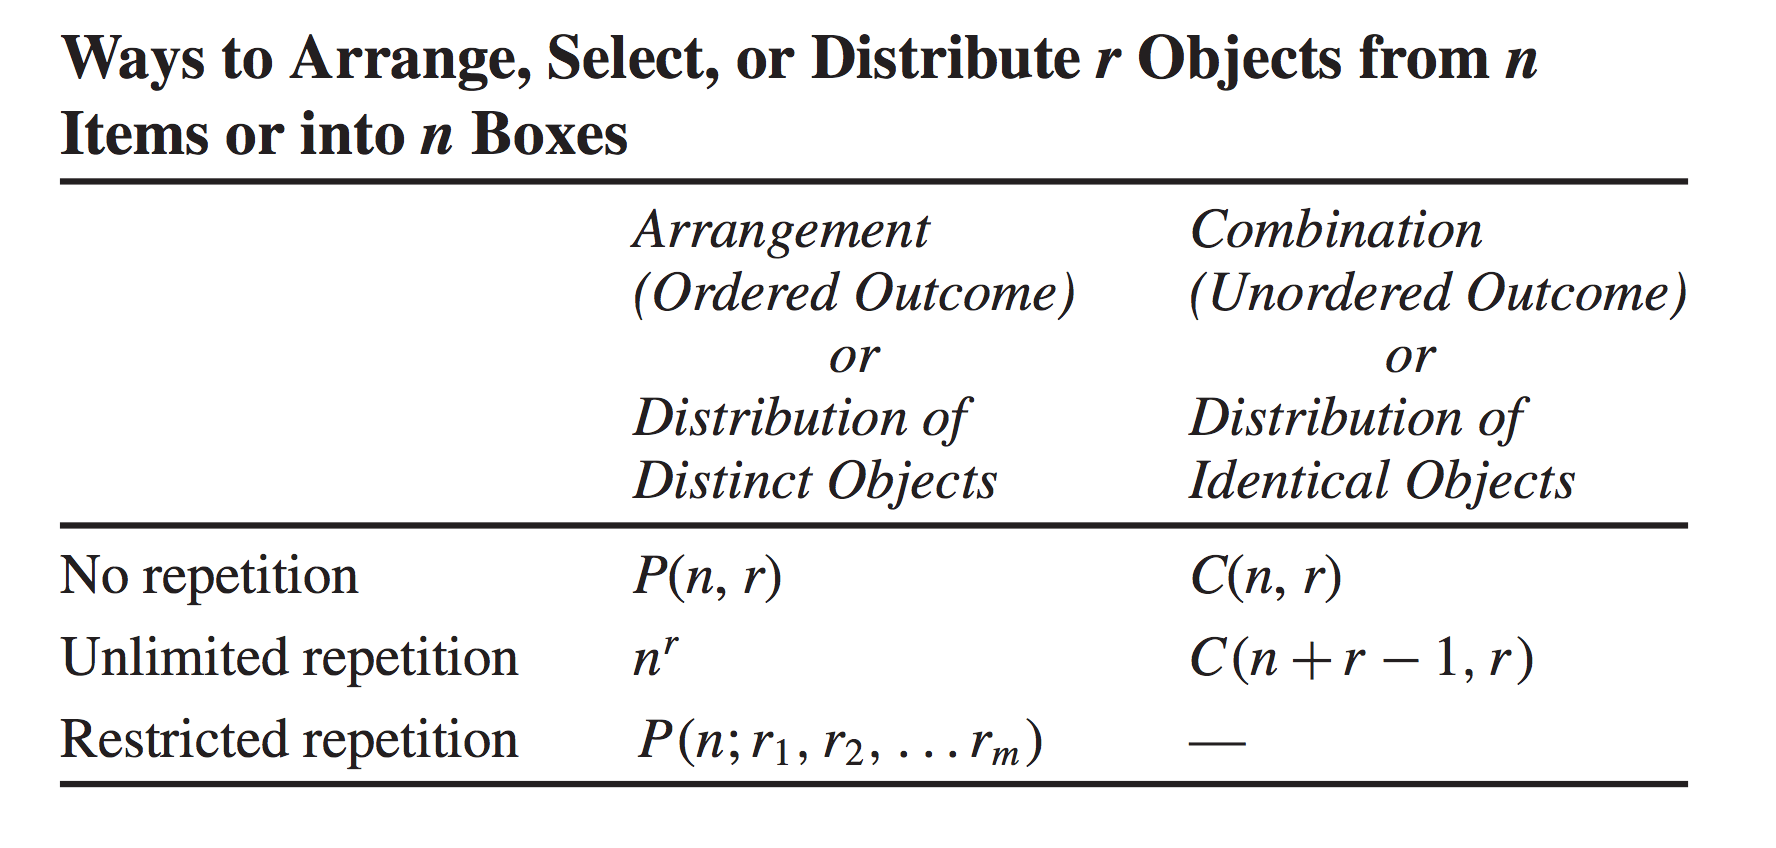
\includegraphics[width=300pt]{img/discrete-mathematics-tucker-combinatorics-summary.png}
\end{mdframed}

\begin{theorem*}[Subtuples]~\\
  The number of $k$-tuples that can be formed from a set of size $n$ without replacement is
  \begin{align*}
    (n)_k := n \cdot (n-1) \cdots (n - k + 1) = \frac{n!}{(n-k)!}.
  \end{align*}
\end{theorem*}

\begin{remark*}
  As a special case, the number of $n$-tuples (i.e. permutations/arrangements) is $n!$. (This is also
  the number of $n-1$ tuples.)
\end{remark*}

\begin{theorem*}[Subsets]~\\
  The number of subsets of size $k$ that can be formed from a set of size $n$ is
  \begin{align*}
    C(n, k) = {n \choose k} := \frac{(n)_k}{k!} = \frac{n!}{(n-k)!~k!}.
  \end{align*}
\end{theorem*}

\begin{proof}
  Each distinct $k$-subset gives rise to $k!$ $k$-tuples by assigning position labels. Therefore
  $(n)_k = {n \choose k}k!$.
\end{proof}

\begin{theorem*}[Multiset arrangements]~\\
  Consider a multiset comprising $n$ distinct elements, with $r_i \geq 1$ repeats of the $i$-th
  element. The number of $n$-tuples that can be formed from such a multiset is
  \begin{align*}
    P(n; r_1, \ldots, r_k)
    :=& {n \choose r_1}{n - r_1 \choose r_2}\cdots{n - r_1 \cdots - r_{n-1} \choose r_n}\\
    % &=\frac{n!}{(n - r_1)!r_1!}
    %   \frac{(n - r_1)!}{(n - r_1 - r_2)!r_2!}
    %   \cdots
    %   \frac{(n - r_1 \cdots - r_{n-1})!}{r_n!}
     =& \frac{n!}{r_1!r_2!\cdots r_n!}.
  \end{align*}
\end{theorem*}

\begin{proof}
  The $r_1$ copies of the first element must all go somewhere. ${n \choose r_1}$ counts the number
  of distinct positions they can occupy. Then there are $n - r_1$ empty positions left. Etc.
\end{proof}

\begin{remark*}
  The number $n!$ of permutations of a set is a special case of this with $r_i = 1$ for all $i$.
\end{remark*}

\begin{example*}~\\
  \begin{enumerate}
  \item {\bf How many ways are there to assign 100 different diplomats to five different
      continents?}\\
    $5^{100}$
  \item {\bf How many ways if 20 diplomats must be assigned to each continent?}\\
    $P(100; 20, 20, 20, 20, 20)$. Arrange the 100 diplomats in an arbitrary order. Now we have a
    multiset of country labels with 20 repeats of each label. Given the fixed ordering of the
    diplomats, there's a one-to-one correspondence between distinct permutations of the multiset
    and assignments of diplomats to countries.
  \item {\bf How many ways are there to distribute 20 (identical) sticks of red licorice and 15
    (identical) sticks of black licorice among five children?}\\
  ${20 + 5 -1 \choose 5 - 1}$${15 + 5 -1 \choose 5 - 1}$.
  \end{enumerate}
\end{example*}

\begin{theorem*}
  How many $k$-tuples for $k \leq n$ can be formed from such a multiset?
\end{theorem*}
\red{TODO}

\begin{theorem*}[Stars and bars]~\\
  Consider the number of ways that $n$ identical objects can be put into $k$ buckets, recording
  only the counts in each bucket (not the identities of the objects).

  With no empty buckets, the answer is
  \begin{align*}
    {n - 1 \choose k - 1} ~~~~~~~\text{($k-1$ bars to be placed in $n-1$ gaps between $n$ stars)}.
  \end{align*}

  With empty buckets allowed, the answer is
  \begin{align*}
    {n + k - 1 \choose k - 1} = P(n + k - 1; n, k - 1)~~~~~~~\text{(number of arrangements of $n$ stars and $k-1$ bars)}.
  \end{align*}
\end{theorem*}

\begin{proof}
  Represent this as $n$ unlabeled stars, and $k-1$ bars representing the partition of the stars
  into different buckets.

  With no empty buckets allowed, there are $n-1$ gaps where the bars can be placed, hence
  ${n - 1 \choose k - 1}$ ways of dividing up the items.

  With empty buckets allowed, there could be multiple bars in the same position. The number of
  $(n + k - 1)$-tuples that can be formed from the star and bar symbols is
  \begin{align*}
    P(n + k - 1; n, k - 1) &= C(n + k - 1, k - 1)C(n, n)\\
                           &= C(n + k - 1, k - 1)\\
                           &= C(n + k - 1, n)C(k - 1, k - 1)\\
                           &= C(n + k - 1, n).
  \end{align*}

  Note that ${n - 1 \choose k - 1}$ for the no-empty-buckets version can also be derived as
  follows:
  \begin{enumerate}
  \item Place one item into each bucket.
  \item Now there are $n - k$ items into $k$ buckets and empty buckets are allowed for the
    subsequent allocations. So the answer is
    ${(n - k) + k - 1 \choose k - 1} = {n - 1 \choose k - 1}$ by the empty-buckets-allowed theorem.
  \end{enumerate}
\end{proof}

\begin{theorem*}[Stars and bars]~\\
  The number of ways that $n$ items can be put into $k$ buckets, with empty buckets allowed,
  recording only the counts in each bucket (not the identities of the items), is

\end{theorem*}

\begin{theorem*}[Partitions]~\\
  The number of ways that $n$ items can be put into $k$ buckets, with no empty
  buckets, recording the identities of the items in each bucket, is the number of
  \textit{partitions} of size $k$ of a set of size $n$. It is equal to the
  Stirling number of the second kind:
  \begin{align*}
    S(n, k) = \frac{1}{k!} \sum_{i=0}^k(-1)^i{k \choose i}(k-i)^n. ~~ \blue{\text{(check this)}}
  \end{align*}
\end{theorem*}

\begin{proof}
  \red{TODO}
\end{proof}

\begin{claim}
  Consider the assignment of $n$ items $x_1, x_2, \ldots, x_n$ to $k$ buckets. Define $S_i$ to be the sum of items assigned to bucket $i$. The assignments for which $\max_i S_i$ is minimized is the assignment for which $\Var S_i$ is minimized.
\end{claim}

Not true?

\begin{theorem*}[Identities]~\\
  \begin{align*}
    {m + n \choose r} = \sum_{i=0}^r {m \choose i}{n \choose r - i}
  \end{align*}
\end{theorem*}

\subsection{Tucker - Applied Combinatorics - Exercises}

\begin{enumerate}
\item[(5.1)] {\bf General Counting Method for Arrangements and Selections}
  \begin{enumerate}
  \item[(37)] {\bf If three distinct dice are rolled, what is the probability that the highest
      value is
      twice the smallest value?}\\~\\
    $\frac{(3 \times 2 \times 3) + (3 \times 3!)}{6^3}$\\~\\
    An outcome is a 3-tuple such as $(1,1,1)$. Outcomes that match the criterion belong to two
    disjoint subsets:
    \begin{enumerate}
    \item Outcomes with two distinct values, such as $(1,1,2)$. There are $3 \times 2 \times 3$
      such outcomes ($3$ choices of unordered pairs of numbers, each with two alternative labelings
      and $3$ distinct permutations).
    \item Outcomes with three distinct values, such as $(2,3,4)$. There are $3 \times 3!$ such
      outcomes ($1 + 2$ unordered triples of numbers, each with $3!$ distinct permutations)
    \end{enumerate}
  \end{enumerate}
  \newpage
\item[(5.2)] {\bf Simple arrangements and selections}
  \begin{enumerate}
  \item[(Example 2)] {\bf How many ways are there to arrange the 7 letters of the word SYSTEMS...}
    \begin{enumerate}
    \item {\bf ...?}\\
      \begin{align*}
        7_{(7 - 3)} = 7\cdot 6\cdot 5\cdot 4 ~~~~~~~\text{(Choose positions of the other 4 letters, then Ss determined.)}
      \end{align*}
    \item {\bf ...with the 3 Ss consecutive?}
      \begin{align*}
        5_{(5)} = 5! ~~~~~~~\text{(Consider as 5-letter word S$^3$YTEM.)}
      \end{align*}
    \item {\bf ...with E before M?}
      \begin{align*}
        {7 \choose 2}5_{(5 - 3)} = {7 \choose 2}5\cdot 4 ~~~~~~~\text{(Choose position of E,M, then choose position of non-Ss.)}
      \end{align*}
    \item {\bf ...with E before M and 3 Ss consecutive?}
      \begin{align*}
        {5 \choose 2} 3! ~~~~~~~\text{(Consider as 5-letter word S$^3$YTEM, choose position of E,M, then choose positions for remaining letters.)}
      \end{align*}
    \end{enumerate}
  \item[(Example 6)] How
  \end{enumerate}
\end{enumerate}


\subsection{Generating functions}

\begin{definition*}[Generating function]
  Let $a_r$ be the number of ways to select $r$ objects in some counting procedure. Then $g(x)$ is
  a generating function for $a_r$ if $g(x)$ has the polynomial expansion
  \begin{align*}
    a_0 + a_1x + \ldots + a_nx^n.
  \end{align*}
\end{definition*}


\begin{example*}
  Find the generating function for $a_r$, the number of ways to select $r$ balls from $3$ green,
  $3$ white, $3$ blue, and $3$ gold balls.


\end{example*}

\newpage
\section{Pythagorean triples}

\subsection*{Project Euler question 9}

\begin{mdframed}
  A Pythagorean triplet is a set of three natural numbers, $a < b < c$, for which
  $a^2 + b^2 = c^2$.  For example, $3^2 + 4^2 = 9 + 16 = 25 = 5^2$.

  There exists exactly one Pythagorean triplet for which $a + b + c = 1000$.  Find the product
  $abc$.
\end{mdframed}

\begin{proof}~\\
  Let $m, n \in \N$.

  Recall that $|m + ni| := \sqrt{m^2 + n^2}$ and that $|wz| = |w| |z|$ for $w, z \in \C$.

  Note that $|(m + ni)^2| = |(m^2 - n^2) + 2mni| = m^2 + n^2 \in \Z$.

  Therefore $(m^2 - n^2, 2mn, m^2 + n^2)$ is a pythagorean triple for all $m, n \in
  \N$. (Claim: all pythagorean triples are of this form.)

  Therefore we seek $m, n \in \Z$ such that $m > n$ and
  \begin{align*}
    m^2 - n^2 + 2mn + m^2 + n^2             &= 1000\\
    m^2 + mn                                &= 500\\
    \(m + \frac{n}{2}\)^2 - \frac{n}{4} - 500 &= 0\\
    m                                       &= \sqrt{\frac{n}{4} + 500} - \frac{n}{2}
  \end{align*}
  Therefore (?) $\sqrt{\frac{n}{4} + 500} \in \Z$. So $\frac{n}{4} + 500 = a^2$
  for some $a \in \Z$.


\end{proof}


\chapter{Linear Algebra}
\section{Vector spaces and fields}\label{real-and-complex-vector-spaces}
A vector in a vector space is just something which can be added to another vector from the vector
space, and scaled by a scalar from the associated field. A vector does not involve any numbers until
it is represented as a linear combination of basis vectors, using nunbers from the associated
field. So whether something is a ``real vector space'' or a ``complex vector space'' depends only on
the field. If the field is $\R$ it is a real vector space; if the field is $\C$ it's a complex
vector space. It doesn't make sense to ask whether the vectors themselves are real or complex.

A \defn{field} is a set which is an abelian group under both addition and multiplication.

A \defn{vector space} is an additive abelian group $X$, together with a field $F$, such that $X$ is
closed under linear combinations with scalars from the field $F$.

\subsubsection{Examples}

% TODO:
% \begin{itemize}
% \item clarify: is $\C$ a field or a vector space or both?
% \item What is a one-dimensional complex vector space?
% \end{itemize}

\begin{enumerate}
\item $\R$ is a field.

\item $\R^2$ is not a field; multiplication is undefined.

\item If we equip $\R^2$ with complex multiplication then this is the field called $\C$.

\item The additive abelian group $\R$, together with the field $\R$, is a one-dimensional vector space.

  {\bf Proof:} Let $x \in \R$ with $x \neq 0$. Then $\{x\}$ is a basis for $\R$, since every element of $\R$ can
  be expressed uniquely as a scalar multiple of $x$. So $\R$ is one-dimensional.

\item The additive abelian group $\R^n$, together with the field $\R$, is a vector space. It is $n$-dimensional.

\item The additive abelian group $\C$, together with the field $\R$, is a two-dimensional vector
  space. It is isomorphic to $\R^2$.

\item The additive abelian group $\C$, together with the field $\C$, is a one-dimensional vector space.

  {\bf Proof:} Let $z \in \C$ with $z \neq 0$. Then $\{z\}$ is a basis for $\C$, therefore $\C$ as a
  complex vector space is one-dimensional.
\end{enumerate}

\newpage
\section{Examples of vector spaces}
\begin{enumerate}
\item The set $\R^n$ of $n-$tuples of real numbers, under componentwise addition and componentwise
  multiplication by real scalars.
\item Complex numbers
  \begin{enumerate}
  \item $\C$ under addition with multiplication by scalars from $\C$ is a field, and therefore a
    vector space. It is one-dimensional ($1$ and $i$ are not linearly independent).
  \item The set $\C^n$ of $n-$tuples of complex numbers, under componentwise addition and
    componentwise multiplication by complex numbers.
  \item $\C$ under addition with multiplication by real scalars is equivalent to $\R^2$.
  \end{enumerate}
\item Matrices \& linear transformations:
  \begin{enumerate}
  \item The set $M_{m \times n}(\R)$ of $m\times n$ matrices is a vector space, under componentwise
    addition and multiplication by real scalars.
  \item The set $\mathrm{Hom}(V, W)$ of linear transformations from vector space $V$ to vector
    space $W$ is a vector space: for scalar $a$, define $(aT)(v) := a(T(v))$, and
    $(S + T)v := S(v) + T(v)$.
  \end{enumerate}
\item The set $\R_n[x]$ of polynomials of degree $\leq n$ is a real vector
  space.
\item The set $\R^X$ of real-valued functions on any set $X$ is a real vector
  space. Examples:
  \begin{enumerate}
  \item Let $[n] = \{1, 2, \ldots, n\}$. Note that the function space $\R^{[n]}$ is
    the same as $\R^n$ (both are sets of $n-$tuples of reals).
  \item Similarly, $\R^{[m]\times[n]}$ is the same as $M_{m \times n}(\R)$.
  \item $\R^\R$, the set of all functions $\R\to\R$.
  \item The set of continuous functions $\R \to \R$, and differentiable functions
    $\R \to \R$, under pointwise addition and pointwise scalar multiplication
    (from any field?).
  \item Set of solutions of a homogeneous linear ODE
  \end{enumerate}
\item Sequences $(a_n)$ of real numbers, under term-wise addition and term-wise
  scalar multiplication, form a vector space, identifiable with the function
  space $\R^\N$. Examples:
  \begin{enumerate}
  \item Set of convergent sequences
  \end{enumerate}
\item The set of solutions of a system of \textit{homogeneous} linear equations
  in $n$ variables is a subspace $V$ of $\R^n$. (Let $A$ be the matrix
  representing the system and let $u$ and $v$ be solutions. Then $Au = Av = 0$
  and $V$ is a subspace since $A(u + v) = Au + Av = 0$, and
  $A(\lambda u) = \lambda Au = 0$.)
\end{enumerate}

\section{Linear systems}

Consider the linear systems
\begin{align*}
  \begin{array}{cc}
    \begin{cases}
      x = 0\\
      y = 0
    \end{cases}
    ~~~~~~~~~~~~~~~~~~~~~~~~~~~~&
    \begin{cases}
      x - y = 0\\
      x + y = 1\\
      x - z = 0
    \end{cases}
  \end{array}
\end{align*}

A ``solution'' is an assignment of values to the $n$ variables which makes all
$m$ equations true.

In other words, we notice that the equations involve $n$ variables, and
consider the set of $n$-tuples
$S = \{(x, y, \ldots) ~|~ x, y, \ldots \in \R\}$.

The set of solutions is the subset of $S$ for which all the equations are true.

Geometrically, we think of the 2-tuple $(a, b)$ as a point in the $\R^2$
plane. Specifically, if our basis is $\vec e_1, \vec e_2$, then $(a, b)$ is the
point $a\vec e_1 + b\vec e_2$. We might imagine that the basis is the standard
orthogonal basis, but that's not necessary.

The linear equations define hyperplanes (lines, planes etc) in $S$.

The set of solutions is the intersection of these hyperplanes: another
hyperplane or the empty set.

So at this point, we do not treat the ambient space as a vector space (we're
not adding or scaling points), and neither the equation hyperplanes nor the
solution hyperplane, need be a subspace (since it need not contain the origin).

Next, we rewrite the linear system as a matrix applied to a vector, $Ax = b$:
\begin{align*}
  \begin{array}{cc}
    \mat{1}{0}
        {0}{1} \vecMM{x}{y} = \vecMM{0}{0}
    ~~~~~~~~~~~~~~~~~~~~~~~~~~~~~~~~~~~~~~~&
    \matMMMxNN{1}{-1}
              {1}{~~1}
              {1}{-1} \vecMM{x}{y} = \vecMMM{0}{1}{0}.
  \end{array}
\end{align*}

The equation coefficients are now represented by a linear transformation
$A:\R^n \to \R^m$.

This matrix equation is saying:
\begin{enumerate}
\item Let the $x$ coefficients be a vector $\vec a_1 \in \R^m$. And let the $y$
  coefficients be another vector $\vec a_2 \in \R^m$, and so on.
\item So now you have $n$ vectors spanning some subspace of $\R^m$.
\item Is $b$ in their span? If so, for what values of $x, y, \ldots$ does
  $x\vec a_1 + y\vec a_2 + \cdots = b$?
\end{enumerate}

From Frenkel's Multivariable Calculus lectures:

\begin{center}
  \begin{quote}
    \textit{The dimensionality of an object is equal to the dimensionality of the
      ambient space, minus the number of independent equations.}
  \end{quote}
\end{center}

So, basically, suppose there are $n$ variables. Then the solution set is a
subset (hyperplane) of $\R^n$, and

\begin{tabular}{c|c}
  Independent equations & Solution set\\
  \hline
  1                     & $(n - 1)$-dimensional hyperplane \\
  2                     & $(n - 2)$-dimensional hyperplane \\
  \vdots                & \vdots \\
  $n-1$                 & line \\
  $n$                   & point \\
  $n + 1$               & impossible \\
  \vdots                & \vdots
\end{tabular}

So when do we get no solutions? That's when
\begin{align*}
  &\text{the $n$ columns of $A$ do not span $\R^m$}\\
  \iff &\Rank A < \text{(number of equations)}\\
  \iff &\text{not all equations independent},
\end{align*}
and $b$ is not in their span.

In other words, suppose we have a linear system involving $n$ variables.

Suppose that all the $m$ equations are independent: full row rank.

Then $m \leq n$.

Now we introduce a dependent equation into the system.

\red{One error above is that its only the coefficients of the equation that
  we're considering when we say the rows are dependent/independent. So it's not
  correct to talk about ``independent equations''.}


\section{Subspaces}
A subspace $U$ of $V$ is a subset of $V$ for which
\begin{enumerate}
\item $0 \in U$
\item For any finite subset $U^* \subset U$, the set of all linear combinations
  of $U^*$ is also a subset of $U$.
\end{enumerate}

\section{Span, basis, dimension}
\begin{theorem}
  Every basis has the same size.
\end{theorem}

\begin{proof} Let $v_1, \ldots, v_n$ be a basis for a vector space $V$.


\end{proof}

\begin{theorem}
  A spanning set that is the same size as a basis is also a basis.
\end{theorem}

\begin{proof}
  Let $v_1, \ldots, v_n$ be a basis for a vector space $V$, and let
  $u_1, \ldots, u_n$ span $V$.

  We know that $v_1, \ldots, v_n$ are linearly independent and that if we
  remove any one of them they will cease to span.

  We want to show that $u_1, \ldots, u_n$ are linearly independent.

  Suppose, that the $u_i$ are not linearly independent and that
  $u_2, \ldots, u_n$ span $V$. Thus there are $n-1$ vectors in this spanning
  set. But the Steinitz Exchange Lemma states that if $v_1, \ldots, v_n$ are
  linearly independent and $u_1, \ldots, u_m$ span, then $n \leq m$. This
  contradiction proves that the $u_i$ are linearly independent.
\end{proof}

\begin{theorem}\label{transformed-basis-is-a-basis}
  Let $U, V$ be vector spaces, let $f:U \to V$ be an invertible linear map, and let
  $e_1, \ldots, e_n$ be a basis for $U$. Then $f(e_1), \ldots, f(e_n)$ is a basis for $V$.
\end{theorem}

\begin{proof}We need to show that the $f(e_i)$ are linearly independent and spanning.

  \begin{enumerate}
  \item {\bf Linear independence}\\
    Suppose $\sumin \lambda_if(e_i) = 0$.

    Therefore $f\(\sumin \lambda_ie_i\) = 0$ since $f$ is linear.

    Therefore $\sumin \lambda_ie_i = f^\1(0) = 0$, since the preimage of $0$ is $\{0\}$ for an
    invertible linear map.

    But the $e_i$ are linearly independent, therefore $\lambda_i = 0$ for all $i = 1, \ldots n$, as
    required.

  \item {\bf Spanning}\\
    Let $v \in V$.

    Then $v = f(u)$ for some $u \in U$, since $f$ is surjective.

    Therefore $v = f\(\sumin \lambda_ie_i\) = \sumin \lambda_if(e_i)$ for some
    $\lambda_1, \ldots, \lambda_n$, as required.

  \end{enumerate}
\end{proof}

\begin{problem*}
  If $u, v$ are linearly independent under one basis are they linearly independent under all choices of basis?
\end{problem*}

\section{Linear transformations and matrices}

A linear transformation is completely specified by

\begin{enumerate}
\item Some basis vectors $i$ and $j$
\item Where those basis vectors are taken to by the transformation.
\end{enumerate}

How the transformation affects any other point follows from those two pieces of
information.

So $i$ might be taken to $ai + bj$, and $j$ might be taken to $ci + dj$.
In this case we would use the following matrix to describe the
transformation:

$$
\mat{a}{c}
    {b}{d}
$$

Some examples are

$$
\begin{array}{ll}
\text{stretch by a in the i-direction} & \mat{a}{0}
                                             {0}{1}
\\\\
\text{stretch by a in the i-direction and shear right} & \mat{a}{b}
                                                             {0}{1}
\\\\
\text{rotate anticlockwise 90°} & \mat{0}{-1}
                                      {1}{ 0}
\end{array}
$$

Note that we haven't said what $i$ and $j$ are yet; they \textit{define} the
2-dimensional space that we're considering. But, we can think of them for now
as the usual orthogonal unit vectors in 2D space.

So the matrix tells us where the basis vectors have been taken to. Any other
vector $fi + gj$ is taken to wherever that is using the transformed basis
vectors:

$$
fi + gj \longrightarrow f\cvec{a}{b} + g\cvec{c}{d} = \cvec{fa + gc}{fb + gd}
$$


And that's how matrix multiplication is defined:

$$
\mat{a}{c}
    {b}{d} \cvec{f}{g} = \cvec{fa + gc}{fb + gd}
$$


A matrix represents a linear transformation by showing where the basis vector
are taken to.

\begin{theorem}
  The inverse of a 2x2 matrix is...
\end{theorem}

\section{Geometric interpretation of matrix operations}
\url{https://math.stackexchange.com/questions/37398/what-is-the-geometric-interpretation-of-the-transpose}
\url{https://math.stackexchange.com/questions/598258/determinant-of-transpose/636198#636198}


\section{Commutativity}
\subsection{Examples of transformations that don't commute}
Let $A$ be reflection around the first coordinate axis $\matMMxNN{1}{0}
                                                                 {0}{-1}$
and let $B$ be $90\deg$ anticlockwise rotation $\matMMxNN{0}{-1}
                                                         {1}{0}$.

Then $BA = \matMMxNN{0}{1}
                    {1}{0}
\neq  AB = \matMMxNN{0}{-1}
                    {-1}{0}$.

Note that $A^\1 = A = A^T$ and $B^\1 = \matMMxNN{0}{1}
                                               {-1}{0} = B^T$.

Therefore these are both orthogonal (unitary) matrices.


\section{Eigenvalues, eigenvectors, characteristic polynomial}

Let $V$ be a vector space and let $T:V \to V$ be a linear transformation.

\begin{definition*}[eigenvalue]
  $\lambda$ is an \textit{eigenvalue} of $T$ iff there exists \todo{non-zero?} $v \in V$ such that
  $Tv = \lambda v$.
\end{definition*}

\begin{definition*}[eigenspace]
  $E_\lambda = \{v ~|~ Tv = \lambda v\}$ is an \textit{eigenspace} of $T$.
\end{definition*}

\begin{definition*}[eigenvector]
  An \textit{eigenvector} is a non-zero element of an eigenspace.
\end{definition*}

\begin{definition*}[characteristic polynomial]
  The characteristic polynomial of $T$ is $\chi_T(x) = \det(T - xI)$. Note that
  $\lambda$ is an eigenvalue of $T$ iff $x=\lambda$ is a root of $\chi_T(x)$.
\end{definition*}

\begin{intuition*}~\\
  Decompose $T$ as the sum of two transformations: $T = \lambda I + T^*$. This
  means that the effect of applying $T$ to a vector is the same as applying
  $\lambda I$ to the vector, and separately applying $T^*$ to the same vector,
  and adding the two results.

  Note that applying $\lambda I$ to a vector just scales the vector by $\lambda$.

  Note that $T^* = T - \lambda I$.

  Therefore what $T - \lambda I$ does to a vector is: whatever remains to be done after
  scaling by $\lambda$, in order to have the same effect as $T$.

  Suppose $\lambda$ is an eigenvalue. Then there exists an eigenspace
  $E_\lambda$ (a line, at least) containing vectors which are simply stretched
  by a factor $\lambda$. So for $v \in E_\lambda$, nothing remains to be done
  after scaling by $\lambda$, and so we have $(T - \lambda I)(v) = 0$.

  Therefore
  \begin{itemize}
  \item If $T - \lambda I$ has a nullspace containing a non-zero element, then
    $\lambda$ is an eigenvalue and the nullspace is the eigenspace for
    $\lambda$.
  \item The roots of $\det(T - xI)$ are the eigenvalues of $T$.
  \end{itemize}

\end{intuition*}

\begin{remark*}[Repeated eigenvalues]~\\
  If two eigenvectors share the same eigenvalue then they are in the same eigenspace.
\end{remark*}

\begin{proof}
  Suppose that $Tv_1 = \lambda v_1$ and $Tv_2 = \lambda v_2$ and
  $v_1 \neq v_2$, and let $a$ be a scalar.

  Then
  $T(v_1 + av_2) = T(v_1) + aT(v_2) = \lambda v_1 + a\lambda v_2 = \lambda(v_1
  + av_2)$.
\end{proof}



\begin{example*}
  $A = \mat
  {0}{-1}
  {1}{0}$ is a rotation anticlockwise by $90\deg$. So it should be found to not
  have any eigenvectors.

  So let's try to find the eigenvectors. The eigenvalues of $A$ are the solutions to
  $\det (A - \lambda I) = 1 -\lambda^2 = 0$, so $\lambda = 1, -1$.

  If $\lambda = 1$ then we have
  \begin{align*}
    \mat{0}{-1}{1}{0}\pvecc{x_1}{x_2} &= \pvecc{x_1}{x_2} \\
    \pvecc{-x_2}{x_1} &= \pvecc{x_1}{x_2},
  \end{align*}
  and if $\lambda = -1$ then we have
  \begin{align*}
    \mat{0}{-1}{1}{0}\pvecc{x_1}{x_2} &= \pvecc{-x_1}{-x_2} \\
    \pvecc{-x_2}{x_1} &= \pvecc{-x_1}{-x_2},
  \end{align*}
  so that $\pvecc{x_1}{x_2} = \pvecc{0}{0}$ is the only solution in both cases.
\end{example*}

\begin{example*}
  $A = \mat {\cos \theta}{-\sin \theta} {\sin \theta}{\cos \theta}$ is a rotation anticlockwise by
  $\theta \deg$. So it should be found to not have any eigenvectors.

  So let's try to find the eigenvectors. The eigenvalues of $A$ are the solutions to
  \begin{align*}
    \det (A - \lambda I)
    &= (\cos\theta - \lambda)^2 + \sin^2\theta \\
    &= \lambda^2 - 2\lambda\cos\theta + 1 \\
    &= 0,
  \end{align*}
  so that
  \begin{align*}
    \lambda
    &= \frac{2\cos\theta \pm \sqrt{4\cos^2\theta - 4}}{2} \\
    &= \cos\theta \pm \sqrt{\cos^2\theta - 1} \\
    &= \cos\theta \pm \sin\theta.
  \end{align*}

  If $\lambda = \cos\theta + \sin\theta$ then we have
  \begin{align*}
    \mat
    {\cos \theta}{-\sin \theta}
    {\sin \theta}{\cos \theta} \pvecc{x_1}{x_2}
    &= \pvecc{(\cos\theta + \sin\theta)x_1}{(\cos\theta + \sin\theta)x_2} \\
    \pvecc{x_1\cos\theta - x_2\sin\theta}{x_1\sin\theta + x_2\cos\theta}
    &= \pvecc{(\cos\theta + \sin\theta)x_1}{(\cos\theta + \sin\theta)x_2} \\
    \begin{cases}
      x_1\sin\theta = -x_2\sin\theta \\
      x_1\sin\theta = x_2\sin\theta.
    \end{cases} \\
    \begin{cases}
      \sin\theta(x_1 + x_2) = 0 \\
      \sin\theta(x_1 - x_2) = 0,
    \end{cases}
  \end{align*}
  so either $\theta = 2\pi k$ or $\pvecc{x_1}{x_2} = 0$, as expected.

\end{example*}



\section{Change of basis}

Suppose person B uses some other basis vectors to describe locations in
space. Specifically, in our coordinates, their basis vectors are
$\scvec{2}{1}$ and $\scvec{-1}{1}$.


\textbf{When they state a vector, what is it in our coordinates?}

If they say $\scvec{-1}{2}$, what is that in our coordinates?

Well, if they say $\scvec{1}{0}$, that's $\scvec{2}{1}$ in our coordinates. And
if they say $\scvec{0}{1}$, that's $\scvec{-1}{1}$ in our coordinates. So the
matrix containing \textit{their basis vectors expressed using our coordinate system}
transforms a point expressed in their coordinate system into one expressed in
ours. That last sentence is critical, so hopefully it makes sense! So, the answer is

$$
\mat{2}{-1}
    {1}{ 1} \cvec{-1}{2} = \cvec{-4}{1}.
$$


\textbf{When we state a vector, what is it in their coordinates?}

We give the vector $\scvec{3}{2}$. What is that in their coordinate system? By
definition, the answer is the weights that scales their basis vectors to hit
$\scvec{3}{2}$. So, the solution to

$$
\mat{2}{-1}
    {1}{1} \cvec{a}{b} = \cvec{3}{2}.
$$


Computationally, we can see that we can get the solution by multiplying both
sides by the inverse:

$$
\cvec{a}{b} = \mat{2}{-1}
                  {1}{1}^{-1} \cvec{3}{2}.
$$

Conceptually, we have

$$
\mat{2}{-1}
    {1}{1} =
\begin{pmatrix}\text{matrix converting their}\\\text{representation to ours} \\ \end{pmatrix}
$$

where ``their representation'' means the vector expressed using their coordinate
system. So the role played by the inverse is

$$
\cvec{a}{b} =
\begin{pmatrix}\text{matrix converting our}\\\text{representation to theirs} \\ \end{pmatrix}
\cvec{3}{2}.
$$

\textbf{When we state a transformation, what is it in their coordinates?}

We state a 90° anticlockwise rotation of 2D space:

$$
\mat{0}{-1}
    {1}{0}
$$

what is that transformation in their coordinates? The answer is

$$
\begin{pmatrix}\text{matrix converting our}\\\text{representation to theirs} \\ \end{pmatrix}
\mat{0}{-1}
    {1}{0}
\begin{pmatrix}\text{matrix converting their}\\\text{representation to ours} \\ \end{pmatrix}
$$

since the composition of those three transformations defines a single
transformation that takes in a vector expressed in their coordinate system,
converts it to our coordinate system, transforms it as requested, and then
converts back to theirs.

Let
\begin{align*}
  P = \mat{2}{-1}
          {1}{1}
\end{align*}
be the change-of-basis matrix . Then the matrix, in their coordinates, of the
rotation transformation is
$$
P^\1\mat{0}{-1}
        {1}{0} P.
$$

What about the uniform stretch transformation? In our coordinates this has
matrix $\lambda I = \mat{\lambda}{0}
                        {0}{\lambda}$. In their coordinates, it has matrix
\begin{align*}
P^\1\lambda I P = \lambda P^\1 P = \lambda I.
\end{align*}
I.e. a uniform stretch transformation represented by a diagonal matrix has the
same matrix in any basis. That's because -- forget about introducing any basis
-- there is only one ``uniform stretch transformation'': it's the
transformation that acts on space like it's a balloon being inflated
uniformly. Whatever basis vectors you choose, each one $\vec e_i$ is going to be taken
to $\lambda \vec e_i$. That means the matrix of the transformation, in whatever basis,
is $\mat{\lambda}{0}
        {0}{\lambda}$, because the vector
\begin{quote}
``one unit in the $\vec e_1$ direction, zero units in the $\vec e_2$ direction''
\end{quote}
is going to be taken to the vector
\begin{quote}
``$\lambda$ units in the $\vec e_1$ direction, zero units in the $\vec e_2$ direction''.
\end{quote}

What about a non-uniform stretch transformation?

\newpage
Consider $\R^2$. Fix a first basis vector $e_1$.

Consider the map $T:\R^2\to\R^2$ which stretches space by a factor of 2 in the
direction of $e_1$, and by a factor of 3 in the orthogonal direction.

Suppose that the second basis vector $e_2$ is orthogonal to $e_1$ and has the
same magnitude.

Then the matrix of $T$ is $\mat{2}{0}
                               {0}{3}$ with respect to this basis.
~\\

Now consider an alternative basis $\{f_1, f_2\}$ where $f_2$ intersects with
$f_1$ at $45\deg$.

Specifically, with respect to basis $\{e_1, e_2\}$, we have $f_1 = (1, 0)$ and
$f_2 = (1, 1)$.

Then the matrix of $T$ with respect to basis $\{f_1, f_2\}$ is
\begin{align*}
  \mat{1}{1}
      {0}{1}^\1 \mat{2}{0}
                    {0}{3} \mat{1}{1}
                               {0}{1} &=
  % \mat{1}{-1}
  %     {0}{1} \mat{2}{0}
  %                {0}{3} \mat{1}{1}
  %                           {0}{1} \\ &=
  \mat{1}{-1}
      {0}{1}  \mat{2}{2}
                  {0}{3} \\ &=
  \mat{2}{-1}
      {0}{3}.
\end{align*}
(It's obvious that $f_1 \mapsto (2, 0)$; that $f_2 \mapsto (-1, 3)$ is clear in
a diagram.)

The eigenvalues of $T$ are clearly 2 and 3, independent of basis.

The eigenspaces are the line through $e_1$, and the line through $e_2$.

So with respect to basis $\{e_1, e_2\}$, the eigenspaces are
$\{(a, 0) ~|~ a \in \R\}$ and $\{(0, a) ~|~ a \in \R\}$.

And with respect to basis $\{f_1, f_2\}$, the eigenspaces are
$\{(a, 0) ~|~ a \in \R\}$ and $\{(-a, a) ~|~ a \in \R\}$.

  % The characteristic polynomial is $\det(A - \lambda I) = 0$, where $A$ is a
  % matrix of $T$ with respect to some basis. Let $A = \mat{2}{0}
  % {0}{3}$. Then
  % \begin{align*}
  %   \det(A - \lambda I) = \det \mat{2 - \lambda}{0}
  %   {0}{3 - \lambda} = (2 - \lambda)(3 - \lambda).
  % \end{align*}
  % So the eigenvalues are 2 and 3.

  % The eigenspace $E_2$ with respect to basis $\{e_1, e_2\}$ is the set of
  % solutions to
  % \begin{align*}
  %   \mat{2}{0}
  %   {0}{3} \vecMM{x}{y} = \vecMM{2x}{2y}.
  % \end{align*}

\newpage
Consider the map which stretches space by a factor of 2 in one direction, and a
factor of 3 in another direction.

Then there exists a basis for which the map has matrix
$
\mat{2}{0}
    {0}{3}
$.

What are the eigenspaces of this map?

The characteristic polynomial (basis independent) is $\det(A - \lambda I) = 0$
where $A$ is the matrix of the map wrt some basis.

\newpage
\section{Symmetric matrices}

\textbf{Spectral theorem for symmetric matrices}

Symmetric $n \by n$ matrix $A$ (real).

$A^\1 = A^\T$

$n$ orthogonal eigenvectors with real eigenvalues.

Orthonormal matrix $U$ containing normalized eigenvectors.

$A = U\Lambda U^\1 = U\Lambda U^\T$

(Eigenvalues are uniquely determined by matrix. Eigenvalues can be repeated, in which case any linear combination of their
eigenvalues is also an eigenvalue.)

\section{Inner Product Spaces}

Note that if $f(\cdot)$ is linear:
\begin{enumerate}
\item $f(ax + by) = f(ax) + f(by)$.
\end{enumerate}

\begin{definition*}[Bilinear form]~\\
  A bilinear form is a binary function $f(\cdot, \cdot)$ such that:
  \begin{enumerate}
  \item $f(ax + by, z) = f(ax, z) + f(by, z)$
  \item $f(z, ax + by) = f(z, ax) + f(z, by)$.
  \end{enumerate}
\end{definition*}


\begin{claim*}
  The dot product in $\F^n$ is bilinear.
\end{claim*}

\begin{proof}
  \begin{align*}
    \langle ax + by , z \rangle :=& \sum_i (ax + by)_iz_i\\
                                 =& \sum_i (ax_i + by_i)z_i\\
                                 =& \sum_i ax_iz_i + \sum_i by_iz_i\\
                                 =& \langle ax, z \rangle + \langle by, z \rangle\\
    \langle z, ax + by \rangle  :=& \ldots
  \end{align*}
\end{proof}

Note that $\langle x, y \rangle = x \cdot y = x^Ty = x^TIy$.

And note that the ``quadratic form'' $ax^2 + 2bxy + cy^2$ can be written as
\begin{align*}
\x^\T A \x = \cvec{x}{y}^\T \mat{a}{b}
                                {b}{c} \cvec{x}{y}.
\end{align*}
This is a scalar. In general, a quadratic form for symmetric matric $A$ is
\begin{align*}
\x^\T A \y = \sum_{jk}A_{jk}x_jy_k.
\end{align*}

These quadratic forms are also bilinear forms: the dot product is a quadratic form using the
identity matrix.

\begin{definition*}[Gram matrix]
  Take a collection of vectors $v_1, \ldots, v_n$. A Gram matrix is the $n \times n$ matrix
  $(\langle v_i, v_j \rangle)$.
\end{definition*}

\begin{theorem*}
  Every bilinear form is of the form $\langle u, v \rangle = u^TAv$ for some Gram matrix.
\end{theorem*}

\begin{definition*}
  A bilinear form is symmetric if $\langle u, v \rangle = \langle v, u \rangle$.
\end{definition*}

\begin{theorem*}
  The bilinear form $\langle u, v \rangle := u^TAv$ is symmetric if and only if $A$ is symmetric.
\end{theorem*}

\begin{definition*}
  A \red{TODO (real?)} bilinear form is positive definite if $\langle u, v \rangle > 0$ for all
  $v \in V \setminus \{0\}$. \red{TODO that doesn't make sense}
\end{definition*}

\begin{definition*}[Inner product]~\\
  An inner product is a bilinear form that is symmetric and positive definite.

  An inner product space is a vector space equipped with an inner product.

  In an abstract inner product space we define the angle between $u$ and $v$ to be
  $\cos^\1\Big(\frac{\langle u, v \rangle}{\norm{u}\norm{v}}\Big)$.

  In a real inner product space we define the norm to be $\norm{u} := \sqrt{\langle u, u \rangle}$.
\end{definition*}

\begin{theorem*}[Cauchy-Schwartz inequality]~\\
  Let $V$ be an inner product space and let $u, v \in V$. Then
  $\langle u, v \rangle \leq \norm{u} \norm{v}$.
\end{theorem*}

\begin{proof}
  \red{Are we assuming the inner product is real-valued here?}
  Define $f(t) := \langle tu + v, tu + v \rangle = \norm{tu +v}^2$.

  Use bilinearity and symmetry to show that
  $f(t) = t^2 \langle u, u \rangle + 2t \langle u, v \rangle + \langle v, v \rangle$. (How?)

  The Cauchy-Schwartz inequality follows by noting that the determinant of this quadratic must be
  negative.
\end{proof}

\section{Complex vector spaces}
When viewed as a real vector space (i.e. with real scalars), $\C$ is
two-dimensional, e.g. $\{1, i\}$ is a basis.

When viewed as a complex vector space (i.e. with complex scalars), $\C$ is one-dimensional: $\{1\}$
is a basis; $\{1, i\}$ are no longer linearly independent.

\footnotetext{
  \href{https://www.youtube.com/playlist?list=PLZHQObOWTQDPD3MizzM2xVFitgF8hE_ab}{Essence of Linear Algebra} video series by \href{http://www.3blue1brown.com/}{Grant Sanderson / 3blue1brown}
}

\begin{definition*}
  Let $V$ be a complex vector space.

  $\langle \cdot, \cdot \rangle:V \times V \to \C$ is a sesquilinear form if
  \begin{enumerate}
  \item $\langle au + bv, z \rangle = a\langle u, z \rangle + b\langle v, z \rangle$
  \item $\bar{\langle u, u \rangle} = \langle u, u \rangle$ (therefore
    $\langle u, u \rangle \in \R$).
  \end{enumerate}
\end{definition*}


\begin{definition*}[Hermitian space]~\\
  Let $V$ be a complex vector space (i.e. complex scalars).

  A Hermitian form is a sesquilinear form that is symmetric and positive definite.

  A complex inner product space, or Hermitian space, is a complex space equipped with a Hermitian
  form as an inner product.
\end{definition*}


\section{Finding the nth Fibonacci number via an eigenvector change of basis}


This is the problem given at the end of the eigenvectors video in the
Essence of Linear Algebra\footnote{\url{https://www.youtube.com/playlist?list=PLZHQObOWTQDPD3MizzM2xVFitgF8hE_ab}}
series by 3blue1brown\footnote{\url{http://www.3blue1brown.com/}}.


\subsection*{Introduction}

Consider the matrix

$$
A = \mat{0}{1}
        {1}{1}
$$

The first few powers are

\begin{align*}
&A^{1} &= \mat{0}{1}
              {1}{1}
\\
&A^{2} = \mat{0}{1}
             {1}{1} \mat{0}{1}
                        {1}{1} &= \mat{1}{1}
                                      {1}{2}
\\
&A^{3} = \mat{0}{1}
             {1}{1} \mat{1}{1}
                        {1}{2} &= \mat{1}{2}
                                      {2}{3}
\\
&A^{4} = \mat{0}{1}
             {1}{1} \mat{1}{2}
                        {2}{3} &= \mat{2}{3}
                                      {3}{5}
\end{align*}

The Fibonacci sequence is the sequence you get by starting with $0,
1$ and after that always forming the next number by adding the two previous ones:
$F_0, F_1, F_2, F_3, F_4, F_5, F_6, F_7, ...$ = $0, 1, 1, 2, 3, 5, 8, 13, ...$.

The matrix powers are generating the Fibonacci sequence:
\begin{align*}
  A^{n} = \mat{F_{n-1} }{F_n      }
  {F_n     }{F_{n+1} }
\end{align*}
So if there were a way to compute the $\nth$ power of that matrix ``directly'',
that would also be a way to compute the $\nth$ Fibonacci number ``directly'',
i.e. without computing all the preceding Fibonacci numbers \textit{en route}.

How can we do this? To state the problem in a different way, we need to
construct a new matrix that performs exactly the same transformation as $A^n$,
but which somehow does the exponentiation step ``in one go'' rather than by
multiplying $A$ with itself $n$ times.

\subsection*{Solution outline}

Matrices represent transformations, so we can talk about them as taking in some
vector and producing some other vector. The approach we're going to take is to
re-express the $A^n$ transformation as follows:

\begin{enumerate}
\item Convert the input vector to its representation in an alternative basis which uses the
  eigenvectors as the basis vectors (it's called an ``eigenbasis'').
\item In this alternative basis, compute the new position of the vector after carrying out the
  $A^n$ transformation.
\item Convert the resulting vector back to its representation in our original basis.
\end{enumerate}

I.e., we're going to compute the overall transformation as this product of
matrices (remember that one reads these things right-to-left):
\begin{align*}
  \begin{pmatrix}\text{matrix converting their}\\\text{representation to ours} \\ \end{pmatrix}
  \begin{pmatrix}\text{matrix that does the A transformation}\\\text{in the alternative basis} \\ \end{pmatrix}^n
  \begin{pmatrix}\text{matrix converting our}\\\text{representation to theirs} \\ \end{pmatrix}
\end{align*}
The crux of all this is that the exponentiation is efficient in the
eigenbasis. That's because, in the eigenbasis, the transformation is just
stretching space in the directions of the two basis vectors. So to do the
transformation $n$ times in the eigenbasis, you just stretch by the
stretch-factor raised to the $\nth$ power, rather than doing $n$ matrix
multiplications.

\subsection*{Solution details}

Let's suppose we've already found the eigenvectors, and that there are two of
them, and that we've arranged them as the two columns of a matrix $V$. $V$ holds
the basis vectors of the alternative basis, and therefore we know from the
[change of basis](\url{./linear-algebra.html#change-of-basis}) notes that $V$ is the
matrix that takes as input a vector expressed in the alternative basis and
outputs its representation in our basis.

So, step (3) is done by $V$, and step (1) is done by $V^{-1}$, and the matrix
performing all three steps is going to look like
\begin{align*}
  V
  \begin{pmatrix}\text{matrix that does the A transformation}\\\text{in the alternative basis} \\ \end{pmatrix}^n
  V^{-1}
\end{align*}
OK, so what is the matrix in the middle? The [change of
basis](\url{./linear-algebra.html#change-of-basis}) notes tell us that we can compute it as
\begin{align*}
  \begin{pmatrix}\text{matrix converting our}\\\text{representation to theirs} \\ \end{pmatrix}
  A
  \begin{pmatrix}\text{matrix converting their}\\\text{representation to ours} \\ \end{pmatrix}
\end{align*}
In other words the matrix in the middle is
\begin{align*}
  V^{-1}AV
\end{align*}
and the entire transformation is
\begin{align*}
  V
  \Big(V^{-1}AV\Big)^n
  V^{-1}
\end{align*}
Put back into words, that's
\begin{align*}
  \begin{pmatrix}\text{matrix converting their}\\\text{representation to ours} \\ \end{pmatrix}
  \Bigg(
  \begin{pmatrix}\text{matrix converting our}\\\text{representation to theirs} \\ \end{pmatrix}
  A
  \begin{pmatrix}\text{matrix converting their}\\\text{representation to ours} \\ \end{pmatrix}
  \Bigg)^n
  \begin{pmatrix}\text{matrix converting our}\\\text{representation to theirs} \\ \end{pmatrix}
\end{align*}

Recall that above we observed that the $\nth$ power of $A$ is a matrix with the
nth Fibonacci number in its bottom left and top right entries. So the following
tasks remain:
\begin{enumerate}
\item Find the eigenvectors and put them in a matrix $V$.
\item Find the inverse of $V$.
\item Compute the matrix product $V^{-1}AV$.
\item Compute the result of raising that to the $\nth$ power.
\item Plug the result of that into the overall expression.
\item Take the entry in the bottom left or top right (they should be the same!).
\end{enumerate}

The result should be an expression giving the $\nth$ Fibonacci number as a
function of $n$. It should be possible to give as input to that function the
number one million, and have it output the one millionth Fibonacci number
directly, without it having to go through the preceding 999,999 Fibonacci
numbers.


\subsection*{The answer without showing the calculations}

\begin{align*}
&\text{The eigenvectors are}
\\\\
&V &= \mat{2          }{2          }
        {1 + \sqrt 5}{1 - \sqrt 5}
\\\\
&\text{which has inverse}
\\\\
&V^{-1} &= \frac{-1}{4\sqrt 5} \mat{1 - \sqrt 5 }{-2}
                                 {-1 - \sqrt 5}{2}
\\\\
&\text{Therefore}
\\\\
&V^{-1}AV &= \frac{1}{2} \mat{1 + \sqrt 5}{0          }
                            {0          }{1 - \sqrt 5}
\\\\
&\text{and}
\\\\
&(V^{-1}AV)^n &= \frac{1}{2^n} \mat{(1 + \sqrt 5)^n}{0          }
                                   {0                }{(1 - \sqrt 5)^n}
\\\\
&\text{and}
\\\\
&V \Big(V^{-1}AV\Big)^n V^{-1} &=
\mat{\frac{\big((1 + \sqrt 5)^{n-1} - (1 - \sqrt 5)^{n-1}\big)}{2^{n-1}\sqrt 5}}{\frac{\big((1 + \sqrt 5)^n     - (1 - \sqrt 5)^n    \big)}{2^n    \sqrt 5}}
    {\frac{\big((1 + \sqrt 5)^n     - (1 - \sqrt 5)^n    \big)}{2^n    \sqrt 5}}{\frac{\big((1 + \sqrt 5)^{n+1} - (1 - \sqrt 5)^{n+1}\big)}{2^{n+1}\sqrt 5}}
\\\\
&\text{Therefore the nth Fibonacci number is}
\\\\
&F_n &= \frac{(1 + \sqrt 5)^n     - (1 - \sqrt 5)^n}
             {2^n    \sqrt 5}
\end{align*}

\newpage
\subsection*{Does this actually work?}

Yes.

\begin{minted}{python3}
    from math import sqrt

    def fib(n):
        return (
            ( (1 + sqrt(5))**n - (1 - sqrt(5))**n )
            /
            float(2**n * sqrt(5)))

    for i in range(10):
        print(i, fib(i))

    0 0.0
    1 1.0
    2 1.0
    3 2.0
    4 3.0
    5 5.0
    6 8.0
    7 13.0
    8 21.0
    9 34.0
\end{minted}

\subsection*{History}

The formula is known as
Binet's formula (\url{https://en.wikipedia.org/wiki/Fibonacci_number#Closed-form_expression})
(1843) but was apparently known to Euler, Daniel Bernoulli and de Moivre more
than a century earlier. It can be derived without using linear algebra
techniques; I don't know when the style of proof attempted here would first
have been done. The result can be written as

$$
F_n = \frac{\phi^n - (1-\phi)^n}{\sqrt{5}}
$$

where $\phi = \frac{1+\sqrt{5}}{2}$ is the
golden ratio (\url{https://en.wikipedia.org/wiki/Golden_ratio}).


\subsection*{Calculations}

\subsubsection{1. Find the eigenvectors}
We follow the textbook approach: We have
$$
A = \mat{0}{1}
        {1}{1}
$$

An eigenvector $v$ satisfies $Av = \lambda v$ for some scalar $\lambda$. That
equation can be rearranged as follows

\begin{align*}
A\vec v &= \lambda I\vec v
\\
A\vec v - \lambda I\vec v &= \vec 0
\\
(A - \lambda I)\vec v &= \vec 0
\end{align*}

which means that the matrix $A - \lambda I$ is a transformation that takes some
non-zero vector $\vec v$ to the zero vector (i.e. it has a non-empty ``null
space''). This means that the transformation cannot be reversed, i.e. the matrix
has no inverse, i.e. its determinant is zero. So, use that last fact to find
the eigenvectors $\lambda$:

\begin{align*}
\det (A - \lambda I) &= 0
\\
\\
\det \mat{-\lambda}{1}
         {1          }{1 - \lambda} &= 0
% \\
% \\
% (-\lambda)(1 - \lambda) - 1 &= 0
\\
\\
\lambda^2 - \lambda - 1 = 0
\end{align*}

Using the quadratic formula we have $a=1, b=-1, c=-1$ and

\begin{align*}
\lambda
= \frac{-b \pm \sqrt{b^2 - 4ac}}{2a}
= \frac{1 \pm \sqrt{5}}{2}
\end{align*}

which are the two eigenvalues.

To find eigenvectors associated with the eigenvalues, go back to the equations

\begin{align*}
(A - \lambda I)\vec v &= \vec 0
\\
\\
\mat{-\lambda}{1}
    {1       }{1 - \lambda} \vec v &= \vec 0
\end{align*}

Let an eigenvector $v$ be $\scvec{v_1}{v_2}$. The matrix equation corresponds
to this system of equations:

$$
\begin{cases}
-\lambda v_1 + v_2               &= 0\\
v_1          + (1 - \lambda) v_2 &= 0
\end{cases}
$$

From the first equation we have $v_2 = \lambda v_1$. There are infinitely many
eigenvectors (a line of them) associated with any given eigenvalue, so we can
pick an arbitrary value for $v_1$. If we choose $v_1=2$ then we have
eigenvectors $\scvec{2}{1+\sqrt 5}$ and $\scvec{2}{1-\sqrt 5}$. The matrix
containing the eigenvectors is

$$
V = \mat{2          }{2          }
        {1 + \sqrt 5}{1 - \sqrt 5}
$$


\subsubsection{2. Find inverse of $V$}

The inverse of a 2x2 matrix is given by

$$
\mat{a}{c}
    {b}{d} ^ {-1}
=
\frac{1}{\text{det}} \mat{d}{-c}
                         {-b}{a}
$$

where $\text{det} = ad - cb$. Therefore

\begin{align*}
V^{-1}
&= \frac{1}{2(1 - \sqrt 5) - 2(1 + \sqrt 5)} \mat{1 - \sqrt 5 }{-2}
                                                 {-(1 + \sqrt 5)}{2}
\\\\
&= \frac{-1}{4\sqrt 5} \mat{1 - \sqrt 5 }{-2}
                           {-(1 + \sqrt 5)}{2}
\end{align*}


\subsubsection{3. Find the matrix product $V^{-1}AV$}

Before we get lost in the calculation, let's remember what this is. It's a
matrix that does the $A$ transformation, but \textit{in the coordinate system defined
by $A$'s eigenvectors}. So, the resulting matrix \textit{must} do nothing other than
stretch space in the direction of one or both basis vectors in that coordinate
system. That's because (1) we represent a transformation with a matrix saying
where each of the basis vectors are taken to, (2) the definition of an
eigenvector of a transformation is that it is a vector which is simply
stretched by the transformation with no change in direction, therefore (3) if
the eigenvectors are the basis vectors, then the matrix representing the
transformation must just stretch space in the two directions. A matrix which
stretches space in the direction of the basis vectors looks like
$\smat{a}{0}{0}{b}$, i.e. it is diagonal. Therefore, $V^{-1}AV$ \textit{must} be
diagonal.

\begin{align*}
V^{-1}AV &=
\frac{-1}{4\sqrt 5}
\mat{1 - \sqrt 5 }{-2}
    {-(1 + \sqrt 5)}{2}
\mat{0}{1}
    {1}{1}
\mat{2          }{2          }
    {1 + \sqrt 5}{1 - \sqrt 5}
\\\\
&=
\frac{-1}{4\sqrt 5}
\mat{1 - \sqrt 5 }{-2}
    {-(1 + \sqrt 5)}{2}
\mat{1 + \sqrt 5}{1 - \sqrt 5}
    {3 + \sqrt 5}{3 - \sqrt 5}
\\\\
&=
\frac{-1}{4\sqrt 5}
\mat{-4 - 2(3 + \sqrt 5)             }{6 - 2\sqrt 5 - 2(3 - \sqrt 5)}
    {-(6 + 2\sqrt 5) + 2(3 + \sqrt 5)}{4 + 2(3 - \sqrt 5)}
\\\\
&=
\frac{-1}{2\sqrt 5}
\mat{-2 - 3 - \sqrt 5}{3 - \sqrt 5 - 3 + \sqrt 5}
    {-3 - \sqrt 5 + 3 + \sqrt 5}{2 + 3 - \sqrt 5}
\\\\
&=
\frac{-1}{2\sqrt 5}
\mat{-5 - \sqrt 5}{0          }
    {0           }{5 - \sqrt 5}
\\\\
&=
\frac{1}{2}
\mat{1 + \sqrt 5}{0          }
    {0          }{1 - \sqrt 5}
\end{align*}

\subsubsection{4. Compute $(V^{-1}AV)^n$}

The matrix is diagonal so this is straightforward. Note that this is the whole
point of converting to the eigenbasis: the exponentiation at this step just
involves the usual operations of raising scalar numbers to a power; no need to
multiply matrices together. A computer will be able to compute the $\nth$ power
of a diagonal matrix much faster than that of a non-diagonal matrix.

$$
(V^{-1}AV)^n = \frac{1}{2^n} \mat{(1 + \sqrt 5)^n}{0          }
                                 {0              }{(1 - \sqrt 5)^n}
$$

\subsubsection{5. Plug the $\nth$ power into the overall expression}

\begin{align*}
V \Big(V^{-1}AV\Big)^n V^{-1}
&=
\frac{-1}{4\sqrt 5}
\frac{1}{2^n}
\mat{2          }{2          }
    {1 + \sqrt 5}{1 - \sqrt 5}
\mat{(1 + \sqrt 5)^n}{0              }
    {0              }{(1 - \sqrt 5)^n}
\mat{1 - \sqrt 5 }{-2}
    {-(1 + \sqrt 5)}{2}
\\\\
&=
\frac{-1}{4\sqrt 5}
\frac{1}{2^n}
\mat{2          }{2          }
    {1 + \sqrt 5}{1 - \sqrt 5}
\mat{(1 - \sqrt 5)(1 + \sqrt 5)^n}{-2(1 + \sqrt 5)^n}
    {-(1 + \sqrt 5)(1 - \sqrt 5)^n}{2(1 - \sqrt 5)^n}
\\\\
&=
\frac{-1}{4\sqrt 5}
\frac{1}{2^n}
\mat{2(-4)\big((1 + \sqrt 5)^{n-1} - (1 - \sqrt 5)^{n-1}\big)}{-4\big((1 + \sqrt 5)^n     - (1 - \sqrt 5)^n    \big)}
    {   -4\big((1 + \sqrt 5)^n     - (1 - \sqrt 5)^n    \big)}{-2\big((1 + \sqrt 5)^{n+1} - (1 - \sqrt 5)^{n+1}\big)}
\\\\
&=
\frac{1}{4\sqrt 5}
\mat{4\frac{\big((1 + \sqrt 5)^{n-1} - (1 - \sqrt 5)^{n-1}\big)}{2^{n-1}}}{4\frac{\big((1 + \sqrt 5)^n     - (1 - \sqrt 5)^n    \big)}{2^n    }}
    {4\frac{\big((1 + \sqrt 5)^n     - (1 - \sqrt 5)^n    \big)}{2^n    }}{ \frac{\big((1 + \sqrt 5)^{n+1} - (1 - \sqrt 5)^{n+1}\big)}{2^{n-1}}}
\\\\
&=
\mat{\frac{\big((1 + \sqrt 5)^{n-1} - (1 - \sqrt 5)^{n-1}\big)}{2^{n-1}\sqrt 5}}{\frac{\big((1 + \sqrt 5)^n     - (1 - \sqrt 5)^n    \big)}{2^n    \sqrt 5}}
    {\frac{\big((1 + \sqrt 5)^n     - (1 - \sqrt 5)^n    \big)}{2^n    \sqrt 5}}{\frac{\big((1 + \sqrt 5)^{n+1} - (1 - \sqrt 5)^{n+1}\big)}{2^{n+1}\sqrt 5}}
\end{align*}

\newpage
\section{Polynomials, rings, minimal and characteristic polynomials}

Let $f(x) \in \F[x]$ be a polynomial: $f(x) = a_kx^k + \ldots + a_0$.

Let $A \in M_n(\F)$ be an $n \times n$ matrix over a field $\F$.

We can evaluate the polynomial on the matrix: $f(A) = a_kA^k + \ldots + a_0I$.

\begin{theorem*}
  For all $A \in M_n(\F)$, there exists $f(x) \in \F[x]$ such that $f(A) = 0$.
\end{theorem*}

\begin{proof}
  Note that $\dim M_n(\F) = n^2$.\footnote{Let $\Delta_{ij} \in M_n(\F)$ be the matrix with $(i,j)$-th entry 1, and 0
    elsewhere. Then $\{\Delta_{ij} ~|~ i,j \leq n\}$ is a basis.}

  Let $k > n^2$. Then $A^k, A^{k-1}, \ldots, I$ is linearly dependent. Therefore there exists a
  $k$-th degree polynomial $f(x) \in \F[x]$ such that $f(A) = 0$.
\end{proof}

\begin{theorem*}
  The assignment $E_A: f(x) \to f(A)$ is a ring homomorphism.
\end{theorem*}

\red{It's not an isomorphism because some $f(A) = g(A)$ for $f \neq g$? I.e. it's non-injective.
  So the kernel is the set of polynomials $p(x)$ such that $p(A) = 0$. It contains the minimal and
  characteristic polynomials.}

\begin{proof}
  Let $f, g \in \F[x]$ with $f(x) = a_Jx^J + \ldots + a_0$ and $g(x) = b_Jx^J + \ldots + b_0$. (If
  $f$ and $g$ are not of the same degree then pad the lower degree one with zero coefficients to
  make it the same degree as the higher one.)

  Addition:
  \begin{align*}
    E_A\Big((f + g)(x)\Big) &= (f + g)(A)\\
                            &= f(A) + g(A)~~~~\text{(by definition of addition of polynomials)}\\
                            &= E_A\Big(f(x)\Big) + E_A\Big(g(x)\Big)
  \end{align*}
  Multiplication:
  \begin{align*}
    E_A\Big((fg)(x)\Big)    &= (fg)(A)\\
                            &= f(A)g(A)~~~~\text{(by definition of multiplication of polynomials)}\\
                            &= E_A\Big(f(x)\Big)E_A\Big(g(x)\Big)
  \end{align*}
\end{proof}

\begin{definition*}[Minimal polynomial]
  Let $V$ be a finite-dimensional vector space over $\F$, and let $A$ be a matrix of a linear
  transformation $T:V \to V$.

  The \emph{minimal polynomial} $m_A(x)$ is the monic polynomial $p(x)$ of minimal degree such that
  $p(A) = 0$.
\end{definition*}

\begin{theorem*}
  ~\\
  \begin{enumerate}
  \item The minimal polynomial is unique.
  \item Let $f(x)$ be a polynomial. If $f(A) = 0$ then $m_A | f$.
  \end{enumerate}
\end{theorem*}


\section{Quotient spaces, induced maps}

\begin{theorem*}
  Let $T:V \to W$ be an isomorphism\footnote{note: not linear; but why not homomorphism?} between
  vector spaces $V$ and $W$, and let $A \subseteq V, B \subseteq W$ be subspaces. Then the formula
  $\bar T(v + A) = T(v) + B$ gives a well-defined linear map $\bar T:V/A \to W/B$ if and only if
  $T(A) \subseteq B$.
\end{theorem*}

Therefore

\begin{theorem*}
  Let $T:V \to V$ with $U$ a subspace of $V$. If $U$ is $T$-invariant, then $T$ induces a linear
  map of quotients $\bar T:V/U \to V/U$ given by $v + U \mapsto T(v) + U$.
\end{theorem*}
\section{Cross product}
\begin{definition*}
  The cross product is defined for 3-dimensional vectors only. It can be written as a formal
  determinant
  \begin{align*}
    u \times v = \Bigg|
    \vmatMMMxNNN
    {\mathbf{i}}{\mathbf{j}}{\mathbf{k}}
    {u_1}{u_2}{u_3}
    {v_1}{v_2}{v_3}
    \Bigg|,
  \end{align*}
  which can be computed using the cofactor expansion:
  \begin{align*}
    u \times v =
      (u_2v_3 - u_3v_2)\mathbf{i}
    - (u_1v_3 - u_3v_1)\mathbf{j}
    + (u_1v_2 - u_2v_1)\mathbf{k}.
  \end{align*}
\end{definition*}


\section{Singular Value Decomposition}
\footnotetext{Notes from Kun (2018) A Programmer's Introduction to Mathematics}

% https://news.ycombinator.com/item?id=19014932

% After teaching Linear Algebra, here's my litmus test for a good book. At a glance, it should make the following clear first and foremost:

% 1. A matrix of a linear map F is simply writing down the image of the standard basis F(e_1),
% F(e_2), ... F(e_n). These vectors are the columns of the matrix. If you know them, you can compute
% F(v) for any v by linearity. That's called "multiplying a vector by matrix"; we write Mv = F(v).

% 2. The product of matrices is simply the matrix of composition of linear maps that they
% represent. The student can figure out what that matrix should be (or should be able to do so);
% here's how. If M is the matrix of F, and N is the matrix of G (where F and G are linear maps), then
% the first column of MN is F(G(e_1)) = M x (first column of N). Same for other columns. Ta-dah.

% 3. The determinant of v_1, .. v_n is simply the volume of the lopsided box formed by these vectors
% (mathematicians call the box "parallelepiped"). In particular, in a plane, the area of the triangle
% formed by vectors A and B is half the determinant. This are can have a minus sign; switching any
% pair of vectors flips the sign.

% 4. Eigenvectors and eigenvalues are fancy words that allow us to describe linear maps like this:
% "Stretch this picture along these directions by this much". Directions are eigenvectors, by how
% much - eigenvalues.

% Bonus:

% 5. Rotation and scaling are linear maps. That's all any linear map does: rotates and
% stretches. Writing a map down in this way is called singular value decomposition.

% 6. Shears are linear maps that don't change the volume. Any box can be made rectangular by applying
% a bunch of shears to it. That's called Gaussian elimination or row reduction when you look at what
% happens to matrices (and apply scaling as the last step). This is also an explanation of why the
% determinant gives volume (if you define it as an alternating n-linear form).



There is a problem when learning to study university-level mathematics. Away from the world of
technical literature, we are familiar with ``reading'': it involves quickly looking at and
comprehending one sentence after another until you've finished the page, and then turning the
page. However in mathematics, books and lecture notes are written as a large collection of
definition-theorem-proof sequences, interspersed with fairly terse discussion, and the material
progresses much too rapidly to be read in the usual way.

In fact, this stuff cannot be read purely in passive mode.  What you need to do is read the
definition a few times, and then stop and write down a list of concrete examples of the thing being
defined. Then read the theorem a few times, and try to convince yourself that it holds for each of
your examples. And then find a time at which you have the mental energy and disposition to study
and fully understand the proof.

However. There {\it is} an important part of studying mathematics that doesn't require actually
being at a table for hours with writing materials or computer at hand. That part involves thinking
hard about important bits. It can be done on public transport. It can be done in bed. It involves
thinking the thing over until it becomes genuinely familiar; confronting and reconciling different
perspectives, confronting and eliminating remaining areas of muddled thinking.

What is needed is a helping hand in the form of suitable reading material. Books of prayer and
meditation have been around for a while.  The purpose here is not to develop an entire area of
mathematical theory in a logical, organised fashion; the purpose is to become good at thinking
about certain small but important areas. While we will define things carefully, unlike the standard
mathematical literature we're going to state theorems informally without proof, and partially
repeat ourselves again and again while retreading the same ground in a slightly different
direction.

We'll start with an area that we will keep small and that no-one is going to dispute is important:
...

% the basic ideas of vector space, basis, linear transformation, and matrix multiplication.

% This section makes use of the following concepts.
% \begin{enumerate}
% \item {\it Vector space}: A vector space is a set of vectors. Key basic examples are
%   \begin{enumerate}
%   \item An infinite straight line passing through an origin point. Every point on the line is a
%     one-dimensional vector.
%   \item 3-dimensional Euclidean space with an origin point. This is referred to as $\R^3$.
%   \end{enumerate}
% \item {\it basis}: A basis is a minimal set of vectors that span a vector space. In $\R^3$ it is
%   essentially the same as the concept of ``coordinate axes''. Note however that someone could force
%   you to use coordinate axes that are not orthogonal to each other. That would still work for
%   specifying locations unambiguously, although it might be a bit inconvenient. The same things
%   holds for the set of vectors making up a basis: they just have to span the space; they need not
%   be orthogonal to each other.
% \end{enumerate}

\newpage
\subsection*{The data, viewed as vectors}

3 people rate 8 films. We write the data as a matrix:
\begin{align*}
\bordermatrix{
                &\text{Person 1} & \text{Person 2} &\text{Person 3} \cr
  \text{Film 1} &3               &  2              &  5             \cr
  \text{Film 2} &3               &  4              &  3             \cr
  \text{Film 3} &2               &  3              &  1             \cr
  \text{Film 4} &4               &  5              &  4             \cr
  \text{Film 5} &1               &  2              &  3             \cr
  \text{Film 6} &3               &  1              &  5             \cr
  \text{Film 7} &1               &  3              &  5             \cr
  \text{Film 8} &2               &  5              &  1             \cr
}
\end{align*}

\begin{tabular}{|p{8cm}|p{8 cm}|}
  {\bf The column view}
  &{\bf The row view}\\

  \hline
  &\\
  We think of this matrix as 3 columns.
  &We think of this matrix as 8 rows.\\
  &\\

  Focus on column 1: it contains ratings for all the films, from Person 1.
  &Focus on row 1: it contains ratings from all the people, for Film 1.\\
  &\\

  The column is a vector in $\R^8$: its coordinates are $(3,3,2,4,1,3,1,2)$ with respect to the basis. What is the
  basis?
  &The row is a vector in $\R^3$: its coordinates are $(3, 2, 5)$ with respect to the basis. What is the
    basis?\\
  &\\

  Writing the data with one row per film implicitly specified the basis for $\R^8$:
  it consists of 8 orthogonal vectors, each corresponding to a single one of the 8 films.
  &Writing the data with one column per person implicitly specified the basis for $\R^3$:
    it consists of 3 orthogonal vectors, each corresponding to a single one of the 3 people.\\
  &\\

  For example, one of the basis vectors is $(0, 1, 0, 0, 0, 0, 0, 0)$. This is the
  vector representation of Film 2.
  &For example, one of the basis vectors is $(0, 1, 0)$. This is the vector
    representation of Person 2.\\
  &\\

  The basis is\\ $\{(1, 0, 0, 0, 0, 0, 0, 0), (0, 1, 0, 0, 0, 0, 0, 0), \ldots\}$.
  &The basis is $\{(1, 0, 0), (0, 1, 0), (0, 0, 1)\}$.\\
  &\\

  Column 1 is a vector with coordinates $(3,3,2,4,1,3,1,2)$.
  It represents a film: an imaginary film that is a linear combination of the 8 real
  films represented by the 8 basis vectors.
  &Row 1 is a vector with coordinates $(3, 2, 5)$.
    It represents a person: an imaginary person that is a linear combination of the 3 real
    people represented by the 3 basis vectors.\\
  &\\

  This is despite the fact that the column is labeled ``Person 1'': the column vector represents a film, not a person.
  &This is despite the fact that the row is labeled ``Film 1'': the row vector represents a person, not a film.\\
  &\\

  Column 1 is a linear combination of the 8 films: it is
  $(3 \times \text{Film 1}) + (3 \times \text{Film 2}) + \ldots$
  &Row 1 is a linear combination of the 3 people: it is
    $(3 \times \text{Person 1}) + (2 \times \text{Person 2}) + (5 \times \text{Person 3})$\\
  &\\

  The data are 3 vectors (aka points) in $\R^8$.
  &The data are 8 vectors (aka points) in $\R^3$.
\end{tabular}

Whenever we specify the coordinates of a vector in any vector space, we are specifying a linear
combination of the basis vectors.

\newpage
\subsection*{The data, viewed as a linear transformation}

3 people rate 8 films. We write the data as a matrix:
\begin{align*}
\bordermatrix{
                &\text{Person 1} & \text{Person 2} &\text{Person 3} \cr
  \text{Film 1} &3               &  2              &  5             \cr
  \text{Film 2} &3               &  4              &  3             \cr
  \text{Film 3} &2               &  3              &  1             \cr
  \text{Film 4} &4               &  5              &  4             \cr
  \text{Film 5} &1               &  2              &  3             \cr
  \text{Film 6} &3               &  1              &  5             \cr
  \text{Film 7} &1               &  3              &  5             \cr
  \text{Film 8} &2               &  5              &  1             \cr
}
\end{align*}
\begin{tabular}{|p{8cm}|p{8 cm}|}
  {\bf The column view}
  &{\bf The row view}\\

  \hline
  &\\
  The data matrix represents a function $f: \R^3 \to \R^8$.
  &The data matrix represents a function $g: \R^8 \to \R^3$.\\
  &\\

  $f$ is a function from person-space (3-dimensional) to film-space (8-dimensional).
  &$g$ is a function from film-space (8-dimensional) to person-space (3-dimensional).\\
  &\\

  Focus on Person 1, who is represented by $(1, 0, 0)$.
  &Focus on Film 1, which is represented by $(1, 0, 0, 0, 0, 0, 0, 0)$.\\
  &\\

  $f$ maps Person 1 to an imaginary film in film-space.
  &$g$ maps Film 1 to an imaginary person in person-space.\\
  &\\

  $f$ maps Person 1 to the vector of film ratings made by Person 1.
  &$g$ maps Film 1 to the vector of ratings of Film 1 made by the 3 people.\\
  &\\

  $f$ is a linear model for the data-generation process. It says that to generate the film ratings for a new person $x$:
  \begin{enumerate}
  \item First determine $x$'s coordinates in person-space as a combination of the original 3 people.
  \item Then
  \end{enumerate}

  To where does $f$ map row 1? \red{nowhere interesting?}
  &To where does $g$ map column 1? \red{nowhere interesting?}
\end{tabular}

\newpage
The matrix is 3 vectors in $\R^8$. Each vector is a linear combination of the 8 real films

\subsection*{Linear map}

As an $8 \times 3$ matrix, this represents a linear map $\R^3 \to \R^8$.

This map is (person-space) $\to$ (film space).

The domain (person-space) is a 3-dimensional vector space. The 3 vectors in the basis for this
space are the 3 people: $\{(1, 0, 0), (0, 1, 0), (0, 0, 1)\}$. Points in the space represent linear
combinations of people.

The codomain (film-space) is an 8-dimensional vector space. The 8 vectors in the basis for this
space are the 8 films. Points in the space represent linear combinations of films.

Thus writing the data in a matrix implies that we are specifying a {\it linear model} that
describes the {\it process} of rating a film: the model specifies a linear map that takes a person
as input and outputs their ratings.

(We could also view the model as being the transpose: taking a vector of ratings as input and
outputting a person who would give those ratings.)

Thus we assume
\begin{enumerate}
\item The model is the same for all people.
\item $f(\alpha p_1 + \beta p_2) = \alpha f(p_1) + \beta f(p_2)$: the ratings for a
  linear-combination person are given by forming the same linear combination of ratings of the
 combination.
\end{enumerate}


\chapter{Abstract algebra}
\newcommand{\alphainv}{\alpha^{-1}}

\section{Group, Homomorphism}
A group is a set, together with an operation that can be performed on two
elements to produce another element.

Concrete examples of groups:

- $\{1, i, -1, -i\}$ where the operation is multiplication of complex numbers.

- $GL_n(\R)$: the set of $n \times n$ matrices, under matrix multiplication.

- $S_2$: the set of permutations of two objects, where the operation is
  composition of functions.  There are just two elements in the group: the
  do-nothing permutation and the switch-the-elements permutation: $\{e,
  \tau\}$.

- $S_3$: the set of permutations of three objects. There are 6 elements: the
  identity, 3 transitions[ref]A transition is a permutation that switches two
  elements and leaves all other alone[/ref] and two cyclic permutations.

A \textbf{homomorphism} is a map\footnote{"map" is a synonym of "function".} from
one group to another. If it is bijective, it is an \textbf{isomorphism}. If it is
bijective and from a group to itself (i.e. a permutation of the group elements)
then it is an \textbf{automorphism}. The critical feature of these concepts is that
they "preserve group structure", i.e. they preserve the relationships among
group elements defined by the group operation. Suppose that they map from group
$G$ to group $G'$. Then the preservation-of-structure criterion is that the map
sends a product $g_1 \circ g_2$ to the product of whatever the separate
elements are sent to:

$$
f(g_1 \circ g_2) = f(g_1) \circ f(g_2)
$$

There the composition on the left is happening in $G$ and the composition on
the right is happening in $G'$. (For an automorphism, $G=G'$.)

Note that an element such as $g_1$ that is being sent somewhere by a morphism
may itself already be a map of sorts, e.g. if it is a permutation in
$S_3$. This is potentially confusing, since an automorphism can be thought of
as a permutation of group elements. So an automorphism on $S_3$ is a
permutation of group elements that are themselves permutations of some generic
labeled objects.

The definition of homomorphism implies that $f(g^{-1}) = f(g)^{-1}$ since
$f(gg^{-1}) = f(g)f(g^{-1}) = f(e)$.

\section{Kernel, Nullspace, Bijection and Congruency}

Consider a homomorphism $f$ with kernel $N$.

\textbf{Theorem:} $a$ and $b$ are sent to the same place by $f$ if and only if
$b = an$ for some $n \in N$.

\textbf{Corollary:} $f$ is a bijection (isomorphism) if and only if the kernel
contains only the identity element.

\textbf{Example:} Consider the absolute value homomorphism mapping complex numbers
under multiplication to positive reals under multiplication. The equivalence
classes are concentric circles around the origin. Two complex numbers have the
same absolute value iff one can be obtained from the other by rotation only (no
scaling). This is multiplication by a complex number with absolute value 1, and
such a complex number is in the kernel.

\textbf{Proof:} Clearly, if $b = an$ then $b$ is sent to the same place as $a$,
since

$$
f(b) = f(an) = f(a)f(n) = f(a).
$$

However we need to demonstrate the converse, i.e. that the *only* way that $b$
can be sent to the same place as $a$ is if $b=an$ for some $n \in N$.

Two almost identical ways of showing that:

\textbf{(1) Show that if $f(a) = f(b)$ then $b = an$ for some $n \in N$}

In linear algebra, you can always get from $u$ to $v$ by adding $v - u = -u +
v$, so the claim is that $L(u) = L(v)$ implies $-u + v$ is in the nullspace,
which is true:

$$
L(-u + v) = L(-u) + L(v) = L(-u) + L(u) = 0.
$$

For a group homomorphism, $b$ can be written as $aa^{-1}b$, so the claim is
that $f(a) = f(b)$ implies $a^{-1}b \in N$, which is true:

$$
f(a^{-1}b) = f(a^{-1})f(b) = f(a)^{-1}f(a) = e.
$$

\textbf{(2) Show that if it is not the case that $b = an$ for some $n \in N$, then $f(a) \neq f(b)$}

In linear algebra, you can always get from $u$ to $v$ by adding $v - u = -u + v$,
so if $-u + v$ is not in the nullspace then

$$
L(v) = L(u + (-u + v)) = L(u) + L(-u + v) \neq L(u).
$$

For a group homomorphism, $b$ can be written as $aa^{-1}b$, so if $a^{-1}b$ is
not in the kernel then

$$
f(b) = f(aa^{-1}b) = f(a)f(a^{-1}b) \neq f(a)
$$


\section{Inverse of an automorphism is an automorphism}

[Artin 2.3.11: show that Aut($G$) is a group]

Suppose $\alpha$ is an automorphism that sends $g_1$ and $g_2$ to $g_1'$ and
$g_2'$, respectively.

<img width="300 px" src="/notes/images/group-theory/inverse-of-automorphism-1.png" />

We need to show that $\alphainv$ preserves structure, i.e. that when $\alphainv$ acts
on an element which is a product, say $g_1'g_2'$, it sends it to the product of
whatever it send the individual factors to:

$$
\alphainv(g_1'g_2') = \alphainv(g_1')\alphainv(g_2').
$$


Firstly, we know that $\alphainv(g_1')$ and $\alphainv(g_2')$ exist, i.e. some elements
are taken to them by $a$, because $a$ is an automorphism and therefore
surjective. So we'll call those $g_1$ and $g_2$, and the equality we need to
demonstrate has become

$$
\alphainv(\alpha(g_1)\alpha(g_2)) = g_1g_2.
$$

Since $\alpha$ is an automorphism, it preserves structure, therefore
$\alpha(g_1)\alpha(g_2) = \alpha(g_1g_2)$. So,

$$
\alphainv(\alpha(g_1)\alpha(g_2)) = \alphainv(\alpha(g_1g_2)) = g_1g_2,
$$

as required.


\chapter{Real Analysis}
\section{Continuity}
A function $f:\R \to \R$ is continuous at $x_0$ if and only if for every
distance $\epsilon$ in the output space, a distance $\delta$ in the input space
can be found such that
$|x - x_0| < \delta \implies |f(x) - f(x_0)| < \epsilon$.

Notes on Stewart - Calculus ch. 11

\section{Definition of sequences and series}

A **sequence** is an infinite sequence of numbers $a_1, a_2, a_3, ...$.

A **series** is the sum of a sequence: $s = a_1 + a_2 + a_3 + ... = \sum_{n=1}^\infty a_n$.

A sequence is often defined by giving the closed-form expression for the $\nth$ item, e.g. $a_n = \frac{1}{n}$. This refers to the sequence

$$\frac{1}{1}, \frac{1}{2}, \frac{1}{3}, ...$$

The corresponding series is

$$
\sumn \frac{1}{n} = \frac{1}{1} + \frac{1}{2} + \frac{1}{3} + ...
$$

A sequence may have a limit: $\lim_{n \rightarrow \infty} a_n$. If it does then the sequence *converges*. If not, it *diverges*.

\subsection{Typical questions about sequences (11.1)}


\textbf*{Determine whether the sequence converges or diverges. If it converges, find the limit.}

- **Easier** (11.1.24)
  $$
  a_n = \frac{n^3}{n^3 + 1}
  $$
  It's asking whether the sequence converges, so we want to try to compute the limit of the sequence as $n \rightarrow \infty$. If the limit exists then it converges. Rearrange so that all $n$s are on the bottom of fractions:
  $$
  a_n = \frac{1}{1 + \frac{1}{n^3}}
  $$
  So now
  $$
  \limn a_n = \frac{1}{1 + \limn\frac{1}{n^3}} = \frac{1}{1 + 0} = 1.
  $$

- **Easier** (11.1.26)
  $$
  a_n = \frac{n^3}{n + 1}
  $$
  With this one, we can't get the $n$s to appear only on the bottom of fractions:
  $$
  a_n = \frac{n^2}{1 + \frac{1}{n}}
  $$
  So
  $$
  \limn a_n = \frac{\limn n^2}{1 + \limn\frac{1}{n}} = \frac{\limn n^2}{1 + 0} = \limn n^2.
  $$
  But $n^2$ increases without bound as $\ninfty$. People write that as $\limn n^2 = \infty$. In any case, the limit does not exist and this sequence diverges.

- **Harder** (11.1.56)
  $$
  a_n = \frac{(-3)^n}{n!}
  $$
  The negative factor means that the terms of the sequence alternate between being negative and positive. Rewrite it as
  $$
  a_n = (-1)^n\frac{3}{1}\frac{3}{2}\frac{3}{3}\frac{3}{4}...\frac{3}{n-1}\frac{3}{n}
  $$
  Now we use two theorems in the book. The first ("Theorem 6") says that if $\limn |a_n|$ is zero, then so is $\limn a_n$. So that means we can see what happens while ignoring the -1 term. The second theorem is the "Squeeze Theorem": if we can show that the quantity we're studying lies between 0 and something else whose limit is zero, then we've proved that the limit of our quantity is 0. To do that we notice that all the terms from $\frac{3}{4}$ to $\frac{3}{n-1}$ are less than 1. Therefore
  $$
  0 < |a_n| < \frac{9}{2}\frac{3}{n} = \frac{27}{2n}
  $$
  But $\limn \frac{27}{2n} = 0$ so this (together with the Theorem 6 argument about the $(-1)^n$) proves that the sequence converges and that its limiting value is 0.

\subsection{Series}

If the series sums to a finite value then it is said to converge; if not, it diverges.

A series has an associated *sequence* of **partial sums**: $a_1, a_1 + a_2, a_1 + a_2 + a_3, ...$. I.e. the sequence $a_n = \sum_{i=1}^n a_i$. If the series sums to $s$ (converges) then $s$ is the limit of sequence of partial sums.

Say you only sum the first $n$ values of a series. The **remainder** $R_n$ is the difference between the true sum (of infinitely many values) and what you got from the first $n$ (the $\nth$ partial sum): $R_n = s - \sum_{i=1}^n$.



In general it is not easy to find the sum of a series, and so a lot of the material in the book focuses on methods for determining whether the series converges or not. However, it is easy to find the sum if the series is a *geometric series*:

\textbf*{Geometric series}
Several questions require recognizing a geometric series. A geometric series is a series where each term differs by a constant multiplier:

$$
s = a + ar^1 + ar^2 + ar^3 + ... = \sumn ar^{n-1}
$$

Theorem: if $|r| < 1$ then the geometric series converges. Its value is $\frac{a}{1-r}$. For $|r| \geq 1$ it diverges.

\subsection{Typical questions about series}

\textbf*{Find the values of x for which the series converges. Find the sum of the series for those values of x.}

- 11.2.59
  $$
  \sum_{n=0}^{\infty} \frac{(x-2)^n}{3^n}
  $$
  We have to recognize that this is a geometric series. Rewrite it as
  $$
  \sum_{n=0}^{\infty} \Big(\frac{x-2}{3}\Big)^n
  $$
  and it's clear that it is a GS with $a=1$ and $r=\frac{x-2}{3}$. Therefore it converges if
  $$
  -1 < \frac{x-2}{3} < 1 \Leftrightarrow -1 < x < 5
  $$
  and when x is in that range, its sum is
  $$
  \frac{a}{1-r} = \frac{1}{1 - \frac{x-2}{3}} = \frac{3}{5-x}.
  $$

\subsection{Test for divergence of series}
If the *sequence* does not converge to zero then the *series* (the sum of the infinite sequence) is divergent. That's fairly intuitive: if the sequence doesn't converge to zero then the series is going to be summing infinitely many non-zero terms and so will not converge.

So that means that most of the questions about series involve decreasing sequences that converge to zero, for example $a_n = \frac{1}{n}$, or $a_n = \frac{2}{(n-3)^2}$.

What's less intuitive is that even if the sequence *does* converge to zero, the series still might not converge. The famous example is $\sum_{n=1}^\infty \frac{1}{n} = \frac{1}{1} + \frac{1}{2} + \frac{1}{3} + ...$. Although the sequence converges to zero, its sum (the series) does not converge to a finite value. On the other hand, for $\sum_{n=1}^\infty \frac{1}{n^2} = \frac{1}{1} + \frac{1}{4} + \frac{1}{9} + ...$ the sequence converges to zero and the series does have a finite value. Those facts are not obvious, they require proof: both are infinite sequences of numbers that approach zero, it's just that one aproaches zero more rapidly and has a finite sum whereas the other approaches more slowly and fails to have a finite sum. We can prove it using the *integral test*.

\subsection{Integral test for convergence}
Consider a series like $\sumn \frac{1}{n}$. The continuous function $f(x) = \frac{1}{x}$ passes through the discrete points of the sequence. The integral test says that we can use the area under the graph of the continuous function to assess whether the series converges. That's because we can visualize the series as summing together infinitely many rectangles of width 1, so the sum of the areas of the rectangle is related to the area under the graph.

**Integral test**: If $\int_1^\infty f(x) dx$ is convergent (has a finite value) then the series is convergent. And if the integral is divergent then the series is divergent.

For example
$$
\int_1^\infty \frac{1}{x^2} dx = \frac{-1}{x} \Big|_1^\infty = 1.
$$

so that shows that $\sumn \frac{1}{n^2}$ converges (to something, we don't know what). On the other hand

$$
\int_1^\infty \frac{1}{x} dx = \ln x \Big|_1^\infty = \lim_{x \to \infty} \ln x - 0
$$

which is divergent (not a finite value). So that shows that $\sumn \frac{1}{n}$ does not converge.

\textbf*{Remainder theorem for integral test}
Because of the details of the location of the rectangle lines in the approximation, the size of the remainder lies between these two integrals:

$$
\int_{x=n+1}^\infty f(x) dx \leq R_n \leq \int_{x=n}^\infty f(x) dx
$$


\subsection{p-series}

A p-series is a series like $\sumn \frac{1}{n^p}$.

Theorem: a p-series is convergent if $p>1$ and divergent if $p \leq 1$.

\section{Comparison tests}

\subsection{Comparison to known-convergent series}
Consider a series for which all terms are *positive*. If we can show that the terms of our series are always less than the corresponding terms of a known-convergent series, then our series is convergent. SImilarly if our terms are larger than those of a known-di>vergent series, then our series is divergent.

For example, we know that $\sumn\frac{1}{2^n}$ converges to zero (p-series with $p > 1$) but what about $\sumn\frac{1}{2^n + 1}$? It seems obvious that it converges to zero, but how do you prove it? The answer is that its terms are always smaller than the terms of $\sumn\frac{1}{2^n}$, therefore it also converges to zero.


\subsection{Limit comparison test}
This involves looking at the limit of the *ratio* of the terms from two different series. Suppose you have a series $\sumn b_n$ which you know either converges or diverges, and you have a series $\sumn a_n$ which you don't know the behavior of. If you can show that their ratio has a finite limit:

$$
\limn \frac{a_n}{b_n} = c > 0
$$
then either *both converge* or *both diverge*. Seeing as you know how $b$ behaves, that tells you whether $a$ converges or not.


\section{Alternating series}
The two theorems about alternating series are fairly obvious if we draw a picture of an alternating series.

\section{Alternating series test}
The previous tests are all for series with positive terms only. Alternating series are often the result of a $(-1)^n$ factor, for example $\sumn (-1)^n \frac{1}{n}$. The **alternating series test** says: look at the *absolute values*; if they are decreasing (i.e. $|a_{n+1}| < |a_n|$), and if their limit is zero, then the series converges.


\subsection{Alternating series remainder theorem}
The absolute size of the error is less than or equal to the size of the first neglected term. (Only for alternating series!)


\section{Absolute and conditional convergence}

Sometimes a series with positive and negative terms might converge, but the absolute value version of the same series does *not* converge. This situation is called **conditional convergence**. An example is $\sumn (-1)^n \frac{1}{n}$. This converges (by alternating series test: the successive terms get smaller) but the absolute version doesn't converge (as discussed above).

If the absolute value version of an alternating series *does* converge, then this is called **absolute convergence**.

Theorem: if an alternating series is absolutely convergent, then the alternating version is convergent also.

In other words, there are two different categories of convergent alternating series: conditional (only the alternating version converges), and absolute (both versions converge).

\section{Ratio and root tests}

These can be used for alternating and non-alternating series.

\subsection{Ratio test}
Write down the ratio of successive terms in the series $\frac{a_{n+1}}{a_n}$, take the absolute value and take the limit of that. So $\limn \Big|\frac{a_{n+1}}{a_n}\Big|$. There are 3 possible outcomes:

$$
\begin{cases}
0 < \text{limit} < 1&Convergent\\
\text{limit} = 1&Inconclusive\\
\text{limit} > 1 ~\text{or}~ \text{limit} = \infty&Divergent\\
\end{cases}
$$

If the original series was alternating, then these conclusions of "convergent" and "divergent" apply to the alternating series too, as well as the series of absolute values.


\subsection{Root test}
This is like the ratio test, but you use it if there are powers of $n$.

Evaluate the limit of the absolute value of the $\nth$ root of the $\nth$: $|\sqrt[n]{a_n}|$. The cases are the same as for the ratio test:


$$
\begin{cases}
0 < \text{root} < 1&Convergent\\
\text{root} = 1&Inconclusive\\
\text{root} > 1 ~\text{or}~ \text{root} = \infty&Divergent\\
\end{cases}
$$


\section{Strategy}

See section 11.7 for overall strategy for testing series for convergence/divergence.


\section{Power series}

\subsection{Geometric series}

One class of tricks involves connecting the function to a geometric series. For example,

\subsection{Taylor and Maclaurin series}

Memorize the general formula for a Taylor series around a point $a$. (Maclaurin series is the same but with $a=0$).

A common question is: over what interval of $x$-values does the series converge? This can be answered using the Ratio Test for convergence.



\section{Exercises}

- \textbf{11.1: 3, 25, 37}
- \textbf{11.2: (14, 29, 42)}
    - One trick to find sums: use partial fractions and then write first few terms of series out and identify a telescoping sum (q. 14)

- \textbf{11.3: (7, 16, 25, 26) Determine whether convergent or divergent (Integral test)}
    - Use integral test (if $\int_1^\infty f(x) dx$ is finite then converges, otherwise diverges)
    - Although it seems less work to use limit comparison test for some

- \textbf{11.4: (18, 25, 26) Determine whether convergent or divergent}
    - Questions concern series with positive terms
    - Use Comparison Test or Limit Comparison Test
    - $\frac{1}{n}$ diverges. So if you can show that terms are larger than this, or that limit of ratio with this exists, then it must also be divergent.
    - $\frac{1}{n^2}$ converges. If you can show that terms are smaller than this, or that limit of ratio with this exists, then it converges.

- \textbf{11.5 (5, 8, 11) Determine whether convergent or divergent}
    - Questions typically concern alternating series
    - Alternating series test: show that successive values are decreasing *and* that limit of sequence is 0.
    - If it's not obviously decreasing, convert $a_n$ to continuous function $f(x)$ and show that derivative is negative or becomes negative for large values of $x$.

- \textbf{11.6 (5, 6, 29) Absolutely convergent | Conditionally convergent | Divergent}
    - Questions typically concern alternating series
    - Use Ratio Test on absolute values to check if convergent or divergent. If it is convergent on the Ratio Test then it is "absolutely convergent".
    - If Ratio Test is inconclusive (limit $= 1$) then the Alternating Series Test might show that it is Conditionally Convergent.

- \textbf{11.8 (10, 12) Find radius / interval of convergence}
    - Typically, use the ratio test (converges for values of $x$ that make $\limn |\frac{a_{n+1}}{a_n}|$ less than 1)
    - If they ask for interval, then you need to test the endpoints for convergence separately.

- \textbf{11.9 (3, 6) Find a power series representation for a given function, and radius/interval of convergence.}
    - Match up the function to the formula for the sum of a geometric series ($a/(1-r)$) and thus construct a geometric series that it's equal to.
    - Use ratio test to determine interval of convergence
    - A variant is: you have to differentiate the function before it looks like $a/(1-r)$. Then find the power series, and integrate the power series to get something equal to the original function.

- \textbf{11.10 (8, 9, 17) Find a Taylor / Maclaurin series for a given function, and radius/interval of convergence}
    - Memorize definition of general Taylor series (Maclaurin is $a=0$)
    - Compute derivatives and evaluate them at zero
    - Use those to write out first few terms of Taylor series
    - If there's a pattern, represent the sum using sigma notation
    - Use the ratio test to assess radius of convergence


\subsection{Maclaurin series derivation}

Suppose that any function of a real number $f(x)$ can be represented by a "power series" with certain coefficients $c_i$

$$
f(x) = c_0 + c_1x^1 + c_2x^2 + c_3x^3 + c_4x^4 + ...
$$

If that is so, there are two questions:

(1) what are the coefficients for any given function? This can be established
by differentiating and evaluating the result at $x=0$.

(2) Over what interval of $x$-values does the series converge? This can be
answered using the Ratio Test for convergence.

To answer (1), firstly, without differentiating at all, we see that $c_0 = f(0)$. Then differentiate once:

$$
f'(x) = c_1 + 2c_2x^1 + 3c_3x^2 + 4c_4x^3 + ...
$$

and we see that evaluating the first derivative at $x=0$ gives the coefficient
$c_1 = f'(0)$. Differentiating again yields $c_2$:

\begin{align*}
f''(x) &= (2\cdot 1)c_2 + (3\cdot 2)c_3x^1 + (4\cdot 3)c_4x^2 + ... \\
\frac{f''(0)}{2} &= c_2
\end{align*}

Continuing like that it becomes clear that each coefficient is equal to an $\nth$ derivative evaluated at zero, divided by a factorial term which results from the repeated differentiation:

\begin{align*}
f'''(x) &= (3\cdot2)c_3 + (4\cdot3\cdot2)c_4x^1 + ... \\
\frac{f'''(0)}{3!} &= c_2
\end{align*}

and in general $c_n = \frac{f^{(n)}(0)}{n!}$.

For example, take $f(x) = e^x$. The derivatives are all the same of course: $f^{(n)}(x) = e^x$. And $e^0 = 1$, so

$$
e^x = 1 + \frac{x}{1} + \frac{x^2}{2!} + \frac{x^3}{3!} + ... = \sum_{i=0}^\infty \frac{x^i}{i!}
$$
\section{Exercises - Rudin - Principles of Mathematical Analysis}

~\\\hrule
\textbf{1.1 If $r$ is rational ($r \neq 0$) and $x$ is irrational, prove that $r + x$
and $rx$ are irrational.}

Let $r = \frac{i}{j}$, where $i, j \in \Z$.

Take $rx$ first. Suppose that $rx$ is rational, so $rx = \frac{i}{j}x =
\frac{k}{l}$ for some $k, l \in \Z$. This implies $x = \frac{jk}{il}$, which is
rational. This is a contradiction, since $x$ is irrational by
definition. Therefore $rx$ is irrational.

Now take $r + x$. Again suppose it's rational, so $r + x = \frac{i}{j} +
\frac{k}{l}$ for some $k, l \in \Z$. This implies $x = \frac{k}{l} -
\frac{i}{j} = \frac{jk - il}{lj}$ which is rational. This is a contradiction
again, since $x$ is irrational by definition. Therefore $r + x$ is irrational.

\textit{Better proof} If $rx$ is rational then $rx/r = x$ must be rational, since $\Q$
is closed under division. That's a contradiction, therefore $rx$ is not
rational. Similarly, if $r + x$ is rational then $x = r + x - r$ must be
rational, since $\Q$ is closed under addition and additive inverses. Again a
contradiction, showing that $r+x$ is irrational.

~\\\hrule
\textbf{1.2 Prove that there is no rational number whose square is 12.}

\textit{Lemma: The square root of a prime is irrational.}

\textit{Proof}: Let $p$ be prime and suppose $\sqrt{p}$ is rational. Then $\sqrt{p} =
i/j$ for some $i, j \in \Z$ with $i,j$ sharing no common factor. So $i^2 =
pj^2$. But $p$ is prime, so if $p$ is a factor of $i^2$ then $p$ must be a
factor of $i$ also. Therefore $i^2$ is divisible by $p^2$ and so $j^2$ must be
divisible by $p$ and so $j$ must be divisible by $p$. But $i,j$ share no common
factor by construction. This contradiction proves that $\sqrt{p}$ is
irrational.

Suppose $(i/j)^2 = 12$ for some $i,j \in \Z$. Then $i/j = 2\sqrt{3}$. But $3$
is prime and therefore $\sqrt{3}$ is irrational and we know that the product of
a rational and an irrational number is irrational. Therefore $i/j$ is
irrational, which is a contradiction proving that there is no rational number
whose square is 12.


~\\\hrule
\textbf{3. Prove Proposition 1.15 (implications of multiplication axioms)}

~\\\hrule
\textbf{4. Let $E$ be a nonempty subset of an ordered set ; suppose $\alpha$ is a
lower bound of E and that $\beta$ is an upper bound of $E$. Prove that $\alpha
\leq \beta$.}

Intuitively: it's non-empty, so the smallest it can be is one element. That
element could be $\alpha = \beta$ or else $\alpha < \beta$.

$\alpha$ is a lower bound for $E$, therefore $\alpha \leq e$ for every $e \in
E$. Similarly $\beta \geq e$ for every $e \in E$. Suppose that $\alpha >
\beta$. Then $\alpha > e$ for every $e \in E$. This contradicts the premise
that $\alpha$ is a lower bound for $E$, therefore $\alpha \leq \beta$.


~\\\hrule
\textbf{5. Let $A$ be a nonempty set of real numbers which is bounded below. Let $-A$
be the set of all numbers $-x$, where $x \in A$. Prove that
$$
\inf A = - \sup(-A)
$$
}

$A$ is bounded below, therefore $\inf A$ exists. Let $\alpha = \inf A$, i.e. $x
\geq \alpha$ for every $x \in A$, and $\alpha$ is the largest number for which
this is true. Therefore $-x \leq -\alpha$ for every $x \in A$ and $-\alpha$ is
the smallest number for which this is true. Therefore $-\alpha=\sup(-A)$ and
$\alpha=-\sup(-A)$.


~\\\hrule
\textbf{Definitions:}

\textbf{lower bound of $A$}: a number $\alpha$ such that $x \geq \alpha$ for every $x \in A$.

\textbf{$\inf A$}: the greatest lower bound (or $-\infty$ if there is no lower bound)

\textbf{upper bound of $A$}: a number $\alpha$ such that $x \leq \alpha$ for every $x \in A$.

\textbf{$\sup(-A)$}: the least upper bound of $-A$ (or $+\infty$ if there is no upper bound)

~\\\hrule
\textbf{6 Fix $b > 1$.}

\textbf{
(a) If $m,n,p,q$ are integers, $n>0$, $q>0$, and $r=\frac{m}{n}=\frac{p}{q}$,
prove that $(b^m)^{1/n} = (b^p)^{1/q}$. Hence it makes sense to define $b^r =
(b^m)^{1/n}$·}

Consider raising these quantities to the power of the integer $mq = np$:

$$
((b^m)^{1/n})^{np} = (((b^m)^{1/n})^{n})^p = (b^m)^p = b^{mp},
$$
and similarly
$$
((b^p)^{1/q})^{mq} = (((b^p)^{1/q})^{q})^m = (b^p)^m = b^{mp}.
$$

So both give the same result, but there is just one positive real number $r$
with the property that $r^{mq} = b^{mp}$. Therefore $(b^m)^{1/n} =
(b^p)^{1/q}$.

\textbf{
(b) Prove that $b^{r+s} = b^rb^s$ if $r$ and $s$ are rational.
}

Let $r=\frac{i}{j}$ and $s=\frac{k}{l}$. Then

$$
b^{r+s} =
b^\frac{iL + jk}{jl} =
(b^{iL + jk})^\frac{1}{jl} =
(b^{iL}b^{jk})^\frac{1}{jl} =
b^\frac{il}{jl}b^\frac{jk}{jl} =
b^{r}b^{s}
$$

\textbf{(c) If $x$ is real, define $B(x)$ to be the set of all numbers $b^t$, where
$t$ is rational and $t \leq x$. Prove that $$b^r = \sup B(r)$$ when $r$ is
rational. Hence it makes sense to define $$b^x = \sup B(x)$$ for every real $x$.
}

First consider rational $r$. $B(r)$ is the set $\{b^t: t \leq r\}$ for rational
$t$. It's clear that $b^r$ is an upper bound for this; we need to prove that it
is the least upper bound. (Transcribed from solutions) The approach we're going
to take is to show that, for any number $x$ smaller than $b^r$, we can always
construct a larger number that is in $B(r)$ and hence that $x$ is not the least
upper bound. Specifically, we're going to prove that for any $0 < x < b^r$
there exists an integer $n$ such that $x < b^{r - 1/n}$ and $b^{r - 1/n} \in
B(r)$.

$r$ is rational, so $r - 1/n$ is also rational, hence $b^{r - \frac{1}{n}}> \in B(r)$.

~\\\hrule
\textbf{Prove that $b^{x+y} = b^xb^y$ for all real $x$ and $y$. }

~\\\hrule
\textbf{7 Fix $b > 1, y > 0$ and prove that there is a unique real $x$ such that
$b^x = y$, by completing the following outline. (This is called the logarithm
of $y$ to the base $b$)}

\textbf{(a) For any positive integer $n$, $b^n - 1 \geq n(b-1)$.}

- \textit{Base case:} It's true for $n=1$, i.e. $b^1 - 1 = 1(b-1)$

- \textit{Induction:} Suppose that it is true for $n=i$, i.e. $b^i - 1 \geq i(b-1)$

    - \textit{Claim:} It is true for $n=i+1$, i.e. $b^{i+1} - 1 \geq (i+1)(b-1)$.

    - \textit{Proof:} The desired inequality can be written as $b^{i+1} \geq i(b-1) +
      b$, and the assumed inequality can be written as $b^i \geq i(b-1) +
      1$. Multiplying both sides of the latter by $b$ gives $b^{i+1} \geq
      bi(b-1) + b$. Now $i \geq 1$ and $b>1$, so $bi(b-1) > i(b-1)$, thus
      $b^{i+1} \geq i(b-1) + b$ as required.


\textbf{(b) Hence $b - 1 \geq n(b^{1/n} - 1)$}

In (a), $b$ was an arbitrary real number greater than 1. For clarity, let's
rewrite that result as $a^n - 1 \geq n(a-1)$. We can choose $a=b^{1/n}$ for
some other real number $b$. Thus $b - 1 \geq n(b^{1/n}-1)$.

\textbf{(c) If $t > 1$ and $n > \frac{b-1}{t-1}$, then $b^{1/n} < t$.}

Rearranging, we have $b^{1/n} \leq \frac{b-1}{n} + 1$. If $n > \frac{b-1}{t-1}$
then $b^{1/n} < \frac{b-1}{(b-1)/(t-1)} + 1 = t$.

\textbf{(d) If $w$ is such that $b^w < y$ then $b^{w + 1/n} < y$ for sufficiently
large $n$; to see this, apply part (c) with $t = yb^{-w}.$}

Let $t = \frac{y}{b^w}$. Since $b^w < y$, $\frac{y}{b^w} > 1$. Thus $b^{1/n} <
\frac{y}{b^w}$ and hence $b^{w + 1/n} < y$, iff $n > \frac{b-1}{(y -
b^w)/b^w}$.

\textbf{(e) If $b^w > y$, then $b^{w - 1/n} > y$ for sufficiently large $n$.}

Let $t = \frac{b^w}{y}$. Since $b^w > y$, $\frac{b^w}{y} > 1$. Thus $b^{1/n} <
\frac{b^w}{y}$ and hence $b^{w - 1/n} > y$, iff $n > \frac{b-1}{(b^w -
y)/y}$.


\textbf{(f) Let $A$ be the set of all $w$ such that $b^w < y$, and show that $x =
\sup A$ satisfies $b^x = y.$}

\textbf{(g) Prove that this $x$ is unique.}


\chapter{Calculus}
\documentclass[12pt]{article}
\usepackage{notes}
\usepackage{mdframed}
\renewcommand{\ddx}{\frac{\d}{\dx}}
\newcommand{\dydx}{\frac{\dy}{\dx}}
\newcommand{\dxdt}{\frac{\dx}{\dt}}
\newcommand{\dydt}{\frac{\dy}{\dt}}

\newtheorem*{theorem}{Theorem}

\begin{document}

\section*{Overview}
Differential calculus is a way to compute quantities related to functions by
treating the smooth curve or surface of function output values as being
comprised of many local linear functions. Each linear approximation applies
over a tiny (arbitrarily small) local interval; the linear approximation in the
next interval will in general have a slightly different gradient.

A central concept in differential calculus is the \textit{differential}: the
change in output value caused by a small change in the input value, at some
starting input value. This describes the way in which the function output
changes in response to changes in input. Differentials are often used to
compute a \textit{derivative}: the ratio of change in output value to the
change in some input value. Derivatives define a local \textit{linear
  approximation} to the function: over a small local region we consider the
real function to be approximated by a line with gradient equal to the
derivative at that point.

The above is differential calculus. Integral calculus is concerned with
``summing'' the output values of a function associated with some region in the
input space. In the familiar case, the input space is a section of the real
number line, and the output values are also real numbers. So ``summing'' the
output values corresponds to calculating the area under a curve (i.e. under the
graph of the function).

Now allow the input space to be a higher dimensional Euclidean space, e.g. some
region of the plane $\R^2$, but keep the output values as being simply real
numbers. One question is what is the value of the integral along some
1-dimensional \textit{path} through the input space. We imagine dividing the
input space up into many small sections (vectors) $\Delta x_i$, as
usual. However, when computing the contribution from one such infinitisimal
section, it is not sufficient to say simply that this is $f(x_i)|\Delta
x_i|$. The reason is that the appropriate contribution might depend not only on
the position $x_i$ but on the direction of the infinitisimal displacement
vector $\Delta x_i$. Therefore, we define $\omega_{x_i}$ to be the linear
mapping that takes as input $\Delta x_i$ and outputs the ``height'' $f(x_i)$.

What does this look like in the simple case where the answer is insensitive to
the direction of the infinitisimal displacement vector $\Delta x_i$? I think
$\omega$ would depend on $|\Delta x_i|$ only and not otherwise on $\Delta x_i$?

Another question is what is the value of the integral over some higher
dimensional region of input space (e.g. a subset of the plane).

\section*{Curves and surfaces}

A function is a rule associating input values from one set with output values
from another; a function is a set of (input, output) pairs in which each input
value occurs at most once.

A curve in $d$ dimensions is a set of $d$-dimensional points that form a
``connected'' 1-dimensional object.

A surface is a similar concept to a curve, but is 2-dimensional.

The dimensionality of an object is equal to the dimensionality of the ambient
space, minus the number of independent equations.

\section*{Specifying a curve or surface}

\textbf{Cartesian equation:} A curve can be specified as the set of points
satisfying some condition (e.g. $x^2 + y^2 = R^2$) or by specifying that one
dimension records the value of a function whose inputs are the other
dimensions ($z = 3 + 1.5(x-1) - 2.7(y-2)$).

\textbf{Graph:} Let $f$ be $\R \to \R$. The graph of $f$ is the set of points
$(x,y)$ satisfying $y = f(x)$. This defines a curve in 2D (which never ``turns
back on itself''; the tangent line to the curve is never vertical.)

A curve in 3D would require two equations (to reduce the dimensionality of the
ambient space to that of the object being specified; i.e. the intersection of
two surfaces). In practice, curves in 3D are usually specified in parametric
form.

\textbf{Parametric form:} For a curve in 2D, suppose the x-coordinate is given
by $f(t)$ and the y-coordinate by $g(t)$. Then the curve is the set of points
$\big(f(t), g(t)\big)$ for some range of the parameter $t$. E.g. a line
represented in parametric form using vector notation:
$\vec r = \vec r_0 + \vec v t$. (A surface would require 2 parameters, so they
are often specified using Cartesian equations.)


\section*{Area under a curve}

What is the area $A$ under the curve from $t=a$ to $t=b$? It's just
$\int_\alpha^\beta y \dx$ as usual\footnote{$(\alpha, \beta) = (f(a), f(b))$},
but how do we express this as an integral with respect to $t$?

Well, $y = g(t)$; what about $\dx$? $x = f(t)$ (displacement), therefore
$\dx = \dt f'(t)$ (velocity $\times$ time; local linear approximation). So, the
area under the curve bounded by start and end $t$-values is
$A = \int_a^b g(t) f'(t) \dt$.

Thus, if the x-coordinate is increasing rapidly with $t$, then the area is
larger.

\section*{Length of a curve}

The length of a curve is $L = \int \sqrt{\dx^2 + \dy^2}$, over some interval.

This can be expressed as an integral with respect to $x$ (non-parametric form):
$L = \int_\alpha^\beta \sqrt{1 + (\frac{\dy}{\dx})^2} \dx$.

Or it can be expressed as an integral over an interval of $t$ values (parametric form):
$L = \int_a^b \sqrt{ (\frac{\dx}{\dt})^2 + (\frac{\dy}{\dt})^2} \dt$

\section*{Area and volume of revolution of a curve}
Suppose a curve is revolved around the $x$-axis.

\textbf{Volume}\\
This is computed as a sum of discs with width $\dx$:
\begin{align*}
  V = \int_{x=\alpha}^{x=\beta} \pi y^2 \dx.
\end{align*}
\textbf{Area}\\
This is computed as a sum of strips (using the hypotenuse rather than the rectangular strips used for the volume\footnote{Why exactly do we
  construct these strips using the hypotenuse, whereas when approximating the
  area under a graph we construct rectangles $y\dx$? See \\
  \url{https://math.stackexchange.com/questions/1691147/why-is-surface-area-not-simply-2-pi-int-ab-y-dx-instead-of-2-pi-in}\\
  \url{https://math.stackexchange.com/questions/1074986/surface-area-of-a-solid-of-revolution-why-does-not-int-ba-2-pi-fx}\\
  \url{https://math.stackexchange.com/questions/12906/is-value-of-pi-4}}):
\begin{align*}
  A = \int_{x=\alpha}^{x=\beta}  2\pi y \sqrt{\dx^2 + \dy^2}
\end{align*}


\section*{Polar coordinates}

E.g. the curve $r = \cos(\theta)$ is a circle of radius 1 centered at $(x, y) = (\frac{1}{2}, 0)$. (?)

\subsection*{Area of a sector bounded by a curve}

What's the area of the sector bounded by the two rays and a curve, between $\theta=a$ and $\theta=b$?

Note that the area of a sector of $\phi$ radians of a circle is $\pi r^2 \times \frac{\phi}{2\pi} = \frac{1}{2}\phi r^2$.

We're considering a curve defined by $r = f(\theta)$. We divide it up into many
sectors each with angle $\dtheta$. The area is
$\int_a^b \frac{1}{2}f(\theta)^2\dtheta$.

\section*{Surfaces}

\subsection*{Planes}
Given a normal vector $\vec n = \cveccc{d}{e}{f}$, and a point in the plane
$P = \cveccc{x_0}{y_0}{z_0}$, an equation specifying the plane is

\begin{align*}
  d(x - x_0) + e(y - y_0) + f(z - z_0) = 0 \\
  dx + ey + fz = C.
\end{align*}

So the normal vector can be read off from the equation.

Similarly the general equation of a line in 2D is

\begin{align*}
  d(x - x_0) + e(y - y_0) = 0,
\end{align*}

(TODO: explain this and other content towards end of L11)

so $\cvecc{d}{e}$ is a normal vector to the line.


\subsection*{Quadric surfaces}
Ellipsoids, hyperboloids, paraboloids. Also cylinders (one variable not
specified, e.g. $x^2 + y^2 = 1$), and cones (e.g. $z^2 = x^2 + y^2$).

\section*{Tangent spaces}

\subsection*{Tangent lines}
E.g. a tangent vector is given by differentiating the parametric equation for a
curve, giving an equation for the tangent line:

\begin{align*}
  \vec r = \vec r_0 + \cveccc{x'(t_0)}{y'(t_0)}{z'(t_0)}s = \vec r_0 + \vec v' s.
\end{align*}

\subsection*{Tangent planes}

\begin{align*}
  (z - z_o) = (x - x_0)f_x(x_0, y_0) + (y - y_0)f_y(x_0, y_0)
\end{align*}

And what's the normal vector to that tangent plane? It's
$\cveccc{f_x(x_0, y_0)}{f_y(x_0, y_0)}{-1}$.


\section*{Limits (L8)}

$\frac{x^2}{x^2 + y^2}$ has no limit at $(0, 0)$.
Easy to prove by exhibiting paths with different limits: e.g. along x-axis vs. y-axis.
Lack of limit related to degree of numerator and denominator being same.

But $\frac{2x^3}{x^2 + y^2}$ does have a limit at $(0, 0)$.

Proof: consider a disk of radius $r$. For points in this disk, $x^2 + y^2 \leq r^2$ and so $x \leq r$.
Now

\begin{align*}
  \left|\frac{2x^3}{x^2 + y^2}\right| = 2|x|\left|\frac{x^2}{x^2 + y^2}\right| \leq 2r,
\end{align*}

so for any desired closeness to the limiting value 0, we can find an $r$ that will do it.

\section*{Partial derivatives (L8)}

Clairot's theorem: equality of mixed partials under certain continuity
conditions.

\begin{quote}
``Same commutative structure as multiplication''; all that matters
is how many times you have differentiated w.r.t. $x$, and to $y$;
``differentiation is in a sense opposite to multiplication''.
\end{quote}

\section*{Differentials (L8)}

\begin{quote}
  ``The differential is the function whose graph the tangent line (plane) is,
  but with the coordinate axes shifted to the point at which it is being
  evaluated.''
\end{quote}

A differential, defined at a particular point in the input space, is the
function describing the linear approximation at that point: it maps a
displacement in the input space to a displacement in the output space.

It's the function whose graph is the tangent space at that point, in a
coordinate space shifted to have its origin at that point. So in 1D, if
$z = f(x)$, then the differential at $x_0$ is

\begin{align*}
  \dz(x) = (x - x_0)f'(x_0).
\end{align*}


Not to be confused with $\Delta f$ --- the increment in the \textit{actual
  function} value --- whereas the differential refers to the increment in the
linear approximation.


\section*{Directional derivatives (L11)}

\theorem{
  The directional derivative of $f(x, y)$ in the direction of a unit
  vector $u = \cvecc{a}{b}$ is
  \begin{align*}
    D_u f = a\partiald{f}{x} + b\partiald{f}{y} = \nabla f \cdot \vec u.
  \end{align*}
}

\proof{ Since $u$ is unit length, $\cvecc{ha}{hb}$ is a displacement of length
  $h$ in the direction of $u$. Then\footnote{The proof in the lecture and in
    Stewart is slightly different, involving defining these quantities as
    functions of $h$ and considering the derivative w.r.t. $h$.}
  \begin{align*}
    D_u f(x_0, y_0)
    :=& \lim_{h \to 0} \frac{f(x_0 + ha, y_0 + hb) - f(x_0, y_0)}{h} \\
    =& \lim_{h \to 0} \frac{f(x_0, y_0) + ha\partiald{f}{x}(x_0, y_0) + hb\partiald{f}{y}(x_0, y_0) - f(x_0, y_0)}{h} \\
    =& a\partiald{f}{x}(x_0, y_0) + b\partiald{f}{y}(x_0, y_0) \qed
  \end{align*}

}

\section*{Gradient}
$\nabla f(x_0, y_0)$ is normal to the level curve that cuts $f$ at $z = z_0$.

Recall that $\cveccc{f_x(x_0,y_0)}{f_y(x_0,y_0)}{-1}$ is a normal vector to the
tangent plane at $(x_0,y_0)$.

\newpage
\section*{Math 53 2017 Frenkel - Homework}

\subsection*{10.2.30}
Find equations of the tangents to the curve $x = 3t^2 + 1$, $y = 2t^3 + 1$,
that pass through the point $(4, 3)$.

~\\
\begin{mdframed}
  We seek points $(x_0, y_0)$ on the curve at which the tangent intersects
  $(4, 3)$. Such points satisfy both the linear tangent equation, and the
  Cartesian equation for the curve:
  \begin{align*}
    \begin{cases}
      y_0 = 4 + (x_0 - 3)\frac{\dy}{\dx}(x_0)\\
      y_0 = 2\(\frac{x_0-1}{3}\)^{3/2} + 1.
    \end{cases}
  \end{align*}

  The derivative is $\dydx = (x - 1)^{1/2}$, so $x_0$ satisfies
  \begin{align*}
    \frac{2}{3^{3/2}}(x_0 - 1)^{3/2} - (x_0 - 3)(x_0 - 1)^{1/2} - 3 = 0.
  \end{align*}

  Letting $A = x_0 - 1$,
  \begin{align*}
    \frac{2}{3^{3/2}}A^{3/2} - (A - 2)A^{1/2} - 3 = 0.
  \end{align*}
  Letting $B = A^{1/2}$,
  \begin{align*}
    \frac{2}{3^{3/2}}B^3 - (B^2 - 2)B - 3 = 0 \\
    \(\frac{2}{3^{3/2}} - 1\)B^3 + 2B - 3 = 0 \\
  \end{align*}

  But this doesn't seem to have a simple solution.

\begin{verbatim}
In [80]: sp.solve(Eq(c * B**3 + 2*B - 3, 0), B)
Out[80]:
[-(-1/2 - sqrt(3)*I/2)*(sqrt(6561/c**2 + 864/c**3)/2 - 81/(2*c))**(1/3)/3 + 2/(c*(-1/2 - sqrt(3)*I/2)*(sqrt(6561/c**2 + 864/c**3)/2 - 81/(2*c))**(1/3)),
 -(-1/2 + sqrt(3)*I/2)*(sqrt(6561/c**2 + 864/c**3)/2 - 81/(2*c))**(1/3)/3 + 2/(c*(-1/2 + sqrt(3)*I/2)*(sqrt(6561/c**2 + 864/c**3)/2 - 81/(2*c))**(1/3)),
 -(sqrt(6561/c**2 + 864/c**3)/2 - 81/(2*c))**(1/3)/3 + 2/(c*(sqrt(6561/c**2 + 864/c**3)/2 - 81/(2*c))**(1/3))]
\end{verbatim}

Alternatively, we have $\dy\dx = \frac{6t^2}{6t} = t$, and so

\begin{align*}
  3 - (2t^3 + 1) = t\(4 - (3t^2 + 1)\) \\
  t^3(-2 + 3) + t(-4 + 1) + 3 - 1= 0 \\
  t^3 -3t + 2 = 0 \\
  (t - 1)^2(t + 2)
\end{align*}

\end{mdframed}

\subsection*{10.2.32}
Find the area enclosed by the curve $x = t^2 - 2t$, $y = \sqrt{t}$, and the y-axis.

\begin{mdframed}
  The curve starts at the origin, goes up and left to a turning point then goes
  up and right to $(0, \sqrt{2})$ and continues up and right.

  The desired area can be expressed as a sum of horizontal strips:

  \begin{align*}
    \int_{t=0}^{t=2} x \dy
    &= \int_{t=0}^{t=2} \(t^2 - 2t\) \frac{1}{2}t^{-1/2} \dt \\
    &= \frac{1}{2} \int_{t=0}^{t=2} \(t^{3/2} - 2t^{1/2}\) \dt \\
    &= \frac{1}{2} \left[ \frac{2}{5}t^{5/2} - \frac{4}{3} t^{3/2} \right]_{t=0}^{t=2} \\
    &= \frac{1}{2} \(\frac{2}{5} \sqrt{32} - \frac{4}{3} \cdot 2\sqrt{2}\) \\
    &= \(\frac{12}{15} \sqrt{2} - \frac{20}{15} \sqrt{2}\) \\
    &= \frac{-8}{15} \sqrt{2} ~~~~~~~~~ \text{(Sign is wrong)}
  \end{align*}
\end{mdframed}

\subsection*{10.2.33}
Find the area enclosed by the x-axis and the curve $x = t^3 + 1$, $y = 2t - t^2$

\begin{mdframed}
  The curve starts at the origin, goes up to the right, turns down to the
  right, and intersects the x-axis again at $t = 2$.

  The desired area can be expressed as a sum of vertical strips:

  \begin{align*}
    \int_{t=0}^{t=2} y\dx
    &= \int_{t=0}^{t=2} 2t - t^2 \dx \\
    &= \int_{t=0}^{t=2} (2t - t^2) 3t^2 \dt \\
    &= \int_{t=0}^{t=2} 6t^3 - 3t^4 \dt \\
    &= \left[ \frac{3}{2}t^4 - \frac{3}{5}t^5 \right]_{t=0}^{t=2} \\
    &= \frac{240}{10} - \frac{192}{10} \\
    &= \frac{48}{10} \\
    &= 4 + \frac{4}{5} ~~~~~~~ \checkmark
  \end{align*}
\end{mdframed}

\subsection*{10.2.34}
Find the area of the region enclosed by the astroid $x = a\cos^3 \theta$,
$y = a \sin^3\theta$.

\begin{mdframed}
  First note that $\dx = -3a\cos^2 \theta \sin\theta \dtheta$.

  The area is

  \begin{align*}
    4\int_0^a y \dx
    &= 4\int_0^a a \sin^3\theta \dx \\
    &= 4\int_0^a -3a^2 \sin^4\theta \cos^2\theta \dtheta \\
  \end{align*}

\begin{verbatim}
In [119]: integrate(-12 * a**2 * sin(theta)**4 * cos(theta)**2, (theta, pi/2, 0))
Out[119]: 3*pi*a**2/8
\end{verbatim}

$\checkmark$

  Alternatively, $r = \sqrt{a^2\cos^6\theta + a^2\sin^6\theta}$, and the area
  in the first quadrant is

  \begin{align*}
    \int_0^{\pi/2} \sqrt{a^2\cos^6\theta + a^2\sin^6\theta} \dtheta \\
  \end{align*}

(Sympy chokes on this integral.)

\end{mdframed}

\subsection*{10.2.41}
Find the exact length of the curve
\begin{align*}
  x = 1 + 3t^2, ~~~ y = 4 + 2t^3, ~~~ 0 \leq t \leq 1.
\end{align*}

\begin{mdframed}
  The length is equal to the sum of hypotenuses, in the limit as the time
  increments become small:
  \begin{align*}
    L &= \lim_{N \to \infty} \sum_{i=0}^N \sqrt{\Delta x(t_i, t_{i+1})^2 +
                                             \Delta y(t_i, t_{i+1})^2}\\
      &= \int_{t=0}^{t=1} \sqrt{\dx^2 + \dy^2}.
  \end{align*}

  Now, $\dx = 6t\dt$ and $\dy = 6t^2\dt$, so
  \begin{align*}
    L = \int_{t=0}^{t=1} 6t\dt \sqrt{1 + t^2}.
  \end{align*}
  The antiderivative is $2(1 + t^2) ^ {3/2}$, since
  \begin{align*}
    \ddt 2(1 + t^2) ^ {3/2} = 6t \sqrt{1 + t^2},
  \end{align*}
  and so
  \begin{align*}
    L = \left[2(1 + t^2) ^ {3/2}\right]_0^1 = 4\sqrt{2} - 2.          ~~~~~~~ \checkmark
  \end{align*}

\end{mdframed}

\subsection*{10.2.42}
Find the exact length of the curve
\begin{align*}
  x = e^t - t, ~~~ y = 4e^{t/2}, ~~~ 0 \leq t \leq 2.
\end{align*}

\begin{mdframed}
  \begin{align*}
    L &= \int_{t=0}^{t=2} \sqrt{\(\dxdt\)^2 + \(\dydt\)^2} \dt \\
      &= \int_0^2 \sqrt{(e^t - 1)^2 + 4e^t} \dt
      = \int_0^2 \sqrt{e^{2t} + 2 e^t + 1} \dt
      = \int_0^2 e^t + 1 \dt \\
      &= \left[e^t + t\right]_0^2
      = e^2 + 1.  ~~~ \checkmark
  \end{align*}
\end{mdframed}

\subsection*{10.2.43}


\subsection*{10.2.44}
Find the exact length of the curve
\begin{align*}
  x = t\sin t, ~~~ y = t \cos t, ~~~ 0 \leq t \leq 1.
\end{align*}

\begin{mdframed}
  \begin{align*}
    L &= \int_{t=0}^{t=2} \sqrt{\(\dxdt\)^2 + \(\dydt\)^2} \dt \\
      &= \int_0^2 \sqrt{\(\sin t + t\cos t\)^2 + \(\cos t - t \sin t\)^2} \dt \\
      &= \int_0^2 \sqrt{\sin^2 t + t^2 \cos^2 t + \cos^2 t + t^2 \sin^2 t} \dt \\
      &= \int_0^2 \sqrt{1 + t^2} \dt.
  \end{align*}

  \textcolor{red}{Don't think these trig substitutions are the way to proceed with this integral.}

  Consider a right-angle triangle with adjacent $1$ and opposite $t$, so that
  $t = \tan \theta$ and
  \begin{align*}
    \sqrt{1 + t^2} = \frac{\text{(hypotenuse)}}{1} = \frac{1}{\cos \theta}.
  \end{align*}
  Note that $\dt = \frac{1}{\cos^2\theta} \d\theta$ (quotient rule), and so
  \begin{align*}
    L = \int_{t=0}^{t=2} \frac{1}{\cos^3 \theta} \d\theta
  \end{align*}


  Alternatively, consider a right-angle triangle with adjacent $t$ and opposite $1$, so that
  $t = \cot \theta$ and
  \begin{align*}
    \sqrt{1 + t^2} = \frac{\text{(hypotenuse)}}{1} = \frac{1}{\sin \theta}.
  \end{align*}
  Note that $\dt = \frac{-1}{\sin^2\theta}$, and so
  \begin{align*}
    L = \int_{t=0}^{t=2} \frac{-1}{\sin^3 \theta} \d\theta
  \end{align*}
\end{mdframed}


\subsection*{10.2.61}
Find the exact area of the surface obtained by rotating the given curve about
the x-axis.
\begin{align*}
  x = t^3, ~~~ y = t^2, ~~~ 0 \leq t \leq 1
\end{align*}
\begin{mdframed}
The Cartesian equation is $y = x^{2/3}$, so a concave-downward curve defined on $x \geq 0$.

The area is a sum of infinitesemal strips each with area $2\pi y\sqrt{\dx^2 + \dy^2}$.

Note, this is \textbf{not} $A = \int_{t=0}^{t=1} 2\pi y\dx$! We need to use
the hypotenuse in order for the integral to converge to the area (see
footnote).

\begin{align*}
  A &= \int_{t=0}^{t=1} 2\pi y\sqrt{\dx^2 + \dy^2} \\
    &= \int_{x=0}^{x=1} 2\pi x^{2/3}\sqrt{\dx^2 + \(\frac{2}{3} x^{-1/3} \dx\)^2} \\
    &= \int_{x=0}^{x=1} 2\pi x^{2/3}\sqrt{1 + \frac{4}{9}x^{-2/3}} \dx \\
\end{align*}

Alternatively, as an integral over the t line,
\begin{align*}
  A &= \int_{t=0}^{t=1} 2\pi y\sqrt{\dx^2 + \dy^2} \\
    &= \int_{t=0}^{t=1} 2\pi t^2 \sqrt{9t^4 + 4t^2} \dt \\
    &= \int_{t=0}^{t=1} 2\pi t^3 \sqrt{9t^2 + 4} \dt \\
    &= \text{...} \\
    &= 2\pi \left[ \frac{t^2}{27}(9t^2 + 4)^{3/2} - \frac{2}{1215}(9t^2 + 4)^{5/2}\right]_0^1 \\
    &= 2\pi \(\frac{1}{27}13^{3/2} - \frac{2}{1215}13^{5/2} + \frac{64}{1215}\) \\
    &= 2\pi \(\frac{1}{27}13^{3/2} - \frac{2}{1215}13^{5/2} + \frac{64}{1215}\) ... \text{almost correct}
\end{align*}
\end{mdframed}

\newpage
\section*{Math 53 Midterm I Februrary 2011 Frenkel}

1. Consider the curve in $\R^2$ defined by the equation

$$
r = \cos(2\theta)
$$.

(a) Sketch this curve.

(b) Find the area of the region enclosed by one loop of this curve.\\

\begin{mdframed}
The area of a sector of $\dtheta$ radians is $\frac{\dtheta}{2\pi}\pi r^2 = \frac{\dtheta}{2}\cos^2(2\theta)$. Recall the identity $\cos^2 t = \frac{1}{2} + \frac{1}{2}\cos(2t)$. Therefore the area of one loop is

\begin{align*}
  \int_{-\pi/4}^{\pi/4} \frac{\dtheta}{2}\cos^2(2\theta)
  =&\frac{1}{4}\int_{-\pi/4}^{\pi/4} (1 + \cos 4\theta) \dtheta \\
  =& \Big|\frac{1}{4} + \frac{1}{16}\sin(4\theta)\Big|_{-\pi/4}^{\pi/4} \\
  =& \frac{\pi}{8}.
\end{align*}

\end{mdframed}~\\

2. Find an equation of the surface consisting of all points in $\R^3$ that are equidistant
from the point $(0, 0, 1)$ and the plane $z = 2$.\\

\begin{mdframed}
Such points satisfy $\sqrt{x^2 + y^2 + (z - 1)^2} = z - 2$, which simplifies as

\begin{align*}
x^2 + y^2 + z^2 - 2z + 1 &= z^2 - 4z + 4 \\
z &= -\frac{x^2}{2} -\frac{y^2}{2} + \frac{3}{2} \\
\end{align*}

\end{mdframed}~\\

(b) Sketch this surface. What is it called?

\begin{mdframed}
Concave-down paraboloid
\end{mdframed}

3. Show that the function $\frac{x^{50}y^{50}}{x^{100} + y^{200}}$ does not
have a limit at $(x, y) = (0, 0)$.

\begin{mdframed}
  First consider approaching $(0, 0)$ along the line $x=0$: this gives a limiting value of 0.
  Now consider approaching along the line $x=y$: this gives a limiting value of $\frac{x^{100}}{x^{100} + x^{200}} \to 1$.
  Since the two approaches gives different results, the limit does not exist.
\end{mdframed}~\\

4. Consider the function $f(x,y) = x\cos(y) + y^2e^x + x$.

(a) Find the differential of this function

\begin{mdframed}
  \begin{align*}
  \d f(x, y) &= \partiald{f}{x}\d x + \partiald{f}{y}\d y\\
             &= (\cos(y) + y^2e^x + 1)\d x + (-x\sin(y) + 2ye^x) \d y
  \end{align*}
\end{mdframed}

(b) Find an equation of the tangent plane to the graph of this function at the
point $(0, \pi, \pi^2)$.

\begin{mdframed}
  Points in the plane passing through $(x_0, y_0, z_0)$ satisfy
  \begin{align*}
    z - z_0 = (x - x_0)\partiald{f}{x} + (y - y_0)\partiald{f}{y},
  \end{align*}
  so in this case
  \begin{align*}
    z - \pi^2 &= (x - 0)\(\cos(\pi) + \pi^2e^0 + 1\) + (y - \pi)\(-0\sin(\pi) + 2\pi e^0\)\\
    z &= \pi^2x + 2\pi y - \pi^2
  \end{align*}
\end{mdframed}~\\

5. Suppose we need to know an equation of the tangent plane to a surface $S$ at
the point $P = (1, 3, 2)$. We don't have an equation for $S$, but we know that the
curves

\begin{align*}
r_1(t) &= \langle 1 + 5t,    3 - t^2,       2 + t - t^3    \rangle, \\
r_2(s) &= \langle 3s - 2s^2, s + s^3 + s^4, s - s^2 + 2s^3 \rangle
\end{align*}
both lie in $S$. Find an equation of the tangent plane to $S$ at the point $P$.


~\\\begin{mdframed}
First note that $P$ lies in both curves, since $r_1(0) = r_2(1) = P$.

Now we use the two curves to obtain two vectors that lie in the tangent
plane. Their cross product is a vector normal to the tangent plane and provides
the coefficients for the equation of the plane.

The derivative of a curve $r(t)$ with respect to the parameter $t$ is a
function giving a tangent vector. The derivatives are:

\begin{align*}
  \dot r_1(t) = \cveccc{5}{-2t}{1 - 3t^2}, ~~~
  \dot r_2(s) = \cveccc{3 - 4s}{1 + 3s^2 + 4s^3}{1 - 2s + 6s^2}.
\end{align*}

Evaluated at $P = \cveccc{1}{3}{2}$ these are

\begin{align*}
  \dot r_1(t) = \cveccc{5}{0}{1}, ~~~
  \dot r_2(s) = \cveccc{-1}{8}{5}.
\end{align*}

Their cross product is

\begin{align*}
  \cveccc{5}{0}{1} \times \cveccc{-1}{8}{5} =
  \cveccc{(0 \times 5) - (1 \times 8)}
         {(1 \times -1) - (5 \times 5)}
         {(5 \times 8) - (0 \times -1)} =
  \cveccc{-8}{-26}{40}
\end{align*}


Therefore points in the plane satisfy

\begin{align*}
  -8(x - x_0) - 26(y - y_0) + 40(z - z_0) = 0 \\
  -8(x - 1)   - 26(y - 3)   + 40(z - 2) = 0.
\end{align*}

Would another way of doing this, without using the cross product, be to start
by saying that the plane is the set of points $(x, y, z)$ that satisfy

\begin{align*}
  \cveccc{x}{y}{z} = \cveccc{1}{3}{2} + u\cveccc{5}{0}{1} + v \cveccc{-1}{8}{5},
\end{align*}

and then to somehow change basis/variables from $(u, v)$ to $(x, y)$?

\end{mdframed}

\end{document}

\documentclass[12pt]{article}
\usepackage{notes, mdframed,caption}

\DeclareMathOperator{\df}{\text{df}}
\DeclareMathOperator{\dg}{\text{dg}}
\let\dh\relax\DeclareMathOperator{\dh}{\text{dh}}

\begin{document}

\section{Essence of Calculus}
\section{The paradox of the derivative}
\section{Derivatives formulas through geometry}
\section{Visualizing the chain rule and product rule}

More complex functions can be formed by addition, multiplication and
composition of simpler functions. How do we compute derivatives of such more
complex functions?

\subsection{Sum rule}
Suppose $f(x) = g(x) + h(x)$. Visualize an input parameter $x$ represented by
the x-axis, and the graphs of $g$ and $h$, and a third graph of $f$ whose
height at every point is the sum of the other two.

A horizontal nudge $\dx$ to the input causes vertical changes $\d g(x)$ and
$\d h(x)$. The resulting vertical change to $f(x)$ is
\begin{align*}
  \d f(x) = \d g(x) + \d h(x),
\end{align*}
or equivalently
\begin{align*}
  \frac{\d f(x)}{\dx} = \frac{\d g(x)}{\dx} + \frac{\d h(x)}{dx}.
\end{align*}


\subsection{Product rule}
Suppose $f(x) = g(x) \cdot h(x)$. Consider an input parameter $x$ and visualize a
rectangle with one side length $g(x)$ and the other side length $h(x)$. $f(x)$
is the area of the rectangle.

A nudge $\dx$ to the input causes the sides to grow by $\d g(x)$ and $\d h(x)$
respectively. Therefore the change to the area is approximately
\begin{align*}
  h(x) \d g(x) + g(x) \d h(x),
\end{align*}
or equivalently
\begin{align*}
  h(x) \frac{\d g(x)}{dx} + g(x) \frac{\d h(x)}{dx}.
\end{align*}

\subsection{Chain rule: function composition}
Suppose $f(x) = g(h(x))$. Visualize 3 real number lines: at the top the input
parameter $x$; in the middle $h(x)$ and at the bottom $g(h)$.

A nudge $\dx$ to the input causes a change $\d h = \frac{\d h}{\dx} \dx$, which in turn causes a
change $\dg = \frac{\dg}{\dh} \dh$. So we have
\begin{align*}
  \df = \d g(h(x)) = \frac{\dg}{\dh} \frac{\dh}{\dx} \dx,
\end{align*}
or equivalently
\begin{align*}
  \frac{\df}{\dh} = \frac{\d g(h(x))}{\dx} = \frac{\dg}{\dh} \frac{\dh}{\dx}.
\end{align*}

\subsubsection{Example}
$f(x) = \sin(x^2) = g(h(x))$. So the middle number line shows $h(x) = x^2$ and
the output number line at the bottom shows $g(h) = \sin(h)$.

We know that for the outer function, $\dg = \cos h \dh$, and for the inner
function $\dh = 2x \dx$ and , so
\begin{align*}
  \frac{\d g(h(x))}{\dx} = \cos (h) \cdot 2x = \cos(x^2)\cdot 2x.
\end{align*}

\newpage
\section{Implicit differentiation}
Consider the circle defined by $x^2 + y^2 = 5$. Here, on the face of it, we
don't have a function with input and an output; we just have a set of points in
2D defined by some condition which they satisfy (an implicit curve).

How do we find the tangent to the circle at the point $(3,4)$? We want $\dydx$.

Consider a related problem. A ladder of length 5 is leaned against a wall, with
initial height 4, and is slipping down at 1 m/s. Define $y(t)$ to be its height
at time $t$, so $\dydt = -1$. What is $\dxdt$?

Clearly the starting point is that $x(t)^2 + y(t)^2 = 5^2$. One solution is\\

\begin{mdframed}
  \begin{align*}
    x(t) &= \(5^2 - y(t)^2\)^{1/2}\\\\
    \dxdt &= \frac{-2y\dydt}{2 \(5^2 - y(t)^2\)^{1/2}} = \frac{y}{x}.
  \end{align*}
\end{mdframed}

Another solution is to note that the sum of the squares is constant:\\

\begin{mdframed}
  \begin{align*}
    \frac{\d \(x(t)^2 + y(t)^2\)}{\dt} &= 0\\\\
    2x\dx + 2y\dy &= 0\\
    \frac{\dx}{\dt} &= -\frac{y \dy}{x\dt} = \frac{y}{x}.
  \end{align*}
\end{mdframed}
~\\
In the case of the ladder problem, it was clear what was going on since we
could differentiate $x(t)^2 + y(t)^2$ with respect to $t$.

Going back to the implicit curve $x^2 + y^2 = 5$, there is in fact a function
there: a function of two variables:
\begin{align*}
  z(x, y) = x^2 + y^2
\end{align*}

We want $\dydx$. The derivative of $z$ in the direction of the vector
$\vec u = \cvecc{\dx}{\dy}$ is
\begin{align*}
  \D_u z &= \pzpx \dx + \pzpy \dy\\
         &= 2x \dx + 2y \dy.
\end{align*}
And the condition for staying on the tangent to the circle is that $z$ stays
constant:
\begin{align*}
  \D_u z &= 2x \dx + 2y \dy = 0\\
   \frac{\dy}{\dx} &= \frac{-x}{y}.
\end{align*}


What is $\dydx$? It's a ratio of tiny nudges to the two input variables. OK,
but those nudges could be anything; the ratio is not determined. But we have a
condition: the two nudges must stay on a tangent line to the circle.




\end{document}


\chapter{Differential Equations}
Let $y$ be the position of a particle in one dimension, and let $t$ be time. So
there is just a single input variable: $t$.

An Ordinary Differential Equation is an equation relating the input variable
$t$ to $y$ and its derivatives. So, in general,
\begin{align*}
  f\(t, y, y', y'', \ldots\) = 0.
\end{align*}

A first-order ODE involves first derivatives only.

Consider the subset\footnote{I.e. $f(t, y, y') = 0$ can be rearranged to give
  $y'$ as a function of $t, y$.} of first-order ODEs that specify a velocity
$v(t, y)$ at each point in $(t, y)$ space. Thus this ODE contains all the
information needed to animate the motion of the particle, starting from any
point $(t_0, y_0)$. So the statement of the initial condition problem is
\begin{align*}
  \dydt = v(t, y) ~~~~~~~~~~ y(t_0) = y_0.
\end{align*}

The solution to an ODE is a function $y = \varphi(t)$ that describes a motion
of the particle having the specified velocities at each point it passes
through. I.e., if $y = \varphi(t)$ is a solution, then
\begin{align*}
  \frac{\d \varphi}{\dt} = v\Big(t, \varphi(t)\Big) ~~~~~~~~~~~~~\text{for all $t$}.
\end{align*}

We can think of $v$ as a surface over the $(t, y)$ plane. A solution is a curve
in the plane whose derivative is equal to the height of the surface $v$, at
every point on the curve.

The phase space of this problem is the set of all possible $(y, v)$ values.?

\section{Special cases}
\subsection{Velocity depends on time only}
\begin{align*}
  \dydt = v(t)
\end{align*}
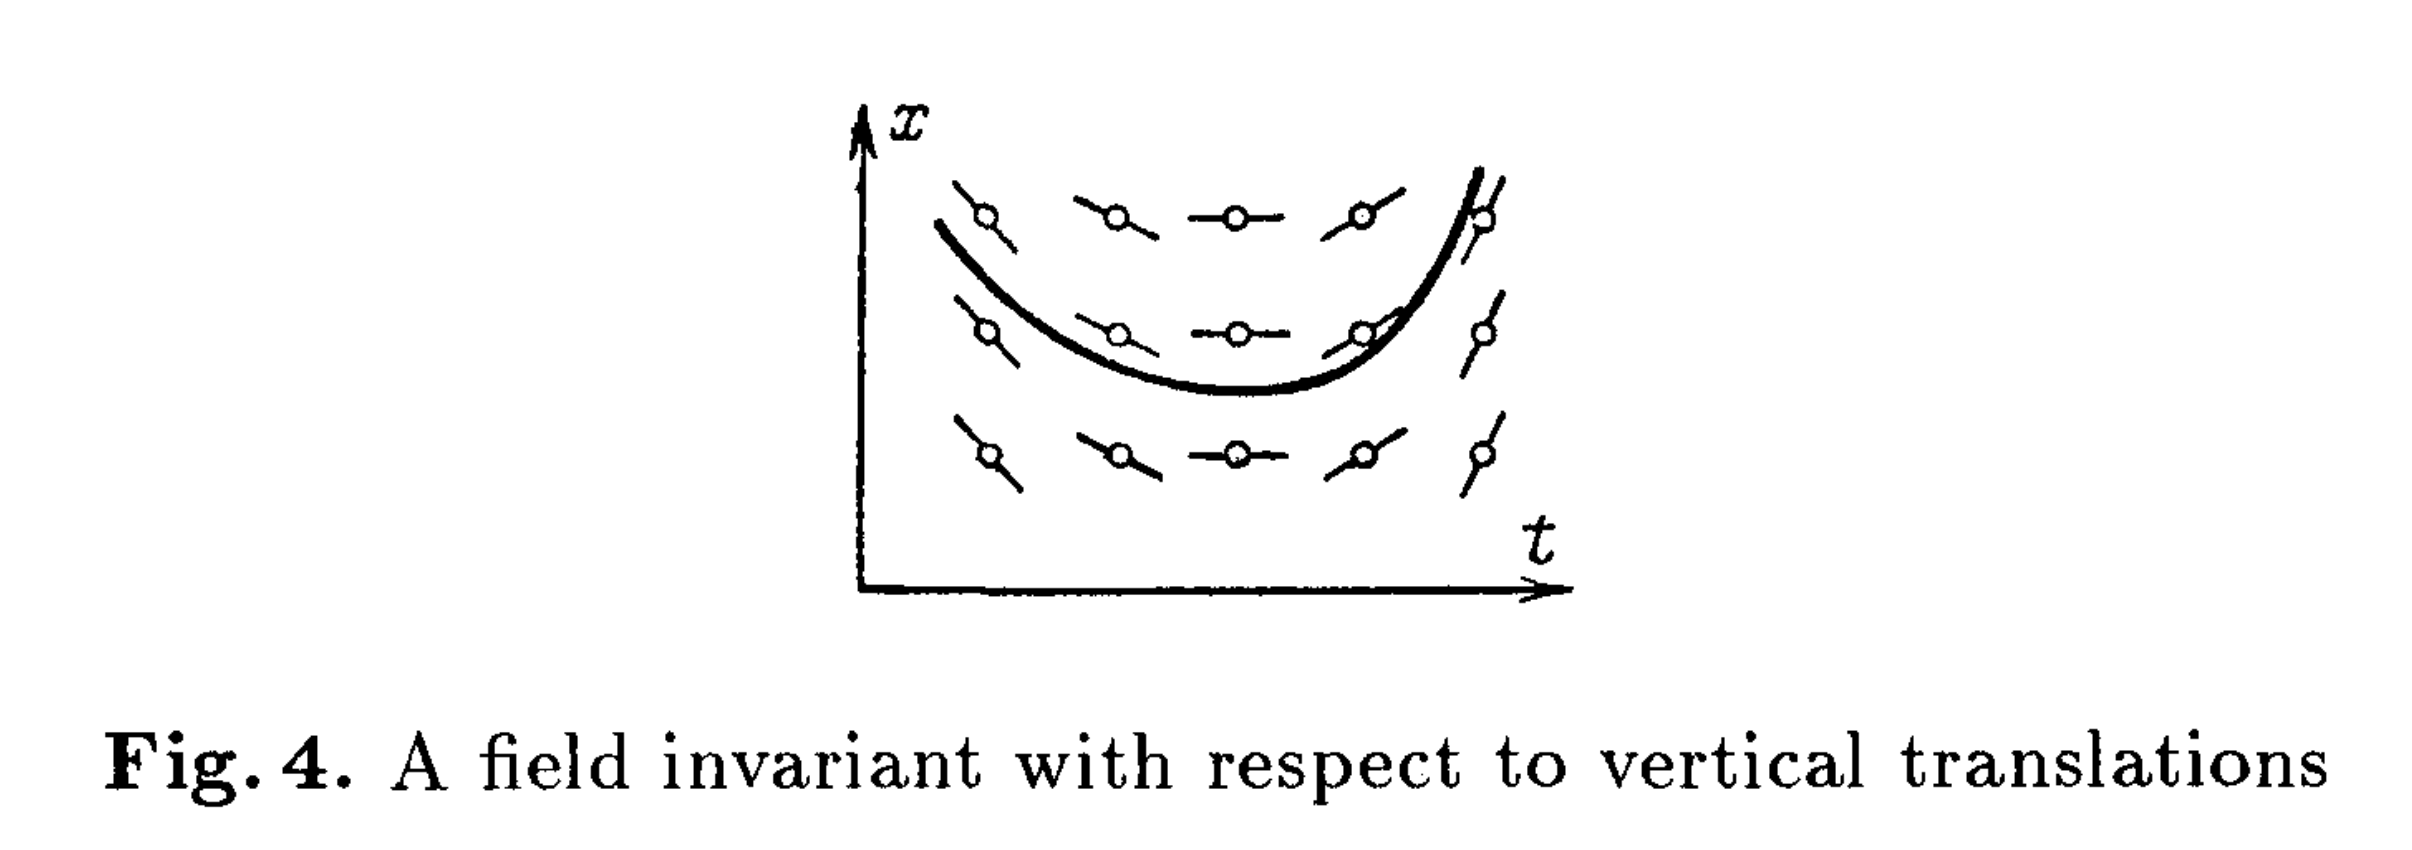
\includegraphics[width=340pt]{img/differential-equations-1-direction-field.png}\\
To find functions that solves this, one possibility is that we can find the
antiderivative explicitly:
\begin{align*}
  \int \dydt \dt := y(t) + C = \int v(t) \dt.
\end{align*}


\subsection{Velocity depends on location only (autonomous)}
\begin{align*}
  \dydt = v(y)
\end{align*}
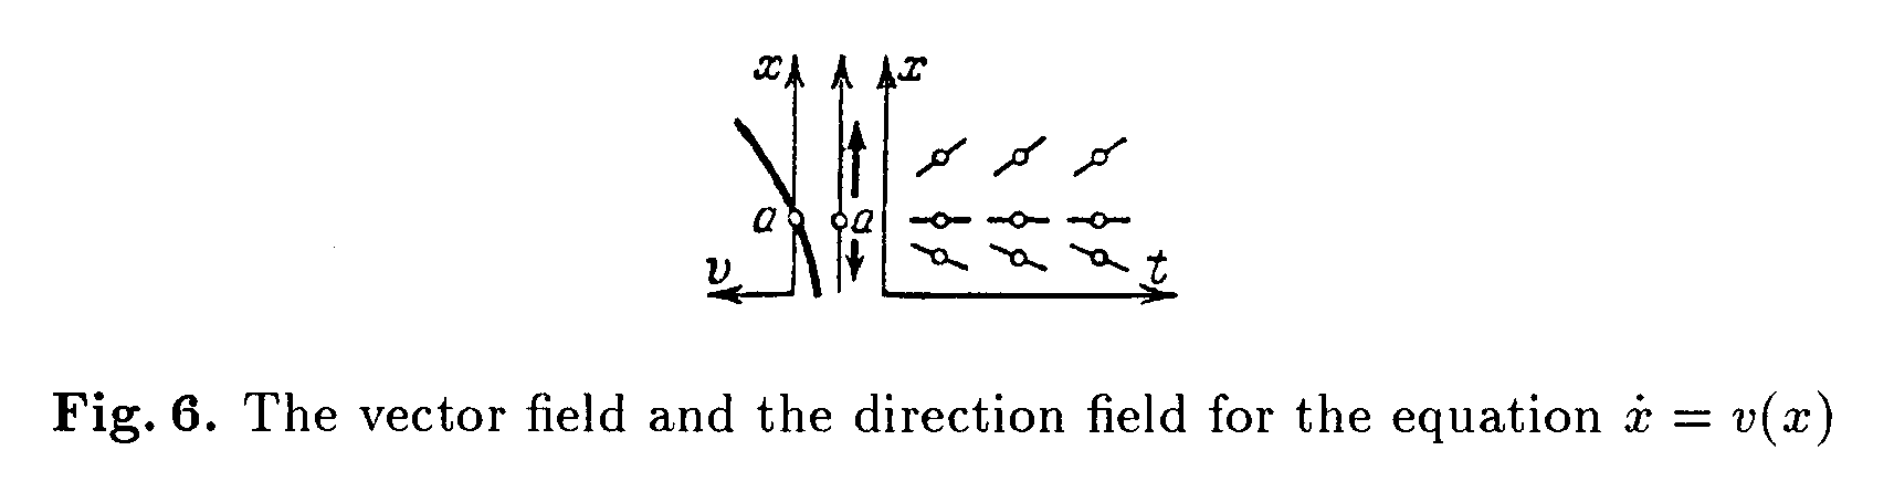
\includegraphics[width=400pt]{img/differential-equations-2-direction-field.png}\\



\section{Examples}
\subsection{C$^{14}$ dating}
\begin{mdframed}
  In a living organism the amount of C$^{14}$, as a proportion of all the
  C$^{12}$ and C$^{14}$, is expected to be a known constant $p_0$. After death,
  C$^{14}$ decays to C$^{12}$. How old is a specimen with proportion $p_1$ of
  C$^{14}$?
\end{mdframed}
Let $\lambda$ be the rate at which one atom of C$^{14}$ decays in atoms/sec. So
in a sample of $N$ atoms, the expected number to decay in one second is
$N\lambda$.

Let $N(t)$ be the number of C$^{14}$ atoms remaining at time $t$. We can
specify the model as a first-order ODE:
\begin{align*}
\frac{\d N}{\dt} = -N\lambda.
\end{align*}
Equivalently, dividing by the constant total number of carbon atoms,
\begin{align*}
\frac{\d p}{\dt} = -p\lambda,
\end{align*}
where $p(t)$ is the proportion of C$^{14}$ at time $t$.

It's easy to find a family of functions $p(t)$ that satisfies this differential equation. Since
\begin{align*}
  \frac{1}{p(t)} \frac{\d p}{\dt} = -\lambda,
\end{align*}
it must be the case that their antiderivatives are the same, up to a constant:
\begin{align*}
  \log(p(t)) &= -\lambda t + C\\
  p(t)  &= Ae^{-\lambda t}.
\end{align*}
Further, the expected proportion in a living organism determines a particular
function as the solution:
\begin{align*}
  p(0) = p_0 = Ae^{-\lambda . 0}
\end{align*}
so $A = p_0$ and the solution is
\begin{align*}
  p(t)  &= p_0e^{-\lambda t}.
\end{align*}
So the estimated age of a sample with proportion $p_1$ is
\begin{align*}
  t = \frac{1}{\lambda}\log\(\frac{p_0}{p_1}\).
\end{align*}



\section{Picard's Existence Theorem}
Consider again the initial value problem
\begin{align*}
  \dydt = v(t, y) ~~~~~~~~~~ y(t_0) = y_0.
\end{align*}


The ODE could also be written as
\begin{align*}
  y(t) = \int v\Big(t, y(t)\Big) \dt + C,
\end{align*}
but this is merely an equivalent restatement, since the definition of
indefinite integral is antiderivative. If we can find an antiderivative, then
fine. If not, note that by FTC, the following definite integral describes a
solution:
\begin{align*}
  y(t) = y(t_0) + \int_{t_0}^t v\Big(\tau, y(\tau)\Big) \d\tau.
\end{align*}
But this specifies $y(t)$ in terms of itself, since the velocity $v$ depends
not only on $t$ but also on the current position\footnote{for example, the rate
  of change of the proportion on carbon-14 depends on the current proportion of
  carbon-14.}.\\

\subsection{Definition: Lipschitz condition}
$v(t, y)$ is Lipschitz in the $y$ direction if there exists an upper bound $L$
on the absolute value of the straight line slope between any two points lying
on a vertical line. I.e. $\exists L > 0$ such that
\begin{align*}
  \Big|v(t, y_1) - v(t, y_0)\Big| \leq L\Big|y_1 - y_0\Big|
\end{align*}
for all pairs of points $(t, y_0)$, $v(t, y_1)$.

\subsection{Theorem: Picard's existence theorem}
\begin{mdframed}
Let $R$ be a rectangle of width $2h$ and height $2k$ and let
$(t_0, y_0)$ be the center of the rectangle. Suppose
\begin{enumerate}
\item Within $R$, $v(t, y)$ is continuous, with $|v(t, y)| \leq M$
\item $Mh \leq k$
\item Within $R$, $v(t, y)$ is Lipschitz in the $y$ direction, with bound $L$
  on the absolute value of the straight line slope between any two points.
\end{enumerate}

Then the initial value problem
\begin{align*}
  \dydt = v(t, y) ~~~~~~~ y(t_0) = y_0
\end{align*}
has a unique solution in $R$.
\end{mdframed}

\subsection{Examples}

In these cases, $|y'|$ and $\partiald{v}{y}$ are bounded in any rectangle.

\subsubsection{A}
$y' = v(x, y) = x^2 + y^2 ~~~~~~~ y(0) = 0$

So it can be approximated by Picard iterates. Is an explicit solution possible here?

\subsubsection{B}
$y' = (1 - 2x)y ~~~~~~~ y(0) = 1$

This can be solved explicitly by separation-of-variables:
\begin{align*}
  \log(y) &= x- x^2 + C\\
  y       &= Ae^{x(1-x)}.
\end{align*}


\subsection{Non-examples}

$|y'|$ is bounded in any rectangle for all these examples. However,
$\partiald{v}{y}$ is not. Picard's theorem guarantees unique solutions only in
rectangles excluding such problematic points.

\subsubsection{A}
$y' = v(x, y) = 3y^{2/3}  ~~~~~~~ y(0) = 0$

$\partiald{v}{y} = 2y^{-1/3} \to \pm \infty$ at $y=0$.


\subsubsection{B}
$y' = v(x, y) = x^2y^{1/5} ~~~~~~~ y(0) = b$

$\partiald{v}{y} = \frac{1}{5}x^2y^{-4/5}$ which is not defined at $y=0$.

\subsubsection{C}
$y' = v(x, y) = y^2       ~~~~~~~ y(0) = 1$

$\partiald{v}{y} = 2y$, so seems like it should be fine. Solve by
separation-of-variables:

\begin{align*}
  \int y^{-2} y' \dx &= x + C\\
  -y^{-1}            &= x + C\\
  y                 &= \frac{1}{C - x}.
\end{align*}
The solution passing through the initial value $y(0) = 1$ is
\begin{align*}
  y                  &= \frac{1}{1 - x},
\end{align*}
which does not exist for all $x$ in the rectangle.


\newpage
\subsection{Proof}

We will show that the following sequence of functions converges to a unique
solution:
\begin{align*}
  y_0(t) &= y_0\\
  y_n(t) &= y_0 + \int_{t_0}^t v\Big(\tau, y_{n-1}(\tau)\Big) \d\tau.\\
\end{align*}

The basic idea is to write the limiting function $y_\infty(t)$ as a telescoping
sum, and then to show that the series thus defined converges.

Define
\begin{align*}
  e_n = y_n - y_{n-1}, ~~~~~~~ n = 1, 2, \ldots.
\end{align*}
Then the limiting function that is our objective is
\begin{align*}
  y_\infty = y_0 + \sum_{n=1}^\infty e_n.
\end{align*}

We need to show
\begin{enumerate}
\item The $y_n(t)$ converge to a function $y(t)$
\item This function is a solution
\item It is unique
\end{enumerate}

\newpage
\subsection{Proof that the $y_n(t)$ converge uniformly to a function $y_\infty(t)$}
We are going to use the Weierstrass M-test to show that the series of functions
converge uniformly. So, we need to show that each $e_n$ is bounded
by some $W_n$, and that the series $\sum_{n=1}^\infty W_n$ converges.

A single term in the series is
\begin{align*}
  e_{n}(t) = \int_{t_0}^t v\Big(\tau, y_{n-1}(\tau)\Big) -
                         v\Big(\tau, y_{n-2}(\tau)\Big) \dt.
\end{align*}

Now, by assumption, $v$ is Lipschitz in the $y$ direction with bound
$L$. (Informally, this means that the absolute value of the straight line slope
between any two points lying on a vertical line is bounded by $L$). Therefore
\begin{align*}
  \Big|v\Big(t, y_{n-1}(t)\Big) -
       v\Big(t, y_{n-2}(t)\Big)\Big| \leq L\Big|y_{n-1}(t) - y_{n-2}(t)\Big|.
\end{align*}
And since $\Big|\int_a^b f(t) \dt\Big| \leq \int_a^b |f(t)| \dt$,
\begin{align*}
  |e_n(t)| \leq L\Big|\int_{t_0}^t \Big|y_{n-1}(\tau) - y_{n-2}(\tau)\Big| \d\tau \Bigg|.
\end{align*}
\footnote{The outer modulus is required to handle the case $t < t_0$.}

For the Weierstrass M-test we need to express the RHS as a constant $W_n$,
depending only on $L, M, n, t_0, y_0$. We will do this by induction.

\newpage
Recall that the definition of the $e_n$ is
\begin{align*}
  e_n(t) := y_n(t) - y_{n-1}(t).
\end{align*}

For the first few terms we have
\begin{align*}
  |e_1(t)| &    = \int_{t_0}^t v(\tau, y_0) \d\tau\\
           & \leq M(t - t_0) \leq Mh\\
  |e_2(t)| & \leq L\int_{t_0}^t \Big|y_1(\tau) - y_0(\tau)\Big| \d\tau\\
           &    = L\int_{t_0}^t |e_1(\tau)| \d\tau\\
           & \leq L\int_{t_0}^t M(\tau - t_0) \d\tau\\
           &    = LM\frac{(\tau - t_0)^2}{2} \Big|_{t_0}^t \\
           &    = LM\frac{(t - t_0)^2}{2} \\
  |e_3(t)| & \leq L\int_{t_0}^t \Big|y_2(\tau) - y_1(\tau)\Big| \d\tau\\
           &    = L\int_{t_0}^t |e_2(\tau)| \d\tau\\
           & \leq L\int_{t_0}^t LM\frac{(t - t_0)^2}{2} \d\tau\\
           &    = L^2M\frac{(t - t_0)^3}{3!}
\end{align*}
So it seems that $|e_n(t)| \leq L^{n-1}M\frac{h^n}{n!}$. To prove this, note that we know
it is true of $e_1$. So suppose it is true of $e_n$. Then the next term is
\begin{align*}
  e_{n+1}(t) &   := y_{n+1}(t) - y_n(t)\\
            & \leq L\int_{t_0}^t \Big|y_n(\tau) - y_{n-1}(\tau)\Big| \d\tau\\
            &=     L\int_{t_0}^t |e_n(\tau)| \d\tau\\
            &=     L\int_{t_0}^t L^{n-1}M\frac{(\tau - t_0)^n}{n!} \d\tau\\
            &=     L^nM\frac{(t - t_0)^{n+1}}{(n+1)!^{~~~}}\\
            & \leq L^nM\frac{h^{n+1}}{(n+1)!},
\end{align*}
so $|e_n(t)| \leq L^{n-1}M\frac{h^n}{n!}$ for all $n \geq 1$ by induction.

Recall that our aim is to show that the Weierstrass M-test series
$\sum_{n=0}^\infty W_n = L^{n-1}M\frac{h^n}{n!}$ converges.

\subsection{Proof that $y_\infty(t)$ is a solution}

To prove that the limiting function $y_\infty$ is a solution, we could either

\begin{enumerate}
\item show that $y'_\infty$
\end{enumerate}

\newpage
\section{Simmons}

\subsection{Picard's theorem}
For every point $(t, y)$ in a rectangle, the ODE
\begin{align*}
  \dydt = f(t, y)
\end{align*}
has a solution passing through that point if $\partiald{f}{y}$ is Lipschitz
continuous in that rectangle.

\subsection{Families of curves}
For a family of curves, say the family of circles
\begin{align}
  x^2 + y^2 = c^2 \label{simmons-circles}
\end{align}
we can obtain a differential equation by implicit differentiation:
\begin{align}
  2x + 2y\dydx = 0. \label{simmons-circles-de}
\end{align}
Alternatively (eoc),
\begin{align*}
  (x + \dx)^2 + (y + \dy)^2 &= c^2\\
  x^2 + 2x\dx + y^2 + 2y\dy &= c^2\\
        2x\dx  + 2y\dy     &= 0.
\end{align*}

\subsection{Orthogonal trajectories}
What's the family of curves each of which is equal to every circle in \eqref{simmons-circles}?

Well, we know that their gradients are negative the inverse of the circle
gradients. So if we let $\dydx$ now be the gradient of the orthogonal
trajectories, then from \eqref{simmons-circles-de},
\begin{align*}
  2x - 2y\dxdy = 0
\end{align*}
is an ODE specifying the family of orthogonal trajectories. Thus
\begin{align*}
  \dydx &= \frac{y}{x}\\
  \log(y) &= \log(x) + C\\
       y &= Ax,
\end{align*}
so the orthogonal trajectories are lines through the origin, as expected.

\subsection{Use of polar coordinates to make a problem tractable (separable)}
TODO

\section{Arnold - Problems}
\subsection{}
\begin{mdframed}
  At what altitude is the density of the air one half of that at the surface of
  the Earth? Regard temperature as constant. One cubic meter of air at the
  Earth's surface weighs 1250g.
\end{mdframed}
\begin{align*}
  \rho(0) = 1250\\
  &=
\end{align*}

\chapter{Complex Analysis - Berkeley Math 185 - Complex Function Theory (Sarason)}
\documentclass[12pt]{article}
\usepackage{fullpage,amsfonts,amsmath,mathpazo,graphicx,verbatim,parskip}
\usepackage[left=2cm,top=2cm,right=2cm,bottom=2cm,head=2cm,foot=1cm]{geometry}
\usepackage{notes}

\renewcommand{\bar}{\overline}

\begin{document}

\begin{center}
  \section*{
    Math 185 - Complex Analysis\\
    Sarason - Complex Function Theory\\
  }
\end{center}
\begin{center}
  \small{
    Dan Davison\\
    \texttt{dandavison7@gmail.com}
  }
\end{center}

\section*{I. Complex Numbers}

\begin{description}

% \begin{comment}

\exercise{I.2.1}{Prove that $\C$ obeys the associative law for multiplication
    and the distributive law.}

  Let $u, v, w \in \C$ with $u = a + bi$, $v = c + di$, and $w = f + gi$.

  Multiplication is associative since
  \begin{align*}
    uv &= (ac - bd) - (ad + bc)i \\
       &= (ca - db) - (cb + da)i = vu. \\
  \end{align*}

  Multiplication is left-distributive over addition since
  \begin{align*}
    u(v + w)
    &= (a + bi)\big((c + f) + (d + g)i\big) \\
    &= (ac + af - bd - bg) + (ad + ag + bc + bf)i \\
    &= (ac - bd) + (ad + bc)i + (af - bg) + (ag + bf)i \\
    &= (a + bi)(c + di) + (a + bi)(f + gi) \\
    &=uv + uw.
  \end{align*}

  Since multiplication is commutative, multiplication is also right-distributive over addition.

\exercise{I.2.2}{Find the multiplicative inverses of the complex numbers (0, 1) and (1, 1)}

\exercise{I.2.3}{Think of $\C$ as a vector space over $\R$. Let $c = (a,b)$ be
  in $\C$, and regard multiplication by $c$ as a real linear transformation
  $T_c$. Find the matrix $M_c$ for $T_c$ with respect to the basis
  $(1, 0), (0, 1)$. Observe that the map $c \mapsto M_c$ preserves addition and
  multiplication. Conclude that the algebra of two-by-two matrices over $\R$
  contains a replica of $\C$.}

  Background:

  What does ``$\C$ as a vector space over $\R$'' mean? A vector space is a set of
  tuples. The elements of the tuples are elements of the field ($\R$ in this
  case). Vector spaces support addition and scalar multiplication, where the
  scalars come from the field. So this means that $\C$ is a set of ordered pairs
  of reals, supporting addition of pairs and multiplication of a pair by a real
  scalar. What it does \textit{not} imply is that pairs can be multiplied,
  although, in the case of $\C$, they can, since $\C$ is a field.

  A linear transformation is a function from one vector space $U$ to another,
  $W$, such that $f(u + w) = f(u) + f(w)$, and $f(au) = af(u)$ for $u \in U$,
  $w \in W$ and $a$ in the field. In other words, the linear transformation
  preserves the two vector space operations, addition and scalar multiplication;
  it is a homomorphism on the vector space.

  OK, so the operation that was ignored by conceiving of $\C$ as a vector space
  over $\R$, multiplication of the vectors, we're going to regard as a ``real
  linear transformation'', i.e. a function of $\R^2$. Find the matrix for it with
  respect to the basis $((1, 0), (0, 1))$. The first basis vector ($1$) is
  transformed as $(1, 0) \mapsto (a, b)(1, 0) = (a, b)$. The second basis vector
  ($i$) is transformed as $(0, 1) \mapsto (a, b)(0, 1) = (-b, a)$. Therefore the
  matrix of $T_c$ is
  $$M_c = \mat{a}{-b}
              {b}{a},$$
  which is a rotation + scaling transformation of $\R^2$.

  \textbf{Observe that the map $c \mapsto M_c$ preserves addition and
    multiplication.}

  Let $f: \R^2 \rightarrow \text{(2x2 matrices)}$ denote the map $c \mapsto M_c$. Then
  $$f(c_1 + c_2) = \mat{a_1 + a_2}{-b_1 - b_2}
                       {b_1 + b_2}{a_1 + a_2} = f(c_1) + f(c_2),$$
  and
  $$f(c_1c_2) = \mat{a_1b_1 - a_2b_2}{-a_1b_2 - a_2b_1}
                    {a_1b_2 + a_2b_1}{a_1b_1 - a_2b_2},$$
  while
  $$f(c_1)f(c_2)
  = \mat{a_1}{-b_1}
        {b_1}{a_1} \mat{a_2}{-b_2}
                       {b_2}{a_2}
  = \mat{a_1a_2 - b_1b_2}{-a_1b_2 - a_2b_1}
        {a_2b_1 + a_1b_2}{a_1a_2-b_1b_2}
  $$

  ? That's not preserving multiplication of complex vectors. Does it mean
  preserving scalar multiplication?

  \textbf{Conclude that the algebra of two-by-two matrices over $\R$
    contains a replica of $\C$}

  The ``algebra of two-by-two matrices over $\R$'' refers to the fact that $2x2$
  matrices can be added, and multiplied by a scalar from the field $\R$ (they
  form a vector space), and can also be multiplied.

% \end{comment}

\exercise{I.4.3}{Prove that if a polynomial with real coefficients has the
    complex root $z$, then it also has $\bar z$ as a root.}

  Let $P:\C \rightarrow \C$ defined by $P(c) = r_0 + r_1c^1 + \ldots + r_kc^k$ be a $k$-th degree
  polynomial of a complex variable $c$, with real coefficients $r_k$, and let
  $z = a + bi$ be a root, i.e. $P(z) = 0$. The claim is that
  $P(\bar z) = 0$.

  To show this, take the complex conjugate of both sides of the equation
  $P(z) = 0$:

  $$
  \bar{P(z)} = \bar{r_0 + r_1z^1 + \ldots + r_kz^k} = \bar 0.
  $$

  Then, since $\bar{z_1 + z_2} = \bar z_1 + \bar z_2$ and $\bar{rz} = r\bar{z}$,

  $$
  r_0 + r_1\bar{z^1} + \ldots + r_k\bar{z^k} = P(\bar z) = 0,
  $$

  proving that if $z$ is a root then $\bar z$ is a root also.

\exercise{I.7.4}{Prove that the distinct complex numbers $z_1, z_2, z_3$ are
  the vertices of an equilateral triangle if and only if
  $$z_1^2 + z_2^2 + z_3^2 = z_1z_2 + z_2z_3 + z_3z_1$$}

  The condition can be rewritten as
  $$
  (z_1 - z_2)^2 + (z_2 - z_3)^2 + (z_3 - z_1)^2 = 0,
  $$
  Each of the three terms on the left side is the square of a complex number
  which, when viewed as a vector in $\R^2$, forms one side of a triangle.

  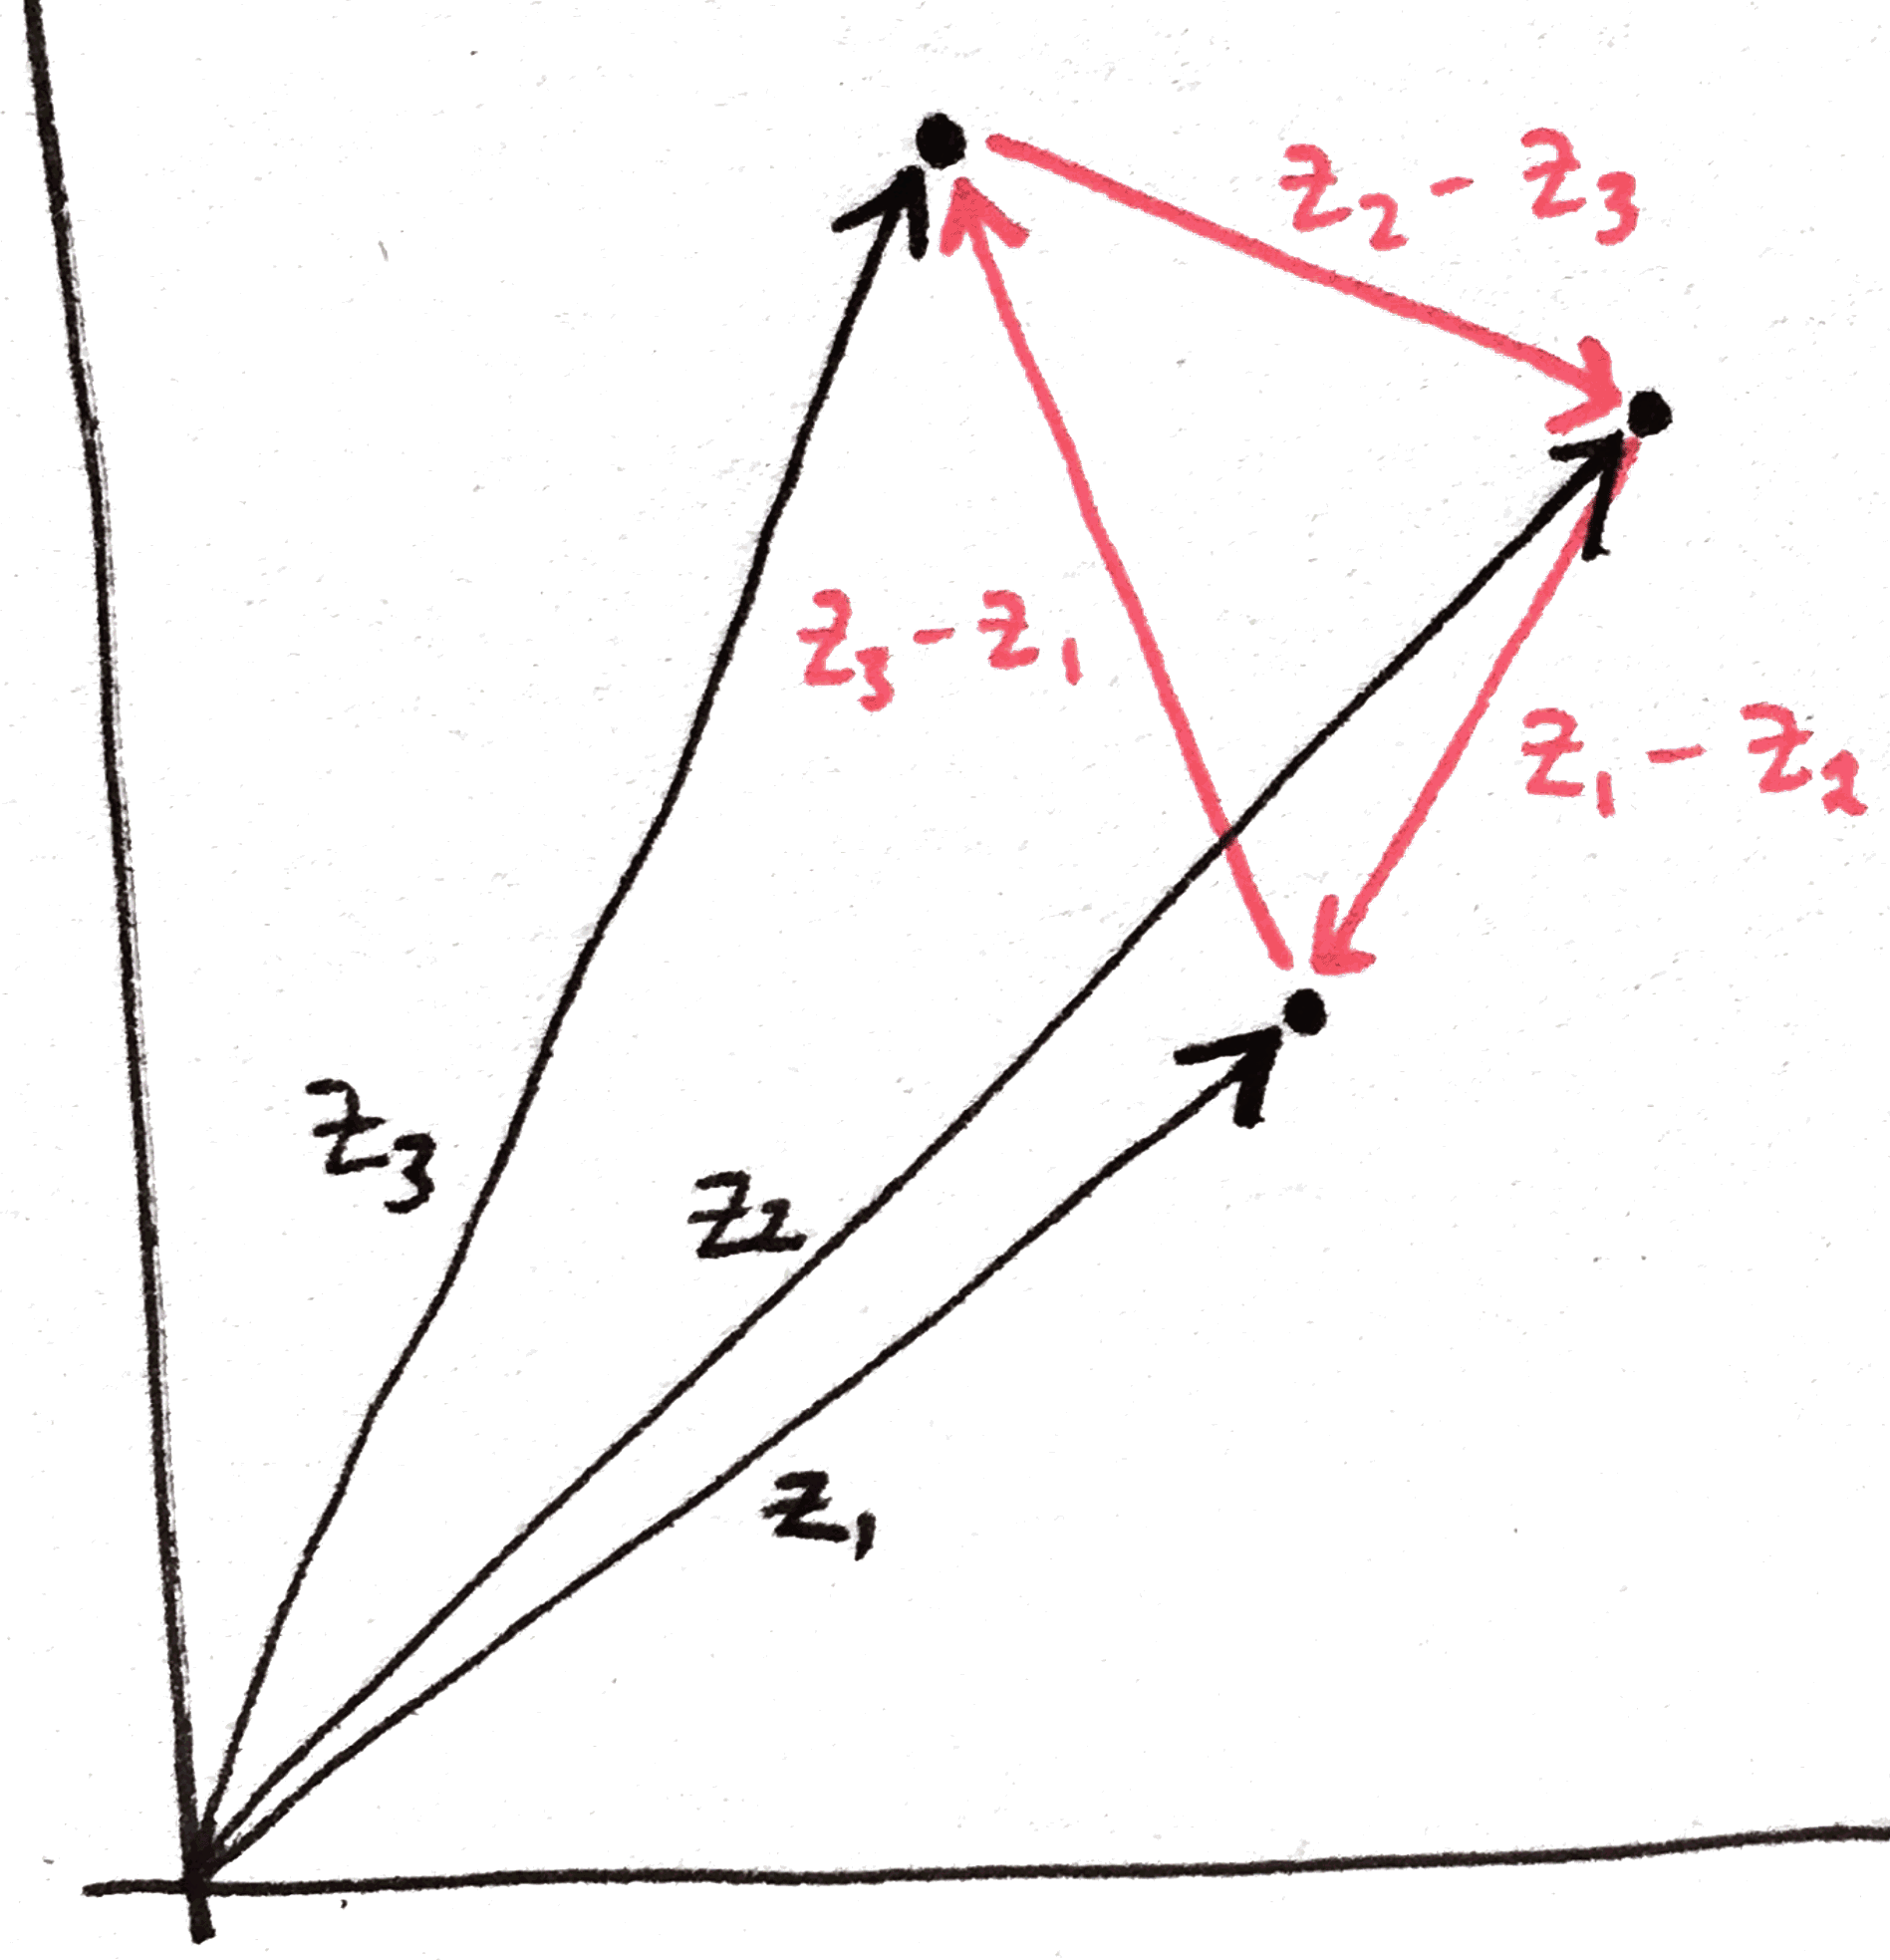
\includegraphics[width=100pt]{img/equilateral-1.png}

  So the original claim is equivalent to the claim that the three vectors
  $$
  (z_1 - z_2)^2, ~ (z_2 - z_3)^2, ~ (z_3 - z_1)^2
  $$
  sum to 0 if and only if the triangle is equilateral.

  First let's prove that if the triangle is equilateral, then the three vectors
  sum to 0. Translate each of the unsquared vectors
  $$
  (z_1 - z_2), ~ (z_2 - z_3), ~ (z_3 - z_1)
  $$
  so that they originate at the origin; they are of equal magnitude and they
  divide the circle into 3 sectors of equal angle $\frac{2\pi}{3}$. Let
  $\theta < \frac{2\pi}{3}$ be the arbitrary angle between one of the vectors and
  the first coordinate axis. Interpreted as complex numbers, we see that their
  arguments are $\theta$, $\frac{2\pi}{3} + \theta$, and
  $\frac{4\pi}{3} + \theta$.

  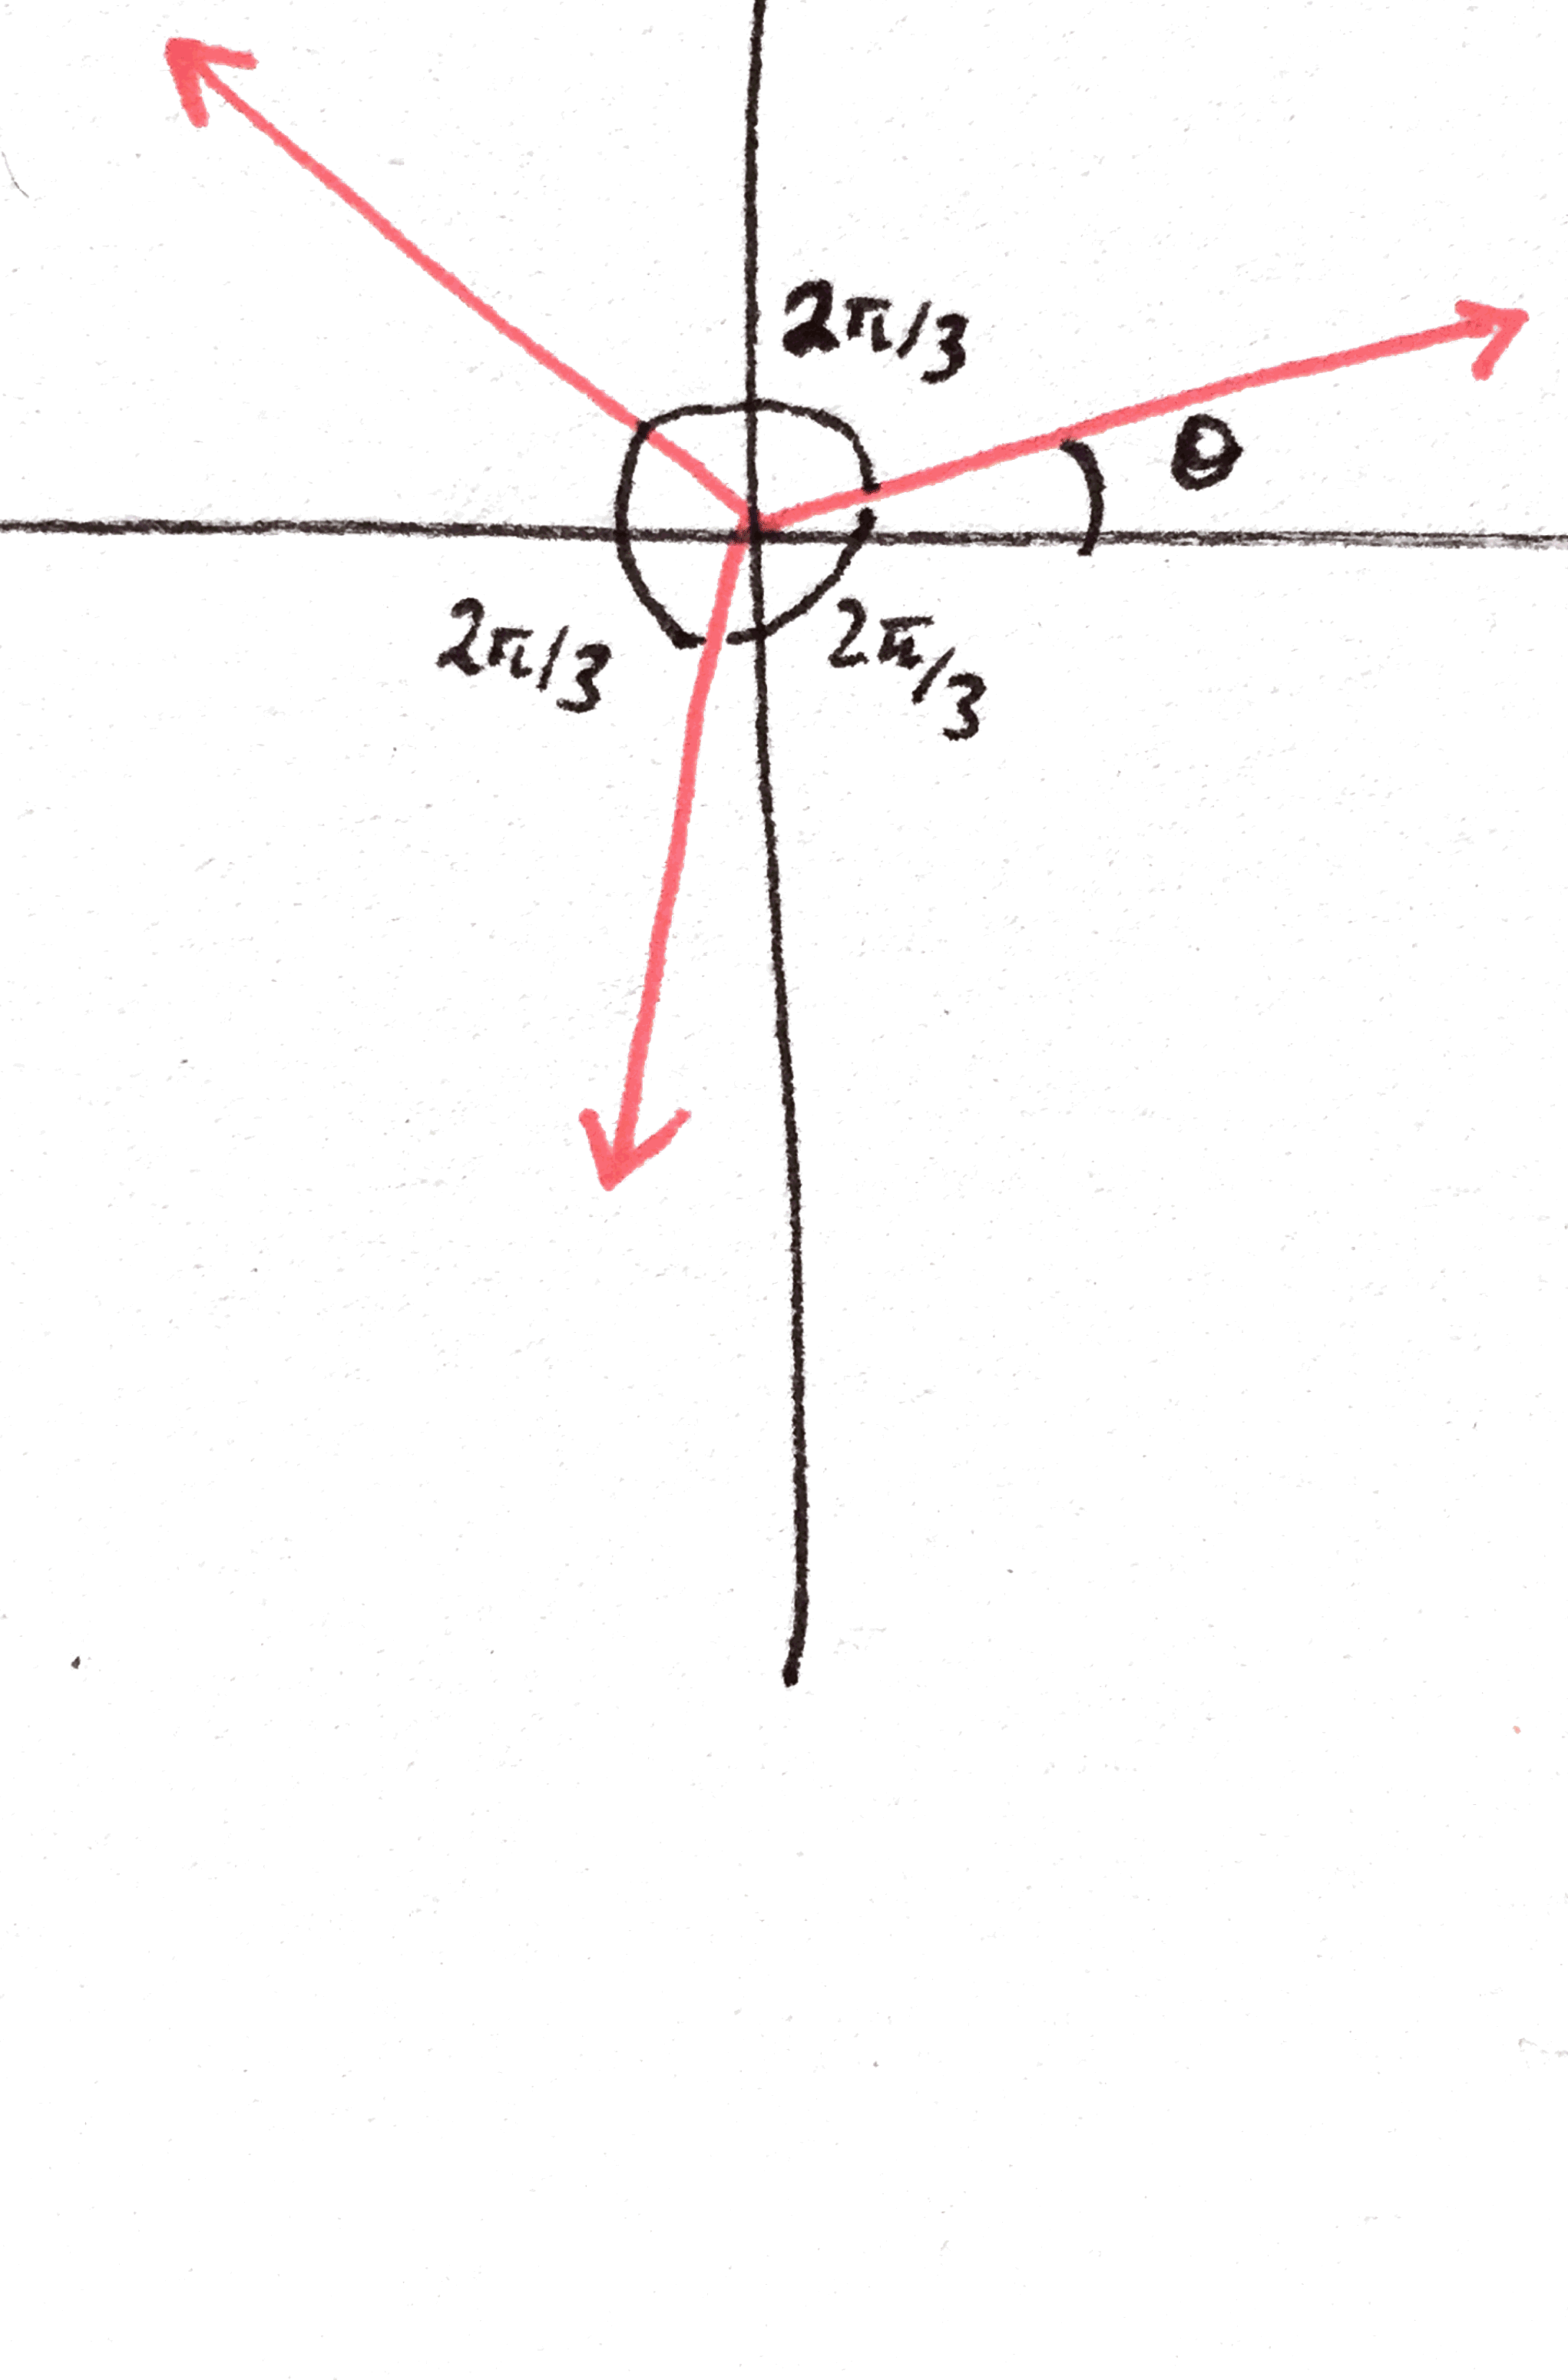
\includegraphics[width=100pt]{img/equilateral-2.png}

  Now we form their squares
  $$
  (z_1 - z_2)^2, ~ (z_2 - z_3)^2, ~ (z_3 - z_1)^2.
  $$
  Since $(z_1 - z_2)$, $(z_2 - z_3)$, and $(z_3 - z_1)$ are of equal magnitude,
  so are their squares. And the arguments of their squares are $2\theta$,
  $\frac{4\pi}{3} + 2\theta$, and
  $\frac{8\pi}{3} + 2\theta \equiv \frac{2\pi}{3} + 2\theta$ mod
  $2\pi$. Therefore the three squared side vectors, when translated so that
  they originate at the origin, also divide up the circle into sectors of equal
  angle $\frac{2\pi}{3}$: the geometrical picture differs from the previous one
  only by a uniform scaling and relabeling of the vectors, and we conclude that
  these squared vectors also sum to zero (return to the origin when placed
  head-to-tail). I.e. the equilaterality assumption implies
  $$
  (z_1 - z_2)^2 + (z_2 - z_3)^2 + (z_3 - z_1)^2 = 0,
  $$
  proving one direction of the equivalence.

  To prove the other direction, we need to show that if
  $$
  z_1^2 + z_2^2 + z_3^2 = z_1z_2 + z_2z_3 + z_3z_1,
  $$
  or equivalently,
  $$
  (z_1 - z_2)^2 + (z_2 - z_3)^2 + (z_3 - z_1)^2 = 0,
  $$
  then the triangle is equilateral. For example, it would suffice to show that
  $$
  |z_1 - z_2| = |z_2 - z_3| = |z_3 - z_1|,
  $$
  but I haven't found a way to do so.

  % The left side of this equation obeys the following triangle inequality
  % $$
  % |z_1^2 + z_2^2 + z_3^2|
  % \le |z_1|^2 + |z_2|^2 + |z_3|^2,
  % $$
  % and the right side obeys
  % $$
  % |z_1z_2 + z_2z_3 + z_3z_1|
  % \le |z_1||z_2| + |z_2||z_3| + |z_3||z_1|.
  % $$

\exercise{I.10.1}{Use de Moivre's formula to find expressions for
  $\cos 5\theta$ and $\sin 5\theta$ as polynomials in $\cos \theta$ and
  $\sin \theta$.}

  From de Moivre's formula we have
  $(\cos\theta + i\sin\theta)^5 = \cos 5\theta + i\sin 5\theta$. The left hand
  side expands as
  \begin{align*}
  (\cos\theta + i\sin\theta)^5 =& \cos^5\theta \\
                               &+ 5i\cos^4\theta\sin\theta \\
                               &- 10\cos^3\theta\sin^2\theta \\
                               &- 10i\cos^2\theta\sin^3\theta \\
                               &+ 5\cos\theta\sin^4\theta \\
                               &+ i\sin^5\theta.
  \end{align*}
  Equating real and imaginary components from the right side and the expansion of
  the left side we have
  \begin{align*}
  \cos 5\theta &= \cos^5\theta - 10\cos^3\theta\sin^2\theta + 5\cos\theta\sin^4\theta \\
  \sin 5\theta &= \sin^5\theta - 10\cos^2\theta\sin^3\theta + 5\cos^4\theta\sin\theta
  \end{align*}
  We can write these as polynomials in $\cos\theta$ and $\sin\theta$
  respectively by using the identity $\cos^2\theta = 1 - \sin^2\theta$:
  \begin{align*}
  \cos 5\theta
  &= \cos^5\theta - 10\cos^3\theta(1 - \cos^2\theta) + 5\cos\theta(1 - 2\cos^2\theta + \cos^4\theta) \\
  &= 16\cos^5\theta - 20\cos^3\theta + 5\cos\theta, \\
  \sin 5\theta
  &= \sin^5\theta - 10(1 - \sin^2\theta)\sin^3\theta + 5(1 - 2\sin^2\theta + \sin^4\theta)\sin\theta \\
  &= 16\sin^5\theta - 20\sin^3\theta + 5\sin\theta.
  \end{align*}

\exercise{I.11.4}{Prove that the sum of the $n$-th roots of 1 equals 0,
  ($n > 1$).}

Let $w = \cos \frac{2\pi}{n} + i\sin \frac{2\pi}{n}$ be the $n$-th root of 1
with smallest argument, other than 1 itself. Then the sum of the roots is
$1 + w + w^2 + \ldots + w^{n-1}$. This is the first $n$ terms of a geometric
series with constant ratio $w$, and is therefore equal to
$\frac{1 - w^{n}}{1 - w} = \frac{1 - 1}{1 - w} = 0$.


\exercise{I.11.5}{Let $w$ be an $n$-th root of 1 different from 1
  itself. Establish the formulas
  $$
  1 + 2w + 3w^2 + \ldots + nw^{n-1} = \frac{n}{w -1},
  $$
  $$
  1 + 4w + 9w^2 + \ldots + n^2w^{n-1} = \frac{n^2}{w-1} - \frac{2n}{(w-1)^2}.
  $$
}

  [Note: my answers to this question appear to be wrong.]

  The sum of the first $n+1$ terms of a geometric series with first term $1$ and
  constant ratio $w$ is

  $$
  1 + w + w^2 + \ldots + w^{n} = \frac{~~~~~1 - w^{n+1}}{1 - w} = \frac{1 - w}{1 - w} = 1,
  $$
  since $w^{n+1} = w$.

  Taking derivatives of both sides gives
  $$
  1 + 2w + 3w^2 + \ldots + nw^{n-1} = 0,
  $$

  which does not agree with the given formula, so something's wrong.

  Nevertheless, if it were the case that
  $$
  1 + 2w + 3w^2 + \ldots + nw^{n-1} = \frac{n}{w -1}
  $$
  then we could multiply by $w$, giving
  $$
  w + 2w^2 + 3w^3 + \ldots + nw^n = \frac{nw}{w -1},
  $$
  and differentiate with respect to $w$ again, giving
  $$
  1 + 4w + 9w^2 + \ldots + n^2w^{n-1} = \frac{(w-1)n - nw}{(w - 1)^2} = \frac{n}{w - 1} - \frac{nw}{(w - 1)^2},
  $$
  which also doesn't agree with the given formula.


% \begin{comment}

\exercise{I.13.1}{Stereographic projection}

  The stereographic projection maps $z$ onto the surface of a sphere according to
  $$
  z \mapsto \frac{(2 \Re z, 2 \Im z, |z|^2 - 1)}{|z|^2 + 1}.
  $$
  % It's 1-1 and the inverse map is
  % $$
  % (\xi, \eta, \zeta) \mapsto (s + 1)\frac{\xi}{2} + (s + 1)\frac{\eta}{2}i
  % $$

\exercise{I.13.1}{Establish the following formula for the spherical metric
$$
\rho(z_1, z_2) = \frac{2|z_1 - z_2|}{\sqrt{|z_1|^2 + 1}\sqrt{|z_2|^2 + 1}}
$$}

  $\rho(z_1, z_2)$
  is the Euclidean distance between the image points of $z_1$ and $z_2$ on the
  Riemann sphere, therefore
  \begin{align*}
  \rho(z_1, z_2)
  &=
  \left|
  \frac{(2 \Re z_1, 2 \Im z_1, |z_1|^2 - 1)}{|z_1|^2 + 1} -
  \frac{(2 \Re z_2, 2 \Im z_2, |z_2|^2 - 1)}{|z_2|^2 + 1}
  \right| \\
  &=
  \left|
  \frac{
  (2 \Re z_1, 2 \Im z_1, |z_1|^2 - 1)(|z_2|^2 + 1) -
  (2 \Re z_2, 2 \Im z_2, |z_2|^2 - 1)(|z_1|^2 + 1)
  }
  {(|z_1|^2 + 1)(|z_2|^2 + 1)}
  \right| \\
  \end{align*}
  Meanwhile,
  $$
  |z_1 - z_2| = \sqrt{(\Re z_1 - \Re z_2)^2 + (\Im z_1 - \Im z_2)^2}
  $$

% \end{comment}

\exercise{I.14.1}{Establish the formula
$$
\rho(z, \infty) = \frac{2}{\sqrt{|z|^2 + 1}}
$$
}

  $\rho(z, \infty)$ is the Euclidean distance between the image point of $z$ and
  the north pole $(0, 0, 1)$:
  \begin{align*}
  \rho(z, \infty)
  &= \sqrt{
  \(\frac{2 \Re z}{|z|^2 + 1} - 0\)^2 +
  \(\frac{2 \Im z}{|z|^2 + 1} - 0\)^2 +
  \(\frac{|z|^2 - 1}{|z|^2 + 1} - 1\)^2
  } \\
  &= \frac
  {\sqrt{4 \(\Re z\)^2 + 4 \(\Im z\)^2 + 4}}
  {|z|^2 + 1} \\
  &= \frac
  {2}
  {\sqrt{|z|^2 + 1}}.
  \end{align*}

\end{description}

\section*{II. Complex Differentiation}

Consider $z$ approaching $z_0$. $z - z_0$ is a vector pointing from $z_0$ to
$z$, and $f(z) - f(z_0)$ is a vector pointing between the image points for some
complex-valued function $f$. The derivative of $f$ at $z_0$ is the rotation +
scaling linear transformation (i.e. the complex number $c$) that takes
$z - z_0$ as close as possible to $f(z) - f(z_0)$. Note that the transformation
must be the \textit{same} regardless of the path taken by $z$ as it approaches
$z_0$. In other words, the action of $f$ on \textit{all} vectors in an
infinitisimal disc around $z_0$ is the same as multiplying by a complex number
$c$.

The transformation $f$ can be described by two surfaces over the complex plane:
$u(x,y)$ and $v(x,y)$, so that $f: \cvec{x}{y} \mapsto
\cvec{u(x,y)}{v(x,y)}$. If $f$ is differentiable at $(x_0, y_0)$ then it has a
local linear approximation with sublinear error. That linear approximation is
$$
\cvec{u(x, y)}
     {v(x, y)} \approx \cvec{u(x_0, y_0)}
                            {v(x_0, y_0)} + \cvec{(x - x_0)\dudx + (y - y_0)\dudy}
                                                 {(x - x_0)\dvdx + (y - y_0)\dvdy}
$$
This is more succinctly expressed using the Jacobian:
$$
\cvec{u(x, y)}
     {v(x, y)} \approx \cvec{u(x_0, y_0)}
                            {v(x_0, y_0)} + \mat{u_x}{u_y}
                                                {v_x}{v_y} \cvec{x - x_0}
                                                                {y - y_0}.
$$
Note that this "linear approximation" form
$$
y \approx y_0 + y'(x - x_0)
$$
could just as well be written
$$
y - y_0 \approx y'(x - x_0)
$$
showing that one way of describing the derivative is "whatever you have to
multiply a small displacement in the input space by to get the displacement in
the output space".

Recall that the derivative of a complex function $f$ is defined to be a complex
number,
$$
f'\(\cvec{x_0}
        {y_0}\) = \lim_{(x,y) \rightarrow (x_0,y_0)}
\frac{
\cvec{u(x, y)}
     {v(x, y)} - \cvec{u(x_0)}
                      {v(y_0)}
}
{
\cvec{x}
     {y} - \cvec{x_0}
                {y_o}.
},
$$
i.e.
$$
f'(z_0) = \lim_{z \rightarrow z_0} \frac{f(z) - f(z_0)}{z - z_0},
$$
i.e. the derivative is whatever complex number you multiply the vector $z-z_0$
by to get its image vector $f(z) - f(z_0)$, in the limit as $z \rightarrow z_0$.

The partial derivatives of the complex-valued $f$ in the real and imaginary
directions are the complex numbers
\begin{align*}
f_x &= u_x + iv_x\\
f_y &= u_y + iv_y\\
\end{align*}
or
\begin{align*}
f_x &= \cvec{u_x}{v_x}\\
f_y &= \cvec{u_y}{v_y}\\
\end{align*}

The geometric interpretation of these is that they define how the image vector
$f(z)$ changes in response to a small change to $z$.

$u$ can be approximated by a local tangent plane. That's what $u_x$ and $v_x$
do. And so can $v$; that's what $v_x$ and $v_y$ do. But when we consider the
effect of a small displacement in the 2D input space on the 2D output space, we
describe the two tangent plane approximations jointly as a linear
transformation of the input plane, defined by the Jacobian. The thing is, the
linear transformation must have the same effect as multiplication by a complex
number.

The derivative is "what you have to multiply the input displacement by to get
the output displacement". That's true for a single-variable function
$\R \rightarrow \R$
$$
u(x) - u(x_0) = f'(x_0) \cdot (x - x_0)
$$
and it's true for a surface over the plane $(\R^2 \rightarrow \R$)
$$
u(x, y) - u(x_0, y_0) = \dudx \cdot (x - x_0) + \dudy \cdot (y - y_0)
$$
so presumably something analogous holds for a linear transformation of the
plane $(\R^2 \rightarrow \R^2$), i.e.
$$
\vec z - \vec z_0 = \dveczdx \cdot (x - x_0) + \dveczdy \cdot (y - y_0).
$$
or
$$
\cvec{u(x, y)}{v(x, y)} - \cvec{u(x_0, y_o)}{v(x_0, y_0)} =
\cvec{u_x}{v_x} \cdot (x - x_0) + \cvec{u_y}{v_y} \cdot (y - y_0).
$$
That's exactly the same as the equation involving the Jacobian above
$$
\cvec{u(x, y)}
     {v(x, y)} - \cvec{u(x_0, y_0)}
                      {v(x_0, y_0)} = \mat{u_x}{u_y}
                                          {v_x}{v_y} \cvec{x - x_0}
                                                          {y - y_0}.
$$

So how are we to make sense of the equation relating $f'$ and the partial
derivatives $\dfdx$ and $\dfdy$? Clearly in some sense the Jacobian \textit{is}
$f'$, or at least, the complex number that does what the Jacobian does is
$f'$. And
\begin{align*}
\dfdx &= \cvec{u_x}
              {v_x} = u_x + iv_x \\
\dfdy &= \cvec{u_y}
              {v_y} = u_y + iv_y,
\end{align*}
and so from the Cauchy-Riemann constraint
\begin{align*}
\dfdy &= -v_x + iu_x = i\dfdx,
\end{align*}
i.e. the partial derivative w.r.t. $y$ points at 90° to the $x$ partial
derivative.

% $f_x$ is the complex number that transforms a small real displacement vector
% $\epsilon$ to its image, and $f_y$ is the complex number that transforms a
% small imaginary displacement vector $i\delta$ to its image. [But shouldn't
% these be the same and equal to $f'$, seeing as $f'$ rotates and scales all
% displacement vectors in an infinitesimal disc uniformly? Instead, C-R says that
% $f_x = -if_y$.]

% One notation for the "directional derivative" of $f$ in the direction of
% $\vec z$ is $\frac{\partial f}{\partial \vec z}$. Is this an entirely separate
% notion from the partial derivatives $\frac{\partial f}{\partial z}$ and
% $\frac{\partial f}{\partial \bar z}$ considered in the context of complex
% analysis / Wirtinger derivatives?

So if the local linear approximation to the transformation $f$ behaves exactly as
multiplication by a complex number, then the Jacobian must have the form of a
rotation+scale matrix, $\smat{a}{-b}
                             {b}{a}$. Therefore the Jacobian must satisfy the
Cauchy-Riemann equations
$$
\begin{cases}
u_x = v_y \\
v_x = -u_y. \\
\end{cases}
$$
The Jacobian that effects the local linear rotation+scale transformation, together with
the equivalent complex number, is
$$
\mat{u_x}{-v_x}
    {v_x}{u_x} ~~~~ u_x + iv_x
$$
or
$$
\mat{v_y}{u_y}
    {-u_y}{v_y} ~~~~ v_y - iu_y.
$$
So we can write
\begin{align*}
f'
&= u_x + iv_x = f_x \\
&= v_y - iu_y = -if_y,
\end{align*}
therefore as above, another expression of the Cauchy-Riemann criterion is
$$
f_x = -if_y.
$$
Question: what is the intuition for the fact that the complex number
representing the partial derivative with respect to $x$ is the \textit{same} as
the complex number that effects the full linear transformation? (and at 90° to
the partial with respect to $y$) And what's the intuition for the fact that
$\dfdz = \dfdx$, while $\dfdzbar = 0$?

% The partial derivatives of the complex-valued $f$ in the real and imaginary
% directions are
% \begin{align*}
% \dfdx &= \dudx + i\dvdx\\
% \dfdy &= \dudy + i\dvdy\\
% \end{align*}

% So we can write
% \begin{align*}
% f'(z_0)
% &= \dudx(z_0) + i \dvdx(z_0) =   \dfdx(z_0) \\
% &= \dvdy(z_0) - i \dudy(z_0) = -i\dfdy(z_0),
% \end{align*}
% or
% \begin{align*}
% f'\(\cvec{x_0}{y_0}\)
% &= \cvec{\dudx(z_0)}{\dvdx(z_0)}  =   \dfdx(z_0)  \\\\
% &= \cvec{\dvdy(z_0)}{-\dudy(z_0)} = -i\dfdy(z_0).
% \end{align*}

$f$ is differentiable iff the error in the linear transformation goes to $0$ as
$(x,y) \rightarrow (x_0,y_0)$ (i.e. real partial derivatives of $u$ and $v$
exist) and the partial derivatives satisfy the Cauchy-Riemann equations.

\subsection*{Partial derivatives in the $z$ and $\bar z$ directions}
The (fixed) $x, y$ and (varying) $z, \bar z$ directions are related by
\begin{align*}
x &= (z + \bar z)/2 \\
y &= (z - \bar z)/2i.
\end{align*}
So by the chain rule,
\begin{align*}
\dfdz
&= \dfdx \dxdz + \dfdy \dydz \\
&= (u_x + iv_x)\frac{1}{2} + i(u_x + iv_x)\frac{1}{2i} \\
&= u_x + iv_x \\
&= \dfdx
\end{align*}
and
\begin{align*}
\dfdzbar
&= \dfdx \dxdzbar + \dfdy \dydzbar \\
&= (u_x + iv_x)\frac{1}{2} + i(u_x + iv_x)\frac{-1}{2i} \\
&= \frac{1}{2}\Big((u_x - u_x) + i(v_x - v_x)\Big) \\
&= 0.
\end{align*}

\begin{description}

\exercise{II.8.1(b,d)}{
  Let the function $f$ be holomorphic in the open disc $D$. Prove that each of
  the following conditions forces $f$ to be constant:\\\\
  \textnormal{Let $f(z) = u(z) + iv(z)$.}
  \begin{description}
    \exercise{(a)}{$f' = 0$ throughout $D$} \\\\
    \textnormal{ \textbfit{Informally:} $f' = 0$ throughout $D$ means that the
      best linear approximation of $f(z) - f(z_0)$ is $0(z - z_0)$ which
      implies that $f(z) = f(z_0)$ everywhere, so $f$ is constant.\\
      ~\\
      \textbfit{Formally:} Since $f$ is holomorphic, $f' = u_x + iv_x =
      0$. Equating real and imaginary parts shows that $u_x = v_x = 0$ and
      therefore that $v_y = u_x = 0$ and $u_y = -v_x = 0$. Since the Jacobian
      of $f$ is the zero matrix, $f$ is constant.}\\
    \exercise{(b)}{$f$ is real-valued in $D$} \\\\
    \textnormal{
      % \textbfit{Informally:}
      $f$ is real-valued, so $f(z) - f(z_0)$ is real-valued. Therefore the
      local linear approximation $c(z - z_0)$ collapses the plane onto the real
      axis, i.e. the Jacobian matrix has the form $\mat{a}{b} {0}{0}$. But $f$
      is holomorphic, so the Jacobian must also have the form
      $\mat{a}{-b}
           {b}{a}$. Therefore the Jacobian is the zero matrix, i.e.
      all partial derivatives are zero, $u_x = u_y = v_x = v_y = 0$, so $f$ is constant.\\
      % \textbfit{Formally:} $f$ is real-valued means that $v(z) = 0$
      % everywhere. Therefore the partial derivatives $v_x = v_y = 0$. Since $f$
      % is holomorphic the partial derivatives satisfy the Cauchy-Riemann
      % equations, therefore we have $u_x = v_y = 0$ and $u_y = -v_x = 0$. The
      % Jacobian is the zero matrix hence $f$ is constant.
      % \\
    }
    \exercise{(c)}{$|f|$ is constant in $D$} \\\\
    \textnormal{ \textbfit{Informally:} $|f|$ is constant means that it collapses
      all points in the open disc $D$ onto a circle. Therefore the Jacobian of
      $f$ has determinant $0 = u_x^2 + v_x^2 = v_y^2 + u_y^2$. Therefore the
      Jacobian
      is the zero matrix and the function $f$ is constant.\\
      ~\\
      \textbfit{Formally:} $|f|$ is constant, therefore
      $|f|^2 = f\bar f = u^2 + v^2$ is constant. Therefore the following two
      partial derivatives are constant:
      \begin{align*}
        \begin{cases}
          \ddx |f|^2 =  2uu_x + 2vv_x = 0 \\
          \ddy |f|^2 = 2uu_y + 2vv_y = 0.
        \end{cases}
      \end{align*}
      Since $f$ is holomorphic, $u_x = v_y$ and $u_y = -v_x$, so
      \begin{align*}
        \begin{cases}
          uu_x - vu_y = 0 \\
          uu_y + vu_x = 0,
        \end{cases}
      \end{align*}
      % i.e.
      % $$
      % \mat{u}{-v}
      %     {u}{v} \cvec{u_x}{u_y} = \cvec{0}{0}.
      % $$
      % The determinant of this system is $2uv$ which is not in general zero. But
      % the equations hold throughout the disc $D$, therefore
      Multiplying the first equation by $u$ and the second by $v$ we have
      $$
      \begin{cases}
        u^2u_x - uvu_y = 0 \\
        uvu_y + v^2u_x = 0,
      \end{cases}
      $$
      and summing these gives
      $$
      u_x(u^2 + v^2) = 0,
      $$
      which proves that either $u_x = 0$ or that $f$ is constant (in which case $u_x = 0$ also).\\
      Similarly, multiplying the first equation by $v$ and the second by $u$ gives
      $$
      \begin{cases}
        uvu_x - v^2u_y = 0 \\
        u^2u_y + uvu_x = 0,
      \end{cases}
      $$
      and subtracting the first from the second gives
      $$
      u_y(u^2 + v^2) = 0.
      $$
      We conclude that $u_x = u_y = 0$ and that $f$ is therefore constant.  }
    \exercise{(d)}{$\arg f$ is constant in $D$} \\\\
    \textnormal{
      %\textbfit{Informally:}
      Let $\arg f = \theta$, constant throughout
      $D$. Then $\arg (f(z) - f(z_0)) = \theta$, whenever $z \neq z_0$.
      Therefore the best local linear approximation to $f$ is a linear
      transformation that collapses the plane onto a line with angle $\theta$.
      The Jacobian determinant is therefore zero. Since $f$
      is holomorphic the Jacobian is of the form $\mat{a}{-b}
                                                      {b}{a}$ and therefore we have
      $a^2 + b^2 = 0$, so $a = b = 0$.  Therefore the Jacobian is the zero
      matrix, i.e. $f' = 0$ throughout $D$, so $f$ is constant.\\
      % ~\\
      % \textbfit{Formally:}
      % The polar form of the Cauchy-Riemann equations is
      % \begin{align*}
      % v_\theta &= ru_r \\
      % u_\theta &= -rv_r.
      % \end{align*}
      % Since $\arg f$ is constant, $v_\theta$
    }
  \end{description}
}

\exercise{II.8.2}{
  Let the function $f$ be holomorphic in the open set $G$. Prove that the
  function $g(z) = \bar{f(\bar z)}$ is holomorphic in the set
  $G^* = \{\bar z: z \in G\}$.
} \\\\
Let
\begin{align*}
f: x + iy &\mapsto s(x, y) + i t(x,y). \\
g: x + iy &\mapsto u(x, y) + i v(x,y) \\
\end{align*}
We want to show that the Jacobian of $g$ exists and and satisfies the
Cauchy-Riemann equations. We have
\begin{align*}
g(x + iy)
&= \bar{s(x, -y) + i t(x, -y)} \\
&= s(x, -y) - i t(x, -y),
\end{align*}
and therefore
\begin{align*}
  u(x,y) &= s(x, -y) \\
  v(x, y) &= -t(x, -y).
\end{align*}
Now $f = s + it$ is holomorphic, so $s_x=t_y$ and $s_y = -t_x$. Therefore the
partial derivatives of $g$ are
\begin{align*}
  u_x &= \ddx s(x, -y)  = s_x \\
  u_y &= \ddy s(x, -y)  = -s_y = t_x \\
  v_x &= -\ddx t(x, -y) = -t_x \\
  v_y &= -\ddy t(x, -y) = t_y = s_x. \\
\end{align*}
Therefore $u_x = v_y$ and $v_x = -u_y$, showing that the Jacobian of $g$
satisfies the Cauchy-Riemann equations, and therefore that $g$ is holomorphic
in its domain.

\exercise{II.16.4}{
  Prove that, if $u$ is a real-valued harmonic function in an open disk $D$,
  then any two harmonic conjugates of $u$ in $D$ differ by a constant.
}

Let $v$ and $w$ be harmonic conjugates of $u$, so that
$$
\begin{cases}
u_x = v_y = w_y\\
u_y = -v_x = -w_x.
\end{cases}
$$
We want to show that $q = v-w$ is constant, i.e. that $q_x = q_y = 0$,
throughout $D$. From the Cauchy-Riemann equalities above, we have
$q_x = v_x - w_x = 0$ and $q_y = v_y - w_y = 0$ as required.

% \exercise{II.16.5}{
%   [Not in homework.] Suppose that $u$ is a real-valued harmonic function in an open disk $D$, and
%   suppose that $u^2$ is also harmonic. Prove that $u$ is constant.
% }

\exercise{II.16.7}{
  Prove (assuming equality of second-order mixed partial derivatives) that
  $$
  \dddzbarz =
  \frac{1}{4}\(\frac{\partial^2}{\partial x^2} +
               \frac{\partial^2}{\partial y^2}\)
  $$
  Thus, Laplace's equation can be written as $\frac{\partial^2 f}{\partial \bar z \partial z} = 0$.
}

First note that $x$ and $y$ are related to $\bar z$ via
\begin{align*}
x = \frac{z + \bar z}{2} \\
y = \frac{z - \bar z}{2i}, \\
\end{align*}
therefore by the chain rule
\begin{align*}
\dzbar
&= \ddx \dxdzbar = \frac{1}{2}\ddx \\
&= \ddy \dydzbar = -\frac{1}{2i}\ddy. \\
\end{align*}

Now $\ddz$ is defined by
$$
\ddz = \frac{1}{2}\(\ddx - i\ddy\),
$$
and taking the partial derivative with respect to $\bar z$ gives
\begin{align*}
\dddzbarz
&= \frac{1}{2}\(\dzbar \ddx - i \dzbar \ddy\) \\
&= \frac{1}{2}\(\frac{1}{2}\ddx \ddx - i \(\frac{-1}{2i}\)\ddy \ddy\) \\
&= \frac{1}{4}\(\dddxx + \dddyy\).
\end{align*}

Laplace's equation is $\ddfdxx + \ddfdyy = 0$, which can also be written as
$$
\(\dddxx + \dddyy\)f = 0,
$$
and therefore
$$
4 \dddzbarz f = 0,
$$
i.e.
$$
\dddfzbarz = 0.
$$

\exercise{II.16.8}{
  Prove that if $u$ is a real-valued harmonic function then the function
  $\frac{\partial u}{\partial z}$ is holomorphic.
}
As above, first note that $x$ and $y$ are related to $\bar z$ via
\begin{align*}
x &= \frac{z + \bar z}{2} \\
y &= \frac{z - \bar z}{2i} = -i\frac{z - \bar z}{2}. \\
\end{align*}
By the chain rule
\begin{align*}
\dudz
&= \dudx \dxdz + \dudy \dydz \\
&= \frac{1}{2} \dudx  - \frac{i}{2} \dudy. \\
\end{align*}
Switching notation, we write this as $\dudz = \frac{1}{2} u_x  - \frac{i}{2} u_y$.

Define a complex-valued function
\begin{align*}
w(x + iy)
= \dudz &= s(x,y) + it(x,y) \\
&= \frac{1}{2} u_x  - \frac{i}{2} u_y.
\end{align*}
Then the Jacobian of $w$ is
\begin{align*}
\mat{s_x}{s_y}
    {t_x}{t_y} = \frac{1}{2}\mat{u_{xx}}{u_{xy}}
                                {-u_{yx}}{-u_{yy}}.
\end{align*}
But since $u$ is harmonic, we know that $u_{xx} + u_{yy} = 0$, therefore the
Jacobian of $w$ satisfies the Cauchy-Riemann equations and $w = \dudz$ is
holomorphic.

\end{description}

\section*{Image of a curve under a transformation}
What is the effect of the inversion mapping $z \mapsto w = \frac{1}{z}$ on circles
and lines?

Let $z = x + iy$ with image $w = \frac{1}{z} = u + iv$ and note that
$\frac{1}{z} = \frac{\bar z}{|z|^2}$. Therefore the mapping is
\begin{align*}
  x + iy \mapsto \frac{x}{x^2 + y^2} - i\frac{y}{x^2 + y^2} = u + iv.
\end{align*}

The general equation of a circle or line in the plane is
\begin{align*}
  Ax^2 + Ay^2 + Bx + Cy + D  = 0.
\end{align*}

We use the inverse mapping to establish an equation that holds in the
transformed complex plane. Since the inverse mapping is the same as the forward
mapping, we have
\begin{align*}
  w = u + iv \mapsto \frac{u}{u^2 + v^2} - i\frac{v}{u^2 + v^2} = x + iy.
\end{align*}
So points $w = u + iv$ in the transformed complex plane satisfy
\begin{align*}
  A\frac{u^2}{(u^2 + v^2)^2} + A\frac{v^2}{(u^2 + v^2)^2} + B\frac{u}{u^2 + v^2} - C\frac{v}{u^2 + v^2} + D  = 0,
\end{align*}
i.e.
\begin{align*}
  \frac{A}{u^2 + v^2} + B\frac{u}{u^2 + v^2} - C\frac{v}{u^2 + v^2} + D  = 0,
\end{align*}
or
\begin{align*}
  A + Bu - Cv + Du^2 + Dv^2  = 0.
\end{align*}
So we see that, if a circle/line exists in the pre-transformed plane, then...



\section*{III. Linear-Fractional Transformations}

Complex projective space $\CP^1$ is a space of equivalence classes of vectors
in $\C^2$. Basically the elements of $\CP^1$ are analogs of lines through the
origin in $\R^2$ (one-dimensionsal subspaces): two vectors are equivalent if
the ratios between their vector components are equal. And that ratio provides a
bijection between $\CP^1$ and $\bar \C$.

Since linear transformations of $\C^2$ map lines (in $\C^2$) to lines (in
$\C^2$), they induce a bijection on $\CP^1$ and therefore on $\bar \C$.

In fact linear-fractional transformations are induced by a two-by-two complex
matrix (an element of $\GLC{2}$) [Do I understand why?]. This makes
linear-fractional transformations closed under composition and gives them an
identity (the LFT corresponding to the identity matrix) and inverses (given by
the matrix inverse). So there is a group of LFTs which is the homomorphic image
of $\GLC {2}$, under the map which sends a two-by-two matrix to its induced
LFT. The kernel of the homomorphism contains scalar multiples of the identity
matrix $I_2$. I think that's basically because such uniform scaling matrices
leave lines unchanged and therefore leave the one-dimensional subspaces
unchanged. Therefore the group of LFTs is isomorphic to the quotient group
$\GLC{2}/(\C\backslash\{0\})I_2$ (each coset is formed by taking a matrix and
scaling it by multipying it with a scaled identity matrix from the kernel).

\begin{description}
  \exercise{III.5.2}{
    ~\\
    Given four distinct points $z_1, z_2, z_3, z_4$ in $\bar \C$, their cross
    ratio, which is denoted by $(z_1, z_2; z_3, z_4)$ is defined to be the
    image of $z_4$ under the linear-fractional transformation that sends
    $z_1,z_2,z_3$ to $\infty, 0, 1$, respectively. Prove that if $\phi$ is a
    linear-fractional transformation then
    $$\(\phi(z_1),\phi(z_2);\phi(z_3),\phi(z_4)\) = (z_1, z_2; z_3, z_4).$$
    ~\\
  }\\
  Let $f$ be the linear-fractional transformation that maps $z_1, z_2, z_3$ to
  $\infty, 0, 1$ respectively, so that the cross-ratio is defined to be
  $(z_1, z_2; z_3, z_4) = f(z_4)$. We want to show that the cross ratio,
  defined in this way, is invariant under an arbitrary linear-fractional
  transformation $\phi$.

  First, let's find an explicit expression for $f(z)$ in terms of
  $z_1,z_2,z_3$. We know that $f(z_1) = \infty$ and $f(z_2) = 0$, so perhaps
  $f$ has the form $f(z) = c\frac{z_2 - z}{z_1 - z}$ for some constant $c$. We
  also require $f(z_3) = 1$. One way to achieve that is to choose
  $c = \frac{z_1 - z_3}{z_2 - z_3}$, so the definition of $f$ becomes
  $$
  f(z) = c\frac{(z_2 - z)(z_1 - z_3)}{(z_2 - z_3)(z_1 - z)}.
  $$
  Defined like this, $f$ is a linear-fractional transformation, and it does
  send $z_1,z_2,z_3$ to $\infty, 0, 1$, respectively. Furthermore, by theorem
  III.5, this is the only linear-fractional transformation that does so.

  So we have
  $$
  (z_1, z_2; z_3, z_4) = f(z_4) = \frac{(z_1 - z_3)(z_2 - z_4)}{(z_1 - z_4)(z_2 - z_3)},
  $$
  and we want to show that this quantity is invariant under an arbitrary
  linear-fractional transformation $\phi$. Let
  $\phi(z) = \frac{az + b}{cz + d}$, with $ad - bc = 1$ (since we are free to
  scale the coefficients $a,b,c,d$ uniformly as we wish, if $ad - bc \ne 1$
  then we scale them all by $\frac{1}{\sqrt{ad - bc}}$). Now consider
  \begin{align*}
    \phi(z_i) - \phi(z_j)
    &= \frac{(az_i + b)(cz_j + d) - (az_j + b)(cz_i + d)}{(cz_i + d)(cz_j + d)} \\
    &= \frac{z_iz_j(ac - ac) + z_i(ad - bc) + z_j(bc - ad) + (bd - bd)}{(cz_i + d)(cz_j + d)} \\
    &= \frac{z_i - z_j}{(cz_i + d)(cz_j + d)}.
  \end{align*}
  Letting $A_i = cz_i + d$, we see that the cross-ratio of the transformed
  points is
  \begin{align*}
    \(\phi(z_1),\phi(z_2);\phi(z_3),\phi(z_4)\) = \frac{(z_1 - z_3)(z_2 - z_4)/A_1A_3A_2A_4}{(z_1 - z_4)(z_2 - z_3)/A_1A_4A_2A_3} = (z_1, z_2; z_3, z_4).
  \end{align*}

  % $$
  % z_1, z_2, z_3 = -\frac{d}{c}, \frac{b}{a}, \frac{+d - b}{-c + a}
  % $$

  \exercise{III.6.3}{
    ~\\
    Prove that a linear-fractional transformation with only one fixed point is
    conjugate to a translation.
    ~\\
  }\\
  Let $\phi(z) = \frac{az + b}{cz + d}$, with $ad - bc = 1$ (justified in
  III.5.2 above). The fixed points of this mapping are the solutions of
  \begin{align*}
    \frac{az + b}{cz + d} = z,
  \end{align*}
  which is a quadratic equation
  $$
  cz^2 + (d - a)z - b = 0,
  $$
  with solutions
  \begin{align*}
  z &= \frac{(a - d) \pm \sqrt{(a - d)^2 + 4bc}}{2c} \\
    &= \frac{(a - d) \pm \sqrt{(a + d)^2 - 4(ad - bc)}}{2c} \\
    &= \frac{(a - d) \pm \sqrt{(a + d)^2 - 4}}{2c} \\
  \end{align*}
  $\phi_1$ has only one fixed point, so $a + d = \pm 2$, i.e. $d = 2 - a$ or $d = -2 - a$.

  We want to show that there exists a linear-fractional transformation $\phi_2(z) = z + k$,
  and another linear-fractional transformation $\psi$, such that
  $\phi_2 = \psi \circ \phi_1 \circ \psi^{-1}$. In other words, performing the
  $\phi_1$ transformation under the change of basis specified by $\psi$, yields
  a translation.

  Let's just try to show that by calculation. Let
  $\psi(z) = \frac{ez + f}{gz + h}$ with $eh - fg = 1$ so that
  $\psi^{-1}(z) = \frac{hz -f}{-gz + e}$. Then
  \begin{align*}
    \phi_2(z)
    &= (\psi \circ \phi_1 \circ \psi^{-1})(z) \\
    &= \mat{e}{f}
           {g}{h} \mat{a}{b}
                      {c}{d} \mat{h }{-f}
                                 {-g}{e } \cvec{z}{1} \\
    &= \mat{e}{f}
           {g}{h} \mat{ ah - bg}{-af + be}
                      {-ch - dg}{-cf + de} \cvec{z}{1} \\
    &= \mat{e(ah - bg) + f(-ch - dg)}{e(-af + be) + f(-cf + de)}
           {g(ah - bg) + h(-ch - dg)}{g(-af + be) + h(-cf + de)} \cvec{z}{1} \\
  \end{align*}

  Things we know:
  \begin{itemize}
  \item Trace is invariant under change of basis, so the trace of the product
    of the 3 matrices is the same as that of $\phi_1$: $\pm 2$.
  \item The determinants of all the matrices and products thereof are 1.
  \end{itemize}
  So
  \begin{align*}
    e(ah - bg) + f(-ch - dg) + g(-af + be) + h(-cf + de) &= \pm 2 \\
    (ah - bg)(-cf + de) - (-af + be)(-ch - dg) &= 1 \\
    eh - fg &= 1 \\
    ad - bc &= 1 \\
    a + d &= \pm 2
  \end{align*}
  A translation has matrix of the form $\mat{x}{y}
                                            {0}{x}$. So the question is,
  can we find $e,f,g,h$ such that
  \begin{align*}
    g(ah - bg) + h(-ch - dg) &= 0 \\
    e(ah - bg) + f(-ch - dg) &= g(-af + be) + h(-cf + de)
  \end{align*}

  \begin{align*}
    ah - bg = h(ch + dg)/g \\
    eh(ch + dg)/g + f(-ch - dg) &= g(-af + be) + h(-cf + de)
  \end{align*}

  % \exercise{III.9.1}{
  %   ~\\
  %   Find the image of the half-plane $\Re z > 0$ under the linear-fractional
  %   transformation that maps $0, i, -i$ to $1, -1, 0$, respectively.
  %   ~\\
  % }\\
  % Let the linear-fractional transformation be $\phi(z) = \frac{az + b}{cz + d}$. We have
  % \begin{align*}
  %   \phi(-i) &= \frac{-ai + b}{-ci + d} = 0 \implies b = ai \\
  %   \phi(0) &= \frac{b}{d} = 1 \implies d = b = ai \\
  %   \phi(i) &= \frac{ai + b}{ci + d} = -1 \implies ci + d = -2b \implies c = -3a,
  % \end{align*}
  % so
  % \begin{align*}
  %   \phi(z) = \frac{az + ai}{-3az + ai} = \frac{z + i}{-3z + i}.
  % \end{align*}
  % % Now let's find how $z = x + iy$ is transformed:
  % % \begin{align*}
  % %   \phi(x + iy)
  % %   &= \frac{x + iy + i}{-3(x + iy) + i} \\
  % %   &= \frac{x + i(y + 1)}{-3x + i(-3y + 1)} \\
  % %   &= \frac{(x + i(y + 1))(-3x - i(-3y + 1))}{9x^2 + (-3y + 1)^2} \\
  % %   &= \frac{\Big(-3x^2 + (y + 1)(-3y + 1)\Big) + i\Big((y+1)(-3x) - x(-3y + 1)\Big)}{9x^2 + (-3y + 1)^2} \\
  % %   &= \frac{\Big(-3x^2 + (y + 1)(-3y + 1)\Big) - 4xi}{9x^2 + (-3y + 1)^2}.
  % % \end{align*}
  % Points on the line $\Re z = 0$ are transformed as
  % \begin{align*}
  %   \phi(iy) = \frac{iy + i}{-3iy + i} = \frac{y + 1}{-3y + 1},
  % \end{align*}
  % so they are mapped onto the real line for $y \ne \frac{1}{3}$.
  \exercise{III.9.2}{
    ~\\
    Find the images of the disc $|z| < 1$ and the half-plane $\Re z > 0$ under
    the linear-fractional transformation that maps $\infty$ to $1$ and has $i$
    and $-i$ as fixed points.
    ~\\
  }\\
  The boundary of the disc is the unit circle and therefore must be mapped to
  either a circle or a line. If it were mapped to a circle then not only $i$
  and $-i$ would be fixed points but also all points on the unit circle in the
  domain would be fixed and, in particular, $1$ would be a fixed point. But $1$
  is not fixed since $\infty \mapsto 1$. Therefore the unit circle is mapped to
  a line and this line must be the imaginary axis $\Re z = 0$, since it must
  contain $i$ and $-i$.

  The image of the disc $|z| < 1$ must therefore be one of the half-planes
  either side of the imaginary axis, since connected sets are mapped to
  connected sets. To determine which, we note that $\infty$ is mapped to
  $1$. But $\infty$ was outside the unit disc in the domain, and so in the
  transformed complex plane, the image of $\infty$ must remain connected to
  points outside the image of the unit disc. Therefore the image of the unit
  disc is the half plane $\Re z < 0$.

  The imaginary axis $\Re z = 0$ must be mapped to a circle, since we know that
  its image contains $i, -i$ and $1$, and no line passes through those 3
  points. In fact, its image must be the unit circle, i.e. the equator on the
  Riemann sphere. So the remaining question is whether the image of the
  half-plane $\Re z > 0$ is the northern or southern hemisphere. To determine
  which we note that, before the transformation, it was possible to walk North
  from $-i$, through $\infty$, to $i$, with the half-plane in question on our
  right-hand side. Therefore the image of the half-plane must$^1$ be on the
  same side as we perform the corresponding walk between the images of those
  points. That walk takes us from $-i$, through $1$, to $i$, showing that the
  image of the half-plane $\Re z > 0$ is the southern hemisphere $|z|$,
  i.e. the unit disc $|z| < 1$.

  $^1$ This argument is based on a theorem stating that linear-fractional
  transformations are conformal, and the definition of conformality specifying
  that orientations of the sort described are preserved.

  \exercise{III.9.5}{
    ~\\
    Prove that the linear-fractional transformations mapping the disc $|z| < 1$
    onto itself are those induced by matrices of the form
    $$
    \mat{a     }{b     }
        {\bar b}{\bar a}
    $$
    with $|a|^2 - |b|^2 = 1$.
    ~\\
  }
  \\
  My initial thought here was the following:\\
  \\
  The transformation maps the unit disc (i.e. the southern hemisphere of the
  Riemann sphere) onto itself. In order for that to be so, I suspect it would
  have to map the unit circle onto itself (perhaps an argument based on
  continuity of the transformation here?). And I think that a linear-fractional
  transformation maps the unit circle onto itself if and only if that mapping
  is multiplication by a unit-length complex number i.e. rotation of the
  Riemann sphere around the polar axis. Such mappings have the form
  \begin{align*}
    f(z) = \frac{az + b}{cz + d}
  \end{align*}
  where $b = c = 0$ and $|a| = |d|$. So an answer along those lines would hope to show that a
  linear-fractional transformation is induced by a matrix of the form
  $$
  \mat{a     }{b     }
      {\bar b}{\bar a}
  $$
  with $|a|^2 - |b|^2 = 1$, if and only if the matrix is of the form
  \begin{align*}
    \mat{a}{0}
        {0}{d},
  \end{align*}
  with $|a| = |d|$. But that doesn't look to be a true statement.
  \\
  % \begin{align*}
  %   f(z)
  %   &= \frac{az + b}{\bar b z + \bar a} \\
  %   &= \frac{(az + b)()}{\bar b z + \bar a}
  % \end{align*}
  \exercise{III.9.7}{
    ~\\
    For the function
    $$
    f(z) = \(\frac{z + 1}{z - 1}\)^2
    $$
    (defined to equal $1$ at $z = \infty$ and $\infty$ at $z = 1$), find the
    images of the following sets:
    \begin{description}
    \item{(a) The extended real axis.}
    \item{(b) The extended imaginary axis.}
    \item{(c) The half-plane $\Re z > 0$.}
    \end{description}
  }
  ~\\
  \begin{align*}
    f(z)
    &= \(\frac{z + 1}{z - 1}\)^2 \\
    &= \frac{z^2 + 2z + 1}{z^2 - 2z + 1} \\
    &= w
  \end{align*}
  We have
  \begin{align*}
    0 &\mapsto 1 \\
    \infty &\mapsto 1 \\
    1 &\mapsto \infty \\
    -1 &\mapsto 0 \\
    i &\mapsto -1 \\
    -i &\mapsto \frac{i}{i + 2}
  \end{align*}
  so the mapping is non-injective and therefore non-invertible.

  Also as far as I can see the mapping can not be viewed as a linear-fractional
  transformation as these are ratios of first-degree, not second-degree,
  polynomials in $z$. Therefore I can't use any theorems about
  linear-fractional transformations such as triple transitivity and
  preservation of clircles.

  One idea would be to find the inverse mapping and use this inverse mapping to
  find how equations are transformed. E.g. if we let $z = x + iy$ and
  $f(z) = w = u + iv = u(x, y) + iv(x, y)$ then for part (a) the extended real
  axis in the domain is defined by $y = 0$. If there were an inverse mapping,
  then we could establish the following equation in the transformed plane:
  $\Im f^{-1} = 0$ and rearrange this equation to get an equation that
  describes the image of the extended real axis.

  However, the forward mapping is non-injective, so I don't think we can do that.

  Incidentally, I think the non-injectiveness and non-invertibility of the
  forward mapping can also be seen from this attempt to find the inverse, which leads
  to a quadratic expression with two solutions.
  \begin{align*}
    f(z)
    &= \frac{z^2 + 2z + 1}{z^2 - 2z + 1} \\
    &= w
  \end{align*}
  \begin{align*}
    z^2(1 - w) + 2z(1 + w) + (1 - w) = 0 \\
  \end{align*}
  \begin{align*}
    z &= \frac{-2(1 + w) \pm \sqrt{4(1 + w)^2 - 4(1 - w)^2}}{2(1 - w)} \\
      &= \frac{-(1 + w) \pm \sqrt{(1 + w)^2 - (1 - w)^2}}{1 - w} \\
      &= \frac{-(1 + w) \pm \sqrt{1 + 2w + w^2 - 1 + 2w - w^2}}{1 - w} \\
      &= \frac{-(1 + w) \pm 2\sqrt{w}}{1 - w} \\
  \end{align*}
\end{description}

\section{Elementary functions}

\subsection*{Exponential function}

Based on the premise that $(e^z)' = e^z$, we start with the Maclaurin series definition

\begin{align*}
  e^z = 1 + z + \frac{z^2}{2!} + \frac{z^3}{3!} + \ldots,
\end{align*}
which converges for all z.

Letting $z = x + iy$, we demand that $e^{x + iy} = e^xe^{iy}$, but what is $e^{iy}$?
\begin{align*}
  e^{iy}
  &= \sum_{n=0}^\infty \frac{i^ny^n}{n!} \\
  &= \sum_{k=0}^\infty (-1)^{k}\frac{y^{2k}}{(2k)!} +
     i\sum_{k=0}^\infty (-1)^{k}\frac{y^{2k + 1}}{(2k + 1)!}\\
\end{align*}
which are the Taylor series for $\cos$ and $sin$. So
\begin{align*}
  e^{x + iy} = e^x(\cos y + i\sin y).
\end{align*}
The argument of the image point depends on the imaginary part of the input.

% \begin{itemize}
% \item inputs that have the same imaginary value will map to values with the
%   same argument: horizontal lines map to rays;
% \item horizontal lines offset by a multiple of $2\pi i$ will be mapped to the
%   same image ray;
% \item vertical lines map to concentric circles.
% \item The imaginary axis is wrapped round the unit circle.
% \item Any image point has infinitely many pre-image points; these differ by multiples of $2\pi i$.
% \end{itemize}

% The logarithm is the inverse of the exponential map $z \mapsto \exp(z)$, and
% therefore is multi-valued. So for example, the log of a point
% $\cos\theta + i\sin\theta$ on the unit circle could be one of infinitely many
% possibilities on the imaginary axis:
% $\ldots, i(\theta - 2\pi), i\theta, i(\theta + 2\pi),\ldots$.

Basically, the exponential map takes a vertical line $\Re z = x$ and wraps it
round a circle infinitely many times. The radius of the circle is $e^x$.

A given point on the circle is hit by infinitely many points on the line:
$\ldots, x + i(y - 2\pi), x + iy, x + i(y + 2\pi), \ldots.$ These are the
logarithms of the point on the circle.

% The inverse of $\exp$ is $\log$. The $\log$ of a point $w$ is the set of points
% $z$ on the vertical line for which $e^z = w$.

The ``principal argument'' of a complex number $z$ is $\Arg z \in (-\pi,
\pi]$. It is continuous at points away from the negative real axis.

The $n$-th roots of $z$ are
\begin{align*}
  \sqrt[n] {|z|}\left(\cos\left(\frac{\Arg z + 2k\pi}{n}\right) + i\sin\left(\frac{\Arg z + 2k\pi}{n}\right)\right),
\end{align*}
$k = 0, 1, \ldots, n-1$.
The ``principal root'' is given by $k = 0$:
\begin{align*}
  \sqrt[n] {|z|}\left(\cos\frac{\Arg z}{n} + i\sin\frac{\Arg z}{n}\right).
\end{align*}

The ``principal branch'' of the log function is given by
\begin{align*}
  \Log z = \ln |z| + i\Arg z.
\end{align*}

Because they involve $\Arg$, both $\Log$ and the principal root function are
continuous at points away from the negative real axis.

Consider the infinitely wide strip $\{z: -\pi < \Im z < \pi\}$. The image of
this is the entire complex plane with 0 removed. For example, consider some
complex number $w$ with $|w| = r > 0$. It is hit by a point on the vertical line
$x = \ln r$. So this domain-restricted version of the exponential map has an
inverse, and that inverse is $\Log$.

For a multivalent function, it's not possible to find an inverse that sends
every image point $f(z)$ back to the correct place $z$ on the left-hand side,
for all $z$. That's because many $z$ hit the same $f(z)$. But it is possible to
find a ``right inverse'': a function that sends image points back to one of the
possible preimage points. We want this to be continuous, so we often have to
restrict the domain on the right-hand side to avoid points of discontinuity,
e.g. remove $(-\infty, 0]$ in the case of the $\Log$ and principal root inverse
functions.

\begin{description}
\exercise{IV.5.2}{
Describe the curves $|f| = $ constant and $\arg f =$ constant for the function
\begin{align*}
  f(z) = \exp(z^2).
\end{align*}
}
Let $z = x + iy$, so
\begin{align*}
  f(z)
  &= \exp((x^2 - y^2) + 2ixy) \\
  &= e^{x^2 - y^2}\(\cos 2xy + i\sin 2xy\)
\end{align*}
% Therefore the set of points $z = x + iy$ for which $|f(z)| = k \in \R$ are
% those satisfying $e^{x^2 - y^2} = k$.

Therefore $|f| = k$ for some constant $k \in \R$ implies that
$e^{x^2 - y^2} = k > 0$, i.e. $y = \pm \sqrt{x^2 - \log k}$. In other words,
the preimage of a circle of radius $k$ centered on the origin is the union of
the two curves $y = \pm \sqrt{x^2 - \log k}$.

$\arg f = \theta$ for some constant $0 \leq \theta < 2\pi$ implies that
$2xy = \theta$, i.e. $y = \frac{\theta}{2x}$. In other words, the preimage of a
ray at angle $\theta$ is the graph of $y = \frac{\theta}{2x}$.

\exercise{IV.9.2}{
  Find all values of $\log(\log i)$
} \\\\
$\log i$ is the following set of image points lying on the imaginary axis:
\begin{align*}
  \log i = \left\{i\(\frac{\pi}{2} + 2\pi k\):k \in \Z\right\}.
\end{align*}
Fix a particular $k$. The log of the corresponding image point is the following
set of secondary image points, lying on the vertical line through
$\frac{\pi}{2} + 2\pi k$:
\begin{align*}
  \log \(i\(\frac{\pi}{2} + 2\pi k\)\) = \left\{\log \(\frac{\pi}{2} + 2\pi k\) + i\(\frac{\pi}{2} + 2\pi l\):l \in \Z\right\},
\end{align*}
Therefore the set of all values of $\log(\log i)$ is the following rectangular grid of points
\begin{align*}
  \log \(\log i\) = \left\{\log \(\frac{\pi}{2} + 2\pi k\) + i\(\frac{\pi}{2} + 2\pi l\):k \in \Z, l \in \Z\right\}.
\end{align*}

\exercise{IV.13.3}{
  [Not in homework.] Let $G$ be the open set one obtains by removing from $\C$
  the interval $[-1, 1]$ on the real axis. Prove that there is a branch of the
  function $\sqrt{\frac{z+1}{z-1}}$ in G. (Suggestion: What is the image of $G$
  under the map $z \mapsto \frac{z+1}{z-1}$?)
} \\
The map $z \mapsto \frac{z+1}{z-1}$ maps points as follows:
\begin{align*}
  -1 &\mapsto 0  \\
  0 &\mapsto -1  \\
  1 &\mapsto \infty \\
  i &\mapsto -i \\
  -i &\mapsto i \\
\end{align*}
Thus
\begin{enumerate}
\item the image of $G$ is $\C$ with the negative real axis removed;
\item the image of the unit circle is the imaginary axis;
\item the image of the unit disc is the left half-plane and the image of the
  complement of the unit disc is the right half-plane.
\end{enumerate}


\exercise{IV.13.4}{ Let $G$ be as in Exercise IV.13.3. Prove that there is a
  branch of the function $\sqrt{z^2 - 1}$ in $G$.
} \\\\
Let $f(z) = \sqrt{z^2 - 1}$, using the principal square root function defined by
\begin{align*}
  \sqrt w = \sqrt{|w|}\left(\cos\frac{\Arg w}{2} + i\sin\frac{\Arg w}{2}\right).
\end{align*}
The principal square root function is discontinuous at points $w$ in
$(-\infty, 0]$. Therefore $f$ will be continuous for all $z \in \C$ except
where $z^2 - 1 \in (-\infty, 0]$, i.e.  $-1 \leq z \leq 1$. Therefore $f$ will
be continuous in $G = \C \backslash [-1, 1]$.


% A branch of the function $\sqrt{z^2 - 1}$ in $G$ is a function $\phi$ such that
% for every $z \in G$, $\sqrt{\phi(z)^2 + 1} = z$.

% Let $f$ be the map $z \mapsto z^2 - 1$.


$f$ maps points as follows:
\begin{align*}
  -1 &\mapsto 0  \\
  0 &\mapsto -1  \\
  1 &\mapsto 0 \\
  i &\mapsto -2 \\
  -i &\mapsto -2 \\
  \infty &\mapsto \infty \\
\end{align*}
Therefore the image of $G$ under $f$ is $\C$ with the interval $[-1, 0]$ removed.

% Suppose $f(z) = \sqrt[2^*]{z^2 - 1}$ where $\sqrt[2^*] w$ is the square root of
% $w$ with smallest positive argument. Then $f$ is not continuous in $G$ since if
% we travel round the excised interval, the root has changed sign by the time we
% return to the starting point. So $f$ is not a branch in $G$.

\exercise{IV.16.1}{
Find all the values of $(1 + i)^i$.
} \\\\
$(1 + i)^i$ is the set of values
\begin{align*}
  \exp\left( i\log (1 + i) \right)
  &= \exp\left(i\left(\log\sqrt 2 + i\left(\frac{\pi}{4} + 2\pi k\right)\right)\right) \\
  &= \exp\(- \pi\left(2k + \frac{1}{4}\right) + i\frac{\log 2}{2}\) \\
  &= e^{- \pi\left(2k + \frac{1}{4}\right)}\left(\cos\frac{\log 2}{2} + i\sin\frac{\log 2}{2}\right)
\end{align*}
for $k \in \Z$.

\exercise{IV.16.3}{ Prove that if $f$ is a branch of $z^c$ in an open set not
  containing 0, then $f$ is holomorphic and $f'$ is a branch of $cz^{c-1}$.
} \\\\
(No solution)

\end{description}

\section{Power Series}

\begin{description}

\exercise{V.6.2}{
Prove that the sequence $(g_n)_{n=0}^\infty$ converges
locally uniformly in the open set $G$ if and only if it converges uniformly
on each compact subset of $G$.
}

\end{description}

\end{document}


\chapter{Classical Mechanics}
\newcommand{\xhat}{\vec{e_x}}
\newcommand{\rhat}{\vec{e_r}}
\newcommand{\phihat}{\vec{e_\phi}}
\renewcommand{\a}{\vec{a}}
\renewcommand{\p}{\vec{p}}
\renewcommand{\F}{\vec{F}}
\renewcommand{\r}{\vec{r}}
\renewcommand{\vector}[1]{\begin{bmatrix}#1\end{bmatrix}}

Notes on Classical Mechanics by John R. Taylor\footnote{http://www.amazon.com/Classical-Mechanics-John-R-Taylor/dp/189138922X}


\section{Newton's Laws of Motion}






\subsection{Basics}

The basic object of interest is a moving particle. Its position at time $t$ is
$\r$. It has that arrow over it because it is a vector. A vector is something
that specifies a direction and a magnitude. Think of $\r$ as an arrow from the
origin pointing to the current position. Don't think of $\r$ yet as a column
vector containing numbers, because we haven't said what coordinate system we're
using. Regardless of what coordinate system we use, $\r$ is always a vector
pointing from the origin to the current position.

The particle is moving, i.e. the position changes over time. So instead of just
writing $\r$, we write $\r(t)$ which says that it's a function of time. Think
of that as giving the answer to a question: "At a given time $t$, what is the
position?". The answer (position) is a vector, so we can say that this is a
"vector-valued function" (i.e. whatever output it gives, it's always a vector).

Its velocity is a function $\v(t)$ whose value is also a vector (at time $t$
it's going at some speed in some direction). The velocity function $\v(t)$ is
the derivative with respect to time of the position function $\r(t)$. That
sounds very familiar, but what exactly is the derivative of a vector-valued
function?

In normal, non-vector, calculus we imagine some curve like $y = x^2$. So $y$ is
a function of $x$. The value of that function is not a vector; it's just a
number (a scalar). The derivative of that function with respect to $x$ is
saying: at a particular point along the x-axis, if I start advancing $x$ a tiny
bit, how fast is $y$ changing? So, it's the slope of the curve at that point
(also just a number, not a vector).

In vector calculus, the derivative of $\r(t)$ with respect to $t$ is saying: at
some particular time $t$, if I start advancing time a tiny bit, where is the
position going and how fast is it going there? So the derivative of a
vector-valued function is a vector -- an arrow with direction and magnitude
(speed).


\subsection{Coordinate systems}

Thinking of $\r(t)$ as an arrow with direction and magnitude is correct but a
bit abstract. How specifically do we use numbers to represent position? The
chapter covers two main coordinate systems. Let's say the particle is moving in
2D space for now.

- \textbf{Cartesian coordinates}: we write down how far the particle currently is in
  the x-direction, $x(t)$, and how far it currently is in the y-direction,
  $y(t)$.

- \textbf{Polar coordinates}: we write down how far the particle currently is,
  $r(t)$, in the current direction to the particle.

Note that $x(t)$, $y(t)$, and $r(t)$ were not written with arrows. They are
just numbers, saying how far the particle is *in some direction*. The "in some
direction" part corresponds to the concept of a *unit vector*. A "unit vector"
is basically a vector where the direction is of interest, but the magnitude is
just set to 1 for convenience.

Cartesian coordinates use two directions to specify the position. We'll write
these directions as the unit vectors $\xhat$ and $\yhat$. So in Cartesian
coordinates, the position is

<table style="width:100%">
  <tr>
    <td> $$\r(t) = x(t)\xhat + y(t)\yhat$$ </td>
    <td> $$\mathrm{Go~} x(t) \mathrm{~units~in~the~} \xhat \mathrm{~direction} \mathrm{~and~} y(t) \mathrm{~units~in~the~} \yhat \mathrm{~direction}$$ </td>
  </tr>
</table>

In contrast, polar coordinates just use one direction to specify the position:
the direction of a direct line to the particle's current position. This
direction is the unit vector $\rhat(t)$. So in polar
coordinates, the position is


<table style="width:100%">
  <tr>
    <td> $$\r(t) = r(t)\rhat(t)$$ </td>
    <td> $$\mathrm{Go~} r(t) \mathrm{~units~in~the~} \rhat(t) \mathrm{~direction}$$ </td>
  </tr>
</table>


Notice (and this is pretty important; it's basically the reason the chapter is
covering polar coordinates) that in polar coordinates the unit vector
$\rhat(t)$ is a function of time (its direction changes as the particle moves);
in contrast, in Cartesian coordinates, $\xhat$ and $\yhat$ are constant; they
always point in the same direction. The polar unit vector is a function of time
because it is the direction to wherever-the-particle-currently-is. The
Cartesian unit vectors are not functions of time because they are just the
x-axis direction and the y-axis direction and these do not change.

\subsection{Velocity}


We can now differentiate these position functions to get the velocity. Recall
that the answer is going to be a vector because it is the derivative of a
vector-valued function.

\textbf{Cartesian coordinates}

Because $\xhat$ and $\yhat$ are not functions of time, differentiating is
straightforward:

$$\v(t) = \frac{d}{dt}\bigg(x(t)\xhat + y(t)\yhat\bigg) = \frac{d x(t)}{dt}\xhat + \frac{d y(t)}{dt} \yhat$$

Physicists use a dot to represent derivative-with-respect-to-time. So they
might write this as

$$\v(t) =  \dot x(t) \xhat + \dot y(t) \yhat$$

Either way, what this is saying is that in Cartesian coordinates, the velocity
function is a vector comprised of current x-speed in the x-direction and
current y-speed in the y-direction. In other words, it's what you expect.

\textbf{Polar coordinates}

$$\v(t) = \frac{d}{dt}\bigg(r(t)\rhat(t)\bigg)$$

That's a product of two things that are both a function of time, so we use the
"product rule"[ref] The product rule is the thing when you studied
differentiation that says: when you're differentiating the product of two
functions you differentiate one and keep the other as-is, then you
differentiate the other while keeping the first as-is, and you add the two
things together: $\frac{d(f(t)g(t))}{dt} = \dot f(t) g(t) + f(t) \dot g(t)$
[/ref] to differentiate it:

$$\frac{d}{dt}\bigg(r(t)\rhat(t)\bigg) = \dot r(t) \rhat(t) + r(t)\frac{d \rhat(t)}{dt}$$

There's quite a few $r$s there and it's important at this stage not to get lost
in the symbols. We know that the answer (velocity) is a vector. That means we
can write it as a bunch of things added together, where each thing is a number
times some unit vector. And we're using polar coordinates, so the unit vectors
are going to be the polar unit vectors. So the thing on the left $\dot r(t)
\rhat(t)$ is fine: that's saying that the velocity has one component which is
the current radial speed (a number $\dot r(t)$) in the current radial direction
(the unit vector $\rhat(t)$).

What about the thing on the right? It's the current radial distance times the
current derivative of the unit vector function. We've said that in polar
coordinates the unit vector $\rhat(t)$ changes over time, so it does make sense
that we could ask what its derivative with respect to time is. So what is it?
The answer is that it's a vector-valued function whose current value always
points at right-angles to the current radial direction, but that requires
explaining:

Going back to the informal definition of derivatives above, we're at some point
$t$ in time, and we imagine starting to advance time a tiny bit, and we look at
the change in where the unit vector points, after this infinitesimally small
amount of time passes. A unit vector always has length 1, so it can't grow in
length. There's only one thing it can do: it can point in a slightly different
direction. What direction has it gone in? It's basically like the hand of a
clock. It's not too hard to see that if the hand of a clock changes just a tiny
bit, then the tip moves in a direction that's almost a tangent to the
circle. Change "tiny" to "infinitesimally small" and the "almost" goes away: so
the time derivative of the radial unit vector is a vector pointing at right
angles to the radial vector. This unit vector in that direction is called
$\phihat$, because it points in the direction that you go in when you increase
the angle $\phi$, as opposed to $\rhat$ which points in the direction you go in
if you increase the radius $r$. How fast does the radial unit vector move in
the $\phihat$ direction? The answer is that it moves at the speed that the
angle is increasing, so $\dot \phi$[ref]You can prove this by writing the unit
vector in Cartesian coordinates, $cos(\phi) \xhat + sin(\phi) \yhat$, and then
differentiating it to give $\dot \phi\big(-sin(\phi)\xhat +
cos(\phi)\yhat\big)$ which is $\dot \phi$ times a vector orthogonal to the
original one.[/ref]. In other words, the time derivative of the radial unit
vector is $\dot \phi(t) \phihat(t)$

The conclusion of all that is that in polar coordinates, the velocity vector is

$$\v(t) = \dot r(t) \rhat(t) + r(t) \dot \phi(t) \phihat(t)$$

Compare this with the expression for velocity in Cartesian coordinates

$$\v(t) =  \dot x(t) \xhat + \dot y(t) \yhat$$

and we see it's a bit more complicated in polar coordinates.

I understand the polar coordinates version as follows. At time $t$ the particle
might be moving radially, and its angle might also be changing. The velocity
vector has two components, one in the radial direction, and one in the tangent
direction. In the radial direction, it's moving at whatever speed the radius is
changing with. In the tangent direction it's moving at the speed that the angle
is changing, multiplied by the current radius. That multiplication by radius
makes sense informally, because if you are further out from the center of a
circle, and the circle rotates by a few degrees, then you move further in space
than if you were closer in to the center.


\subsection{Acceleration}


The acceleration function is the derivative of the velocity function with
respect to time. Therefore, it is also a vector: at time $t$ the particle is
accelerating by some amount, in some direction.

\textbf{Cartesian coordinates}

Again, because the unit vectors do not change with time, it's as you expect:
there's an x-acceleration in the x-direction, and a y-acceleration in the
y-direction.

$$\a(t) = \ddot x(t) \xhat + \ddot y(t) \yhat$$

\textbf{Polar coordinates}

Above we saw that because, in polar coordinates, the directions of the
coordinate system change with time, the function for velocity was more
complicated than when using Cartesian coordinates. For acceleration, we
differentiate the velocity expression and of course it gets even more
complicated. But basically the answer is still a function of the form

$$\a(t) = \bigg( \text{Some function of } t \bigg) \rhat(t) + \bigg( \text{Another function of } t \bigg) \phihat(t)$$

The functions of $t$ involve the current radius length, the speed and
acceleration in the current radius direction, and the speed and acceleration of
the angle parameter $\phi$. The full expression is in the footnote[ref]In polar
coordinates, if you suppose that you know functions $r(t)$ and $\phi(t)$ giving
the angle and distance at time $t$, then the accelerations in the two
orthogonal directions at time $t$ are
$\a(t) = \bigg( \ddot r(t) - r(t) \dot\phi(t)^2 \bigg) \rhat(t) + \bigg( 2\dot r(t) \dot \phi(t) + r(t) \ddot \phi(t)\bigg) \phihat(t)$
[/ref].


\subsection{Newton's second law as a differential equation}

A key point seems to be: view Newton's second law $\F = m\a$ as a differential
equation[ref]The dot means "differentiated with respect to time". So if $r$ is
position as a function of time then $\dot r$ is velocity and $\ddot r$ is
acceleration.[/ref]:

$$m \ddot \r(t) = \F$$

I'm understanding this as follows: You know what forces are acting on the body
in question. You want to know how the position of the body will evolve through
time: $\r(t)$. This is a function satisfying the following differential
equation: the second derivative with respect to time of $\r(t)$, times $m$, is
equal to the net force acting on the body.

In practice: in a typical problem you have some expression for $\F$ derived from
consideration of a diagram showing forces acting on the body. You might be able
to discover $\r(t)$ by finding a function whose second derivative is $\F$.

\subsection{Example problems}

\textbf{Cartesian coordinates}

> 1.37 A student kicks a frictionless puck with initial speed $v_0$, so that it
> slides up a plane that is inclined at an angle $\theta$ above the
> horizontal. \textbf{(a)} Write down Newton's second law for the puck and solve to
> give its position as a function of time.

This is a simple example of using the Second Law as a differential equation. We
write down the forces acting on the particle, set them equal to $m\ddot r(t)$
and integrate twice to get position.

The only force acting on the puck is its weight, i.e. its mass times
acceleration due to gravity: $mg$. The puck can only move along the surface of
the plane, so we are only interested in the component of the force that acts
parallel to the plane. This component is $-mg sin(\theta)$. So taking $x$ as the
direction up the plane, Newton's second law is

$$ m\ddot x(t) = -mgsin(\theta)$$

Integrating once gives velocity

$$ \dot x(t) = -g sin(\theta) t + v_0$$

Integrating again gives position

$$ x(t) = -\frac{1}{2} g sin(\theta) t^2 + v_0t + x_0$$

and $x_0=0$ since we start measuring from its starting position.

> \textbf{(b)} How long will the puck take to return to its starting point?

The puck is at its starting point whenever $x = 0$:

$$0 = t\bigg(-\frac{1}{2} g sin(\theta) t + v_0\bigg)$$

The solutions of that are either $t=0$ (which we already knew) or (the solution
we want)

$t = \frac{2v_0}{g sin(\theta)}$

\textbf{Polar coordinates}

> A "halfpipe" at a skateboard park consists of a concrete trough with a
> semicircular cross section of radius $R = 5m$. I hold a frictionless
> skateboard on the side of the trough pointing down toward the bottom and
> release it. Discuss the subsequent motion using Newton's second law. In
> particular, if I release the skateboard just a short way from the bottom, how
> long will it take to come back to the point of release?

Conceptually, we do the same thing as for the problem using Cartesian
coordinates: we write down Newton's second law resolved into two orthogonal
directions. It's just that with polar coordinates, these orthogonal directions
are constantly changing.

The weight of the skateboard acts downwards. This results in a tangent force
causing the skateboard to move along the halfpipe, and also presses the
skateboard into the halfpipe a bit, with an associated reaction force. We
ignore the force/reaction force between the skateboard and the pipe and focus
only on the tangent force: $-mg sin(\phi)$.

The equation for acceleration says that, at time $t$, acceleration in the
current tangent direction is $R\ddot \phi(t)$ (halfpipe radius times current
angular acceleration[ref]To see this, start with the $\phihat(t)$ (tangent
direction) part of the full expression for acceleration and note that the
radial distance of the skateboard is fixed by the presence of the half-pipe, so
speed $\dot r(t)$ (and acceleration) in the radial direction is
zero.[/ref]). So Newton's second law in this context is the differential
equation

$$mR \ddot \phi(t) = -mg sin(\phi(t))$$

We read this as saying:

> We don't know how the angle is changing over time $\phi(t)$ -- that is
> precisely what we want to know. But what we do know is that whatever that
> function is, its second derivative at time $t$ is equal to the sin of the
> current angle (times $g/R$ and with a minus sign because the way we've
> defined the angle it gets smaller as the weight force takes the skateboard
> towards the bottom).

Once we've got to that point, finding the angle function $\phi(t)$ is just
math. It turns out that the only function for which it is true that the second
derivative has this property[ref]Actually the solution is a function with
second derivative having a different property, but one which is very similar to
the desired property as long as we're restricting ourselves to the angle being
fairly small.[/ref] is

$$\phi(t) = \phi_0 cos\bigg(\sqrt\frac{g}{R}t\bigg)$$

where $\phi_0$ is the angle that the skateboard was released at at time $t=0$.
This is the "solution" of the differential equation: a function matching the
criteria that the differential equation specified.

So we have our answer: the forces acting on the skateboard imply (via Newton's
second law) that the way the angle of the skateboard changes is a cosine
function of time. So the skateboard angle does what cosines do: it starts off
at its maximum, decreases to zero, crosses zero and becomes negative for a
while, starts turning back towards zero, crosses zero and becomes positive
again and gets back to its maximum where it turns around again.


\subsection{Conservation of momentum}

Momentum is mass times velocity, $\p(t) = m\dot \r(t)$, so another way of
stating the second law is: rate of change of momentum is equal to force. In a
multi-particle system the forces-and-reaction-forces of the third law cancel
each other out when summing the rate of change of momentum of the whole
system. So, total momentum doesn't change due to internal forces (but it does
if there are external forces).

pp 21-23 show that conservation of momentum does not hold when considering
magnetic and electrostatic forces between charged particles moving close to the
speed of light. However I am unfamiliar with those forces and with the
"right-hand rule" for fields/forces and I haven't understood this section.


\chapter{Machine Learning - Berkeley CS 189}
\section{Machine Learning - Berkeley cs189}

\begin{itemize}
\item $n$ sample points $x_i \in \R^d$, $i = 1, \ldots, n$
\item $d = 2$ where not stated.
\end{itemize}

\section*{Overview}

Linear regression lays down a linear surface over $\R^d$. The parameters of
that surface ($\vec w$) are scored according to the sum of squared distances of
the $y$ values from the surface.

Logistic regression lays down a logistic surface over $\R^d$. The parameters of
that surface ($\vec w$) are scored according to the probability of drawing the
$y$ values from the probability distribution given by the surface.

In both cases, the score (cost) is a measure of distance of the $y$ values from
the surface, i.e. a distance between $\vec y$ and the predictions
$\hat \y$.

The surface over $\R^d$ maps the $n$ sample points $\x_i \in \R^d$ to their
predictions $y_i$ in $\R$ or $[0, 1]$.

\section*{Neural networks}

A neural net with one hidden layer of $K$ units first maps
$\x_i \in \R^d \to \R^K$ using parameter matrix $\mat V$, and then maps
$\R^K \to \R$ using parameters $\vec w$. Again, the cost associated with
parameters $(\mat V, \vec w)$ is a distance between $\vec y$ and the
$\hat \y$ values in the output layer.

\subsection*{Backpropagation algorithm}

\subsubsection*{No hidden layers: linear regression}

\begin{align*}
  \x \xrightarrow{\w} (\hat y = \x^\T\w) \rightarrow L
\end{align*}

We want to do gradient descent on $\w$.

\begin{align*}
  \partiald{L}{w_j}
  =& \sum_i \partiald{L}{\hat{y}_i} \partiald{\hat{y}_i}{w_j} \\
  =& \sum_i 2(\hat{y}_i - y_i) x_{ij} \\
  =& \sum_i 2(\x_i^\T \w - y_i) x_{ij} \\
\end{align*}

Alternatively we can compute the gradient using the chain rule:
\begin{align*}
L(\w) = ||\X\w - \y||^2 = (\X\w - \y)^\T(\X\w - \y)
\end{align*}
so
\begin{align*}
  \grad_\w L = 2\X^\T\X\w - 2\X^\T \y
\end{align*}
the $j$-th component of which is
\begin{align*}
  \partiald{L}{w_j} = 2w_j 2X_{\cdot j} \cdot \y
\end{align*}



\begin{comment}
\textbf{Duplicated chain rule linear regression gradient derivation}\\
What is $\grad_\w L$? Chain rule: let $L = g \circ f$, i.e. $L(\w) = g(f(\w))$, where

\begin{align*}
  f:& \R^n \to \R^n~~~~~~~~~~~~~~~~~~~~~~~~g(\w) = \X\w - \y \\
  g:& \R^n \to \R~~~~~~~~~~~~~~~~~~~~~~~~~f(\vec v) = \vec{v}^\T \vec v \\
\end{align*}

The chain rule says that $\grad (g \circ f) = (D f)^\T \grad g$, where $D f$ is
the derivative of $f$, i.e. the Jacobian matrix of first partial derivatives, so

\begin{align*}
  \grad_\w L &= 2\X^\T(\X\w - \y) \\
             &= 2\X^\T\X\w - 2\X^\T \y
\end{align*}
\end{comment}


\subsubsection*{One hidden layer}
Consider classification using a neural net with one hidden layer $\vec h$ of $H$ units.

We consider one sample point $x$ at a time.

There are $K$ possible categories, and the predictions $\hat y$ in the output
layer can be interpreted as the probabilities each category given the input $x$.

\textbf{Model specification}:

$K$ possible output categories; one hidden layer of $H$ units; $\tanh$
activation in the hidden layer; logistic activation in the output
layer. Notation:

\begin{tabular}{l|l|l|l}
                        &                                  & indices   & dimensions \\
  \hline
  \textbf{Input layer}  & $\x$                             & $x_j$     & $d \times 1$ \\
  \textbf{Weights}      & $\V$                             & $V_{hj}$  & $H \times d$ \\
  \textbf{Hidden layer} & $\z = \tanh(\mat V \x)$          & $z_h$     & $H \times 1$ \\
  \textbf{Weights}      & $\W$                             & $W_{kh}$  & $K \times H$ \\
  \textbf{Ouput layer}  & $\vec \yhat = \sigma(\W \z)$     & $\yhat_k$ & $K \times 1$ \\
  \textbf{Loss}         & $L(\vec \yhat, \vec y)$          &           & scalar \\
\end{tabular}

where $\sigma$ is the logistic function $\sigma(x) = (1-e^{-x})^{-1}$, and
$\tanh$ and $\sigma$ act elementwise.

The loss (cost) function is the cross-entropy (log likelihood of training labels given
predictions)

\begin{align*}
  -L(\yhat, \y) = \sum_k y_k \log(\yhat_k) + (1 - y_k) \log( 1 - \yhat_k).
\end{align*}

\subsubsection*{Gradient descent algorithm}

We want to do gradient descent on the full set $(\mat V, \mat W)$ of
parameters. This involves computing gradients of the loss function $\grad_V L$
and $\grad_W L$. We derive the gradients with respect to one row of these
matrices at a time, and give code fragments showing how to compute the matrix
of derivatives efficiently.

Recall that $\sigma' = \sigma (1 - \sigma)$, and $\tanh' = 1 - \tanh^2$\footnote{
The definition of $\tanh$ is $\tanh(x) = \frac{e^x - e^{-x}}{e^x + e^{-x}}$, so
the derivative is

\begin{align*}
  \frac{d}{dx} \tanh(x)
  = \frac{(e^x + e^{-x})^2 - (e^x - e^{-x})^2}{(e^x + e^{-x})^2}
  = 1 - \frac{(e^x - e^{-x})^2}{(e^x + e^{-x})^2}
  = 1 - \tanh^2(x)
  = \sech^2(x).
\end{align*}
}


\subsubsection*{Gradient with respect to weight matrix $\W$}

$\W_k$ is one row of $\W$, of length $H+ 1$. We have

\begin{align*}
  \grad_{\W_k} L = \partiald{L}{\yhat_k}\grad_{\W_k} \yhat_k.
\end{align*}

Now, $\yhat_k = \sigma(\W_k\z)$, so
\begin{align*}
  \grad_{\W_k} \yhat_k = \z\yhat_k(1 - \yhat_k).
\end{align*}
This expression is still correct if the offset is implemented as an additional
``dimension'', in which case the last element of $\W_k$ is the offset and the
last element of $\z$ is 1.

The derivative of the loss with respect to $\yhat_k$ is
\begin{align*}
  \partiald{L}{\yhat_k} =
  -\frac{y_k}{\yhat_k} + \frac{1 - y_k}{1 - \yhat_k} =
  \frac{\yhat_k - y_k}{\yhat_k(1 - \yhat_k)}.
\end{align*}
Multiplying these quantities gives
\begin{align*}
  \grad_{\W_k} L = \z(\yhat_k - y_k).
\end{align*}

In code we can compute the full matrix of derivatives $\grad_{\W}$ using
vector/matrix primitives as
\begin{align*}
  \diag(\vec{\yhat} - \y) ~ \mat Z,
\end{align*}
where the rows of $\mat Z$ are each equal to $\z$:

\begin{minted}{python3}
  grad__L__z = (W.T * (yhat - y)).sum(axis=1)
  zz = z.reshape((1, H + 1)).repeat(K, 0)
  grad__L__W = diag(yhat - y) @ zz
\end{minted}


\subsubsection*{Gradient with respect to weight matrix $\V$}

$\V_h$ is one row of $\V$, of length $d + 1$. We have

\begin{align*}
  \grad_{\V_h} L = \partiald{L}{\z_h}\grad_{\V_h} \z_h.
\end{align*}

Now,
$\partiald{L}{z_h} = \sum_k \partiald{L}{\yhat_k} \partiald{\yhat_k}{z_h}$.
We've already found $\partiald{L}{\yhat_k}$ above, and
$\partiald{\yhat_k}{z_h} = W_{kh}\yhat_k(1 - \yhat_k)$, giving
\begin{align*}
  \partiald{L}{z_h} = \sum_k W_{kh} (\yhat_k - y_k).
\end{align*}

$\z_h = \tanh(\V_h \x)$, so $\grad_{\V_h} \z_h = \x(1 - z_h^2)$, and
multiplying the two quantities gives

\begin{align*}
  \grad_{\V_h} L =  \x(1 - z_h^2) \sum_k W_{kh} (\yhat_k - y_k).
\end{align*}


Again, in code we can compute the full matrix of derivatives $\grad_{\V} L$
using vector/matrix primitives:

\begin{minted}{python3}
  grad__L__z = (W.T * (yhat - y)).sum(axis=1)
  xx = x.reshape((1, d + 1)).repeat(H + 1, 0)
  grad__L__V = diag((1 - z ** 2) * grad__L__z) @ xx
\end{minted}

\newpage

\subsection{Other neural network notes}

So the objective function is $L({\hat \y}(\z(\x)))$, or
\begin{align*}
  \x \xrightarrow{\mat V} \z \xrightarrow{\mat W} \hat \y \rightarrow L
\end{align*}

We want to compute the gradient vector, i.e. partials $\partiald{L}{V_{hj}}$
and $\partiald{L}{w_k}$.

Recall that $\sigma' = \sigma (1 - \sigma)$, and note that
$\yhat_k = \sigma(\vec w_k^\T \z)$, so

\begin{align*}
  \partiald{\yhat_k}{W_{kh}} &= \yhat_k (1 - \yhat_k) \partiald{\vec w_k^\T \z}{W_{kh}} = \yhat_k (1 - \yhat_k)z_h.
\end{align*}

The gradient with respect to $\mat W$ is

\begin{align*}
  \grad_{\w_k} L = \z(y_k - \yhat_k)
\end{align*}

(proof similar to that in Logistic Regression section), or non-vectorized version:

\begin{align*}
  \partiald{L}{W_{kh}}
  &= \partiald{}{W_{kh}} \sum_{k'} y_{k'} \log(\yhat_{k'}) + (1 - y_{k'}) \log( 1 - \yhat_{k'}) \\
  &=        y_k      \frac{ \yhat_k (1 - \yhat_k)z_h }{ \yhat_k } -
           (1 - y_k) \frac{ \yhat_k (1 - \yhat_k)z_h}{ 1 - \yhat_k} \\
  &= z_h \big(y_k (1 - \yhat_k) - (1 - y_k) \yhat_k \big) \\
  &= z_h \big(y_k - \yhat_k\big)
\end{align*}

The gradient with respect to $\mat V$ is given by


\begin{align*}
  \grad_{\V_h} L = \sum_k \partiald{L}{\yhat_k} \grad_{\v_h} \yhat_k
\end{align*}

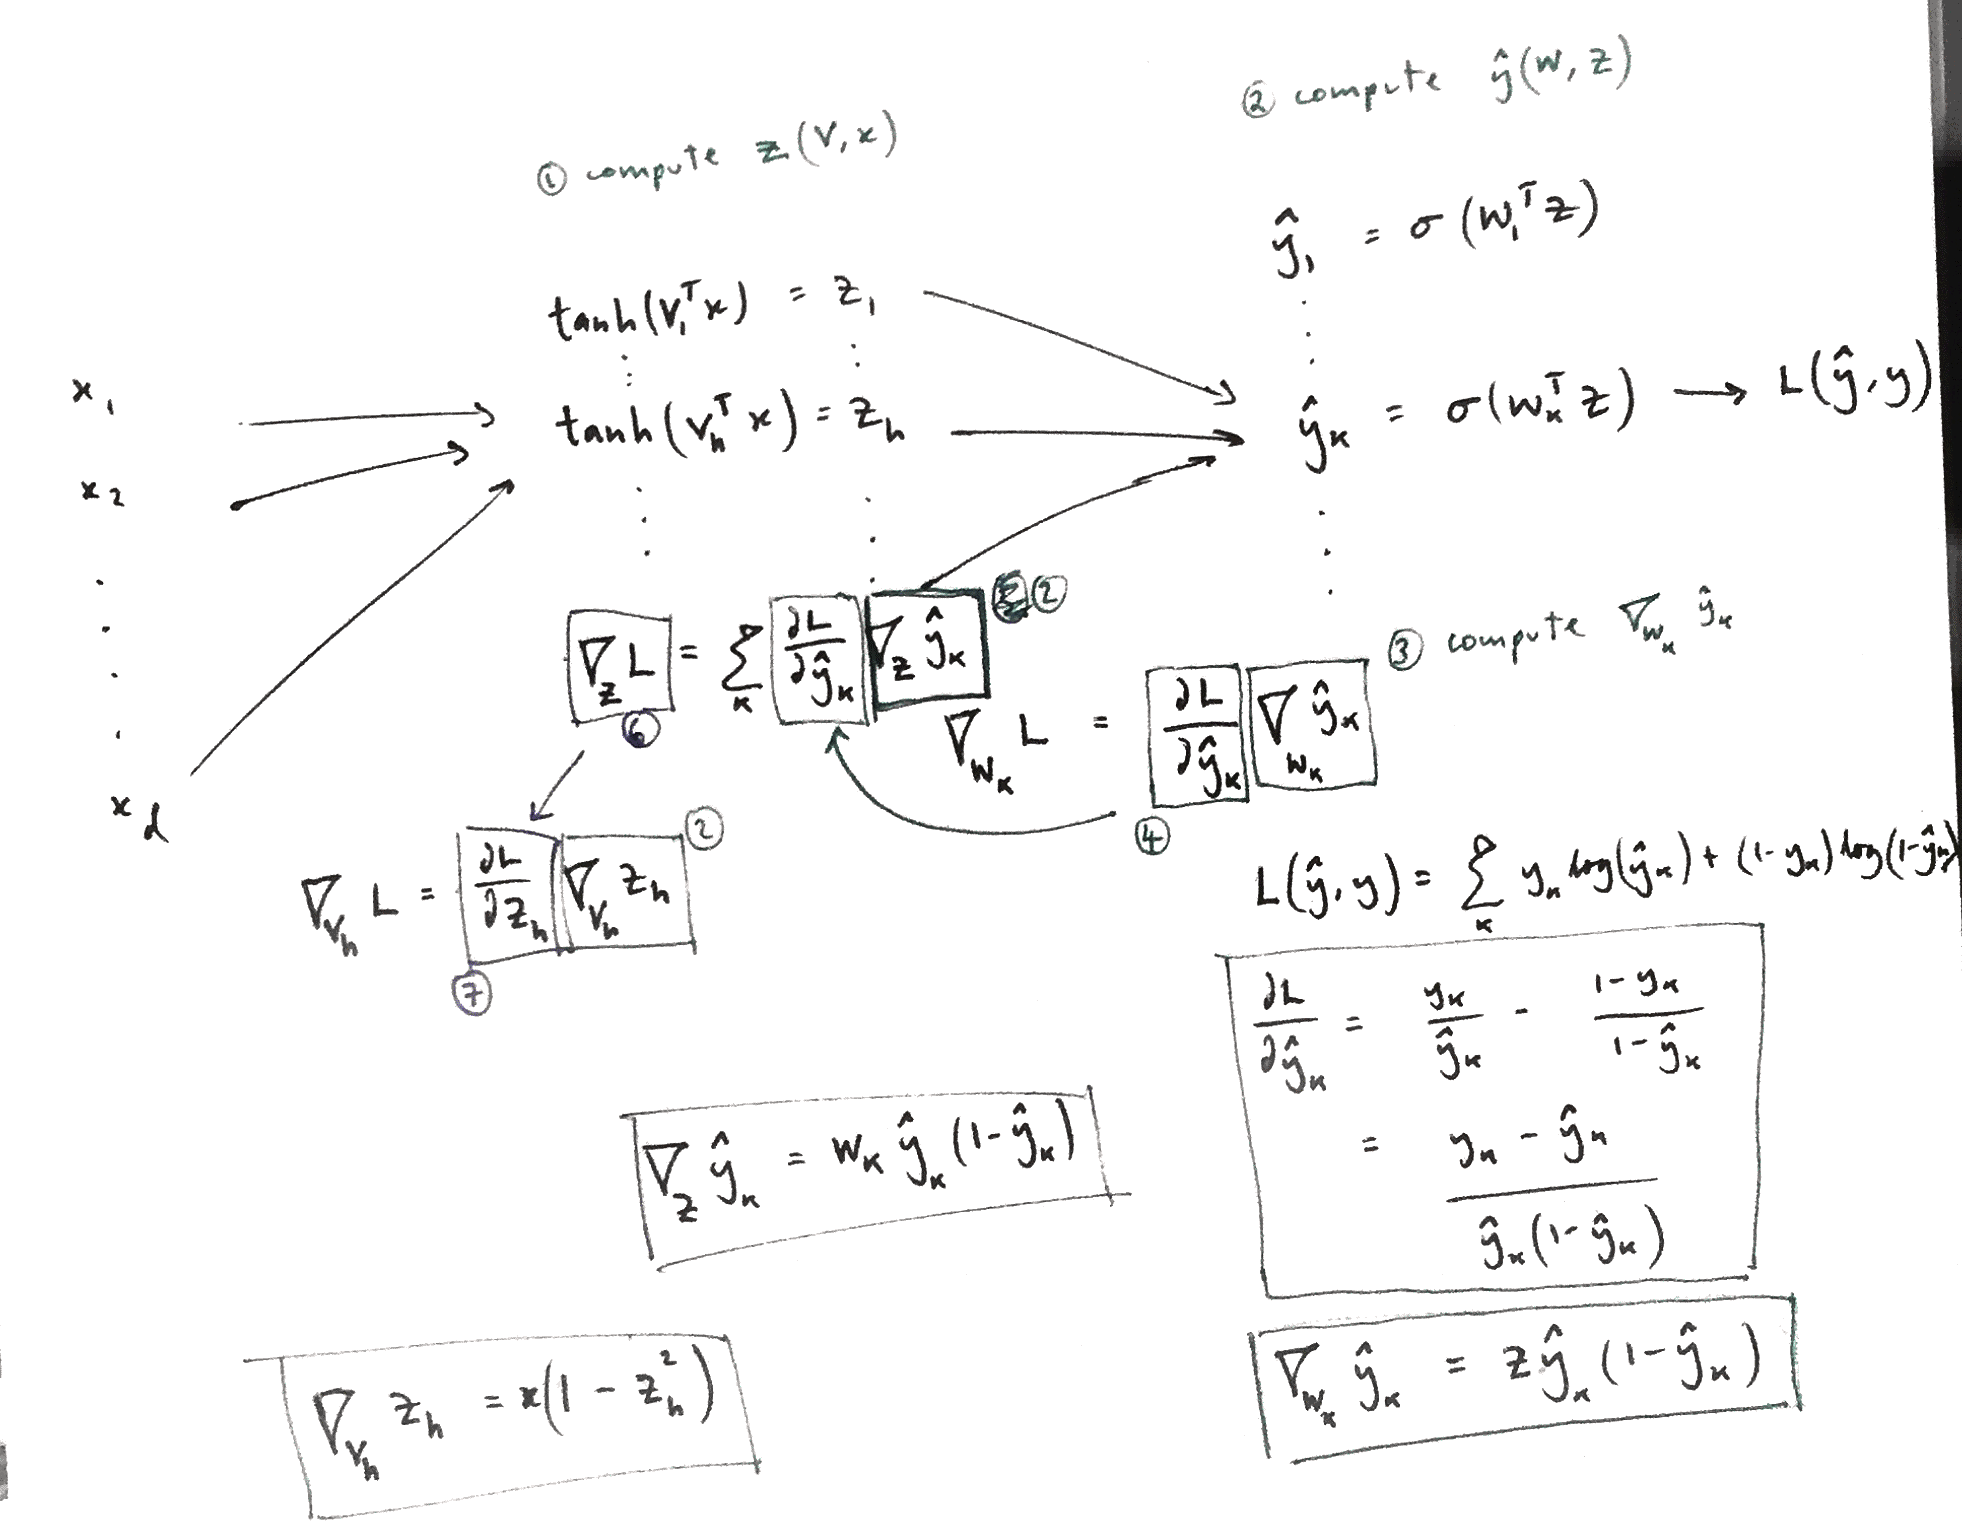
\includegraphics[width=500pt]{img/machine-learning-neural-net-backpropagation-1.png}

\subsection*{Trivial case}

\newcommand{\matrixiijj}[4]{\begin{bmatrix}#1 & #3\\#2 & #4\end{bmatrix}}
\newcommand{\matrixijj}[2]{\begin{bmatrix}#1 & #2\end{bmatrix}}

\subsubsection*{Forwards}

\begin{enumerate}
\item 1d input 0 with offset dimension: $x=\cvec{0}{1}$
\item $K=1$. Label $y = 1$
\item Initial $V = \matrixiijj{0}{0}{0}{0}$ (last row ignored)
\item $Vx = \matrixiijj{0}{0}{0}{0} \cvec{0}{1} = \cvec{0}{0}$ (last element ignored)
\item 1 hidden unit. $z \leftarrow \cvec{\tanh(0)}{1} = \cvec{0}{1}$
\item Initial $W = \matrixijj{0}{0}$
\item $Wz = \matrixijj{0}{0} \cvec{0}{1} = 0$
\item $\yhat = s(0) = 0.5$
\end{enumerate}

\subsubsection*{One iteration of backpropagation}

\begin{enumerate}
\item $\grad_{W_k} \yhat_k = \z \yhat_k(1 - \yhat_k) = \cvec{0}{0.25}$
\end{enumerate}

\begin{align*}
  \grad_{W_k} L &= \partiald{L}{\yhat_k} \grad_{W_k} \yhat_k \\
  \partiald{L}{\yhat_k} &= \frac{y_k - \yhat_k}{\yhat_k (1 - \yhat_k)} \\
  \grad_{W_k} \yhat_k &= z \yhat_k (1 - \yhat_k) \\
\end{align*}

\begin{align*}
  \grad_z L &= \sum_k \partiald{L}{\yhat_k} \grad_z \yhat_k \\
  \grad_z \yhat_k &= W_k \yhat_k (1 - \yhat_k) \\
\end{align*}

\begin{align*}
  \grad_{V_h} L &= \partiald{L}{z_h} \grad_{V_h} z_h \\
  \grad_{V_h} z_h &= x(1 - z_h^2)
\end{align*}




\section*{Classification}

A \textbf{decision boundary} is a curve separating the plane (sample space)
into two regions.

Some classifiers involve a \textbf{decision function} $f$, in which case
$f(\x) = 0$ describes the decision boundary.

A \textbf{linear classifier} uses a linear decision function
$f(x) = \w \cdot \x + \alpha$. This is scalar-valued: it's a plane over
the plane (sample space). Its intersection defines a linear decision boundary.

In $d$-dimensions the decision boundary is a hyperplane
($(d-1)$-dimensional). This still separates the sample space into two regions.

\textbf{Example:} $f(x) = \cvec{1}{1} \cdot \cvec{x_1}{x_2} + 4$
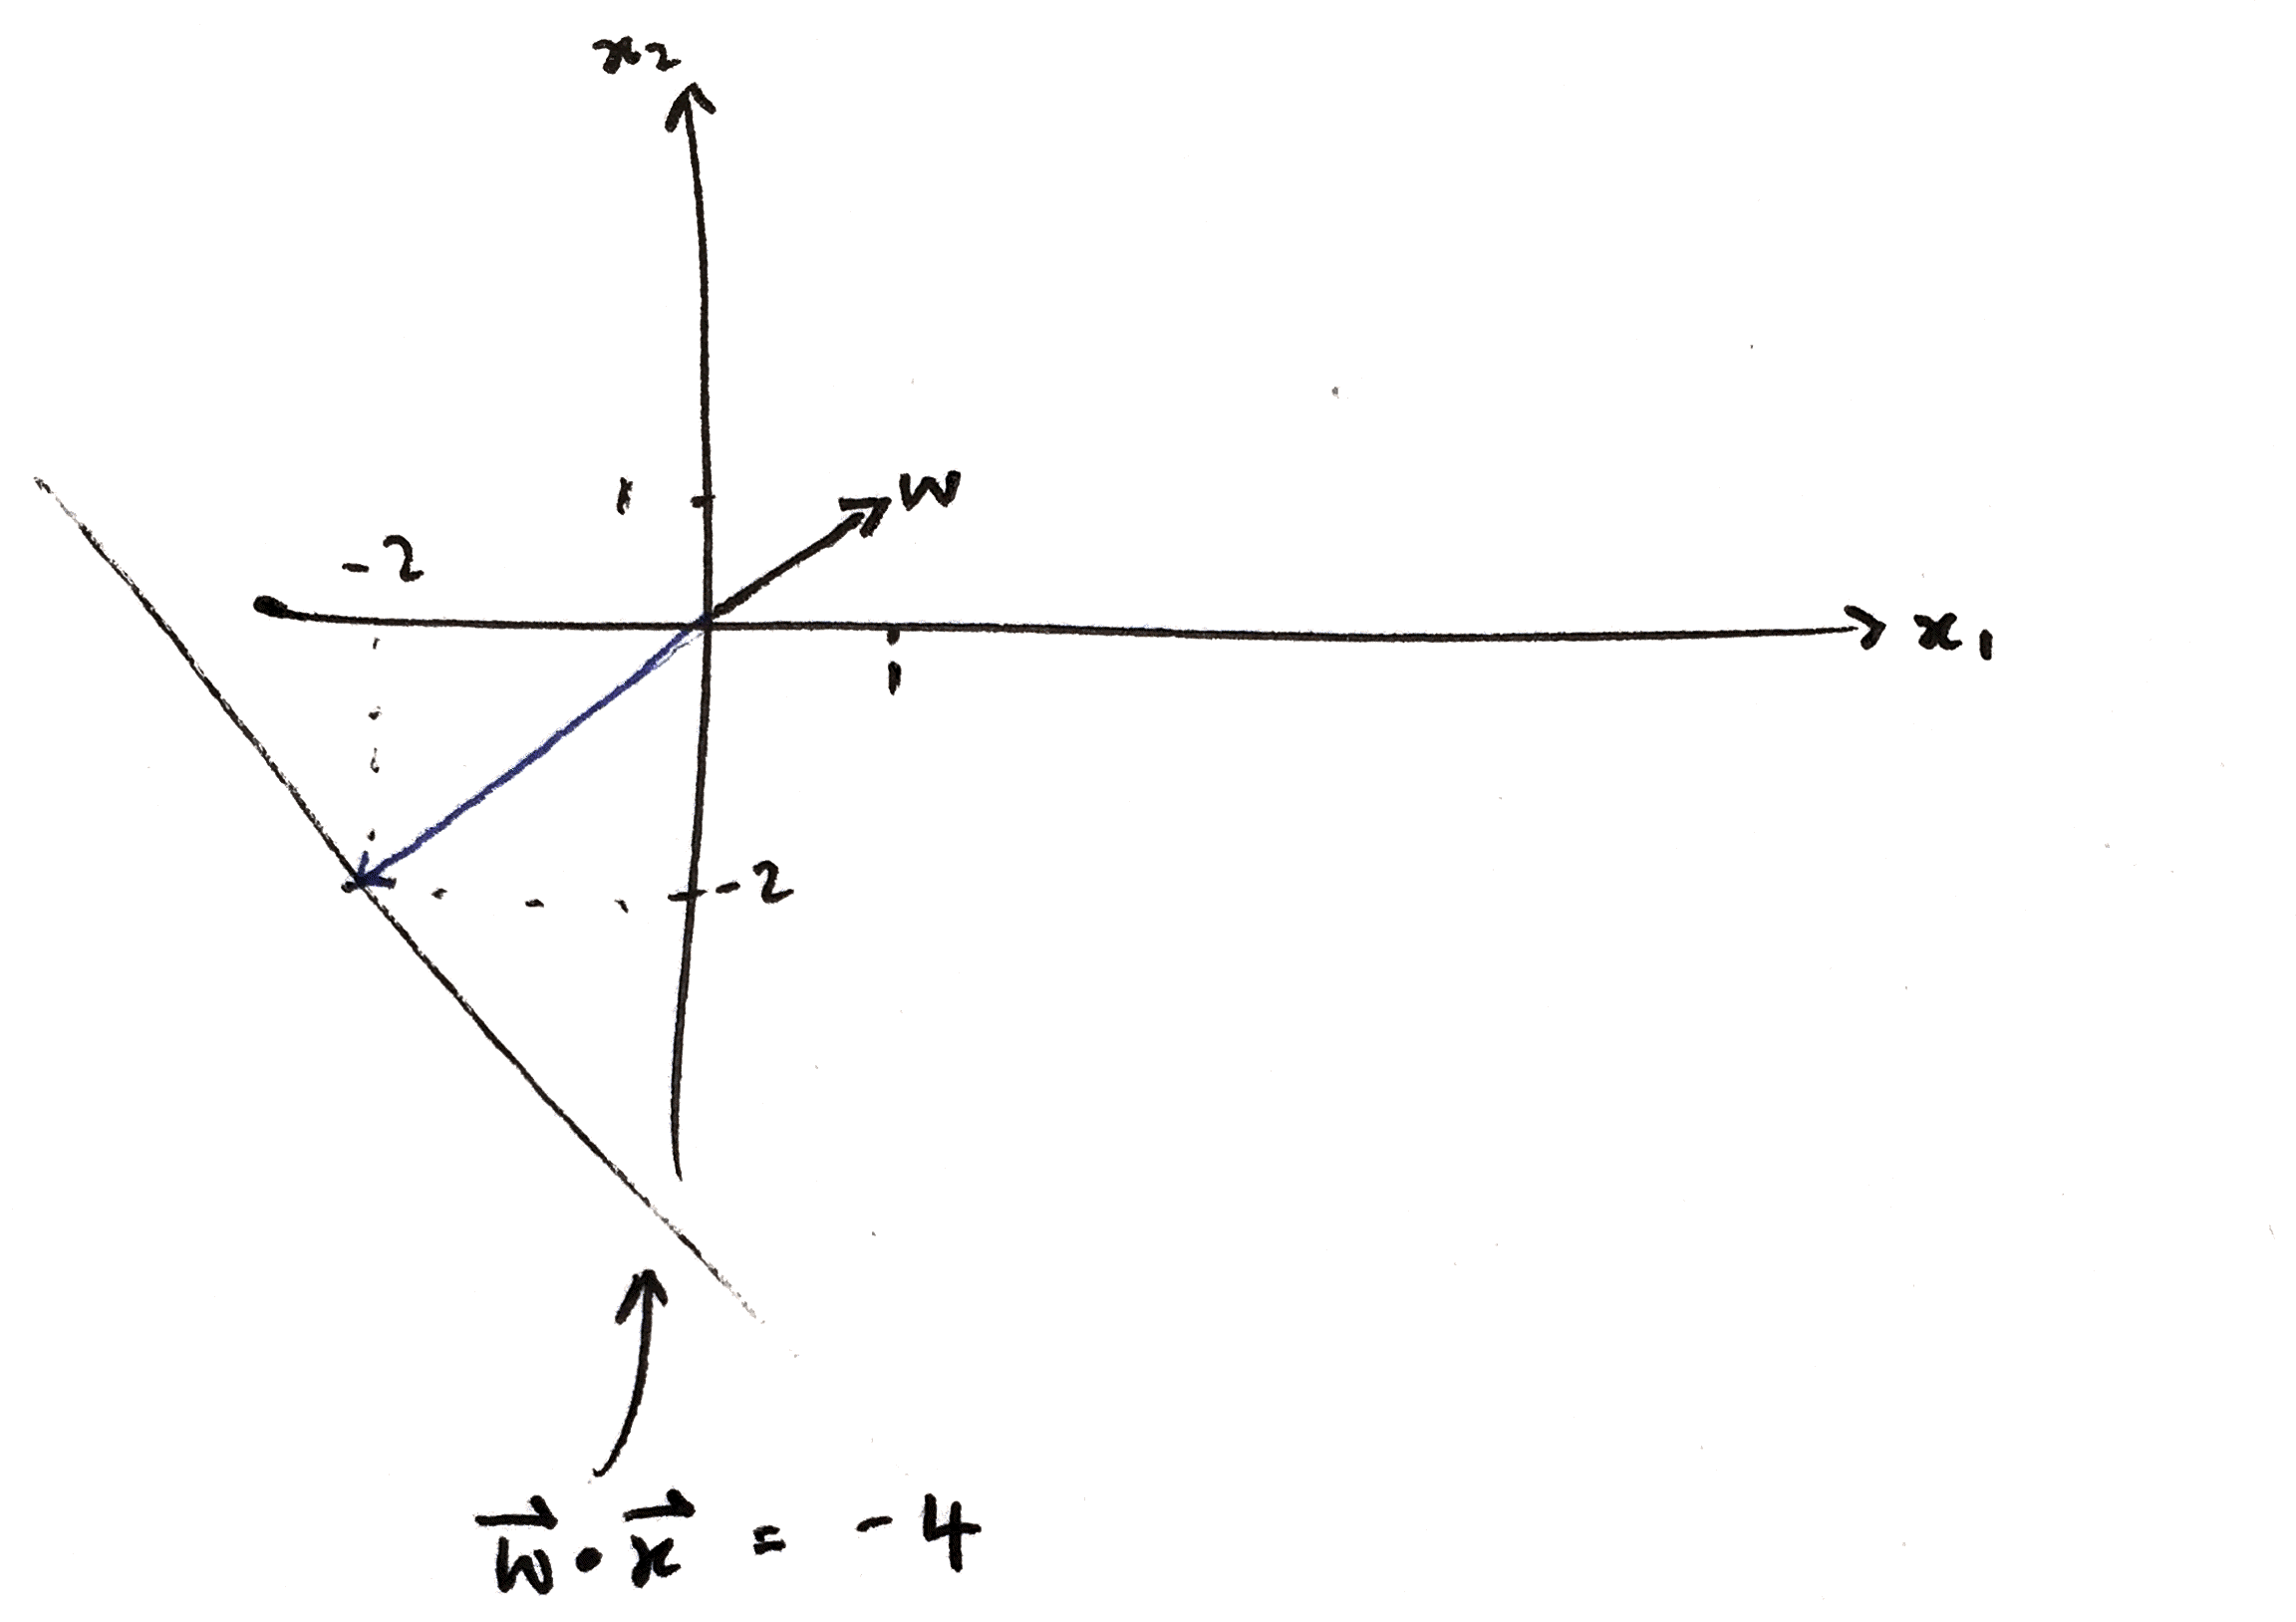
\includegraphics[width=200pt]{img/machine-learning-linear-decision-boundary.png}
\begin{itemize}
\item A plane sloping up at 45° in the north-east direction.
\item Each input feature has equal influence on the classification.
\item Decision boundary is line $x_1 + x_2 = -4$.
\item $\w$ is normal to the decision boundary since $\w \cdot (\x_1 - \x_2) = -4 - (-4) = 0$.
\item If one feature has a very high weight then $\w$ points close to that
  axis and the decision boundary is almost perpendicular to that axis (other
  features almost don't matter).
\end{itemize}

\textbf{Distance from the decision boundary to a point}: For some point $\x_i$,
the height of the decision function plane above $\x_i$ is
$\w \cdot \x_i + \alpha$. At the decision boundary, this height is
zero. Looking ``straight up'' the slope of the decision function, its gradient
is $\sqrt{w_1^2 + w_2^2} = |\w|$. So the distance of a point $\x_i$ from the
hyperplane is $\frac{\w \cdot \x_i + \alpha}{|\w|}$. If $\w$ is not a unit
vector, the problem can be rescaled so that it is, in which case the distance
is $\w \cdot \x_i + \alpha$.
\\
% \begin{mdframed}
%   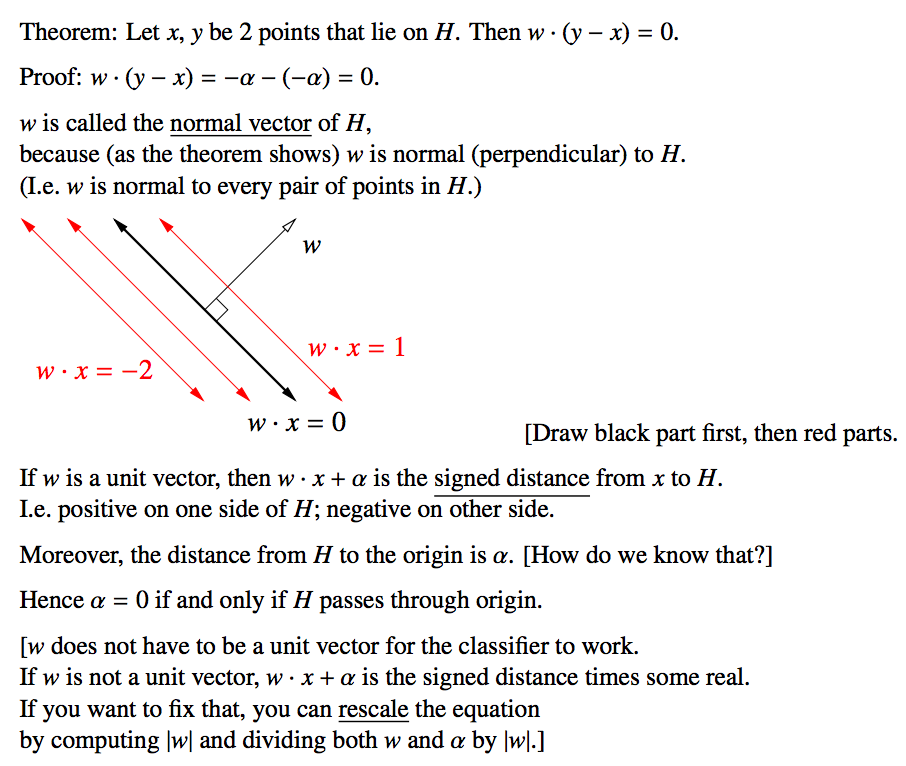
\includegraphics[width=300pt]{img/machine-learning-linear-decision-boundary-2.png}
% \end{mdframed}

\textbf{Examples of linear classifiers}:
\begin{itemize}
\item \textbf{Centroid method}:  Decision boundary perpendicular to and bisects line
  connecting means of labeled training points.
\item \textbf{Perceptron}:
\item \textbf{Maximum margin classifier}:
\item \textbf{LDA}:  Fit Gaussians to each class, same covariance across classes.
\end{itemize}

\subsection*{Perceptron}

Labels $y_i \in \{-1, 1\}$. Assume $\alpha=0$ for now (decision boundary through origin).

\textbf{Goal}: find line separating points (separating hyperplane). I.e. Find $\w$ such that
\begin{align*}
  \begin{cases}
    \x_i \cdot \w \leq 0, &y_i = -1 \\
    \x_i \cdot \w \geq 0, &y_i = +1.
  \end{cases}
\end{align*}
This is equivalent to the \textbf{constraint} $y_i\x_i \cdot \w \geq 0$.

\textbf{Cost function}: total distance $R(\w)$ of misclassified points from the
decision boundary.
\\
\begin{mdframed}
  \textbf{Optimization problem}: Find $\w$ that minimizes
  \begin{align*}
    R(w) = \sum_i L(\x_i \cdot \w, y_i) = \sum_{i \in V} -y_i\x_i \cdot \w,
  \end{align*}
  where $V$ are the misclassified points.
\end{mdframed}

Per-training point loss function
\begin{align*}
  L(\text{prediction}_i, y_i) = L(\x_i \cdot \w, y_i) =
  \begin{cases}
    0, &\text{correct}, y_i\x_i \cdot \w \geq 0\\
    -y_i\x_i \cdot \w, &\text{misclassified}
  \end{cases}
\end{align*}


\textbf{Gradient descent}: Find $w$ that minimizes $R(w)$.


\begin{align*}
  \nabla_w R = \cveccc{-\sum_i y_iX_{i1}}
                      {\vdots}
                      {-\sum_i y_iX_{id}}
\end{align*}
\begin{itemize}
\item On each iteration, compute the gradient; update $\w$ by taking a step
  downhill of size $\rho$: $\w \leftarrow \w + \rho \sum_{i \in V} y_i\x_i$.
\item A misclassified data point far out in dimension $j$ will cause the
  gradient to have a large component $-\sum_i y_iX_{ij}$ in that dimension.
\item $\w$ thus becomes more closely aligned with that axis and the decision
  boundary.
\item Decision boundary therefore becomes more perpendicular to that axis (axis
  becomes more ``important'').
\end{itemize}

\textbf{Stochastic gradient descent (Perceptron)}: on each iteration pick one misclassified
point and update $\w$ using gradient for that point:
$\w \leftarrow \w + \rho y_{i^*}\x_{i^*}$

\textbf{Allow decision boundaries that do not pass through origin}: add a
fictitious dimension so that sample points now lie on the plane $x_{d+1} = 1$
in $(d+1)$ dimensions. Run algorithm as above, just with the new
dimensionality.
\begin{align*}
  \w \cdot \x + \alpha &= 0 \\
  \cveccc{w_1}
         {w_2}
         {\alpha} \cdot \cveccc{x_1}{x_2}{1} &= 0.
\end{align*}

\subsection*{Optimization in weight space}

\begin{tabular}{l|l}
  $\x$-space    & $\w$-space \\
  \hline
  hyperplane & point $\w$ is normal vector to hyperplane \\
  point      & hyperplane whose normal vector is the $\x$ point (? don't understand this yet)
\end{tabular}

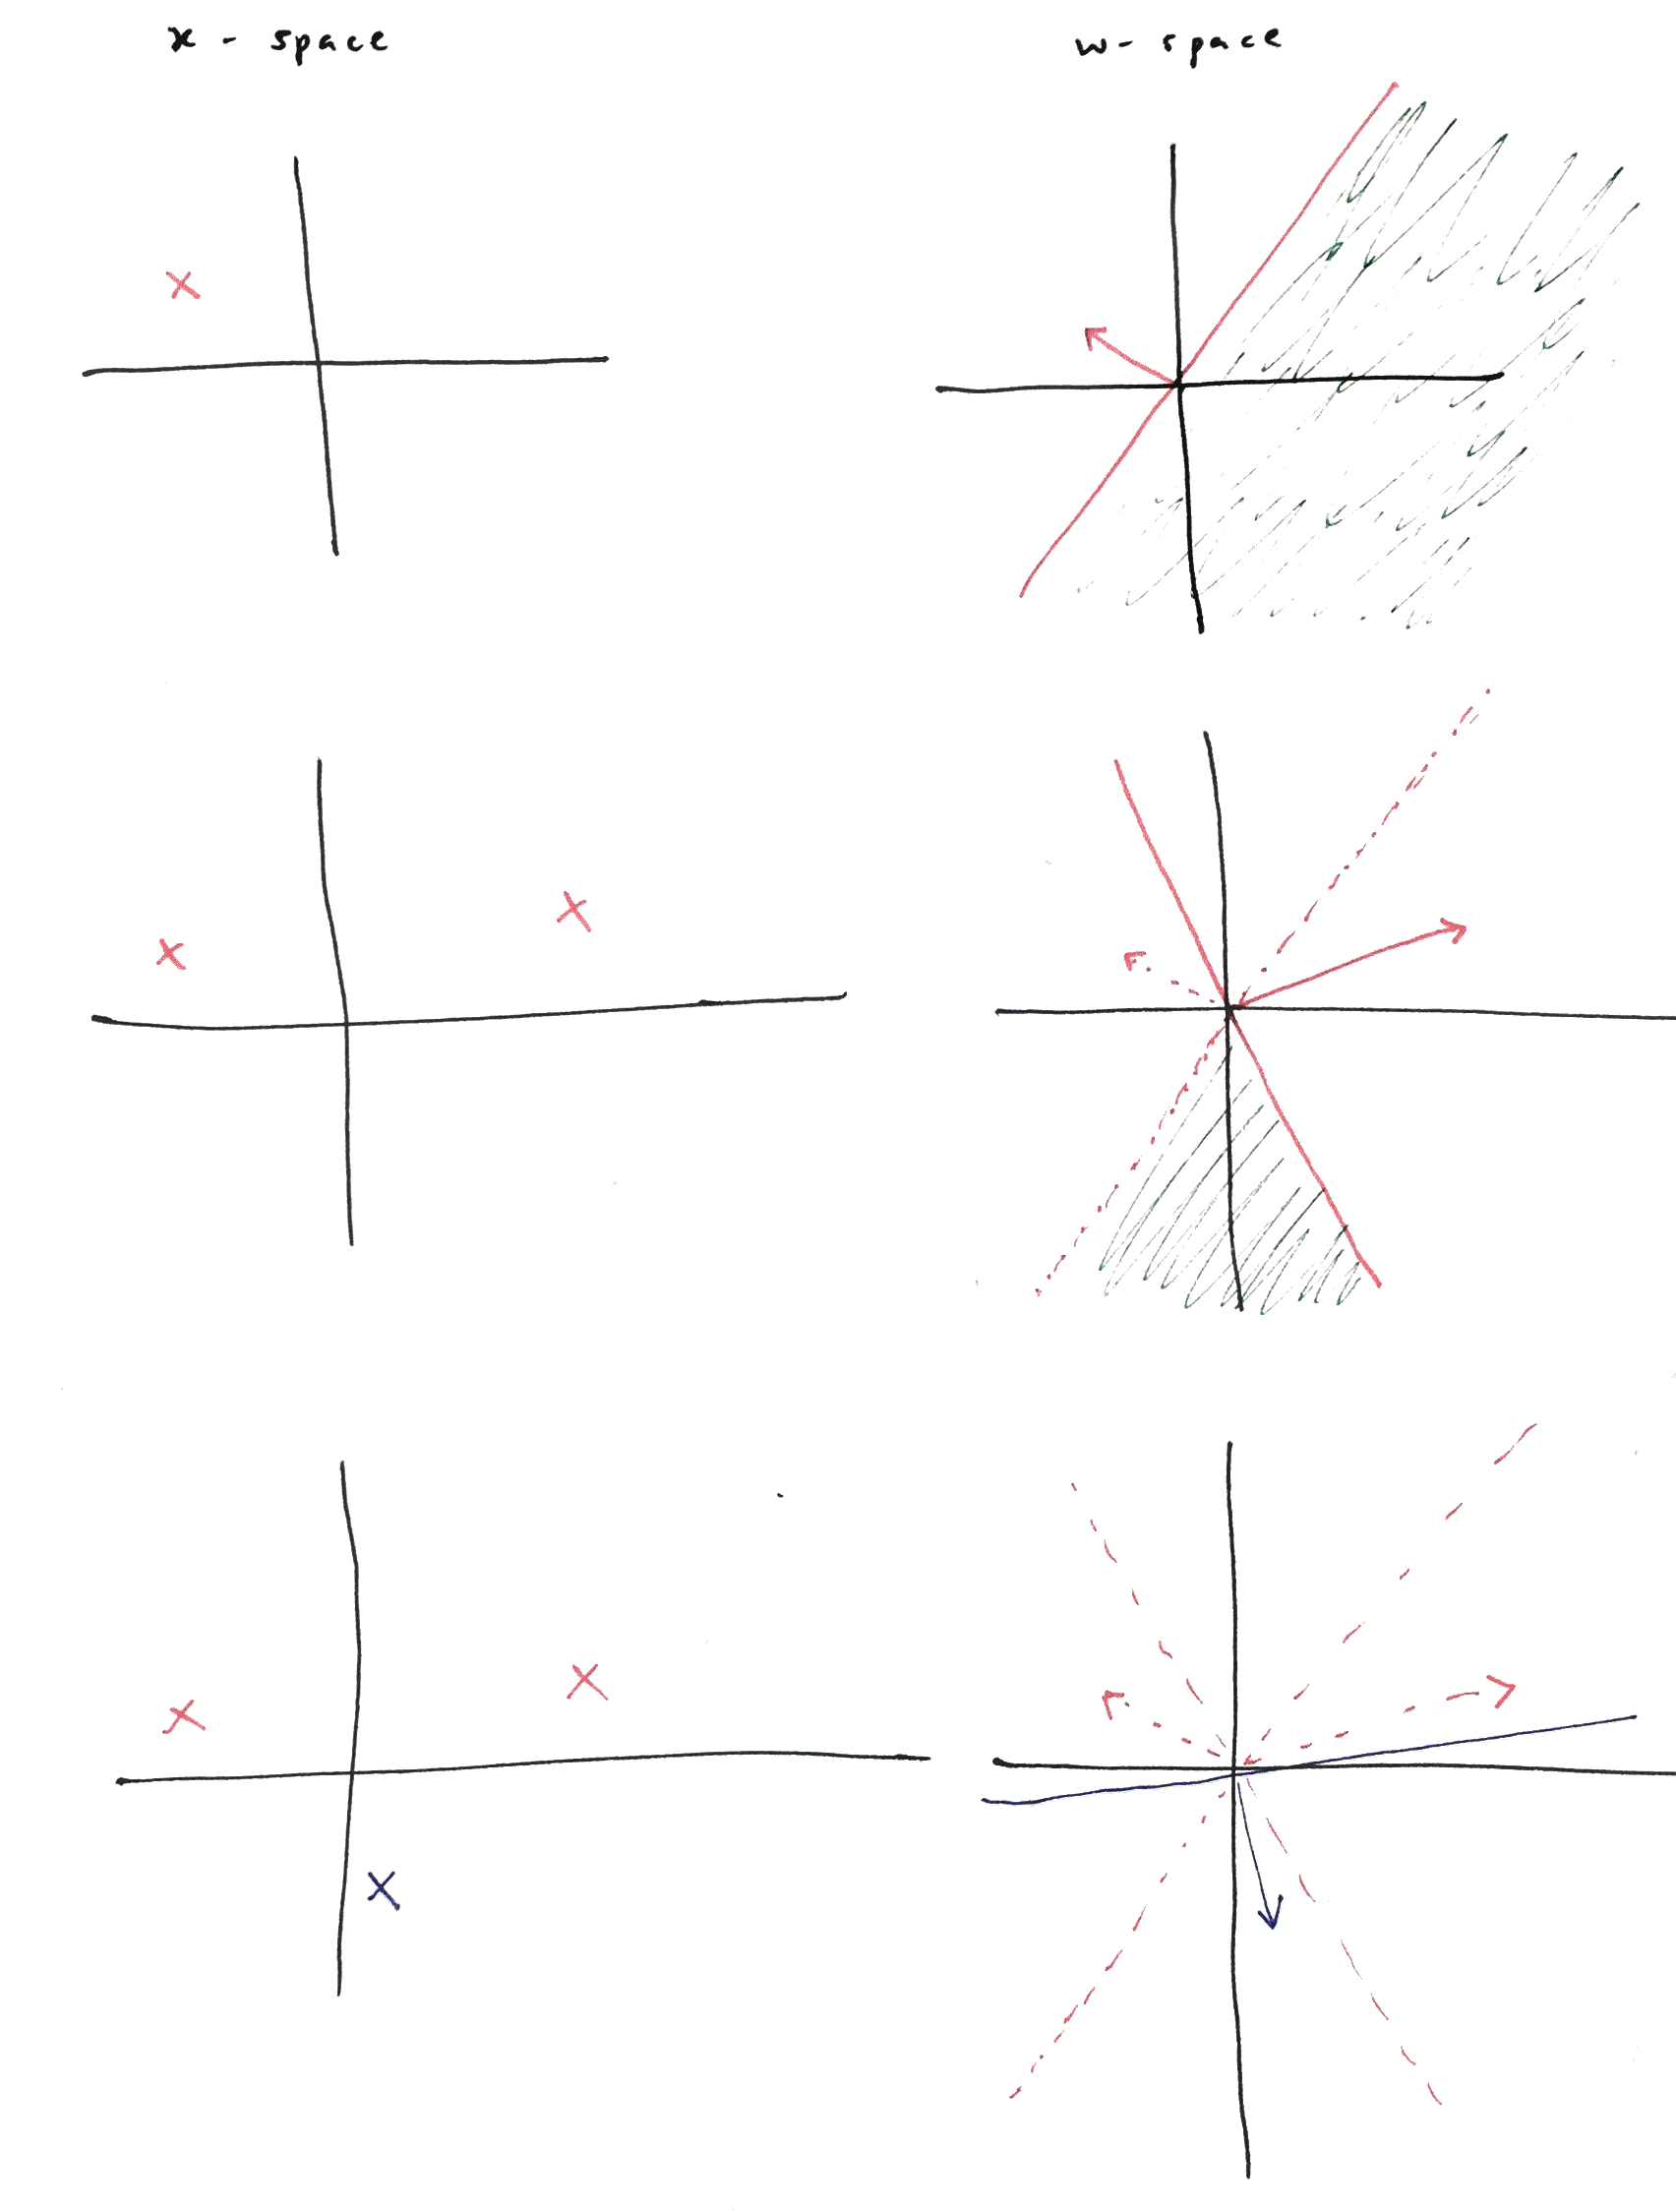
\includegraphics[width=200pt]{img/ml-perceptron-x-space-w-space.png}

\subsection*{Maximum margin classifiers}
\textbf{Margin} is distance from hyperplane to nearest sample point.

Previously, in the perceptron, we used the constraint
$$y_i \x_i \cdot \w \geq 0.$$
Now, we demand that there is a non-zero margin between the decision boundary
and the points:
$$y_i (\x_i \cdot \w + \alpha) \geq 1,$$
The 1 on the RHS is arbitrary; I think $\w$ and $\alpha$ will adapt to make it
true for any positive value, so the point is that we're demanding a strictly
non-zero margin.
\\
\begin{mdframed}
  \textbf{Optimization problem (quadratic program)}:\\
    Find $\w, \alpha$ that minimize $|\w|^2$ such that
    $y_i(\x_i \cdot \w + \alpha) \geq 1$ for all points $i$.
\end{mdframed}

\subsection*{Soft margin SVMs
\footnote{\url{https://people.eecs.berkeley.edu/~jrs/189/lec/04.pdf}}
\footnote{ \url{https://www.youtube.com/watch?v=HOZ6ZpPA_Ks}}
}

\begin{itemize}
\item Still quadratic program but allow points to violate margin via
  \textbf{slack variables} $\xi_i \geq 0$:
\item Constraint is $y_i(\x_i \cdot \w + \alpha) \geq 1 - \xi_i$
\item Find non-linear decision boundaries by introducing new features
  comprising non-linear functions of base features (``lift points into
  higher-dimensional space'').
\end{itemize}

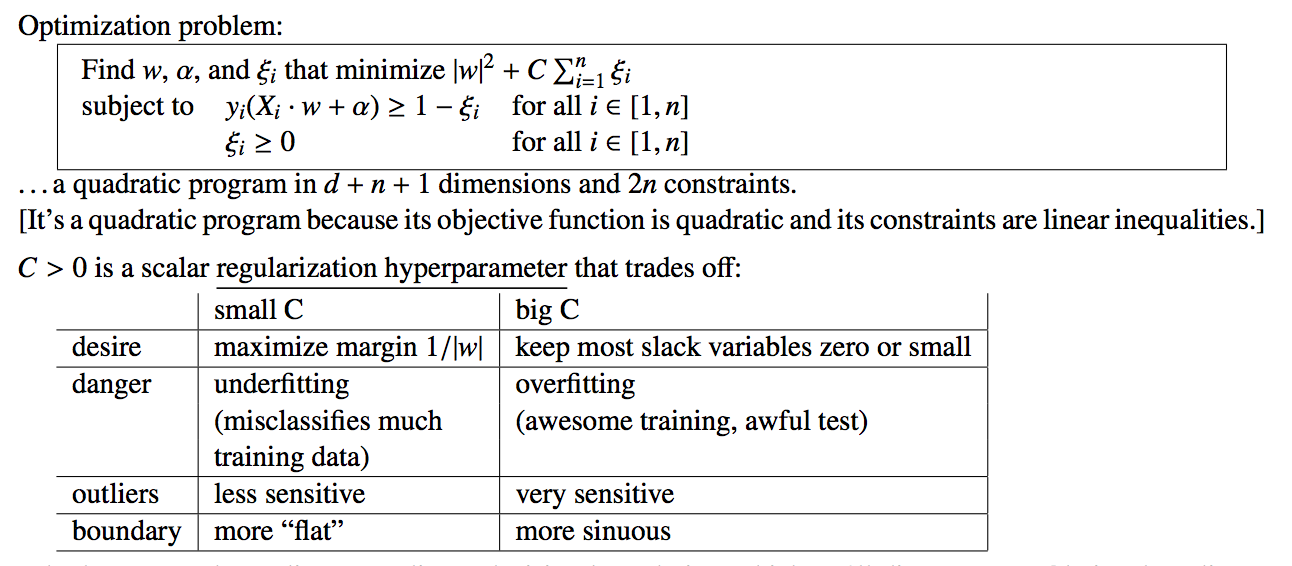
\includegraphics[width=300pt]{img/machine-learning-svm-1.png}
% 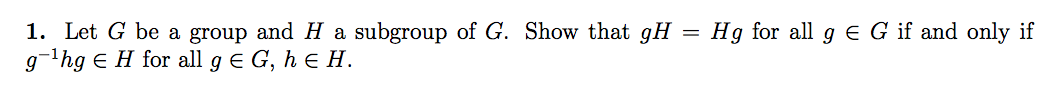
\includegraphics[width=300pt]{img/ml-svm-parabolic-lifting.png}



% \section*{5 Machine Learning Abstractions and Numerical Optimization}
% \url{https://people.eecs.berkeley.edu/~jrs/189/lec/05.pdf}\\
% \url{https://www.youtube.com/watch?v=DeIAXPUfCbQ}

\newpage
\section*{Decision Theory
  \footnote{\url{https://people.eecs.berkeley.edu/~jrs/189/lec/06.pdf}}
  \footnote{\url{https://www.youtube.com/watch?v=aXkenQ01qYI}}
}

Suppose there are two possible \textbf{classes}: $\{C, D\}$

\textbf{Decision rule}: $r(\x): \R^d \to \{C, D\}$

\textbf{Loss function}: E.g. 0-1 loss:
\begin{align*}
  L(y_i \to \hat y_i) =
  \begin{cases}
    0, & \hat y_i = y_i ~~~~~~~~~~~~~~~~~~~~\text{(correct classification)}\\
    1, & \otherwise
  \end{cases}
\end{align*}

\textbf{Risk}: Functional $R(r)$: expected loss for rule $r$, over $\p(X, Y)$.
\footnote{
\begin{align*}
  R(r) = &\pi(Y=-1)\E_\X L(-1 \to r(X)) + \\
         &\pi(Y=+1)\E_\X L(+1 \to r(X))~~~~~~~~~~~~~~~~~~~~~~~\text{over $\p(Y)\p(X|Y)$}
\end{align*}
\begin{align*}
  = \sum_X \p(X)\big(&\pi(Y=-1)L(-1 \to r(X)) + \\
                     &\pi(Y=+1)L(+1 \to r(X))\big)~~~~~\text{over $\p(X)\p(Y|X)$}
\end{align*}
}

So what rule function $r$ minimizes the functional $R$?

\textbf{Bayes decision rule}: Assign $\x$ to class $C$ if

\begin{center}
(C posterior at $\x$) $\times$ (penalty for misclassifing a true C)
\end{center}

is largest for class $C$. I.e. if
\begin{align*}
  \p(C|\x)L(D|C) > \p(D|\x)L(C|D).
\end{align*}

With 0-1 loss, this is: ``assign to class with highest posterior''.

With 0-1 loss and two classes, it's: ``assign to class with posterior $> 0.5$''.

\textbf{Empirical risk}: Discriminative methods (e.g. logistic regression) lack
any model for $X$. How can we estimate expected loss over $p(X,Y)$? Take the
observed sample points as defining a discrete, uniform distribution, in which
case
\begin{align*}
  \hat R(r) = \frac{1}{n}\sum L(r(x_i), y_i).
\end{align*}
This provides a justification for minimizing the sum/mean of per-sample loss.

\newpage
\section*{Statistical justifications}

Regression: want to estimate a function $f$ such that
$y_i = f(x_i) + \epsilon$, where $\epsilon$ has unknown distribution but mean
0. Ideal would be to estimate $f$ with $h(x_i) = \E(Y|x_i)$ since this is equal
to $f(x_i)$.

Likelihood justification for linear regression cost function.

Logistic Regression from Maximum Likelihood

\section*{Bias-Variance Decomposition}

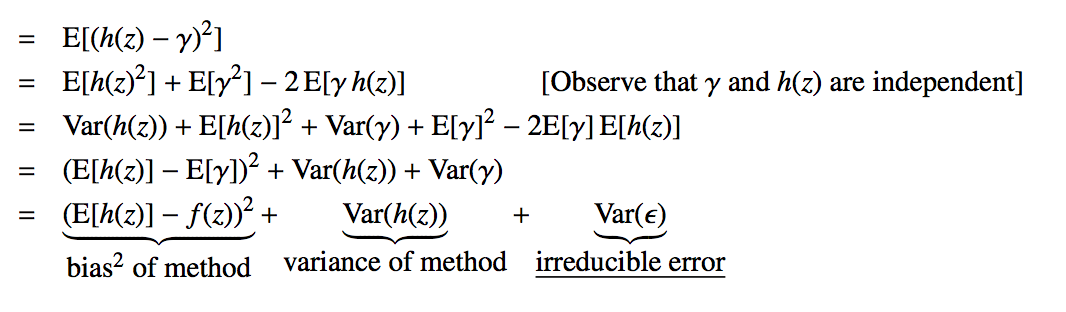
\includegraphics[width=300pt]{img/machine-learning-bias-variance-decomp-1.png}





\newpage
\section*{Gaussian discriminant analysis
  \footnote{\url{https://people.eecs.berkeley.edu/~jrs/189/lec/07.pdf}}
  \footnote{\url{https://www.youtube.com/watch?v=4CefboCXxZs}}
}

\textbf{Anisotropic}:
\begin{align*}
  \p(\x) = \frac{1}{(2\pi)^{d/2}|\Sigma|^{1/2}} \exp\(-\frac{1}{2}(\x - \mu)^\T\Sigma^\1(\x - \mu)\)
\end{align*}

\textbf{Isotropic}:
\begin{align*}
  \p(\x) = \frac{1}{(2\pi)^{d/2}\sigma^d} \exp\(-\frac{|\x - \mu|^2}{2\sigma^2}\)
\end{align*}

\newcommand{\class}{\text{class~}}

\subsection*{Isotropic Gaussians}

Multivariate data $\x$ but features uncorrelated and all features same variance.

\subsubsection*{QDA}
Fit separate Gaussians to the training data in each class. The likelihood is
\begin{align*}
  \p(\x|\class C) = \frac{1}{(2\pi)^{d/2}\sigma_C^d}\exp\(-\frac{|\x - \mu_C|^2}{\sigma_C^2}\)
\end{align*}

and we compare the value of $\p(\x|\class C) \cdot \pi_C \cdot L(D|C)$.

The decision boundaries are where the posterior $\times$ loss are equal. It's
easier to compare the log of this:
\begin{align*}
  Q_C(\x) = - \frac{|\x - \mu_C|^2}{\sigma_C^2} - d\log \sigma_C + \log \pi_C + \log L(D|C)
\end{align*}

\begin{comment}
  So the decision boundary is at $\x$ satisfying
  \begin{align*}
    Q_C(\x) - Q_D(\x) &= 0 \\
    \frac{|\x - \mu_D|^2}{\sigma_D^2} - \frac{|\x - \mu_C|^2}{\sigma_C^2} +
    d\log \frac{\sigma_D}{\sigma_C} +
    \log \frac{\pi(C)}{\pi(D)} +
    \log \frac{L(D|C)}{L(C|D)}
     &= 0 \\
  \end{align*}
\end{comment}

The posterior probability of class $C$ at point $\x$ is\footnote{This is
  assuming 0-1 loss, so the loss doesn't affect $Q_C(\x)$}
\begin{align*}
  \p(C|\x)
  = \frac{\pi_C\p(\x|C)}{\pi_C\p(\x|C) + \pi_D\p(\x|D)}
  = \frac{1}{1 + e^{-(Q_C(\x) - Q_D(\x))}},
\end{align*}
so logistic in the quadratic expression $Q_C(\x) - Q_D(\x)$.

\subsubsection*{LDA}
Estimate separate class means but same variance for all classes. So now
\begin{align*}
  Q_C(\x) - Q_D(\x)
  &= \frac{|\x - \mu_D|^2 - |\x - \mu_C|^2}{\sigma^2} + \log \frac{\pi_C}{\pi_D} + \log \frac{L(D|C)}{L(C|D)} \\
  &= \frac{(\x - \mu_D)\cdot(\x - \mu_D) - (\x - \mu_C)\cdot(\x - \mu_C)}{\sigma^2} + \log \frac{\pi_C}{\pi_D} + \log \frac{L(D|C)}{L(C|D)} \\
% &= \frac{ 2(\x\cdot\mu_C - \x\cdot\mu_D) + |\mu_D|^2 - |\mu_C|^2}{\sigma^2} + \log \frac{\pi_C}{\pi_D} + \log \frac{L(D|C)}{L(C|D)} \\
  &= \x\cdot\frac{2(\mu_C - \mu_D)}{\sigma^2} + \(\frac{|\mu_D|^2 - |\mu_C|^2}{\sigma^2} + \log \frac{\pi_C}{\pi_D} + \log \frac{L(D|C)}{L(C|D)}\) \\
  &= \x\cdot\w + \alpha
\end{align*}
This means that the decision boundary is linear, and (with 0-1 loss) the
posterior is a logistic function which is constant parallel to the decision
boundary.

\section*{Symmetric matrices, quadratic forms and eigenvectors
  \footnote{\url{https://people.eecs.berkeley.edu/~jrs/189/lec/08.pdf}}
}

\textbf{Spectral theorem}: A symmetric matrix has $n$ \textbf{orthogonal}
eigenvectors\footnote{There may be more than $n$ (infinite) eigenvectors, but
  $n$ orthogonal.}\footnote{Non-symmetric matrices have non-orthogonal eigenvectors in
  general.}


To understand a symmetric matrix $\A$, consider its \textbf{quadratic form}
$|\A\x|^2 = \x^\T \A^2\x$ (right). Compare this to the graph of $|\z|^2$
(left). The graphs are related by the following changes of coordinates:

$\z \gets \A\x$ changes the elliptical contours into circles; scale by eigenvalues of $\A$.

$\A^\1 \z \to \x$ changes circles into ellipses; scale by reciprocal of eigenvalues.

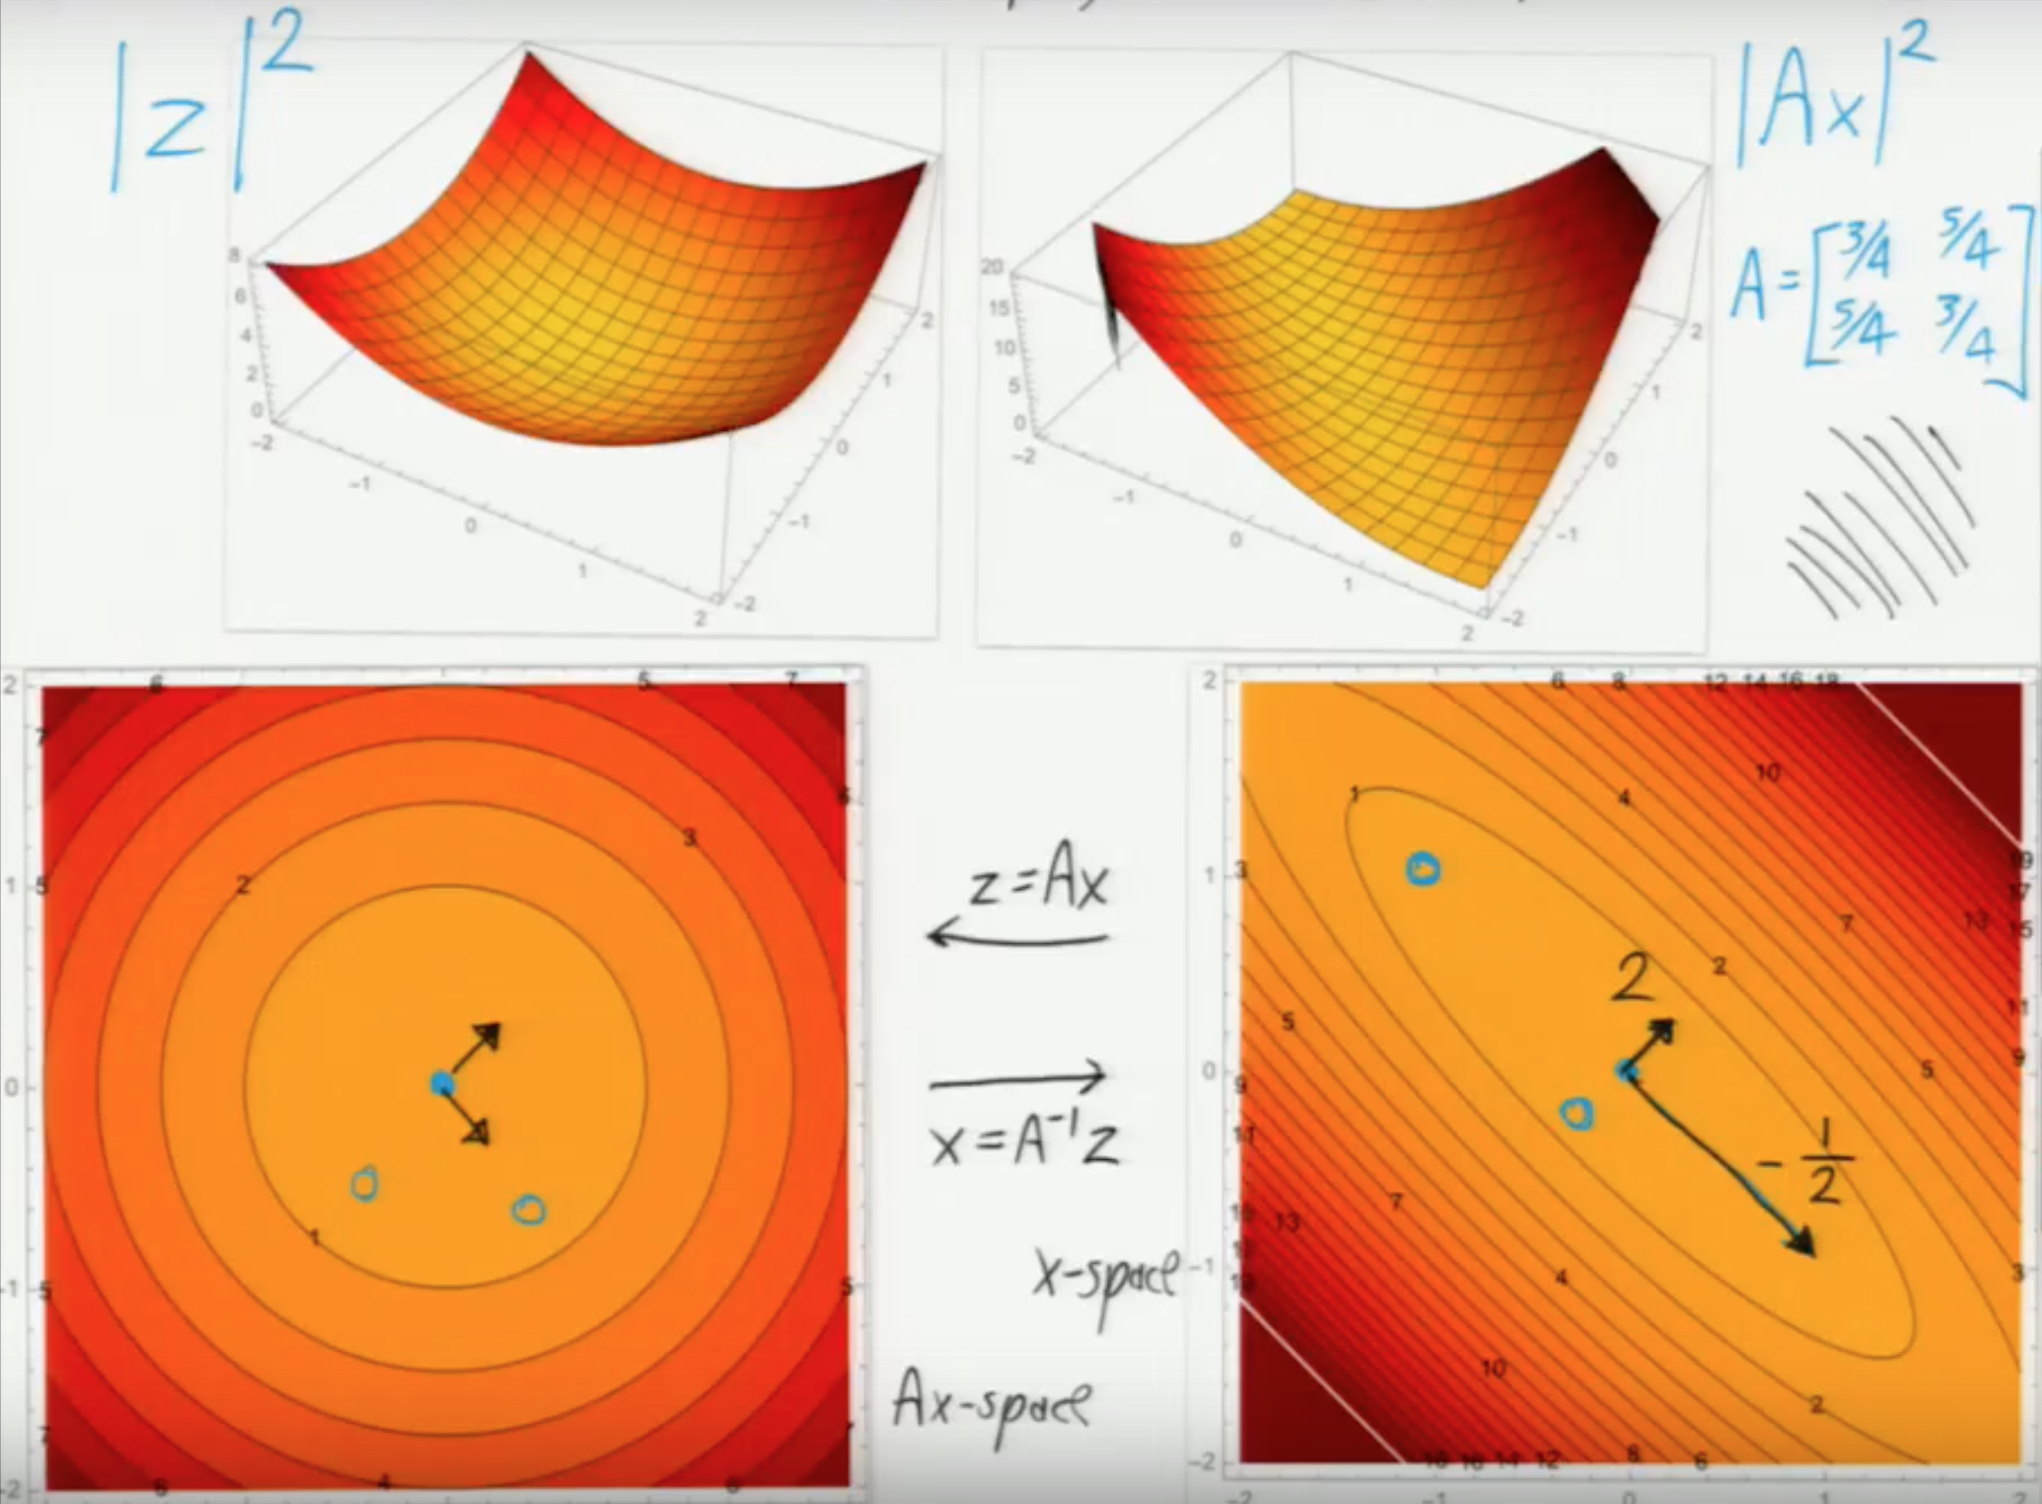
\includegraphics[width=300pt]{img/machine-learning-quadratic-form-eigenvectors.png}

$|\A\x|^2 = 1$ is the equation of an ellipsoid. Its axes are $v_1,\ldots,v_n$
and its radii are $\frac{1}{\lambda_1},\ldots,\frac{1}{\lambda_n},$

Bigger eigenvalue $\iff$ steeper hill.

Alternate interpretation: the ellipsoids are spheres in a space with a
different distance metric. The distance metric (metric tensor) is $\mat M=\A^2$:
\begin{align*}
  d(\x,\x') = |\A\x| - |\A\x'| = \sqrt{(\x - \x')\A^2(\x - \x')}
\end{align*}


\begin{minipage}{\textwidth}
These are diagrams of $\x^\T\A\x$ (not $\x^\T\A^2\x$ since $\A^2$ has no negative eigenvalues):

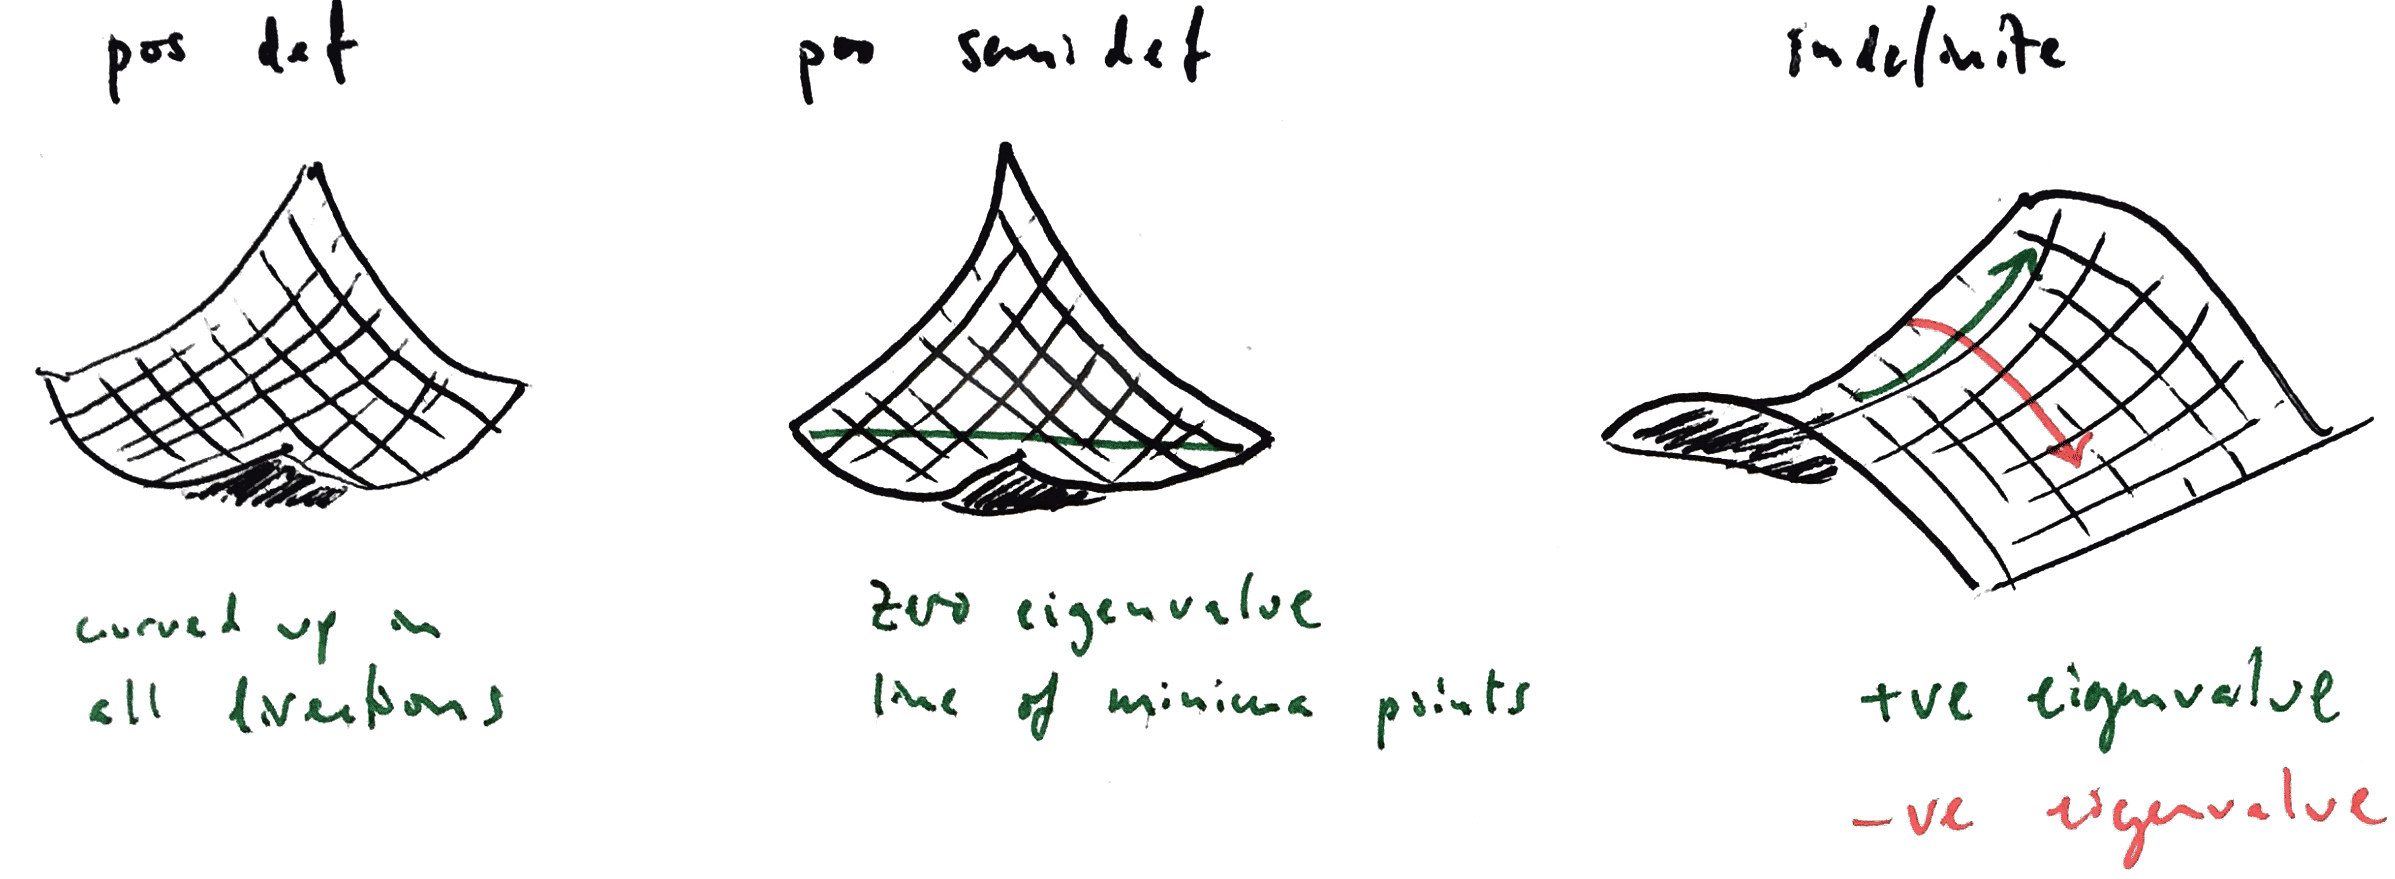
\includegraphics[width=300pt]{img/machine-learning-quadratic-form-eigenvectors-2.png}

\begin{tabular}{ l | l | l }
  \textbf{positive definite}     & eigenvalues $> 0$    & $\x^\T\A\x > 0 ~~~~~~ \forall \x \neq \0$ \\
  \textbf{positive semidefinite} & eigenvalues $\geq 0$ & $\x^\T\A\x >= 0 ~~~~ \forall \x$ \\
  \textbf{indefinite}            & some positive and some negative eigenvalues & \\
  \textbf{singular}              & some zero eigenvalue \\
\end{tabular}
\end{minipage}

Let $\Lambda$ be a diagonal matrix containing the eigenvalues and $\V$ contain
normalized eigenvectors:
\begin{align*}
V = \begin{bmatrix}
\mid & \mid & & \mid \\
\v_1 & \v_2 & \cdots & \v_n\\
\mid & \mid & & \mid \\
\end{bmatrix}
\end{align*}

Note that for an \textbf{orthonormal} matrix like this:
\begin{enumerate}
\item It rotates / reflects the input vectors, without changing their length.
\item  $\V^T\V = \I$, therefore $\V^\1 = \V^\T$.
\end{enumerate}


By the definition of eigenvector we have
\begin{align*}
  \A\V = \V\Lambda
\end{align*}
and therefore the \textbf{eigendecomposition} of $\A$
\begin{align*}
  \A = \V\Lambda\V^\T.
\end{align*}

So we can perform $\A\x$ as $\V\Lambda\V^\T\x$, and $\A^k\x$ as
$\V\Lambda^k\V^\T\x$:

\begin{enumerate}
\item $\V^\T = \V^\1$ rotates the input vector into axis-aligned coordinates.
\item $\Lambda$ scales along different axes.
\item $\V$ returns to the original coordinates.
\end{enumerate}

$\Lambda$ is said to be the diagonalized version of $\A$.
\section*{9 The Anisotropic Multivariate Normal Distribution, QDA, and LDA}

\newpage
\section*{Regression}
\subsection*{Linear Least Squares Regression}
Use fictitious dimension trick, so that $\w$ includes the offset term $\alpha$
and $\X$ is $(n \times (d + 1))$.
\\
\begin{mdframed}
Find $\w$ that minimizes cost function $J(w)$: sum of squared difference between
linear predictor and observed training point.
\begin{align*}
  J(w) = |\X \w - \y|^2 = \sum_i (\x_i^\T\w - y_i)^2
\end{align*}
\end{mdframed}

Solve by differentiating and finding the critical point:
\begin{align*}
  |\X \w - \y|^2          &= \w^\T\X^\T\X\w - 2\y^\T\X\w + \y^\T\y \\
  \grad_\w |\X \w - \y|^2 &= 2 \X^\T\X\w - 2\X^\T\y \\
  \w^*                    &= (\X^\T\X)^{-1}\X^\T\y =: \X^+\y
\end{align*}
\begin{mdframed}
For a new sample point $\x$, the prediction is $\hat y = \x \cdot \w^*$.
\end{mdframed}

\subsubsection*{Related concepts}
\begin{itemize}
\item \textbf{normal equations}: linear system of $d$ equations in unknown $\w$ resulting from
  setting the gradient equal to zero: $\X^\T\X\w - \X^\T\y = \vec 0$
\item \textbf{pseudoinverse}: The matrix $\X^+ = (\X^\T\X)^{-1}\X^\T$ maps $\y$
  to $\w^*$. In general there's no $\w$ that solves $\X\w = \y$, but
  $\w^* = \X^+\y$ makes the LHS as close as possible to $\y$. So it behaves as
  a ``left inverse'' of $\X$, since $\X^+\X = \I$ and left-multiplying by $\X^+$
  gives the ``solution'' to $\X\w = \y$.
\item \textbf{projection matrix} or \textbf{hat matrix}: Still focusing on the
  training phase, the predictions are $\hat \y = \X\w^* = \X\X^+\y$. So
  $\X\X^+$ puts that hat on $\y$, or projects $\y$ onto the hyperplane, in the
  viewpoint described below.
\end{itemize}

\subsubsection*{Projection interpretation}
Usually we think of $n$ points in $\R^d$. But instead, consider a separate
column of the data for each feature: these are $d$ points in $\R^n$. The
observed training data $\y$ is also a point in $\R^n$, and so is the prediction
$\hat \y = \X\w$.

As we vary $\w$, the prediction $\X\w$ describes a hyperplane spanned by the
columns of $\X$.

We want to find the $\w^*$ corresponding to the closest point on the hyperplane
to $\y$. So $X\w^* - \y$ must be orthogonal to the hyperplane:
\begin{align*}
  \X^\T \cdot (\X\w^* - \y) = \vec 0.
\end{align*}
Which are the normal equations (linear system of $d$ equations), derived
differently.

\subsubsection*{Weighted linear regression}
Sample point $i$ has weight $b_i$. Diagonal $n \by n$ matrix $\mat B$ contains weights.
\begin{align*}
  J(\w) &= \sum_i b_i (\x_i^\T\w - y_i)^2 \\
        & = (\X\w - \y)^\T \B (\X\w - \y) \\
        &= \w^\T\X^\T \B \X\w - 2\y^\T \B \X\w + \y^\T\y
\end{align*}
Gradient
\begin{align*}
  \grad_\w J(\w) = 2\X^\T \B \X\w - 2\X^\T\B\y
\end{align*}
Solution
\begin{align*}
  \w^* = \(\X^\T \B \X\)^{-1}\X^\T\B\y
\end{align*}

\subsubsection*{How to compute the gradient}

The cost function is $J(\w) = |\X\w - \y|^2$. We could write this as a dot product and
multiply out:
\begin{align*}
  J(\w) &= (\X\w - \y) \cdot (\X\w - \y) \\
  &= \X\w \cdot \X\w - 2 \X\w \cdot \y + \y \cdot \y \\
  &= (\X\w)^\T \X\w - 2 (\X\w)^\T \y + \y^\T \y \\
  &= \w^T\X^\T\X\w - 2 \w^\T\X^\T\y + \y^\T \y,
\end{align*}
and then we'd need to differentiate those terms w.r.t. $\w$. However, a better
way is to use the chain rule. Define $f$ and $g$ such that
$J: \R^d \rightarrow \R$ is their composition $J = g \circ f$:
\begin{align*}
  &f: \R^d \rightarrow \R^n     &f(\w) = \X\w - \y \\
  &g: \R^n \rightarrow \R       &g(\vec z) = |\vec z|^2.
\end{align*}
The chain rule says that $\grad (g \circ f) = (D f)^\T \grad g$, where $D f$ is
the derivative of $f$, i.e. the Jacobian matrix of first partial
derivatives\footnote{The gradient $\grad$ applies only to scalar-valued
functions.}. We have $D f(\w) = \X$ and $\grad g(\z) = 2\z$, so
\begin{align*}
  \grad J(\w)
  &= 2\X^\T(\X\w - \y) \\
  &= 2\X^\T\X\w - 2\X^\T\y.
\end{align*}

\subsection*{Penalized Regression}
TODO

\subsection*{Logistic Regression}

\begin{itemize}
\item Two classes.
\item The observations $y_i$ are class labels (or probabilities thereof).
\item The model states that the probability of being in class 1 is given by the
  usual linear model, mapped onto $(0, 1)$ by the logistic function $s$:
  $$y_i \sim \Bern(s(\x_i^\T\w)),$$
  $$s(z) = \frac{1}{1 + e^{-z}}$$
\end{itemize}
Note that $s'(z) = \frac{e^{-z}}{(1 + e^{-z})^2} = s(z)(1 - s(z))$.

\subsubsection*{Likelihood}
Let $s_i = s(\x_i^\T\w)$.
\begin{align*}
  \L(\w)       &= \prod_i s_i^{y_i} \(1 - s_i\)^{(1 - y_i)} \\
  \l(\w)       &= \sum_i y_i \log s_i + (1 - y_i) \log\(1 - s_i\) \\
\grad \l(\w) &= \sum_i \frac{y_i}{s_i}(s_i)(1 - s_i)\x_i + \frac{1 - y_i}{1 - s_i}(-1)(s_i)(1 - s_i)\x_i \\
             &= \sum_i \x_i\(y_i(1 - s_i) - (1 - y_i)s_i\) \\
             &= \sum_i \x_i\(y_i - s_i\) \\
             &= \X^\T\(\y - \s(\X\w)\) ~~~~~~~~~ (d \by 1)
\end{align*}

where $\s: \R^n \to \R^n$ applies $s$ componentwise to the rows.

\textbf{Optimization problem}: Find $\w$ that minimizes the cost function
$J(\w) = -\l(\w)$.

Because the weights $\w$ are tied up inside $s_i = s(\x_i^\T\w)$ it's not
possible to find the minimum $\w^*$ by setting the gradient equal to zero
(i.e. by solving a linear system). We can use gradient descent, or Newton's
method.

For Newton's method, we need the Hessian of the objective function. This is the
$d \by \d$ matrix of partial derivatives of the gradient, i.e. $\X^\T$
multiplied by the derivative (Jacobian matrix) of $\s(\X\w)$. Define
$\f(\w) = \X\w$ so now $\s(\X\w) = (\s \circ \f)(\w)$.

\begin{tabular}{l | l | l | l}
  Function         & domain $\to$ range    & Jacobian                               & dim Jacobian \\
  \hline
  $\f(\w) = \X\w$  &$\R^d \rightarrow \R^n$ &$\D\f = \X$                            & $n \by d$\\
  $\s(\z)$         &$\R^n \rightarrow \R^n$ &$\D\s(\z) = \S$ & $n \by n$
\end{tabular}

where $\S$ is a diagonal matrix with
$\S_{ii} = \s(\x_i^\T\w)(1 - \s(\x_i^\T\w))$. Now by the chain rule,
\begin{align*}
%\D_\w \s(\X\w) &= \D_\w \s(\f(\w)) = ((\D_f \s) (\D_\w \f))(\w) = \s(\f(\w))(1 - \s(\f(\w)))^\T \X
\hess J(\w) &= \X^\T \D_\w \s(\X\w) \\
            &= \X^\T (\D_\f \s) (\D_w \f) \\
            &= \X^\T\S\X.
\end{align*}

% \section*{11 More Regression; Newton’s Method; ROC Curves}


\section*{Decision Trees}

\newcommand{\solution}{\textbf{Solution: }}
\renewcommand{\P}{\Pr}
\renewcommand{\hat}{\widehat}
\renewcommand{\N}{\mathcal{N}}
\newcommand{\Pbf}{\textbf{P}}
\renewcommand{\R}{\mathbb{R}}
\newcommand{\Var}{\text{Var}}
\newcommand{\Cov}{\text{Cov}}
\renewcommand{\mat}{\mathbf}

\section{Homework 2}
\subsection{Conditional Probability}
In the following questions, \textbf{show your work}, not just the final answer.
\begin{enumerate}[label=(\alph*)]
\item The probability that an archer hits her target when it is windy is 0.4;
  when it is not windy, her probability of hitting the target is 0.7. On any
  shot, the probability of a gust of wind is 0.3. Find the probability that
  \begin{mdframed}
    Let the random variables involved be $W \in \{0, 1\}$ (wind no/yes) and
    $H \in \{0, 1\}$ (hit no/yes).
  \end{mdframed}
    \begin{enumerate}[label=(\roman*)]
        \item on a given shot there is a gust of wind and she hits her target.
          \begin{mdframed}
            $
            \Pr(W=1, H=1) = \Pr(W=1)\Pr(H=1|W=1) = 0.3 \cdot 0.4 = 0.12
            $
          \end{mdframed}
        \item she hits the target with her first shot.
          \begin{mdframed}
            $
            \Pr(H=1) = \sum_{w \in \{0, 1\}} \Pr(W=w) \Pr(H=1|W=w) = 0.7 \cdot 0.7 + 0.3 \cdot 0.4 = 0.61
            $
          \end{mdframed}
        \item she hits the target exactly once in two shots.
          \begin{mdframed}
            Each shot may be viewed as an independent draw of $(W,
            H)$. Therefore we use $\Pr(H=1)$ from part (ii) as the success
            probability in a binomial distribution:
            $$
            \Pr(\text{one hit in two trials}) = {2 \choose 1} \Pr(H=1)^1 \left(1 - \Pr(H=1)\right)^1 = 2 \cdot 0.61 \cdot 0.39 = 0.4758.
            $$
          \end{mdframed}
        \item there was no gust of wind on an occasion when she missed.
          \begin{mdframed}
            \begin{align*}
              \Pr(W=0|H=0)
              &= \frac{\Pr(W=0, H=0)}{\Pr(H=0)} \\\\
              &= \frac{\Pr(W=0) \Pr(H=0|W=0)}{\sum_{w \in \{0, 1\}} \Pr(W=w) \Pr(H=0|W=w)} \\\\
              &= \frac{0.7 \cdot 0.3}{0.7 \cdot 0.3 + 0.3 \cdot 0.6} \\\\
              &= 0.5385 ~~~\text{(4 d.p.)}
            \end{align*}
          \end{mdframed}
    \end{enumerate}

  \item Let $A, B, C$ be events. Show that if $$P(A|B, C) > P(A|B)$$
    then $$P(A|B, C^c) < P(A|B),$$ where $C^c$ denotes the complement of
    $C$. Assume that each event on which we are conditioning has positive
    probability.



    \begin{mdframed}
      % Intuitively, the fact we are given is the following: if you tell me that
      % both $B$ and $C$ occurred, then my belief that $A$ occurred is greater
      % than if you told me that $B$ occurred and gave me no information about
      % $C$. It is therefore intuitively reasonable that, telling me that $B$
      % occurred but $C$ did not occur decreases my belief that $A$ occurred,
      % compared to knowledge that $B$ occurred and ignorance about $C$.

      First, we expand the conditional probabilities involved in the given inequality:
      \begin{align*}
        \Pr(A|B,C) = \frac{\Pr(A,B)\Pr(C|A,B)}{\Pr(B)\Pr(C|B)} > \Pr(A|B) = \frac{\Pr(A,B)}{\Pr(B)}.
      \end{align*}
      Multiplying both sides by $\frac{\Pr(B)}{\Pr(A,B)}$ shows that
      \begin{align*}
        \frac{\Pr(C|A,B)}{\Pr(C|B)} > 1,
      \end{align*}
      i.e. $\Pr(C|A,B) > \Pr(C|B)$.

      We can transform that into a statement about $C^c$ by subtracting both sides from 1:
      \begin{align*}
        \Pr(C^c|A,B) = 1 - \Pr(C|A,B) < 1 - \Pr(C|B) = \Pr(C^c|B),
      \end{align*}
      i.e.
      \begin{align*}
        \frac{\Pr(C^c|A,B)}{\Pr(C^c|B)} < 1.
      \end{align*}

      Now, we want to show that $\Pr(A|B, C^c) < \Pr(A|B)$. The left hand side is
      \begin{align*}
        \P(A|B, C^c)
        &= \frac{\P(A,B)\P(C^c|A,B)}{\P(B)\P(C^c|B)}
        < \frac{\P(A,B)}{\P(B)} = \P(A|B),
      \end{align*}
      as required.

    \end{mdframed}

\end{enumerate}

\newpage

\subsection{Positive Definiteness (2016)}

3.

(a) Give an explicit formula for $x^\T Ax$. Write your answer as a sum
involving the elements of $A$ and $x$.

\begin{mdframed}
  \begin{align*}
    x^\T A x = \sum_{i=1}^n \sum_{j=1}^n a_{ij}x_ix_j
  \end{align*}
\end{mdframed}

(b) Show that if $A$ is positive definite, then the entries on the diagonal of
$A$ are positive (that is, $a_{ii} > 0$ for all $1 \leq i \leq n$.)

\begin{mdframed}
  We prove the contrapositive: suppose $a_{ii} \leq 0$ for some
  $1 \leq i \leq n$. Now consider a particular $x$ containing zeros everywhere
  except for $x_i = 1$. Then $x^\T A x = a_{ii}x_i^2 = a_{ii} \leq 0$, so $A$
  is not positive definite.
\end{mdframed}


4.

(b) Let $A$ be positive definite. Prove that all eigenvalues of $A$ are greater than zero.
\begin{mdframed}
  Let $\lambda$ be an eigenvalue of $A$ and let $v \neq \vec 0$ be an eigenvector for
  this eigenvalue, so that $Av = \lambda v$. Since $A$ is positive
  definite, we have $v^\T Av = \lambda |v|^2 > 0$. Since
  $|v|^2 > 0$, we conclude $\lambda > 0$.
\end{mdframed}

(c) Let $A$ be positive definite. Prove that $A$ is invertible.
\begin{mdframed}
  $\det A$ is equal to the product of the eigenvalues. Since these are all
  positive $\det A > 0$ and so $A$ is invertible.
\end{mdframed}

(d) Let $A$ be positive definite. Prove that there exist $n$ linearly independent
vectors $x_1,x_2,...,x_n$ such that $A_{ij} = x_i^\T x_j$. (Hint: Use the spectral theorem
and what you proved in (b) to find a matrix $B$ such that $A = B^\T B$.)
\begin{mdframed}
  The spectral theorem states that
\end{mdframed}
\newpage

\subsection{Positive Definiteness}
\textbf{Definition.} Let $A \in \mathbb{R}^{n \times n}$ be a symmetric matrix.
\begin{itemize}
    \item We say that $A$ is \textbf{positive definite} if $\forall x \in \mathbb{R}^n - \{0\}$, $x^{\top}Ax > 0$. We denote this with $A \succ 0$.
    \item Similarly, we say that $A$ is \textbf{positive semidefinite} if $\forall x \in \R^n$, $x^{\top}Ax \geq 0$. We denote this with $A \succeq 0$.
\end{itemize}
\begin{enumerate}[label=(\alph*)]
    \item For a symmetric matrix $A \in \R^{n\times n}$, prove that all of the following are equivalent.
    \begin{enumerate}[label=(\roman*)]
        \item $A \succeq 0$.
        \item $B^{\top} AB \succeq 0$, for some invertible matrix $B \in \R^{n\times n}$.
        \item All the eigenvalues of $A$ are nonnegative.
        \item There exists a matrix $U \in \R^{n\times n}$ such that $A = U U^{\top}$.
    \end{enumerate}

    (Suggested road map: (i) $\Leftrightarrow$ (ii), (i) $\Rightarrow$ (iii) $\Rightarrow$ (iv)$ \Rightarrow$ (i). For the implication (iii) $\Rightarrow$ (iv) use the \emph{Spectral Theorem for Symmetric Matrices}.

    \begin{mdframed}
      \textbf{(i) $\iff$ (ii)}

      Let $B = A^\T = A^\1$. Then $B$ is invertible and $B^\T AB =
      A$. Therefore $A \succeq 0 \iff B^\T AB \succeq 0$.

      \textbf{(i) $\implies$ (iii)}

      Let $\lambda$ be an eigenvalue of $A$ and let $v \neq \vec 0$ be an eigenvector for
      this eigenvalue, so that $Av = \lambda v$. Since $A$ is positive
      semidefinite, we have $v^\T Av = \lambda |v|^2 \geq 0$. Since
      $|v|^2 > 0$, we conclude $\lambda \geq 0$.

      % (Note that $\det A$ is the product of the eigenvalues, so if $A$ were
      % positive definite then it would be invertible. However as $A$ is positive
      % semidefinite it may not be.)

      \textbf{(iii) $\implies$ (iv)}

      We're asked to show that there exists a matrix $U$ such that $A = UU^\T$.

      Since $A$ is symmetric, by the Spectral Theorem for Symmetric Matrices
      its eigenvectors are orthonormal and it can be ``diagonalized'' as
      $A = U^*\Lambda U^{*\1}$ where the columns of $U^*$ are the eigenvectors of $A$
      and $\Lambda$ is a diagonal matrix containing the eigenvalues. Since the
      inverse of an orthogonal matrix is its transpose, we have
      $$
      A = U^*\Lambda U^{*\1} = U^*\Lambda U^{*\T}.
      $$
      Now define $U = U^*\Lambda^{1/2}$, where $\Lambda^{1/2}$ is a diagonal
      matrix containing the square roots of the eigenvalues:
      $\(\Lambda^{1/2}\)_{jj} = \sqrt{\lambda_j}$. Note that
      $U^\T = (U^*\Lambda^{1/2})^\T = \Lambda^{1/2}U^{*\T}$. Then
      \begin{align*}
        A = U^*\Lambda U^{*\T} = U^*\Lambda^{1/2}\Lambda^{1/2} U^{*\T} = UU^\T.
      \end{align*}

      \textbf{(iv) $\implies$ (i)}

      Let $x \in \R^n$. We see that $x^\T Ax$ is equal to the squared
      $l_2$-norm of a vector and hence non-negative:
      \begin{align*}
        x^\T Ax = x^\T UU^\T x = (U^\T x)^\T U^\T x = |U^\T x|^2 \geq 0.
      \end{align*}

      Incidentlly, $A = UU^\T$ implies that $A$ is symmetric, since the
      following quantities are the same:
      \begin{enumerate}
      \item $i,j$-th element of $UU^\T$
      \item dot product of $U$ row $i$ and $U^T$ column $j$
      \item dot product of $U$ row $i$ and $U$ row $j$
      \item dot product of $U$ row $j$ and $U$ row $i$
      \item dot product of $U$ row $j$ and $U^\T$ column $i$
      \item $j,i$-th element of $UU^\T$.
      \end{enumerate}

    \end{mdframed}

    \item For a symmetric positive definite matrix $A \succ 0 \in \R^{n\times n}$, prove the following.
    \begin{enumerate}[label=(\roman*)]
        \item For every $\lambda > 0$, we have that $A + \lambda I \succ 0$.
          \begin{mdframed}
            We want to show that $x^\T(A + \lambda I) x > 0$ for all $x \in \R^n$. We have
            \begin{align*}
              x^\T(A + \lambda I) x
              &= x^\T(Ax + \lambda Ix) \\
              &= x^\T Ax + \lambda x^\T x > 0
            \end{align*}
            where the inequality is true because $x^\T Ax > 0$ due to the
            positive definiteness of $A$, and $\lambda x^\T x > 0$ because
            $\lambda > 0$ and $x^\T x > 0$ because it is the square of the
            2-norm of $x$.
          \end{mdframed}
        \item There exists a $\gamma > 0$ such that $A - \gamma I \succ 0$.
          \begin{mdframed}
            We want to show that a $\gamma > 0$ exists such that
            \begin{align*}
              x^\T(A - \gamma I) x
              &= x^\T(Ax - \gamma Ix) \\
              &= x^\T Ax - \gamma x^\T x > 0
            \end{align*}
            for all non-zero $x \in \R^n$. To satisfy this, we can choose any
            $\gamma < \frac{x^\T Ax}{x^\T x}$. Both the numerator and
            denominator here are strictly positive (due to positive
            definiteness of $A$ and positivity of squared norm), so such a
            $\gamma > 0$ does exist.
            % For the case $n=2$, let the input variables be $x$ and $y$ and let
            % $A = \mat{a}{b}{b}{c}$. Since $A$ is positive definite, we have
            % $\cvec{x}{y}^\T A\cvec{x}{y} > 0$, which is a statement that a quadratic form in $x$
            % and $y$ has no real roots and is concave-up:
            % $$
            % ax^2 + 2bxy + cy^2 > 0.
            % $$
            % If we let $y = y_0 \neq 0$ be constant then we have a quadratic in $x$, the roots of which are
            % \begin{align*}
            %   x
            %   = \frac{-2by_0 \pm \sqrt{4b^2y_0^2 - 4acy_0^2}}{2a}
            %   = y_0\frac{-b \pm \sqrt{b^2 - ac}}{a}.
            % \end{align*}
            % Since we know that there are no real roots, we have
            % $$
            % ac - b^2 > 0,
            % $$
            % and therefore $ac > 0$, i.e. $a$ and $c$ agree in sign. And since
            % the quadratic surface is concave-up, we have $a > 0$ and $c > 0$, as required.
          \end{mdframed}
        \item All the diagonal entries of $A$ are positive; i.e. $A_{ii} > 0$
          for $i = 1, \ldots, n$.
          \begin{mdframed}
            Let $\x$ be a vector containing zeros except for a 1 in the $i$-th
            position. Then $x^\T A x = \sum_{i,j} A_{ij}x_ix_j = A_{ii}$ so
            this must be positive for $A$ to be PD.
          \end{mdframed}
        \item $\sum_{i=1}^n \sum_{j=1}^n A_{ij} > 0$, where $A_{ij}$ is the
          element at the $i$-th row and $j$-th column of $A$.
          \begin{mdframed}
            Consider $x = [1, 1, \ldots, 1]^\T$.

            Since $A$ is PD we require $x^\T Ax > 0$. But
            $x^\T Ax = \sum_j \sum_k A_{jk}x_jx_k = \sum_j \sum_k A_{jk}$.
          \end{mdframed}
    \end{enumerate}
\end{enumerate}

\newpage
\subsection{Derivatives and Norms}
In the following questions, \textbf{show your work}, not just the final answer.
\begin{enumerate}[label=(\alph*)]
    \item Let $\x, \vec a \in \R^n$. Compute $\nabla_\x(\vec a^{\top}\x)$.
    \begin{mdframed}
      We view $\vec a$ as a constant vector and $\vec a^\T \x$ as a function
      $f:\R^n \rightarrow \R$ with $f(\x) = \vec a^\T \x = \sum_{i=1}^n a_ix_i$. The
      requested gradient is the column vector of first partial derivatives
      \begin{align*}
        \nabla_\x(\vec a^\T \x)
        = \begin{bmatrix}f_{x_1}\\f_{x_2}\\ \vdots\\f_{x_n}\end{bmatrix}
        = \begin{bmatrix}\frac{\partial a^\T x}{\partial x_1}\\ \frac{\partial a^\T x}{\partial x_2}\\ \vdots\\\frac{\partial a^\T x}{\partial x_n}\\\end{bmatrix}
        = \begin{bmatrix}a_1\\a_2\\ \vdots\\a_n\end{bmatrix}
        = \vec a.
      \end{align*}
    \end{mdframed}

  \item Let $A \in \R^{n\times n}$, $\x \in \R^n$. Compute $\nabla_\x(\x^{\top} A\x)$. \\
    How does the expression you derived simplify in the case that $A$ is symmetric? \\

    (Hint: to get a feeling for the problem, explicitly write down a $2 \times 2$ or $3 \times 3$ matrix $A$ with components $A_{11}$, $A_{12}$, etc., explicitly expand $x^{\top}Ax$ as a polynomial without matrix notation, calculate the gradient in the usual way, and put the result back into matrix form. Then generalize the result to the $n \times n$ case.)
    \begin{mdframed}
      \textbf{$2 \times 2$ symmetric}
      \begin{align*}
        \x^\T A\x &= A_{11}x_1^2 + 2A_{12}x_1x_2 + A_{22}x_2^2 \\
                  &= \sum_{jk}A_{jk}x_jx_k \\
        \\
        \nabla_\x(\x^{\top} A\x) &=
        \cvec
        {2A_{11}x_1 + 2A_{12}x_2}
        {2A_{12}x_1 + 2A_{22}x_2} = 2A\x
      \end{align*}
      \textbf{$2 \times 2$}
      \begin{align*}
        x^\T Ax &= A_{11}x_1^2 + (A_{12} + A_{21})x_1x_2 + A_{22}x_2^2 \\\\
        \nabla_x(x^{\top} Ax) &=
        \cvec
        {2A_{11}x_1 + (A_{12} + A_{21})x_2}
        {(A_{12} + A_{21})x_1 + 2A_{22}x_2} = (A + A^\T)\x
      \end{align*}
    \end{mdframed}

    \item Let $A, X \in \R^{n \times n}$. Compute $\nabla_X (\text{trace}(A^{\top}X))$.
    \begin{mdframed}
      We view $A$ as a constant matrix and $\trace A^\T X$ as a function
      $f:\R^{n \times n} \rightarrow \R$ with
      $$
      f(X)
      = \trace A^\T X
      = \sum_{j=1}^n A_{\cdot j} \cdot X_{\cdot j}
      = \sum_{j=1}^n \sum_{i=1}^n A_{ij}X_{ij},
      $$
      where $B_{\cdot j}$ represents the $j$-th column of the matrix $B$.

      The requested gradient is the matrix of first partial derivatives
      \begin{align*}
        \nabla_X (\text{trace}(A^{\top}X)) =
        \begin{bmatrix}
          \frac{\partial f}{\partial X_{11}} & \frac{\partial f}{\partial X_{12}} & \cdots & \frac{\partial f}{\partial X_{1n}} \\
          \frac{\partial f}{\partial X_{21}} & \frac{\partial f}{\partial X_{22}} & \cdots & \frac{\partial f}{\partial X_{2n}} \\
          \vdots                            & \vdots                             &        & \vdots                             \\
          \frac{\partial f}{\partial X_{n1}} & \frac{\partial f}{\partial X_{n2}} & \cdots & \frac{\partial f}{\partial X_{nn}} \\
        \end{bmatrix}
        =
        \begin{bmatrix}
          A_{11}  & A_{12} & \cdots & A_{1n} \\
          A_{21}  & A_{22} & \cdots & A_{2n} \\
          \vdots & \vdots &        & \vdots \\
          A_{n1}  & A_{n2} & \cdots & A_{nn} \\
        \end{bmatrix}
        = A.
      \end{align*}
    \end{mdframed}

    \item For a function $f: \R^d \rightarrow \R$ to be a norm, the distance metric $\delta(x, y) = f(x-y)$  must satisfy the triangle inequality. Is the function $f(x) = (\sqrt{|x_1|} + \sqrt{|x_2|})^2$ a norm for vectors $x \in \R^2$? Prove it or give a counterexample.
    \begin{mdframed}
      Consider $x = \cvec{1}{0}$ and $y = \cvec{0}{1}$. For $f$ to be a valid
      norm we require $f(x) + f(y) \geq f(x + y)$. But $f(x) = f(y) = 1$
      whereas $f(x + y) = 4$ so the triangle inequality does not hold.
    \end{mdframed}

    \item Let $x \in \R^n$. Prove that $\lVert x \rVert_{\infty} \leq \lVert x\rVert_2 \leq \sqrt{n} \lVert x \rVert_{\infty}$.
    \begin{mdframed} \solution
    % Solution here
    \end{mdframed}

    \item Let $x \in \R^n$. Prove that $\lVert x \rVert_2 \leq \lVert x \rVert_1 \leq \sqrt{n} \lVert x \rVert_2$. \\
    (Hint: The Cauchy–Schwarz inequality may come in handy.)
    \begin{mdframed} \solution
    % Solution here
    \end{mdframed}

\end{enumerate}

\newpage
\subsection{Eigenvalues}
Let $A \in \R^{n\times n}$ be a symmetric matrix with $A \succeq 0$.
\begin{enumerate}[label=(\alph*)]
    \item Prove that the largest eigenvalue of $A$ is $$\lambda_{\max}(A) = \max_{\lVert x \rVert_2 = 1} x^{\top} Ax.$$ \\
    (Hint: Use the \emph{Spectral Theorem for Symmetric Matrices} to reduce the problem to the diagonal case.)
    \begin{mdframed} \solution
    % Solution here
    \end{mdframed}

    \item Similarly, prove that the smallest eigenvalue of $A$ is $$\lambda_{\min}(A) = \min_{\lVert x\rVert_2 = 1} x^{\top} Ax.$$
    \begin{mdframed}
    \solution %Solution here
    \end{mdframed}

    \item Is either of the optimization problems described in parts (a) and (b) a convex program? Justify your answer.
    \begin{mdframed}
    \solution % Solution here
    \end{mdframed}

    \item Show that if $\lambda$ is an eigenvalue of $A$ then $\lambda^2$ is an eigenvalue of $A^2$, and deduce that $$\lambda_{\max}(A^2) = \lambda_{\max}(A)^2 \text{ and } \lambda_{\min}(A^2) = \lambda_{\min}(A)^2.$$
    \begin{mdframed}
    \solution % Solution here
    \end{mdframed}

    \item From parts (a), (b), and (d), show that for any vector $x \in \R^n$ such that $\lVert x \rVert_2 = 1$, $$\lambda_{\min}(A) \leq \lVert Ax \rVert_2 \leq \lambda_{\max}(A).$$
    \begin{mdframed}
    \solution % Solution here
    \end{mdframed}

    \item From part (e), deduce that for any vector $x \in \R^n$, $$\lambda_{\min}(A) \lVert x \rVert_2 \leq \lVert Ax \rVert_2 \leq \lambda_{\max}(A)\lVert x \rVert_2.$$
    \begin{mdframed}
    \solution % Solution here
    \end{mdframed}
\end{enumerate}

\newpage
\subsection{Gradient Descent}
Consider the optimization problem $\min_{x \in \R^n} \frac{1}{2} x^{\top} Ax - b^{\top}x$, where $A$ is a symmetric matrix with $0 < \lambda_{\min}(A)$ and $\lambda_{\max} (A) < 1$.
\begin{enumerate}[label=(\alph*)]
\item Using the first order optimality conditions, derive a closed-form
  solution for the minimum possible value of $x$, which we denote $x^*$.
  \begin{mdframed}
    Let $f(\x) = \frac{1}{2} x^\T Ax - b^{\top}x$. Since
    $x^\T Ax = \sum_{j,k}A_{jk}x_jx_k$, the gradient in the $x_j$ direction is
    \begin{align*}
      (\nabla_x f)_j = \sum_k A_{jk} x_k - b_j
    \end{align*}
    (the factor of $1/2$ cancels the 2s deriving from differentiating $x_j^2$
    and $2x_jx_k$).

    In other words,
    \begin{align*}
      \nabla_x f = A\x - \vec b.
    \end{align*}
    Setting this equal to zero gives $x^* = A^\1b$.


    Compare the 1D version:
    $f(x) = \frac{1}{2}ax^2 - bx \implies f'(x) = ax - b \implies x^* = b/a$.
  \end{mdframed}

  \item Solving a linear system directly using Gaussian elimination takes
    $O(n^3)$ time, which may be wasteful if the matrix $A$ is sparse. For this
    reason, we will use gradient descent to compute an approximation to the
    optimal point $x^*$. Write down the update rule for gradient descent with a
    step size of 1.
    \begin{mdframed}
      \begin{align*}
        &\text{for $j$ in $1 \ldots d$}\\
        &~~~~~~~~x^{(i)}_j \leftarrow x^{(i-1)}_j - \sum_k A_{jk} x^{(i-1)}_k + b_j
      \end{align*}
      Or in other words,
      \begin{align*}
        x^{(i)}
        &\leftarrow x^{(i-1)} - A x^{(i-1)} + b \\
        &= (I - A)x^{(i-1)} + b
      \end{align*}

    \end{mdframed}

  \item Show that the iterates $x^{(i)}$ satisfy the recursion
    $$x^{(i)} - x^* = (I-A)(x^{(i-1)} - x^*).$$
    \begin{mdframed}
      \begin{align*}
        x^{(i)} - x^*
        &= (I - A)x^{(i-1)} + b - x^* \\
        &= (I - A)x^{(i-1)} + Ax^* - x^* \\
        &= (I - A)x^{(i-1)} + (A - I)x^* \\
        &= (I - A)(x^{(i-1)} - x^*) \\
      \end{align*}
    \end{mdframed}

  \item Show that for some $0 < \rho < 1$,
    $$\lVert x^{(i)} - x^* \rVert_2 \leq \rho \lVert x^{(i-1)} - x^*
    \rVert_2.$$
    \begin{mdframed}
    \solution % Solution here
    \end{mdframed}

  \item Let $x^{(0)} \in \R^n$ be a starting value for our gradient descent
    iterations. If we want our solution $x^{(i)}$ to be $\epsilon > 0$ close to
    $x^*$, i.e. $\lVert x^{(i)} - x^* \rVert_2 \leq \epsilon$, then how many
    iterations of gradient descent should we perform? In other words, how large
    should $k$ be? Give your answer in terms of
    $\rho, \lVert x^{(0)} - x^*\rVert_2, $ and $\epsilon$. Note that
    $0 < \rho < 1$, so $\log \rho < 0$.
    \begin{mdframed}
    \solution % Solution here
    \end{mdframed}

  \item Observe that the running time of each iteration of gradient descent is
    dominated by a matrix-vector product. What is the overall running time of
    gradient descent to achieve a solution $x^{(i)}$ which is $\epsilon$-close
    to $x^*$? Give your answer in terms of
    $\rho, \lVert x^{(0)} - x^*\rVert_2, \epsilon,$ and $n$.
    \begin{mdframed}
    \solution % Solution here
    \end{mdframed}
\end{enumerate}

\newpage
\subsection{Classification}
Suppose we have a classification problem with classes labeled $1, \ldots, c$ and an additional "doubt" category labeled $c+1$. Let $f: \R^d \rightarrow \{1, \ldots, c+1\}$ be a decision rule. Define the loss function
$$ R(f(x) = i|x) =
\begin{cases}
0 & \text{if }i = j \quad i, j \in \{1, \ldots, c\} \\
\lambda_r & \text{if } i=c + 1 \\
\lambda_s & \text{otherwise}
\end{cases} $$
where $\lambda_r \geq 0$ is the loss incurred for choosing doubt and $\lambda_s \geq 0$ is the loss incurred for making a misclassification. Hence the risk of classifying a new data point $x$ as class $i \in \{1, 2, \ldots, c+1\}$ is $$R(f(x) = i|x) = \sum_{j=1}^c L(f(x) = i, y = j) P(Y = j|x).$$
\begin{enumerate}[label=(\alph*)]
    \item Show that the following policy obtains the minimum risk. (1) Choose class $i$ if $P(Y = i|x) \geq P(Y = j|x)$ for all $j$ and $P(Y=i|x) \geq 1 - \lambda_r / \lambda_s$; (2) choose doubt otherwise.
    \begin{mdframed}
    \solution % Solution here
    \end{mdframed}

    \item What happens if $\lambda_r = 0$? What happens if $\lambda_r > \lambda_s$?  Explain why this is consistent with what one would expect intuitively.
    \begin{mdframed}
    \solution % Solution here
    \end{mdframed}
\end{enumerate}

\newpage
\subsection{Gaussian Classification}
Let $P(x | \omega_i) \sim N(\mu_i, \sigma^2)$ for a two-category,
one-dimensional classification problem with classes $\omega_1$ and $\omega_2$,
$P(\omega_1) = P(\omega_2) = 1/2$, and $\mu_2 > \mu_1$.

\begin{enumerate}[label=(\alph*)]

\item Find the Bayes optimal decision boundary and the corresponding Bayes decision rule.
    \begin{mdframed}
      A Bayes optimal decision boundary for a one-dimensional, two-class
      problem is a point $x^*$ at which the two class posterior probabilities
      are equal. Since the variances and priors are equal the problem is
      symmetric and it seems intuitively clear that the decision boundary must
      be $x^* = \frac{\mu_1 + \mu_2}{2}$, with rule
      \begin{align*}
        f(x) =
        \begin{cases}
          \omega_1, &x < x^* \\
          \omega_2, &x > x^*
        \end{cases}
      \end{align*}
      (undefined classification exactly at the boundary).

      To prove this, first note that the posterior probability of membership of
      a point $x$ in class $\omega_i$ is
      \begin{align*}
        % \p(\omega_i|x) = \frac{\p(\omega_i)\p(\omega_i|x)}{\p(\omega_1)\p(\omega_1|x) + \p(\omega_2)\p(\omega_2|x)}.
        \p(\omega_i|x)
        &= \frac{\p(\omega_i)\p(\omega_i|x)}{\p(x)} \\
        &= \frac{1}{2\p(x)} \frac{1}{(\sqrt{2\pi}\sigma)}\exp(-\frac{(x - \mu_i)^2}{2\sigma^2})
      \end{align*}
      Viewed as a function of $\omega_i$, the log posterior is
      \begin{align*}
        \log \p(\omega_i|x) = -\frac{(x - \mu_i)^2}{2\sigma^2} + \constant,
      \end{align*}
      so the decision boundary $x^*$ satisfies
      \begin{align*}
        &-\frac{(x^* - \mu_1)^2}{2\sigma^2} = -\frac{(x^* - \mu_2)^2}{2\sigma^2} \\
        \implies&(x^* - \mu_1)^2 = (x^* - \mu_2)^2 \\
        % \implies&x^*(-2\mu_1 + 2\mu_2) = \mu_2^2 - \mu_1^2 \\
        \implies&x^* = \frac{\mu_2^2 - \mu_1^2}{2(\mu_2 - \mu_1)} = \frac{\mu_2 + \mu_1}{2}. \\
      \end{align*}

    \end{mdframed}

  \item The Bayes error is the probability of misclassification,
    $$ P_e = P((\text{misclassified as }\omega_1) | \omega_2)P(\omega_2) +
    P((\text{misclassified as }\omega_2)|\omega_1)P(\omega_1).$$ Show that the
    Bayes error associated with this decision rule is
    $$ P_e = \frac{1}{\sqrt{2\pi}} \int_a^{\infty} e^{-z^2/2} dz$$ where $a = \frac{\mu_2 - \mu_1}{2\sigma}$.
    \begin{mdframed}
      Let the random variables $X$ and $Y$ represent the sample point and its
      class respectively.  The probability of misclassification is
      \begin{align*}
        P_e
        &= P((\text{misclassified as }\omega_1) | Y=\omega_2)P(Y=\omega_2) +
           P((\text{misclassified as }\omega_2) | Y=\omega_1)P(Y=\omega_1) \\
        &= \frac{1}{2}\(\p(X < x^*|Y=\omega_2) + \p(X > x^*|Y=\omega_1)\).
      \end{align*}
      These two probability distributions are 1D Gaussians with variance
      $\sigma^2$ and means $\mu_2$ and $\mu_1$ respectively. Now change the
      parameterization of these Gaussians so that they both have variance 1 and
      mean 0. The above probability becomes
      \begin{align*}
        P_e
        &= \frac{1}{2}\(
          \p(X < \frac{x^* - \mu_2}{\sigma}|Y=\omega_2) +
          \p(X > \frac{x^* - \mu_1}{\sigma}|Y=\omega_1)
        \) \\
        &= \frac{1}{2\sqrt{2\pi}}\(
          \int_{-\infty}^{(x^* - \mu_2)/\sigma} e^{-z^2} \d z +
          \int_{(x^* - \mu_1)/\sigma}^{\infty} e^{-z^2} \d z
          \)
      \end{align*}

    \end{mdframed}
\end{enumerate}

\newpage
\subsection{Maximum Likelihood Estimation}
Let $X$ be a discrete random variable which takes values in $\{1, 2, 3\}$ with probabilities $P(X = 1) = p_1, P(X=2) = p_2,$ and $P(X = 3) = p_3$, where $p_1 + p_2 + p_3 = 1$.  Show how to use the method of maximum likelihood to estimate $p_1, p_2,$ and $p_3$ from $n$ observations of $X: x_1, \ldots, x_n$. Express your answer in terms of the counts $$k_1 = \sum_{i=1}^n \mathbbm{1}(x_i = 1), k_2 = \sum_{i=1}^n \mathbbm{1}(x_i = 2), \text{ and }k_3 = \sum_{i=1}^n \mathbbm{1}(x_i = 3),$$ where
$$\mathbbm{1}(x = a) =
\begin{cases}
1 & \text{if } x = a \\
0 & \text{if } x \neq a.
\end{cases}$$
\begin{mdframed}
  Let the observed data vector be $\vec k = [k_1,k_2,k_3]^\T$ and the parameter
  vector be $\vec p = [p_1, p_2, p_3]^\T$. The sampling model is
  $\vec k \sim \text{Multinomial}(\vec p)$, so the probability of the observed
  data vector is
  \begin{align*}
    \Pr(\vec k | \vec p) = \frac{n!}{k_1!k_2!k_3!}\prod_{j=1}^3 p_j^{k_j},
  \end{align*}
  giving the following log-likelihood function:
  \begin{align*}
    l(\vec p) = \log \Pr(\vec k | \vec p) = \sum_{j=1}^3 k_j \log p_j.
  \end{align*}
  We want to maximize this log-likelihood subject to the constraint that
  $\sum_j p_j = 1$. To do so, we maximize the Lagrangian
  \begin{align*}
    \Lagr(\vec p, \lambda) = \sum_{j=1}^3 k_j \log p_j - \lambda\left(\sum_{j=1}^3 p_j - 1\right).
  \end{align*}
  The gradient of the Lagrangian is
  \begin{align*}
    \nabla_{\Lagr} =
    \begin{bmatrix}
      \partial \Lagr / \partial p_1\\
      \partial \Lagr / \partial p_2\\
      \partial \Lagr / \partial p_3\\
      \partial \Lagr / \partial \lambda\\
    \end{bmatrix} =
    \begin{bmatrix}
      k_1/p_1 - \lambda\\
      k_2/p_2 - \lambda\\
      k_3/p_3 - \lambda\\
      1 - \sum_{j=1}^3 p_j\\
    \end{bmatrix}.
  \end{align*}
  Solving $\nabla_{\Lagr} = 0$ yields $k_j = \widehat \lambda \widehat p_j$ and
  $\sum_j \widehat p_j = 1$. Therefore
  $n = \sum_j k_j = \widehat \lambda \sum_j \widehat p_j = \widehat \lambda$,
  giving the maximum likelihood parameter estimates
  $$
  \widehat p_j = \frac{k_j}{n}.
  $$
  (Confirm that this point is a maximum.)
\end{mdframed}


\section{Homework 3}
\subsection{Independence vs. Correlation}
\begin{enumerate}[label=(\alph*)]
    \item Consider the random variables $X, Y \in \R$ with the following conditions.
    \begin{enumerate}[label=(\roman*)]
        \item $X$ and $Y$ can take values $\{-1, 0, 1\}$.
        \item Either $X$ is 0 with probability $(\frac{1}{2})$, or $Y$ is 0 with probability $(\frac{1}{2})$.
        \item When $X$ is 0, $Y$ takes values 1 and -1 with equal probability $(\frac{1}{2})$. When $Y$ is 0, $X$ takes values 1 and -1 with equal probability $(\frac{1}{2})$.
    \end{enumerate}

    Are $X$ and $Y$ uncorrelated? Are $X$ and $Y$ independent? Prove your
    assertions. \emph{Hint:} Graph these points in the plane. What’s each
    point’s joint probability?

    \begin{mdframed}
      The information we are given corresponds to the following entries in a
      joint probability distribution table.

      \begin{tabular}{c | c | c | c | c | c}
        &    &     & Y   &     & \\
        &    &  -1 & 0   &   1 & \\
        \hline
        & -1 &     & 1/4 &     & \\
        X &  0 & 1/4 &     & 1/4 & 1/2 \\
        &  1 &     & 1/4 &     & \\
        \hline
        &    &     & 1/2 &     & \\
      \end{tabular}

      Using the fact that the rows and columns must sum to the marginal totals,
      and that each margin must sum to one, we can fill out the full joint
      distribution:

      \begin{tabular}{c | c | c | c | c | c}
        &    &     & Y   &     & \\
        &    &  -1 & 0   &   1 & \\
        \hline
        & -1 & 0   & 1/4 & 0   & 1/4\\
      X &  0 & 1/4 & 0   & 1/4 & 1/2 \\
        &  1 &  0  & 1/4 & 0   & 1/4 \\
        \hline
        &    & 1/4 & 1/2 & 1/4 & 1 \\
      \end{tabular}

% |   |    |     | Y   |     |     |
% |   |    |  -1 | 0   |   1 |     |
% |   | -1 |     | 1/4 |     |     |
% | X |  0 | 1/4 |     | 1/4 | 1/2 |
% |   |  1 |     | 1/4 |     |     |
% |   |    |     | 1/2 |     |     |

      We have
      \begin{align*}
        \E[X] = \mu_X =
        -1 \times \frac{1}{4} +
        0 \times \frac{1}{2} +
        1 \times \frac{1}{4}
        = 0,
      \end{align*}
      and $\E[Y] = \mu_Y = \mu_X$ because the marginal distributions of $X$ and $Y$ are identical.

    \end{mdframed}

    \begin{mdframed}
      \textbf{Are $X$ and $Y$ uncorrelated?} Yes. The definition of
      ``uncorrelated'' is that their covariance is zero. Their covariance is
      \begin{align*}
        \Cov(X, Y) = \E~ (X - \E[X])(Y - \E[Y]) = \E[XY] - \mu_X\mu_Y.
      \end{align*}
      But note that $\mu_X\mu_Y = 0 \cdot 0 = 0$, and for every sample point
      with non-zero probability, it is true that either $X = 0$ or $Y =
      0$. Therefore $\Cov(X, Y) = 0$; $X$ and $Y$ are uncorrelated.
    \end{mdframed}

    \begin{mdframed}
      \textbf{Are $X$ and $Y$ independent?} No. The definition of
      ``independent'' is that $Y$ contributes no information about $X$ (and
      equivalently, $X$ contributes no information about $Y$). More formally,
      $X$ and $Y$ are independent if and only if
      \begin{align*}
        \p(X=x|Y=y) &= \p(X=x)
      \end{align*}
      for every pair $(x, y)$.

      But this means that the columns of the joint probability distribution are
      identical (and hence the rows also). Since that is not the case, $X$ and
      $Y$ are not independent.


    \end{mdframed}


  \item Consider three Bernoulli random variables $B, C,$ and $D$ which take
    values $\{0, 1\}$ with equal probability. Construct three more random
    variables $X, Y, Z$ such that $X = B \oplus C, Y = C \oplus D$, and
    $Z = B \oplus D$, where $\oplus$ is the XOR (exclusive or) operator. Are
    $X, Y,$ and $Z$ pairwise independent? Mutually independent? Prove it.

    \begin{mdframed}
      % Intuitively, it seems that they are not pairwise independent for the
      % following reason: pairwise independence would require that
      % $\p(Z|X) = \p(Z)$.

      \begin{tabular}{c|c|c|c|c|c|c}
        B & C & D & X & Y & Z & Probability\\
        \hline
        0 & 0 & 0 & 0 & 0 & 0 & 1/8 \\
        0 & 0 & 1 & 0 & 1 & 1 & 1/8 \\
        0 & 1 & 0 & 1 & 1 & 0 & 1/8 \\
        0 & 1 & 1 & 1 & 0 & 1 & 1/8 \\
        1 & 0 & 0 & 1 & 0 & 1 & 1/8 \\
        1 & 0 & 1 & 1 & 1 & 0 & 1/8 \\
        1 & 1 & 0 & 0 & 1 & 1 & 1/8 \\
        1 & 1 & 1 & 0 & 0 & 0 & 1/8 \\
      \end{tabular}
      % | B | C | D | X | Y | Z |
      % | 0 | 0 | 0 | 0 | 0 | 0 |
      % | 0 | 0 | 1 | 0 | 1 | 1 |
      % | 0 | 1 | 0 | 1 | 1 | 0 |
      % | 0 | 1 | 1 | 1 | 0 | 1 |
      % | 1 | 0 | 0 | 1 | 0 | 1 |
      % | 1 | 0 | 1 | 1 | 1 | 0 |
      % | 1 | 1 | 0 | 0 | 1 | 1 |
      % | 1 | 1 | 1 | 0 | 0 | 0 |
    \end{mdframed}

    \begin{mdframed}
      \textbf{Are $X, Y,$ and $Z$ pairwise independent?} Yes.

      We have $\p(X=1) = \p(Y=1) = \p(Z=1) = 1/2$. Since all three have
      non-zero probability there's no risk on conditioning on an impossible
      event, and we can take the definition of pairwise independence to be:
      $X, Y,$ and $Z$ are pairwise independent if and only if
      \begin{align*}
        \p(X=1|Y) &= \p(X=1)\\
        \p(X=1|Z) &= \p(X=1)\\
        \p(Y=1|Z) &= \p(Y=1).
      \end{align*}
      Consider $X$ conditioned on $Y$. Of the events for which $Y=0$, half have
      $X=0$ and half have $X=1$. Similarly, of the events (rows) for which
      $Y=1$, half have $X=0$ and half have $X=1$. Therefore
      $\p(X=1|Y) = \p(X=1) = 1/2$. By the symmetry of the problem, the same is
      true for $\p(X=1|Z)$ and $\p(Y=1|Z)$. Therefore $X$, $Y$, and $Z$ are
      pairwise independent.
    \end{mdframed}

    \begin{mdframed}
      \textbf{Are $X, Y,$ and $Z$ mutually independent?} No.

      We can take the definition of mutual independence to be: $X, Y,$ and $Z$
      are mutually independent if and only if
      \begin{align*}
        \p(X=1|Y,Z) &= \p(X=1)\\
        \p(Y=1|X,Z) &= \p(Y=1)\\
        \p(Z=1|X,Y) &= \p(Z=1).
      \end{align*}

      It suffices to exhibit one counter-example. Consider conditioning on
      $Y=1,Z=1$. Of the events (rows) for which that is true, $X$ is always
      0. Therefore $\p(X=1|Y,Z) = 0 \neq \p(X=1)$.

    \end{mdframed}

\end{enumerate}

\newpage
\subsection{Isocontours of Normal Distributions}
Let $f(\mu, \Sigma)$ be the density function of a normally distributed random variable in $\R^2$. Plot isocontours of the following functions.
\begin{enumerate}[label=(\alph*)]
    \item $f(\mu, \Sigma)$, where $\mu = \begin{bmatrix}1 \\ 1 \end{bmatrix}$ and $\Sigma = \begin{bmatrix} 1 & 0  \\ 0 & 2 \end{bmatrix}$.
    \begin{mdframed}
      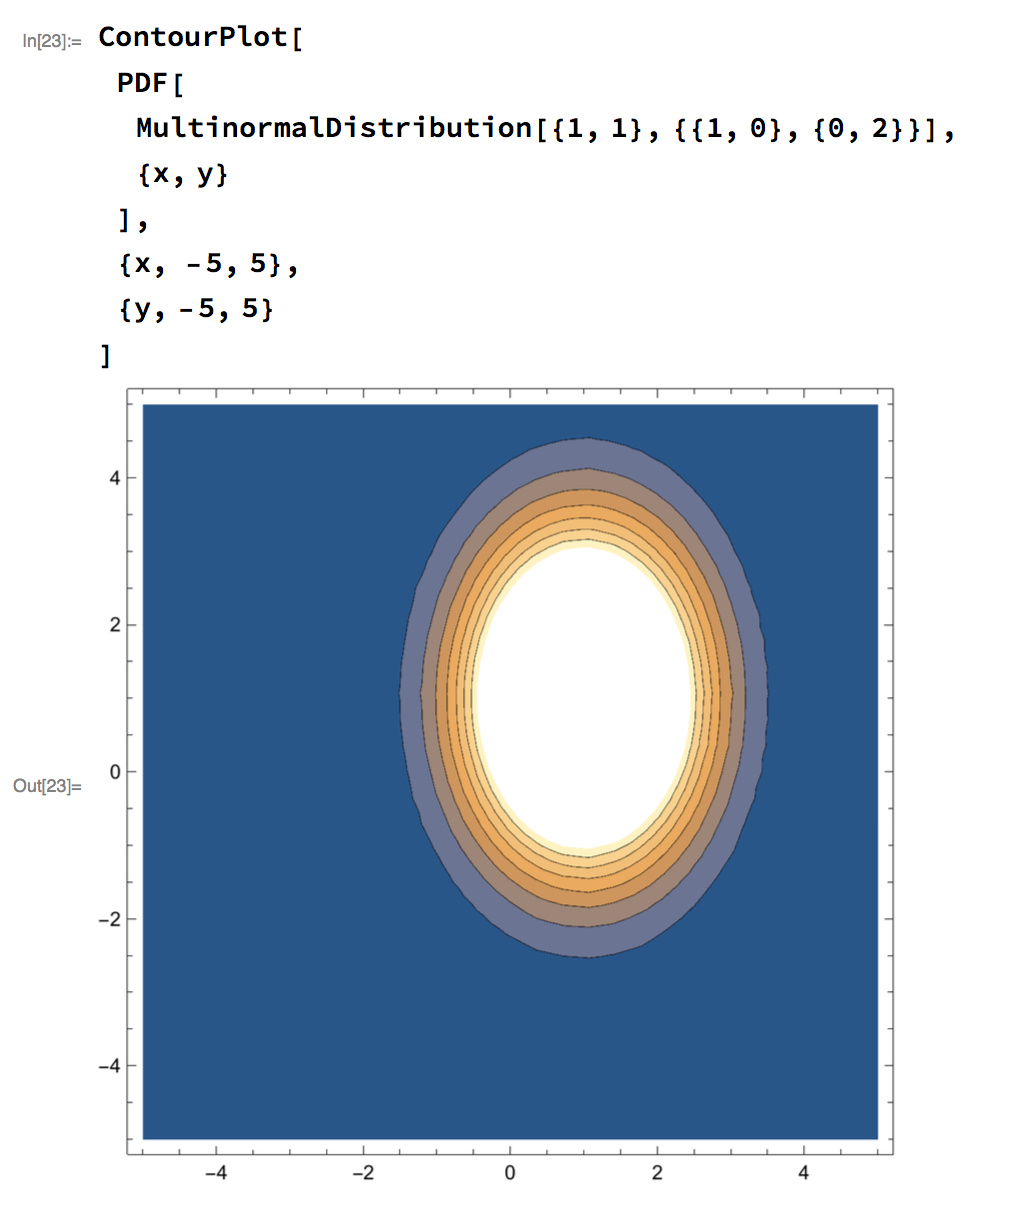
\includegraphics[width=300pt]{img/hw03_2a.png}
    \end{mdframed}
    \newpage
    \item $f(\mu, \Sigma)$, where $\mu = \begin{bmatrix}-1 \\ 2 \end{bmatrix}$ and $\Sigma = \begin{bmatrix} 2 & 1  \\ 1 & 3 \end{bmatrix}$.
    \begin{mdframed}
      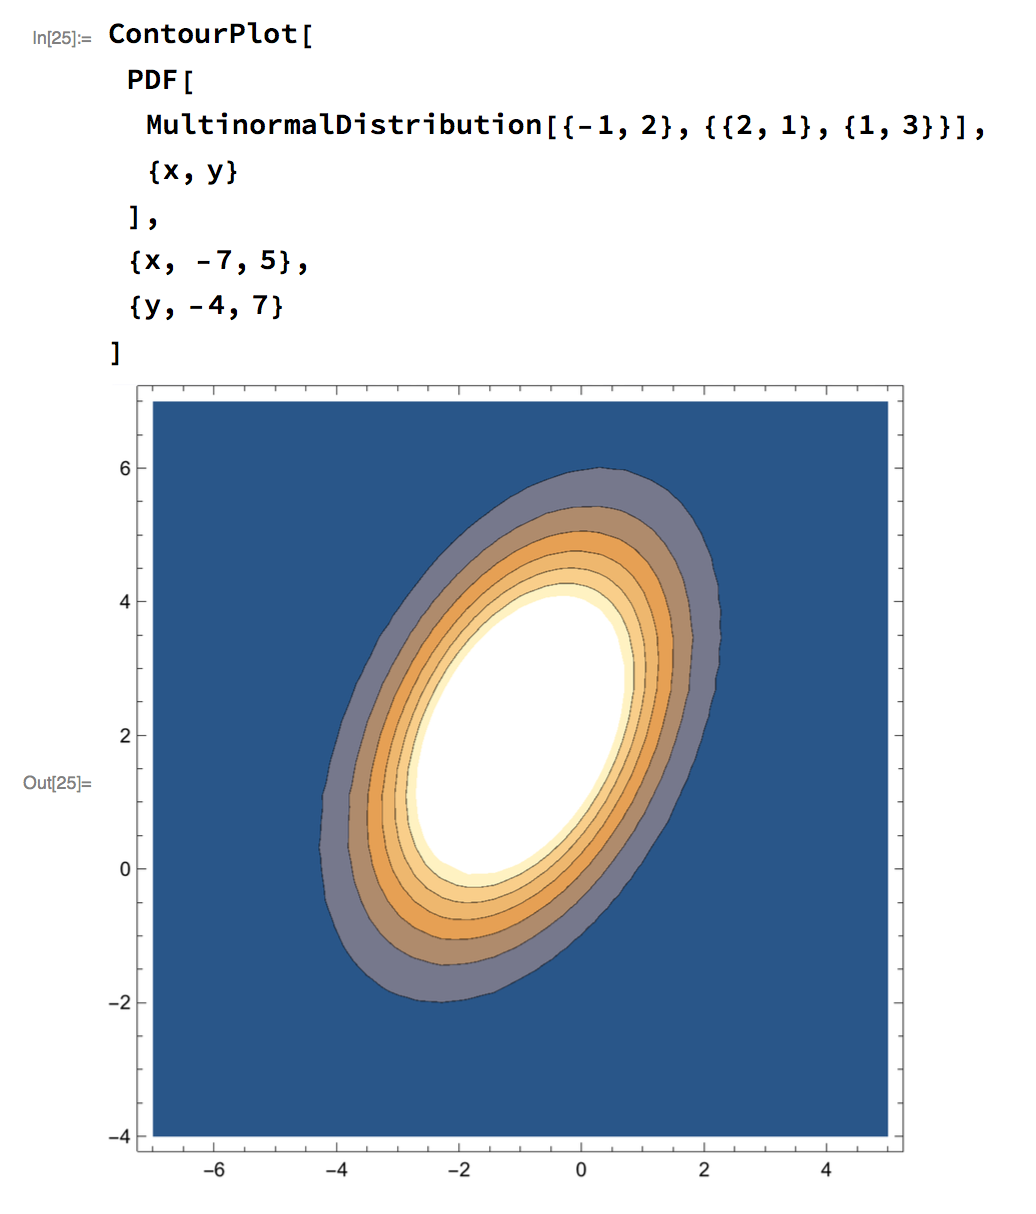
\includegraphics[width=300pt]{img/hw03_2b.png}
    \end{mdframed}

    \newpage
    \item $f(\mu_1, \Sigma_1) - f(\mu_2, \Sigma_2)$, where $\mu_1 = \begin{bmatrix} 0 \\ 2 \end{bmatrix}, \mu_2 = \begin{bmatrix} 2 \\ 0 \end{bmatrix}$ and $\Sigma_1 = \Sigma_2 = \begin{bmatrix} 2 & 1 \\ 1 & 1 \end{bmatrix}$.
    \begin{mdframed}
      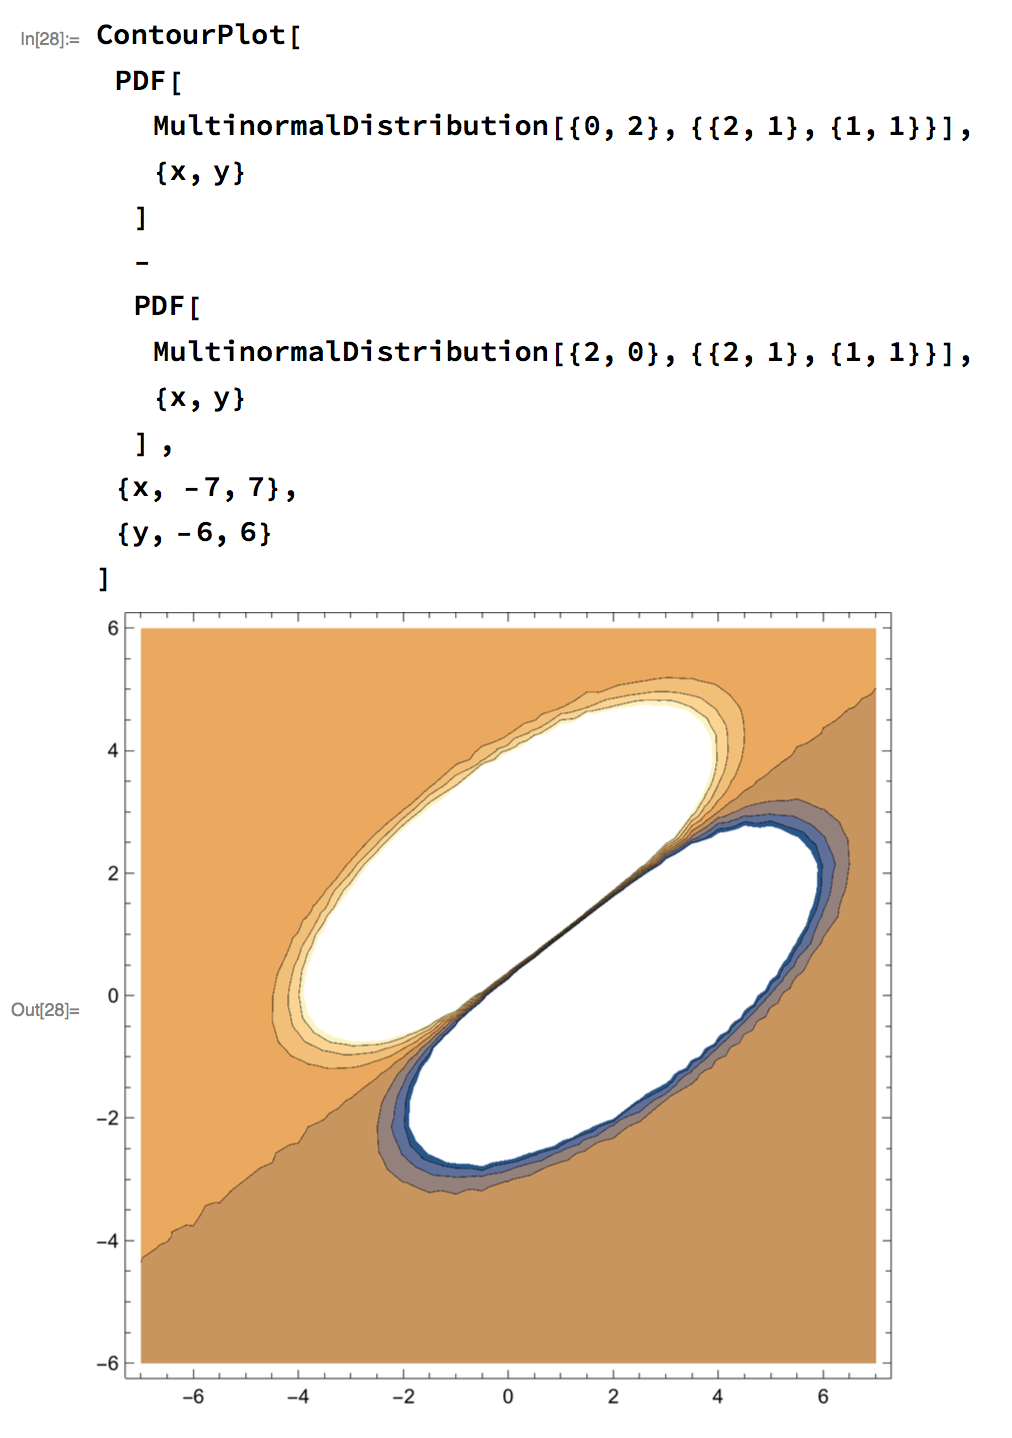
\includegraphics[width=300pt]{img/hw03_2c.png}
    \end{mdframed}

    \newpage
    \item $f(\mu_1, \Sigma_1) - f(\mu_2, \Sigma_2)$, where $\mu_1 = \begin{bmatrix} 0 \\ 2 \end{bmatrix}, \mu_2 = \begin{bmatrix} 2 \\ 0 \end{bmatrix}, \Sigma_1 = \begin{bmatrix} 2 & 1 \\ 1 & 1 \end{bmatrix}$ and $\Sigma_2 = \begin{bmatrix} 2 & 1 \\ 1 & 3 \end{bmatrix}$.
    \begin{mdframed}
      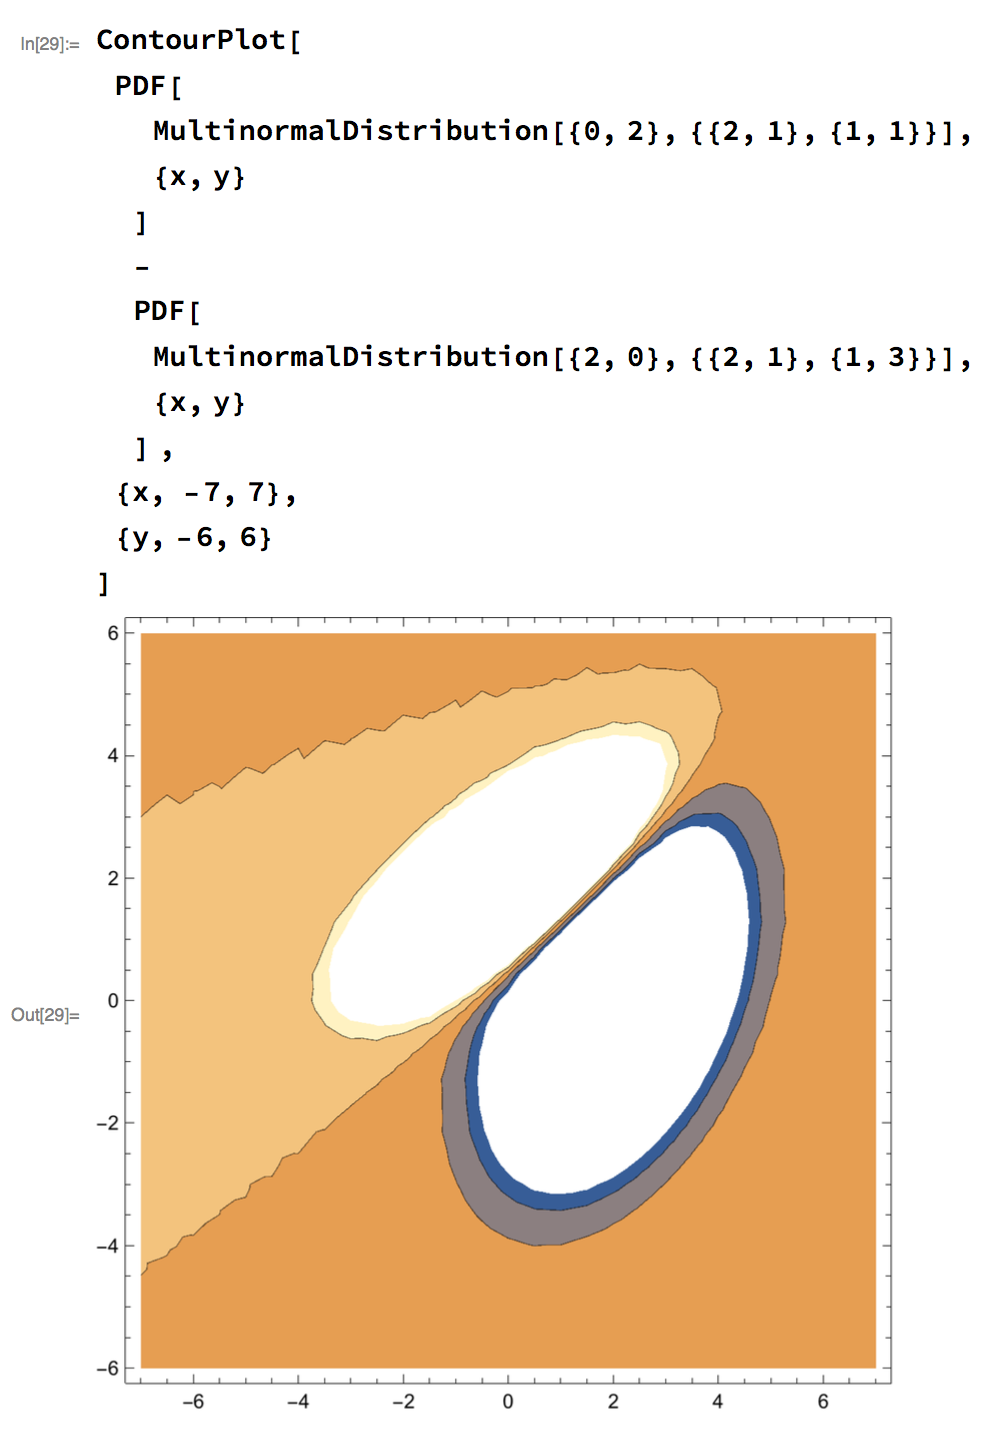
\includegraphics[width=300pt]{img/hw03_2d.png}
    \end{mdframed}

    \newpage
    \item $f(\mu_1, \Sigma_1) - f(\mu_2, \Sigma_2)$, where $\mu_1 = \begin{bmatrix} 1 \\ 1 \end{bmatrix}, \mu_2 = \begin{bmatrix} -1 \\ -1 \end{bmatrix}, \Sigma_1 = \begin{bmatrix} 2 & 0 \\ 0 & 1 \end{bmatrix}$ and $\Sigma_2 = \begin{bmatrix} 2 & 1 \\ 1 & 2 \end{bmatrix}$.
    \begin{mdframed}
      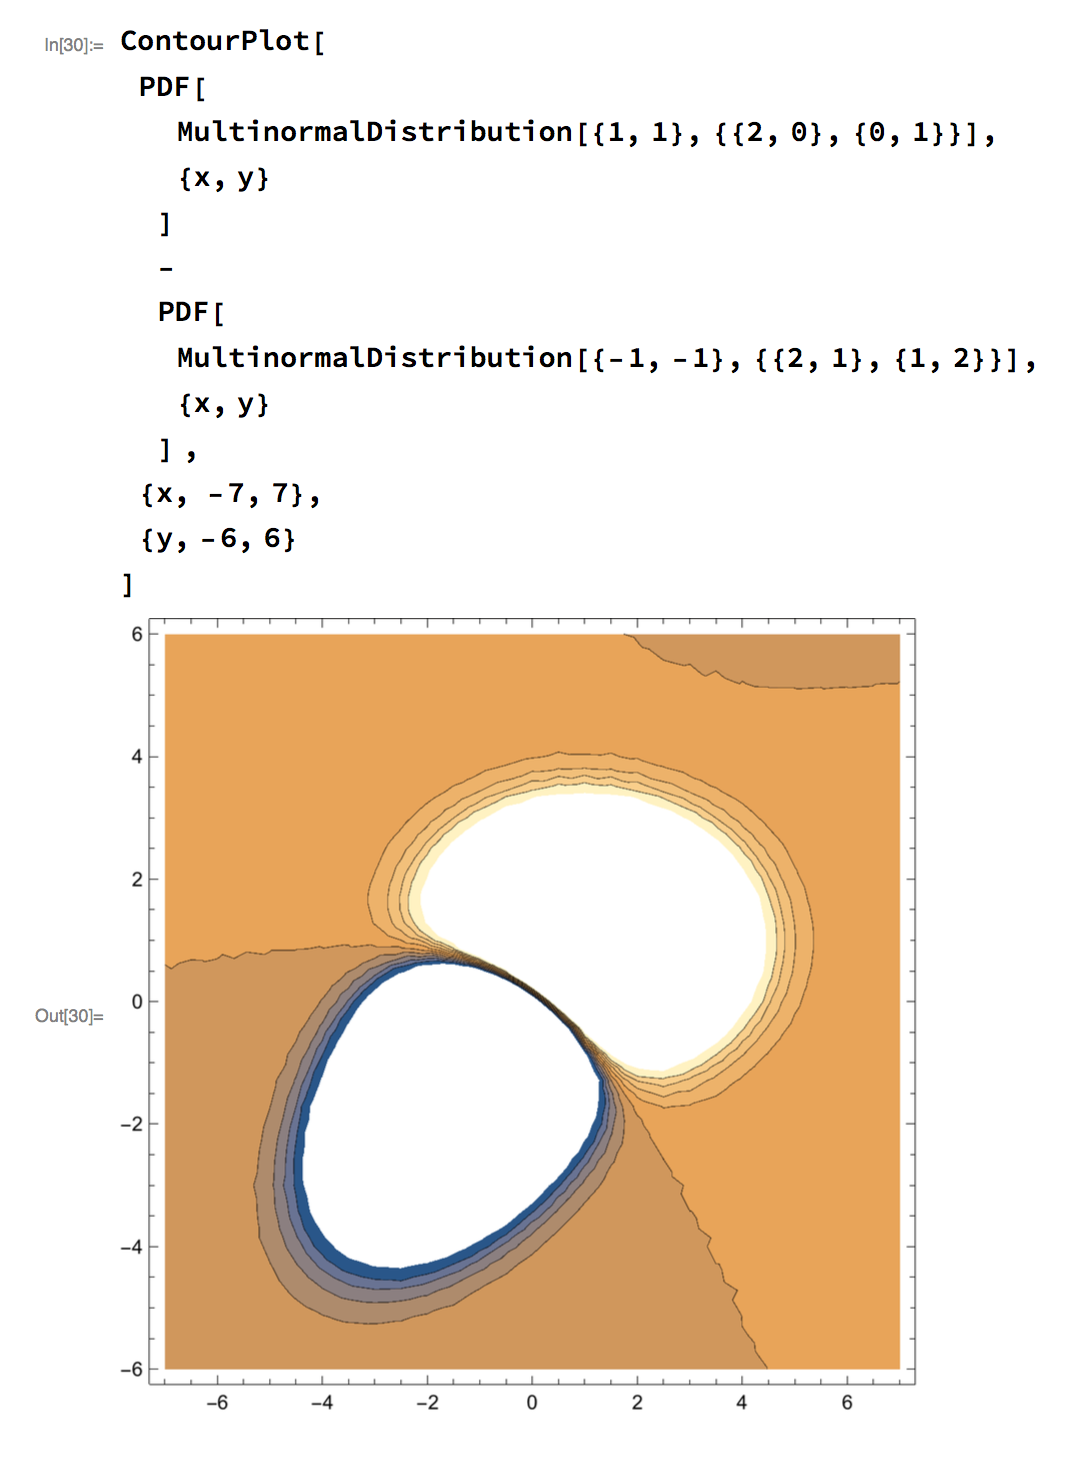
\includegraphics[width=300pt]{img/hw03_2e.png}
    \end{mdframed}

\end{enumerate}

\newpage
\subsection{Eigenvectors of the Gaussian Covariance Matrix}
Consider two one-dimensional random variables $X_1 \sim \N(3, 9)$ and $X_2 \sim \frac{1}{2}X_1 + \N(4, 4)$, where $\N(\mu, \sigma^2)$  is a Gaussian distribution with mean $\mu$ and variance $\sigma^2$. In software, draw $N = 100$ random two-dimensional sample points from $(X_1, X_2)$ such that the $i$th value sampled from $X_2$ is calculated based on the $i$th value sampled from $X_i$.
\begin{enumerate}[label=(\alph*)]
  \item
  \begin{mdframed}
    \begin{minted}{python}
      from numpy.random import normal

      X1 = normal(3, 3, 100)
      X2 = X1/2 + normal(4, 2, 100)
      X = np.stack([X1, X2], axis=1)
      n, d = X.shape
    \end{minted}
  \end{mdframed}
\item Compute the mean (in $\R^2$) of the sample.
  \begin{mdframed}
    \begin{minted}{python}
      mu = X.mean(axis=0)
    \end{minted}
  \end{mdframed}

\item Compute the $2 \times 2$ covariance matrix of the sample.
  \begin{mdframed}
    \begin{minted}{python}
      Sigma = (X - mu).T @ (X - mu) / (n * d)
    \end{minted}
  \end{mdframed}

\item Compute the eigenvectors and eigenvalues of this covariance matrix.
  \begin{mdframed}
    \begin{minted}{python}
      from numpy.linalg import eigh
      evals, evecs = eigh(Sigma)
    \end{minted}
  \end{mdframed}

\newpage
\item On a two-dimensional grid with a horizontal axis for $X_1$ with range $[-15, 15]$ and a vertical axis for $X_2$ with range $[-15, 15]$, plot
  \begin{enumerate}[label=(\roman*)]
  \item all $N=100$ data points, and
  \item arrows representing both covariance eigenvectors. The eigenvector arrows should originate at the mean and have magnitudes equal to their corresponding eigenvalues.
  \end{enumerate}
  \begin{mdframed}
    \begin{minted}{python}
      fig = plt.figure(figsize=(10,10))
      plt.xlim(-15,15)
      plt.ylim(-15,15)
      plt.scatter(X[:,0], X[:,1])
      arrow_kwargs = dict(fc="k", ec="k", head_width=0.3, head_length=0.5)
      plt.arrow(mu[0], mu[1],
      evecs[:,0][0] * evals[0],
      evecs[:,0][1] * evals[0],
      **arrow_kwargs)
      plt.arrow(mu[0], mu[1],
      evecs[:,1][0] * evals[1],
      evecs[:,1][1] * evals[1],
      **arrow_kwargs)
    \end{minted}
    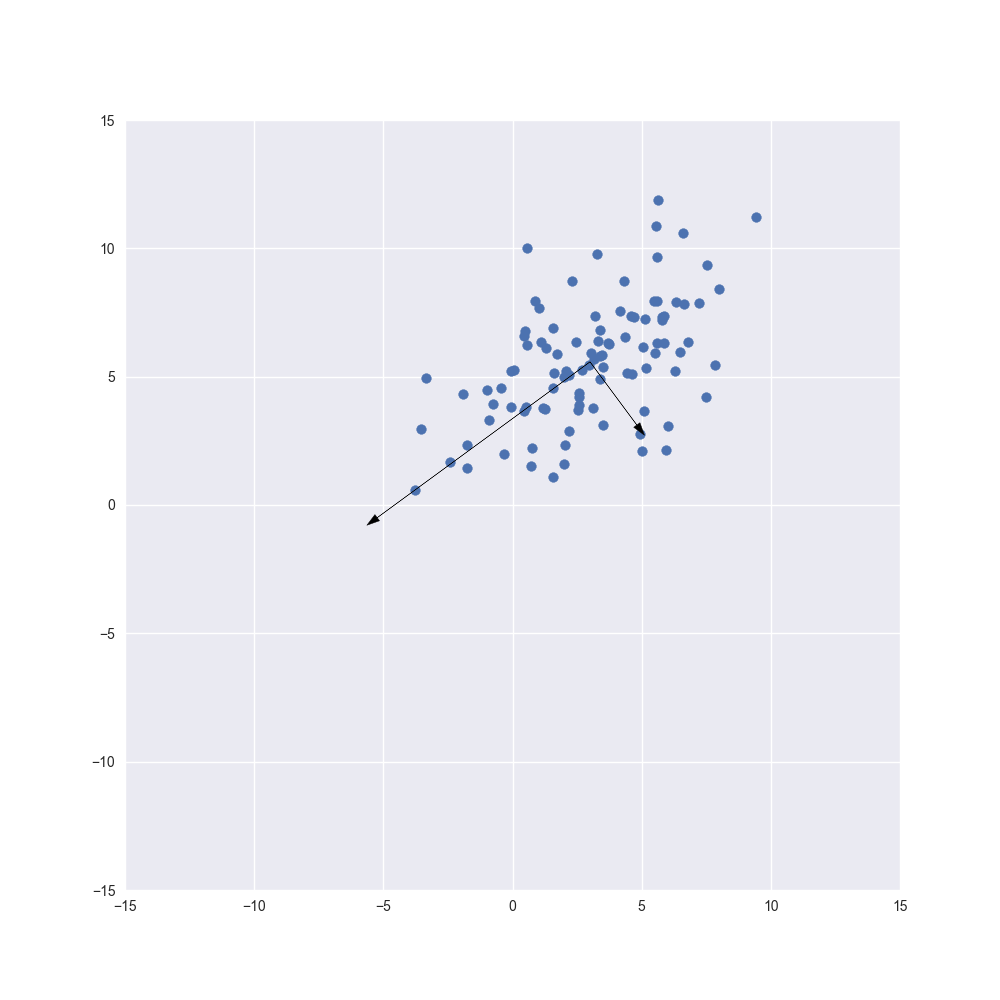
\includegraphics[width=300pt]{img/hw03_3d.png}
  \end{mdframed}

\newpage
\item Let $U = \begin{bmatrix} v_1 & v_2 \end{bmatrix}$ be a $2 \times 2$
  matrix whose columns are the eigenvectors of the covariance matrix, where
  $v_1$ is the eigenvector with the larger eigenvalue. We use $U^{\top}$ as a
  rotation matrix to rotate each sample point from the $(X_1, X_2)$ coordinate
  system to a coordinate system aligned with the eigenvectors. (As
  $U^{\top} = U^{-1}$, the matrix $U$ reverses this rotation, moving back from
  the eigenvector coordinate system to the original coordinate system). Center
  your sample points by subtracting the mean $\mu$ from each point; then rotate
  each point by $U^{\top}$, giving $x_{\text{rotated}} = U^{\top}(x - \mu)$.
  Plot these rotated points on a new two dimensional-grid, again with both axes
  having range $[-15, 15]$.
  \begin{mdframed}
    \begin{minted}{python}
      U = evecs[:,::-1]
      X_centered = X - mu
      X_centered_rotated = (U.T @ X_centered.T).T

      fig = plt.figure(figsize=(10,10))
      plt.xlim(-15,15)
      plt.ylim(-15,15)
      plt.scatter(X_centered_rotated[:,0], X_centered_rotated[:,1])
    \end{minted}
    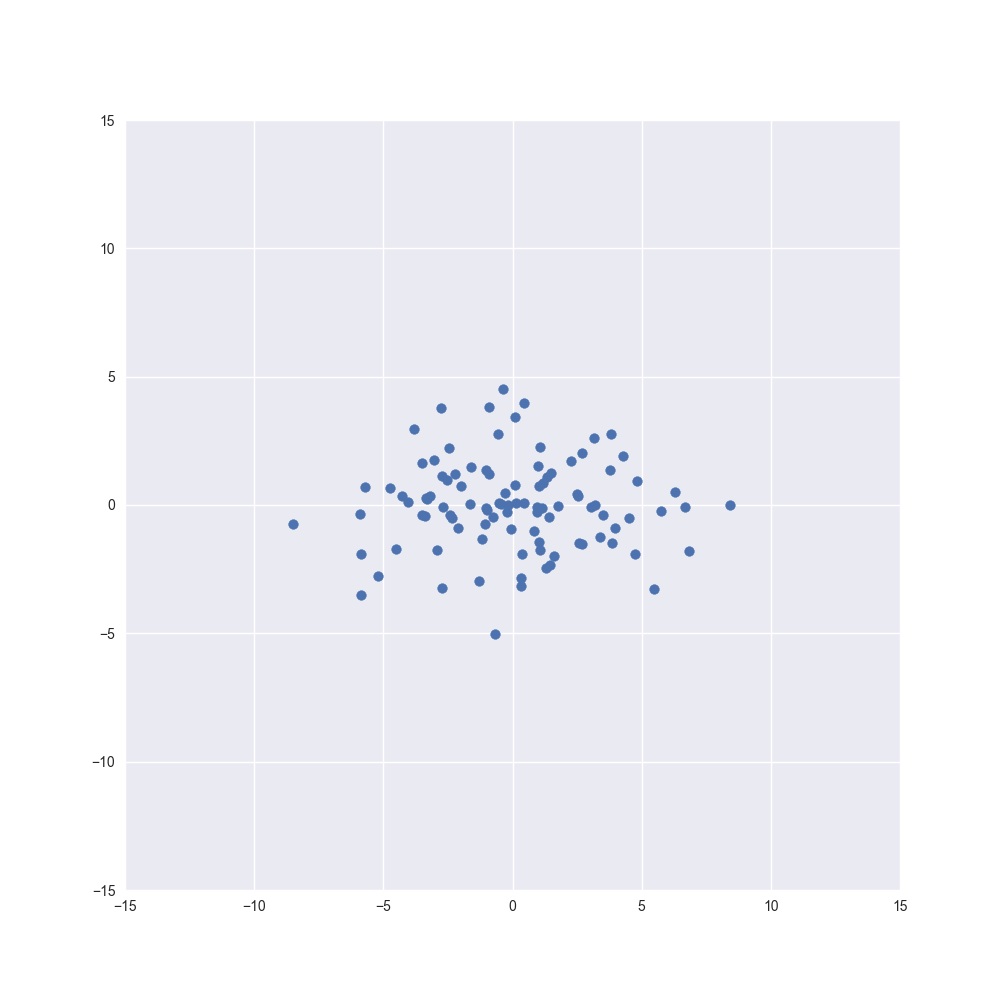
\includegraphics[width=300pt]{img/hw03_3e.png}
  \end{mdframed}

\end{enumerate}

\newpage
\subsection{Maximum Likelihood Estimation}
Let $X_1, \ldots, X_n \in \R^d$ be $n$ sample points drawn independently from a multivariate normal distribution $\N(\mu, \Sigma)$.
\begin{enumerate}[label=(\alph*)]
    \item Suppose the normal distribution has an unknown diagonal covariance matrix
    $$
    \Sigma =
    \begin{bmatrix}
    \sigma_1^2 & & & & \\
    & \sigma_2^2 & & & \\
    & & \sigma_3^2 & & \\
    & & & \ddots & \\
    & & & & \sigma_d^2 \\
    \end{bmatrix}
    $$
    and an unknown mean $\mu$. Derive the maximum likelihood estimates, denoted
    $\hat{\mu}$ and $\hat{\sigma_i}$ for $\mu$ and $\sigma_i$. Show all your
    work.

    (Answer starts on next page)

    \begin{mdframed}
      First, let's get some intuition for the situation: the covariance matrix
      is diagonal, so the isocontours of the PDF of the Gaussian are
      axis-aligned. That means that the PDF can be factored into a product of
      one-dimensional marginal densities: i.e. we can compute the density of a
      sample vector $\vec x$ as the product of densities of its scalar
      components (individual features):
      $\p(\vec x;\vec \mu, \vec \Sigma) = \prod_{j=1}^d \p(\vec x_j; \mu_j,
      \sigma^2_j)$. We therefore expect the estimation problem to be fairly
      straightforward, essentially involving fitting $d$ one-dimensional
      Gaussians independently.

      The likelihood function is
      \begin{align*}
        \L(\mu, \Sigma)
        &= \prod_{i=1}^n \p(X_i;\mu, \Sigma) \\
        &= \prod_{i=1}^n \prod_{j=1}^d \p(\vec X_{ij}; \mu_j, \sigma^2_j) \\
        &= \prod_{i=1}^n \prod_{j=1}^d \frac{1}{(\sqrt{2\pi})^d \sigma_j^d} \exp\(\frac{-(X_{ij} - \mu_j)^2}{2\sigma_j^2}\), \\
      \end{align*}
      giving the log-likelihood function
      \begin{align*}
        \l(\mu, \Sigma)
        &= \sum_{i=1}^n \sum_{j=1}^d -d\log\sigma_j - \frac{(X_{ij} - \mu_j)^2}{2\sigma_j^2} + \constant \\
        &= \sum_{j=1}^d -nd\log\sigma_j - \frac{1}{2\sigma_j^2} \sum_{i=1}^n  (X_{ij} - \mu_j)^2  + \constant. \\
      \end{align*}
      Fix a particular feature $j$. The partial derivatives with respect to the
      mean and variance parameter for that feature are
      \begin{align*}
        \dldmuj &= \frac{1}{\sigma^2_j}\sum_{i=1}^n(X_{ij} - \mu_j) = \frac{1}{\sigma^2_j}\(-n\mu_j + \sum_{i=1}^nX_{ij}\)\\
        \dldsigmaj &= -\frac{nd}{\sigma_j} + \frac{1}{\sigma_j^3} \sum_{i=1}^n  (X_{ij} - \mu_j)^2.
      \end{align*}
      To find the MLE $\hat \mu_j$ we set the partial derivative equal to zero
      and solve for $\mu$:
      \begin{align*}
        \dldmuj = 0
        &\implies -n\hat \mu_j + \sum_{i=1}^nX_{ij} = 0\\
        &\implies \hat \mu_j = \frac{1}{n}\sum_{i=1}^nX_{ij}.
      \end{align*}
      To find the MLE $\hat \sigma_j$ we set the partial derivative equal to
      zero, set $\mu_j = \hat \mu_j$, and solve for $\sigma$:
      \begin{align*}
        \dldsigmaj = 0
        &\implies -nd + \frac{1}{\hat \sigma_j^2} \sum_{i=1}^n  (X_{ij} - \hat \mu_j)^2 = 0 \\
        &\implies \hat \sigma_j^2 = \frac{1}{nd}\sum_{i=1}^n  (X_{ij} - \hat \mu_j)^2.
      \end{align*}
      (Why is it valid to substitute $\hat \mu_j$ for $\mu_j$?)
    \end{mdframed}

    \begin{mdframed}
      To verify that these critical points are indeed maxima, we note first
      that $\l(\mu, \Sigma)$ is a quadratic in $\mu$, in which the sign of
      $\mu_j$ is negative. Therefore it is a concave-down quadratic in $\mu_j$
      and has only a maximum; no minimum.

      For $\sigma$ we compute the second partial derivative,
      \begin{align*}
        \ddldsigmajsigmaj = \frac{nd}{\sigma_j^2} - \frac{3}{\sigma_j^4} \SS_j,
      \end{align*}
      where $\SS_j = \sum_{i=1}^n  (X_{ij} - \mu_j)^2$, and evaluate it at the critical point:
      \begin{align*}
        \ddldsigmajsigmaj(\sigma_j)
        &= \frac{(nd)^2}{\SS_j} - \frac{3(nd)^4}{\(\SS_j\)^4} \SS_j\\
        &= \frac{(nd)^2}{\SS_j} - \frac{3(nd)^4}{\(\SS_j\)^3}.\\
      \end{align*}
      (I was expecting to be able to show that $\ddldsigmajsigmaj(\sigma_j)$ is
      negative but I don't seem to be managing to do so.)
    \end{mdframed}

    \newpage
  \item Suppose the normal distribution has a known covariance matrix $\Sigma$
    and an unknown mean $A \mu$, where $\Sigma$ and $A$ are known $d \times d$
    matrices, $\Sigma$ is positive definite, and $A$ is invertible.  Derive the
    maximum likelihood estimate, denoted $\hat{\mu}$, for $\mu$.
    \begin{mdframed}
      % Let's change coordinate system so that the mean of the Gaussian is
      % $\mu$. Clearly we can do this by applying the transformation $A^\1$.  In
      % this coordinate system, the sample points are the rows of
      % $X' = (A^\1X^\T)^\T$ ($A$ is a covariance matrix of a Gaussian, hence
      % symmetric positive definite, hence invertible).

      % The mean of the rows of $X'$ is $A^\1A\mu = \mu$.

      Let $\eta = A\mu$. Then $\hat \eta_j = \frac{1}{n}\sum_{i=1}^nX_{ij}$ as
      above. There is a theorem (the ``invariance property'') regarding MLEs
      which states that $\hat{g(\theta)}$ is $g(\hat \theta)$, where $\hat~$
      denotes MLE.

      We know $\hat{A\mu}$. We want $\hat{\mu} = \hat{A^\1A\mu}$. By the
      invariance property for MLEs this is
      $$
      \hat \mu = A^\1\hat{A\mu} = A^\1\frac{1}{n}\sum_{i=1}^nX_{ij}.
      $$
      I'm not entirely sure what requirements this theorem makes of $g$ but I
      am confident that the invertible linear transformation $A^\1$ satisfies
      them.

      Alternatively, without relying on this theorem, I tried to argue from
      first principles, but currently am confused when attempting to compute the
      gradient for $\mu$:

      The likelihood function for $\mu$ is
      \begin{align*}
        \L(\mu)
        &= \prod_{i=1}^n \frac{1}{\(\sqrt{2\pi}\)^d\sqrt{|\Sigma|}}\exp\(-\frac{1}{2}(X_i - A\mu)^\T\Sigma^\1(X_i - A\mu)\),
      \end{align*}
      and the log-likelihood function is
      \begin{align*}
        \l(\mu)
        &= -\frac{1}{2}\sum_{i=1}^n (X_i - A\mu)^\T\Sigma^\1(X_i - A\mu) + \constant.
      \end{align*}
      % The first derivative with respect to $\mu$ is
      % \begin{align*}
      %   \dldmu = \sum_{i=1}^n (X_i - A\mu)^\T\Sigma^\1A
      % \end{align*}

      Let $\dot X_i = X_i - A\mu$. Then the log-likelihood is the following
      quadratic form (up to an additive constant):
      \begin{align*}
        \l(\mu)
        &= -\frac{1}{2}\sum_{i=1}^n \dot X_i^\T\Sigma^\1 \dot X_i\\
        &= -\frac{1}{2}\sum_{i=1}^n\sum_{j=1}^d\sum_{k=1}^d \(\Sigma^\1\)_{jk} \dot X_{ij} \dot X_{ik}\\
        &= -\frac{1}{2}\sum_{i=1}^n\sum_{j=1}^d\sum_{k=1}^d \(\Sigma^\1\)_{jk} \(X_{ij} - (A\mu)_j\) \(X_{ik} - (A\mu)_k\)\\
        &= -\frac{1}{2}\sum_{j=1}^d\sum_{k=1}^d \(\Sigma^\1\)_{jk} \sum_{i=1}^n (X_{ij} - (A\mu)_j) (X_{ik} - (A\mu)_k)\\
        &= -\frac{1}{2}\sum_{j=1}^d\sum_{k=1}^d \(\Sigma^\1\)_{jk} \sum_{i=1}^n \(X_{ij}X_{ik} - X_{ik}(A\mu)_j - X_{ij}(A\mu)_k + (A\mu)_j(A\mu)_k\)\\
      \end{align*}



    \end{mdframed}

\end{enumerate}

\newpage
\subsection{Covariance Matrices and Decompositions}
As described in lecture, the covariance matrix $\text{Var}(R) \in \R^{d\times d}$ for a random variable $R \in \R^d$ with mean $\mu$ is
$$
\text{Var}(R) = \text{Cov}(R, R) = \E[(R- \mu)(R-\mu)^{\top}] =
\begin{bmatrix}
\Var(R_1) & \Cov(R_1, R_2) & \ldots & \Cov(R_1, R_d) \\
\Cov(R_2, R_1) & \Var(R_2) & & \Cov(R_2, R_d) \\
\vdots & & \ddots & \vdots \\
\Cov(R_d, R_1) & \Cov(R_d, R_2) & \ldots & \Var(R_d)
\end{bmatrix}
$$
where $\Cov(R_i, R_j) = \E[(R_i - \mu_i)(R_j - \mu_j)]$ and $\Var(R_i) = \Cov(R_i, R_i)$. \\

\noindent
If the random variable $R$ is sampled from the multivariate normal distribution $\N(\mu, \Sigma)$ with the PDF
$$ f(x) = \frac{1}{\sqrt{(2\pi)^d |\Sigma|}} e^{((x-\mu)^{\top}\Sigma^{-1}(x-\mu))/2},$$
then $\Var(R) = \Sigma$.\\

\noindent
Given $n$ points $X_1, X_2, \ldots, X_n$ sampled from $\N(\mu, \Sigma)$, we can estimate $\Sigma$ with the maximum likelihood estimator
$$ \hat{\Sigma} = \frac{1}{n} \sum_{i=1}^n (X_i - \mu)(X_i - \mu)^{\top},$$ which is also known as the covariance matrix of the sample
\begin{enumerate}[label=(\alph*)]
\item The estimate $\hat{\Sigma}$ makes sense as an approximation of $\Sigma$
  only if $\hat{\Sigma}$ is invertible. Under what circumstances is
  $\hat{\Sigma}$ not invertible? Make sure your answer is complete; i.e., it
  includes all cases in which the covariance matrix of the sample is
  singular. Express you answer in terms of the geometric arrangement of the
  sample points Xi.
    \begin{mdframed}
      Let $\dot X$ represent the centered data, i.e. $\dot X_i = X_i - \mu$.

      Note that $\hat \Sigma$ is the mean of a collection of $n$ outer product
      matrices $\dot X_i \dot X_i^\T$, where each outer product matrix is
      contributed by a single sample point. Also note that the columns of
      $\dot X_i \dot X_i^\T$ are all scalar multiples of $\dot X_i$.

      $\hat \Sigma$ is invertible if and only if it is full-rank. Full-rank
      means that its columns are linearly independent.

      From this point of view, the following circumstances will lead to
      $\hat \Sigma$ being singular:

      \begin{enumerate}
      \item \textbf{There is only one point.} If $n = 1$ then $\mu = X_1$ and
        $\dot X_1 = \vec 0$, and the outer product is the zero matrix. This is
        singular (e.g. determinant is zero).
      \item \textbf{$d > 1$ and there are only two points.} If $n = 2$ then
        $\mu$ lies on the line connecting the two points, so
        $\dot X_1 = a\dot X_2$ for some scalar $a$. Therefore the columns of
        the sum of the two outer product matrices differ only by a scalar
        multiple.
      \end{enumerate}

      In general, the centered sample vectors $\{\dot X_i: 1 < i \leq n\}$ must
      span $\R^d$. I.e. if the sample vectors lie in an affine hyperplane of
      $\R^d$ then $\hat \Sigma$ will be singular.

    \end{mdframed}

  \item Suggest a way to fix a singular covariance matrix estimator
    $\hat{\Sigma}$ by replacing it with a similar but invertible matrix. Your
    suggestion may be a kludge, but it should not change the covariance matrix
    too much. Note that infinitesimal numbers do not exist; if your solution
    uses a very small number, explain how to calculate a number that is
    sufficiently small for your purposes.
    \begin{mdframed}
      In my code I have used the pseudoinverse function
      \texttt{numpy.linalg.pinv}.
    \end{mdframed}

  \item Consider the normal distribution $\N(0, \Sigma)$ with mean $\mu =
    0$. Consider all vectors of length 1; i.e., any vector $x$ for which
    $|x| =1$. Which vector(s) $x$ of length 1 maximizes the PDF $f(x)$? Which
    vector(s) $x$ of length 1 minimizes $f(x)$? (Your answers should depend on
    the properties of $\Sigma$.) Explain your answer.
    \begin{mdframed}
      Let $\vec v_1, \vec v_2, \ldots, \vec v_n$ be unit-length eigenvectors of
      $\Sigma$, arranged in order of decreasing eigenvalue.

      Note that $f(x)$ is maximum at the mean $\vec 0$ and decreases with
      increasing distance from $\vec 0$. The exact form of this decrease is
      determined by the quadratic form
      $(\vec x - \mu)^\T\Sigma^\1 (\vec x - \mu)$.

      Then the unit vector $x$ that maximizes $f(\vec x)$ is $\vec v_n$. This
      is because the eigenvector with smallest eigenvalue points in the
      direction of least slope of the quadratic form. Similarly, $\vec v_1$ is
      the unit vector that minimizes $f(\vec x)$ because the eigenvector with
      largest eigenvalue points in the direction of greatest slope of the
      quadratic form.
    \end{mdframed}
\end{enumerate}

\newpage
\subsection{Gaussian Classifiers for Digits and Spam}
In this problem, you will build classifiers based on Gaussian discriminant analysis. Unlike Homework 1, you are NOT allowed to use any libraries for out-of-the-box classification (e.g \texttt{sklearn}). You may use anything in \texttt{numpy} and \texttt{scipy}. \\

\noindent
The training and test data can be found on Piazza in the post corresponding to this homework. Don’t use the training/test data from Homework 1, as they have changed for this homework. Submit your predicted class labels for the test data on the Kaggle competition website and be sure to include your Kaggle display name and scores in your writeup. Also be sure to include an appendix of your code at the end of your writeup.

\begin{enumerate}[label=(\alph*)]
\item Taking pixel values as features (no new features yet, please), fit a
  Gaussian distribution to each digit class using maximum likelihood
  estimation. This involves computing a mean and a covariance matrix for each
  digit class, as discussed in lecture. \emph{Tip}: You may, and probably
  should, contrast-normalize the images before using their pixel values. One
  way to normalize is to divide the pixel values of an image by the $l_2$ norm
  of its pixel values.
\item (Written answer) Visualize the covariance matrix for a particular class
  (digit). How do the diagonal terms compare with the off-diagonal terms? What
  do you conclude from this?
    \begin{mdframed}
      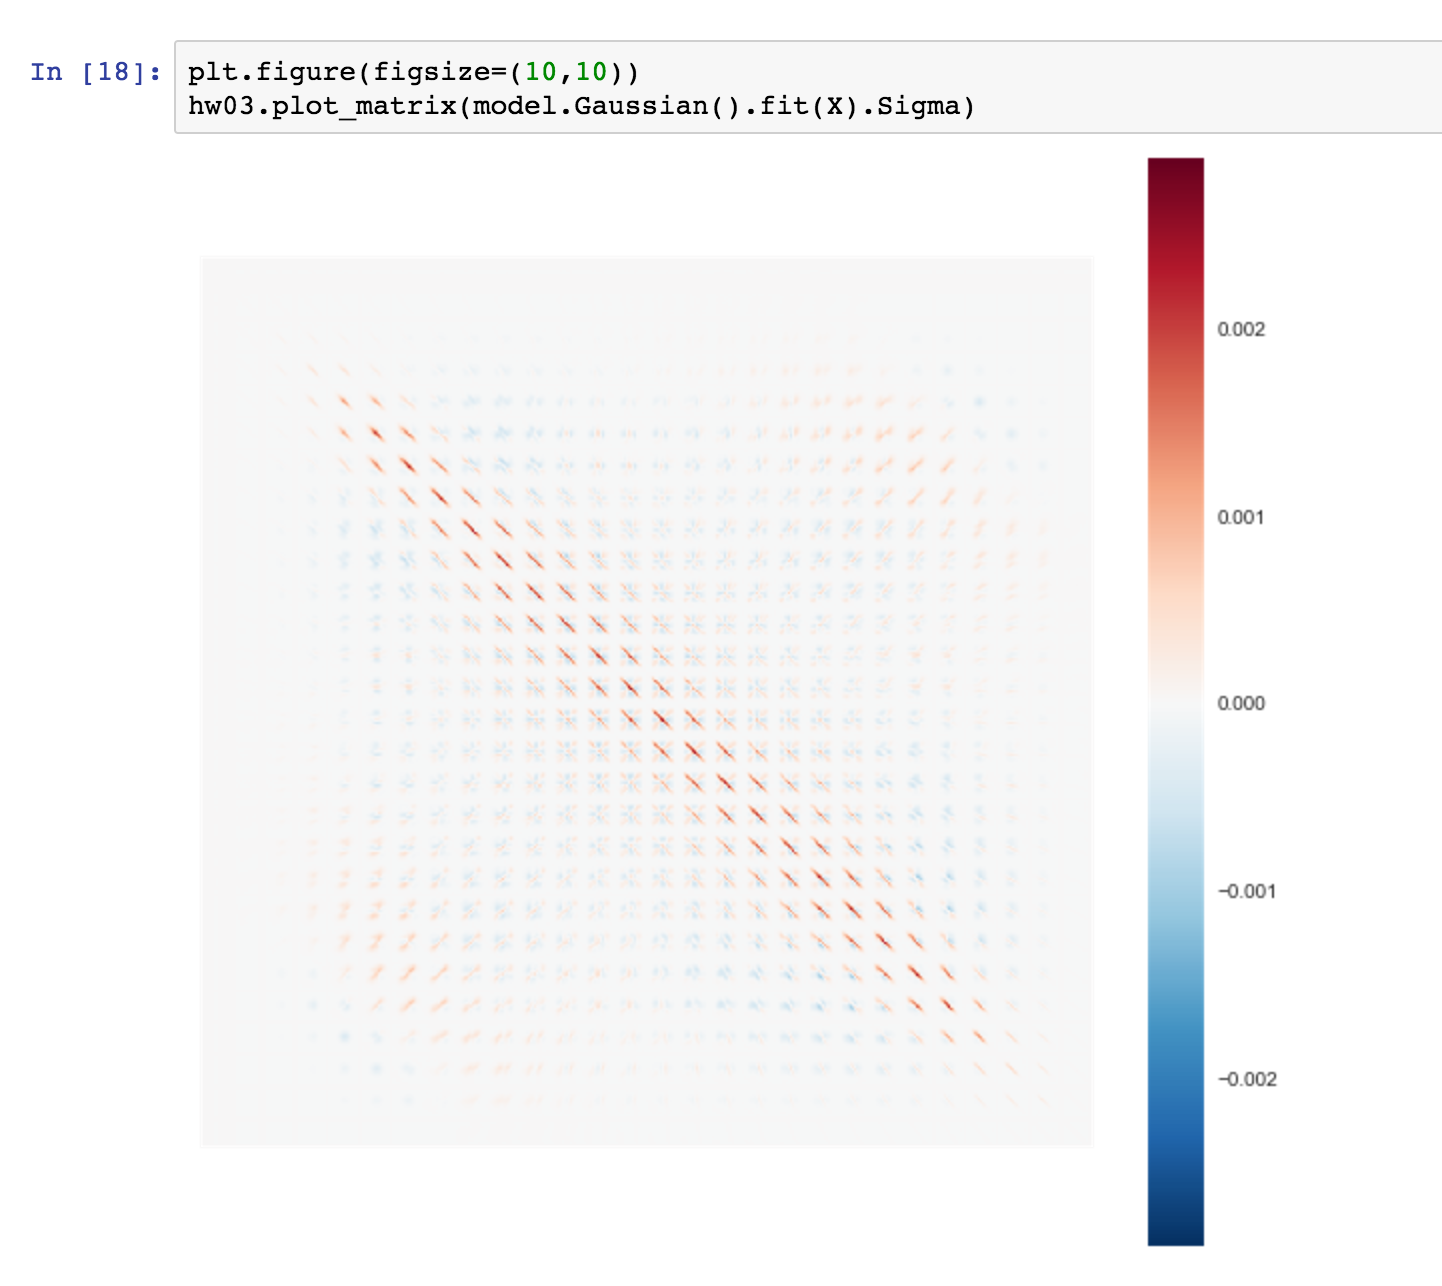
\includegraphics[width=300pt]{img/hw03_6b.png}
    \end{mdframed}

  \item Classify the digits in the test set on the basis of posterior
    probabilities with two different approaches.
    \begin{enumerate}[label=(\roman*)]
        \item Linear discriminant analysis (LDA). Model the class conditional probabilities as Gaussians $\N(\mu_C, \Sigma)$ with different means $\mu_C$ (for class C) and the same covariance matrix $\Sigma$, the average covariance matrix of the 10 classes. \\

        Hold out 10,000 randomly chosen training points for a validation set. Classify each image in the validation set into one of the 10 classes (with a 0-1 loss function). Compute the error rate and plot it over the following numbers of randomly chosen training points: $$[100, 200, 500, 1,000, 2,000, 5,000, 10,000, 30,000, 50,000].$$ (Expect some variance in your error rate when few training points are used.)

        \item Quadratic discriminant analysis (QDA). Model the class conditionals as Gaussians $\N(\mu_C, \Sigma_C)$, where $\Sigma_C$ is the estimated covariance matrix for class C. (If any of these covariance matrices turn out singular, implement the trick you described in Q5.(b). You are welcome to use $k$-fold cross validation to choose the right constant(s) for that trick.) Repeat the same tests and error rate calculations you did for LDA.

        \item  (Written answer.) Which of LDA and QDA performed better? Why?
        \begin{mdframed}
          My QDA implementation is currently incorrect. The unit tests pass for
          1 and 2D cases but when the sample points are higher-dimensional QDA
          is classifying points essentially uniformly at random (around 90\%
          error rate).
          \\\\
          Here are the error rates for my LDA implementation using the provided
          data, with contrast normalization.
          \\\\
          \begin{tabular}{l|l}
            \#{training points}&Error rate\\
            \hline
            100 & 0.51\\
            200 & 0.91\\
            500 & 0.78\\
            1000 & 0.36\\
            2000 & 0.34\\
            5000 & 0.31\\
            10000 & 0.34\\
            30000 & 0.29\\
            50000 & 0.28\\
          \end{tabular}
        \end{mdframed}

      \item Train your best classifier with \texttt{train.mat} and classify the
        images in \texttt{test.mat}. Submit your labels to the online Kaggle
        competition. Record your optimum prediction rate in your
        submission. You are welcome to compute extra features for the Kaggle
        competition. If you do so, please describe your implementation in your
        assignment. Please use extra features \textbf{only} for this portion of
        the assignment. In your submission, include plots of error rate versus
        number of training examples for both LDA and QDA. Also include tables
        giving the error rates (as percentages) for each number of training
        examples for both LDA and QDA. Include written answers where indicated.
        \begin{mdframed}
          0.77 accuracy score for digits; LDA.
        \end{mdframed}

    \end{enumerate}
  \item Next, apply LDA or QDA (your choice) to spam. Submit your test results to the online Kaggle competition. Record your optimum prediction rate in your submission. If you use additional features (or omit features), please describe them. \\

      \emph{Optional:} If you use the defaults, expect relatively low
      classification rates. The TAs suggest using a bag-of-words model. You may
      use third-party packages to implement that if you wish. Also, normalizing
      your vectors might help.

    \begin{mdframed}
      0.71 accuracy score for spam; LDA.
    \end{mdframed}

    \item \emph{Extra for Experts:} Using the \texttt{training\_data} and \texttt{training\_labels} in \texttt{spam.mat}, identify 10 words in your features set corresponding to the maximum and minimum variances. Use $k$-fold cross validation to train your classifier using only 10 variance-maximum words and record your average error rate. Do the same with the 10 minimum-variance words. What do you notice?
    \begin{mdframed} \solution
    % SOLUTION HERE
    \end{mdframed}
\end{enumerate}


\newcommand{\bb}{{\mathbf{b}}}
\newcommand{\bx}{{\mathbf{x}}}
\newcommand{\bmu}{{\mathbf{\mu}}}
\newcommand{\bX}{{\mathbf{X}}}
%\newcommand{\by}{{\mathbf{y}}}
\newcommand{\bY}{{\mathbf{Y}}}
\newcommand{\bz}{{\mathbf{z}}}
\newcommand{\bw}{{\mathbf{w}}}

\newcommand{\auth}[1]{}
\newcommand{\com}[1]{(#1)}
\newcommand{\delete}[1]{}

\newcommand{\todo}[1]{\textcolor{blue}{#1}}
\def\P{{\mathbb P}}
\def\E{{\mathbb E}}
\def\1{{\mathbf 1}}

\newcommand{\argmin}{\mathrm{argmin}}

\section{Homework 4 - Regression}

\subsection{Logistic Regression with Newton's Method}

Consider sample points $X_1, X_2, \ldots, X_n \in \mathbb{R}^d$ and
associated values $y_1, y_2, \ldots, y_n \in \{ 0, 1 \}$,
an $n \times d$ design matrix $X = [X_1~~~~\dots~~~~X_n]^{\T}$ and
an $n$-vector $y = [y_1~~~~\dots~~~~y_n]^{\T}$.

If we add $\ell_2$-regularization to logistic regression,
the cost function is
\[
J(w) = \lambda \, |w|^2_2 -
\sum_{i=1}^n \left(y_i \ln s_i + (1-y_i) \ln (1 - s_i) \rule{0pt}{18pt} \right)
\]
where $s_i = s(X_i \cdot w)$, $s(\gamma) = 1 / (1 + e^{- \gamma})$, and
$\lambda > 0$ is the regularization parameter.
As in lecture, the vector $s = [s_1~~~~\dots~~~~s_n]^{\T}$ is
a useful shorthand.

In this problem, you will use Newton's method to minimize this cost function
on the four-point, two dimensional training set
\[
X = \begin{bmatrix} 0 &3 \\ 1& 3\\ 0 &1\\ 1 &1 \end{bmatrix},
\hspace{1in}
y = \begin{bmatrix} 1\\1\\0\\0 \end{bmatrix}.
\]
You may want to draw these points on paper to see what they look like.
The $y$-vector implies that the first two sample points are in class $1$, and
the last two are in class $0$.

These sample points cannot be separated by a decision boundary that
passes through the origin.
As described in lecture, append a $1$ to each $X_i$ vector and
use a weight vector $w \in \mathbb{R}^3$ whose last component is
the bias term (the term we call $\alpha$ in lecture).

\begin{enumerate}
\item
Derive the gradient of the cost function $J(w)$.
Your answer should be a simple matrix-vector expression.
Do NOT write your answer in terms of the individual components of
the gradient vector.

\begin{comment}
\begin{mdframed}
\textbf{Initial verbose version}:

The gradient of the cost function is
\begin{align*}
  \nabla J(\w) = \lambda \nabla |\w|^2 - \sum_i
  y_i     \nabla \ln s_i(\w) +
  (1-y_i) \nabla \ln(1 - s_i(\w)).
\end{align*}
Let's compute the three derivatives separately.
\hlinee
First the regularization term:
\begin{align*}
  \nabla |\w|^2 = \nabla \sum_{j=1}^d w_j^2 = \cvecccc{2w_1}{\vdots}{2w_d}{2\alpha} = 2\w.
\end{align*}
\hlinee
Next $\ln s_i(\w)$. The partial derivative with respect to one component $w_j$ is
\begin{align*}
  \partiald{\ln s_i(\w)}{w_j}
  = \frac{1}{s_i(\w)} \partiald{s_i(\w)}{w_j}
\end{align*}
and the partial derivative of the logistic function is
\begin{align*}
  \partiald{s_i(\w)}{w_j} &= \partiald{~(1 + e^{-\w \cdot \x_i})^{-1}}{w_j} \\
  &= -(1 + e^{-\w \cdot \x_i})^{-2} (-x_{ij})e^{-\w\cdot\x_i} \\
  &= x_{ij}\frac{e^{-\w\cdot\x_i}}{(1 + e^{-\w \cdot \x_i})^2} \\
  &= x_{ij}s_i(\w)(1 - s_i(\w)),
\end{align*}
so putting the last two results together gives
\begin{align*}
  \partiald{\ln s_i(\w)}{w_j} = x_{ij}(1 - s_i(\w)),
\end{align*}
and therefore the gradient of $\ln s_i(\w)$ is
\begin{align*}
  \nabla \ln s_i(\w) =
\cvecccc
{\partiald{\ln s_i(\w)}{w_1}}
{\vdots}
{\partiald{\ln s_i(\w)}{w_d}}
{\partiald{\ln s_i(\w)}{\alpha}}
=
\cvecccc
{x_{i1}(1 - s_i(\w))}
{\vdots}
{x_{id}(1 - s_i(\w))}
{1 - s_i(\w)}
= (1 - s_i(\w))\x_i.
\end{align*}
\hlinee
Now $\ln(1 - s_i(\w))$. We've already computed $(s_i(\w))'$, so
\begin{align*}
  \partiald{\ln \(1 - s_i(\w)\)}{w_1}
  &= \frac{1}{1 - s_i(\w)}(-1)x_{ij}s_i(\w)(1 - s_i(\w)) \\
  &= -x_{ij}s_i(\w),
\end{align*}
and
\begin{align*}
  \nabla \ln (1 - s_i(\w)) =
\cvecccc
{-x_{i1}s_i(\w)}
{\vdots}
{-x_{id}s_i(\w)}
{-s_i(\w)} =
-s_i(\w)\x_i.
\end{align*}
\hlinee
Finally, putting the three derivatives together gives the gradient of the cost function:
\begin{align*}
  \nabla J(\w)
  &= \lambda \nabla |\w|^2 - \sum_i
  y_i     \nabla \ln s_i(\w) +
  (1-y_i) \nabla \ln(1 - s_i(\w)) \\
  &= 2\lambda\w - \sum_i y_i (1 - s_i(\w))\x_i - (1 - y_i) s_i(\w)\x_i \\
  &= 2\lambda\w - \sum_i y_i\x_i - s_i(\w)\x_i \\
  &= 2\lambda\w - \X^\T\y - \X^\T s(\X\w) \\
  &= 2\lambda\w - \X^\T(\y - s(\X\w)),
\end{align*}
where
$s(\X\w) = \cveccc{1/(1+e^{-\X_1\cdot\w})}{\vdots}{1/(1+e^{-\X_n\cdot\w})}$
contains the predicted values (class probability) for each sample point, given
parameters $\w$.
\end{mdframed}
\end{comment}

\begin{comment}
\begin{mdframed}
\textbf{Second version, not using chain rule}:
First note that
\begin{align*}
  \partiald{s_i(\w)}{w_j} &= \partiald{~(1 + e^{-\w \cdot \x_i})^{-1}}{w_j} \\
  &= -(1 + e^{-\w \cdot \x_i})^{-2} (-x_{ij})e^{-\w\cdot\x_i} \\
  &= x_{ij}\frac{e^{-\w\cdot\x_i}}{(1 + e^{-\w \cdot \x_i})^2} \\
  &= x_{ij}s_i(\w)(1 - s_i(\w)),
\end{align*}
and therefore that
\begin{align*}
  \nabla s_i(\w) = s_i(\w)(1 - s_i(\w))\X_i.
\end{align*}
Then the gradient of the cost function is
\begin{align*}
  \nabla J(\w)
  &= \lambda \nabla |\w|^2 - \sum_i
    y_i     \nabla \ln s_i(\w) +
    (1-y_i) \nabla \ln(1 - s_i(\w)) \\
  &= 2\lambda\w - \sum_i
    \frac{y_i}{s_i(\w)} \nabla s_i(\w) -
    \frac{1 - y_i}{1 - s_i(\w)} \nabla s_i(\w) \\
  &= 2\lambda\w - \sum_i \nabla s_i(\w) \(
    \frac{y_i - s_i(\w)}
         {s_i(\w)(1 - s_i(\w))}
\) \\
  &= 2\lambda\w - \sum_i \X_i\(y_i - s_i(\w)\) \\
  &= 2\lambda\w - \X^\T\(\y - s(\X\w)\),
\end{align*}
where
$s(\X\w) = \cveccc{1/(1+e^{-\X_1\cdot\w})}{\vdots}{1/(1+e^{-\X_n\cdot\w})}$
contains the predicted values (class probability) for each sample point, given
parameters $\w$.

We can interpret this expression a bit. $s(\X\w)$ is an $n$-vector containing
the predicted values for each sample point, so $\y - s(\X\w)$ is the error in
the current predicted values, and $\X^\T(\y - s(\X\w))$ is a $d$-vector whose
$j$-th component is large if feature $j$ is correlated with (has a large dot
product with) the current errors. So the steepest direction downhill will tend
to put more weight on features that are correlated with the current error in
the predictions.
\end{mdframed}
\end{comment}


\begin{mdframed}
Note that $s'(\gamma) = \frac{e^{-\gamma}}{(1 + e^{-\gamma})^2} = s(\gamma)(1 - s(\gamma))$.

Let $s_i = s(\x_i^\T\w)$, so that $\grad_\w s_i = \x_i$. We have
\begin{align*}
  J(\w)     &= \lambda |\w|^2 - \sum_i y_i \log s_i + (1 - y_i) \log\(1 - s_i\),
\end{align*}
so
\begin{align*}
\grad J(\w) &= 2\lambda \w - \sum_i \frac{y_i}{s_i}(s_i)(1 - s_i)\x_i + \frac{1 - y_i}{1 - s_i}(-1)(s_i)(1 - s_i)\x_i \\
            &= 2\lambda \w - \sum_i \x_i\(y_i(1 - s_i) - (1 - y_i)s_i\) \\
            &= 2\lambda \w - \sum_i \x_i\(y_i - s_i\) \\
            &= 2\lambda \w - \X^\T\(\y - \s(\X\w)\) ~~~~~~~~~ (d \by 1)
\end{align*}
where $\s: \R^n \to \R^n$ applies $s$ componentwise to the rows.

We can interpret this expression a bit. $s(\X\w)$ is an $n$-vector containing
the predicted values for each sample point, so $\y - s(\X\w)$ is the error in
the current predicted values, and $\X^\T(\y - s(\X\w))$ is a $d$-vector whose
$j$-th component is large if feature $j$ is correlated with (has a large dot
product with) the current errors. So the steepest direction downhill will tend
to put more weight on features that are correlated with the current error in
the predictions.
\end{mdframed}



\item Derive the Hessian of $J(w)$.
Again, your answer should be a simple matrix-vector expression.

\begin{comment}
\begin{mdframed}
\textbf{Second version, not using chain rule}:
Using $\X_{.j}$ to denote the $n$-vector containing the $j$-th feature
values, the $j$-th component of the gradient is
\begin{align*}
  \partiald{J}{w_j} = 2\lambda w_j - \X_{.j}\cdot \y + \X_{.j} \cdot s(\X\w),
\end{align*}
so the $(j,k)$-th entry of the Hessian is
\begin{align*}
  \partiald{}{w_k}\partiald{J}{w_j}
  &= \sum_i x_{ij} \partiald{~s(\x_i\cdot \w)}{w_k} \\
  &= 2\lambda 1_{\{j = k\}} + \sum_i x_{ij} x_{ik} s_i(\w)(1 - s_i(\w)) \\
  &= \X^\T \B \X,
\end{align*}
where $\B$ is an $(n \times n)$ diagonal matrix with
$B_{ii} = s_i(\w)(1-s_i(\w) + 2\lambda$, and $1_{\{\cdot\}}$ is an indicator
function that takes the value 1 when its argument is true and 0 otherwise.
\end{mdframed}
\end{comment}

\begin{mdframed}
The Hessian is the $d \by \d$ matrix of partial derivatives of the gradient,
so we have
\begin{align*}
  \hess J(\w) = 2\lambda\I + \X^\T \Jac \s(\X\w),
\end{align*}
where $\Jac \s$ is the Jacobian matrix of the vector-valued function $\s$.

We can compute the Jacobian using the chain rule. Define $\f(\w) = \X\w$ so now
$\s(\X\w) = (\s \circ \f)(\w)$:
\\\\
\begin{tabular}{l | l | l | l}
  Function         & domain $\to$ range    & Jacobian                               & dim Jacobian \\
  \hline
  $\f(\w) = \X\w$  &$\R^d \rightarrow \R^n$ &$\D\f = \X$                            & $n \by d$\\
  $\s(\z)$         &$\R^n \rightarrow \R^n$ &$\D\s(\z) = \S$ & $n \by n$
\end{tabular}

where $\S$ is a $n \by n$ diagonal matrix with $\S_{ii} = s_i(1 - s_i)$. Now by
the chain rule,
\begin{align*}
%\D_\w \s(\X\w) &= \D_\w \s(\f(\w)) = ((\D_f \s) (\D_\w \f))(\w) = \s(\f(\w))(1 - \s(\f(\w)))^\T \X
\hess J(\w) &= 2\lambda\I + \X^\T \D_\w \s(\X\w) \\
            &= 2\lambda\I + \X^\T (\D_\f \s) (\D_w \f) \\
            &= 2\lambda\I + \X^\T\S\X.  ~~~~~~~~~~~~~~~~~~~~~~ (d \by d)
\end{align*}
\end{mdframed}


\item State the update equation for one iteration of Newton's method for this
  problem.

\begin{mdframed}
The quadratic approximation to the cost function at $\v$ is
\begin{align*}
  q(\w)
  &= J(\v) + (\w - \v)^\T\(\grad J(\v)\) + \frac{1}{2}(\w - \v)^\T \(\hess J(\v)\) (\w - \v).
  % &= J(\w_0) + \\
  % &~~~~2\lambda(\w - \w_0)^\T \w_0 - \\
  % &~~~~(\w - \w_0)^\T\X^\T\(\y - s(\X\w_0)\) + \\
  % &~~~~\frac{1}{2}(\w - \w_0)^\T \X^\T \B|_{\w_0} \X (\w - \w_0) \\
\end{align*}
We want to find the $\w$ that minimizes this. The gradient of this is something
like
\begin{align*}
  \grad q(\w) = \grad J(\v) + \(\hess J(\v)\)\w,
\end{align*}
but that's not quite right. Anyway, from the lecture notes, setting the
gradient equal to zero gives
\begin{align*}
  \w = \v -\(\hess J(\v)\)^{-1} \grad J(\v).
\end{align*}
For our problem, this is (writing $\w^{(l)}$ instead of $\v$ for the value of $\w$ at iteration $l$.)
\begin{align*}
  \w^{(l+1)} = \w^{(l)} -\(2\lambda\I + \X^\T\S\X\)^{-1} \(2\lambda\w^{(l)} - \X^\T\(\y - s(\X\w^{(l)})\)\).
\end{align*}
\end{mdframed}


\item
We are given a regularization parameter of $\lambda = 0.07$ and
a starting point of $\w^{(0)} = \begin{bmatrix} -2 & 1 & 0 \end{bmatrix}^\T$.
\begin{mdframed}
  \begin{minted}{python3}
from numpy import array
from numpy import diag
from numpy import exp
from numpy.linalg import inv


def q1_4():
    X = array([[0, 3, 1],
               [1, 3, 1],
               [0, 1, 1],
               [1, 1, 1]])
    y = array([[1],
               [1],
               [0],
               [0]])
    lambda_ = 0.07

    w0 = array([[-2],
                [ 1],
                [ 0]])

    s0 = logistic(X @ w0)

    w1 = logistic_regression_newton_update(w0, X, y, lambda_)

    s1 = logistic(X @ w1)

    w2 = logistic_regression_newton_update(w1, X, y, lambda_)


def logistic_regression_newton_update(w, X, y, lambda_):
    s = logistic(X @ w)
    gradient = 2 * lambda_ * w - X.T @ (y - s)
    B = diag((s * (1 - s) + 2 * lambda_).ravel())
    hessian = X.T @ B @ X
    return w - inv(hessian) @ gradient


def logistic(z):
    return 1 / (1 + exp(-z))
  \end{minted}
\end{mdframed}

\begin{itemize}
\item[(a)]
State the value of $s^{(0)}$ (the value of $s$ before any iterations).

\begin{mdframed}
\begin{verbatim}
[[ 0.95257413]
 [ 0.73105858]
 [ 0.73105858]
 [ 0.26894142]]
\end{verbatim}
\end{mdframed}


\item[(b)]
State the value of $w^{(1)}$ (the value of $w$ after one iteration).
\begin{mdframed}
\begin{verbatim}
[[ 0.03660748]
 [ 1.77901816]
 [-3.1787346 ]]
\end{verbatim}
\end{mdframed}


\item[(c)]
State the value of $s^{(1)}$.
\begin{mdframed}
\begin{verbatim}
[[ 0.89644368]
 [ 0.89979306]
 [ 0.19786111]
 [ 0.20373548]]
\end{verbatim}
\end{mdframed}


\item[(d)]
State the value of $w^{(2)}$ (the value of $w$ after two iterations).
\begin{mdframed}
\begin{verbatim}
[[-0.84243273]
 [ 1.2968546 ]
 [-1.60471569]]
\end{verbatim}
\end{mdframed}

\end{itemize}
\end{enumerate}


\newpage


\subsection{$\ell_1$- and $\ell_2$-Regularization}


Consider sample points $X_1, X_2, \ldots, X_n \in \mathbb{R}^d$ and
associated values $y_1, y_2, \ldots, y_n \in \mathbb{R}$,
an $n \times d$ design matrix $X = [X_1~~~~\dots~~~~X_n]^{\T}$ and
an $n$-vector $y = [y_1~~~~\dots~~~~y_n]^{\T}$.
For the sake of simplicity, assume that the sample data
has been centered and whitened so that
each feature has mean $0$ and variance $1$ and the features are uncorrelated;
i.e., $X^\T X = nI$.
For this question, we will not use a fictitious dimension nor a bias term;
our linear regression function will be zero for $x = 0$.

Consider linear least-squares regression with
regularization in the $\ell_1$-norm, also known as Lasso.
The Lasso cost function is
\[
J(w) = |Xw - y|^2 +\lambda \, \|w\|_{\ell_1}
\]
where $w \in \mathbb{R}^d$ and $\lambda > 0$ is the regularization parameter.
Let $w^* = \argmin_{w \in \mathbb{R}^d} \, J(w)$ denote
the weights that minimize the cost function.

In the following steps, we will show that whitened training data decouples the features, so that $w^*_i$ is determined by the $i^\mathrm{th}$ feature alone (i.e., column $i$ of the design matrix $X$), regardless of the other features.  This is true for both Lasso and ridge regression.

\begin{enumerate}
\item
We use the notation $X_{*1}, X_{*2}, \ldots, X_{*d}$ to denote column $i$ of the design matrix $X$, which represents the $i^\mathrm{th}$ feature.
(Not to be confused with row $i$ of $X$, the sample point $X_i^\T$.)
Write $J(w)$ in the following form for appropriate functions $g$ and $f$.
\[
J(w) = g(y) + \sum_{i=1}^d f(X_{*i}, w_i, y, \lambda)
\]

\begin{mdframed}
  The cost function is
  \begin{align*}
    J(\w)
    =& |\X\w - \y|^2 + \lambda ||\w||_1 \\
    =& \w^\T\X^\T\X\w - 2y^\T\X\w + \y^\T\y + \lambda ||\w||_1 \\
    =& n\w^\T\w - 2y^\T\X\w + \y^\T\y + \lambda ||\w||_1 ~~~~~~~~~~~~~~~\text{(because $\X^\T\X=n\I$)}.\\
  \end{align*}
Now $\w^\T\w = \sum_{i=1}^d w_i^2$, and $||\w||_1 = \sum_{i=1}^d |w_i|$, and
\begin{align*}
  y^\T\X\w &= (\y^\T\X) \w = \sum_{i=1}^d \X_{*i}^\T ~\y w_i, \\
\end{align*}
so
\begin{align*}
  J(\w) &= g(\y) + \sum_{i=1}^d f(\X_{*i}, w_i, y, \lambda), ~~~~~~~~\text{where}\\
  g(\y) &= \y^\T\y ~~~~~~~~~~~~~~~~~~~~~~~~~~~~~~~~~~~~~~~~~~~~\text{and}\\
  f(\X_{*i}, w_i, \y, \lambda) &= nw_i^2 + \lambda|w_i| - 2\X_{*i}^\T ~\y w_i.
%                              &= |w_i|\(n|w_i| + \lambda\) - 2\X_{*i}^\T ~\y w_i.
\end{align*}
\end{mdframed}

\item
If $w_i^* > 0$, what is the value of $w_i^*$?

\begin{mdframed}
For $w_i \geq 0$, the $i$-th component of $J(\w)$ is
\begin{align*}
  J(\w)_i = nw_i^2 + w_i (\lambda  - 2\X_{*i}^\T ~\y) + \constant.
\end{align*}
so
\begin{align*}
  \partiald{J}{w_i} = 2nw_i + \lambda - 2\X_{*i}^\T ~\y,
\end{align*}
and setting the gradient equal to zero gives
\begin{align*}
  w^*_i =
  \begin{cases}
    \frac{ 2\X_{*i}^\T ~\y - \lambda }{2n}, &\X_{*i}^\T ~\y  > \frac{\lambda}{2}\\
    0,                                     &\text{otherwise}.
  \end{cases}
\end{align*}
\end{mdframed}

\item
If $w_i^* < 0$, what is the value of $w_i^*$?

\begin{mdframed}
For $w_i \leq 0$, the $i$-th component of $J(\w)$ is
\begin{align*}
  J(\w)_i = nw_i^2 - w_i (\lambda  + 2\X_{*i}^\T ~\y) + \constant.
\end{align*}
so
\begin{align*}
  \partiald{J}{w_i} = 2nw_i - \lambda - 2\X_{*i}^\T ~\y,
\end{align*}
and setting the gradient equal to zero gives
\begin{align*}
  w^*_i =
  \begin{cases}
    \frac{ \lambda + 2\X_{*i}^\T ~\y }{2n}, &\X_{*i}^\T ~\y  < -\frac{\lambda}{2}\\
    0,                                     &\text{otherwise}.
  \end{cases}
\end{align*}
\end{mdframed}


\item
Considering parts 2 and 3, what is the condition for $w_i^*$ to be zero?
\begin{mdframed}
  $|\X_{*i}^\T ~\y| \leq \frac{\lambda}{2}$.
\end{mdframed}

\item
Now consider ridge regression, which uses the $\ell_2$ regularization term $\lambda \, |w|^2$.
How does this change the function $f(\cdot)$ from part 1?
What is the new condition in which $w_i^* = 0$?
How does it differ from the condition you obtained in part 4?

\begin{mdframed}
For ridge regression we have
\begin{align*}
  J(\w) &= g(\y) + \sum_{i=1}^d f(\X_{*i}, w_i, y, \lambda), ~~~~~~~~~~~\text{where}\\
  f(\X_{*i}, w_i, \y, \lambda) &= (n+\lambda)w_i^2 - 2\X_{*i}^\T ~\y w_i,
\end{align*}
and $g$ is as above. So
\begin{align*}
  \partiald{J}{w_i} = 2(n + \lambda)w_i - 2\X_{*i}^\T ~\y,
\end{align*}
and
\begin{align*}
  w^*_i = \frac{ \X_{*i}^\T ~\y }{n + \lambda}.
\end{align*}
So the weight for the $i$-th feature is zero if and only if
$\X_{*i}^\T ~\y = 0$, i.e. the $n$-vector containing the $i$-th feature is
orthogonal to the observed training values $\y$.

This is in contrast to Lasso, for which the $i$-th feature receives a weight of
zero if $|\X_{*i}^\T ~\y| \leq \frac{\lambda}{2}$, i.e. if the dot product of
the $i$-th feature with the training values $\y$ falls below $\lambda/2$.

This result is consistent with the general notion that Lasso tends to set some
weights to exactly zero whereas ridge regression would set them to a small but
usually non-zero value.
\end{mdframed}

\end{enumerate}


\newpage


\subsection{Regression and Dual Solutions}


\begin{enumerate}[a)]

\item
For a vector $w$, derive $\nabla \, |w|^4$.
Then derive $\nabla_w \, |Xw - y|^4$.

\begin{mdframed}
Suppose $\w \in \R^d$. Then $|\w|^4 \in \R$ is
\begin{align*}
  |\w|^4 = \(\sum_{j=1}^d w_j^2\)^2 = \sum_{j=1}^d \sum_{k=1}^d w_j^2w_k^2.
\end{align*}
Now consider the $j$-th component. Viewed as a function of $\w_j$, we have
\begin{align*}
  |\w|^4 &= w_j^4 + 2w_j^2\sum_{k \neq j} w_k^2 + \constant
\end{align*}
therefore
\begin{align*}
  \partiald{|\w|^4}{w_j}
  &= 4w_j^3 + 4w_j\sum_{k \neq j} w_k^2 \\
  &= 4|\w|^2w_j
\end{align*}
so
\begin{align*}
  \grad_\w |\w|^4 = 4|\w|^2\w.
\end{align*}
\end{mdframed}
~\\
\begin{mdframed}
Now let $|\X\w - \y|^4 = (g \circ f)(\w)$, where
\begin{align*}
  &f: \R^d \rightarrow \R^n     &f(\w) = \X\w - \y \\
  &g: \R^n \rightarrow \R       &g(\vec z) = |\vec z|^4.
\end{align*}
The chain rule states that $\grad (g \circ f) = (Df)^\T \grad g$, where $Df$
is the Jacobian matrix of first partial derivatives of $f$. We have
$\grad g(\z) = 4|\z|^2\z$ and $Df = \X$, so
\begin{align*}
  \grad_w |\X\w - \y|^4
  &= (Df)^\T \grad g \\
  &= 4|\X\w - \y|^2\X^\T (\X\w - \y) \\
  &= 4|\X\w - \y|^2\X^\T\X\w - \X^\T\y
\end{align*}


\end{mdframed}

\item
Consider sample points $X_1, X_2, \ldots, X_n \in \mathbb{R}^d$ and
associated values $y_1, y_2, \ldots, y_n \in \mathbb{R}$,
an $n \times d$ design matrix $X = [X_1~~~~\dots~~~~X_n]^{\T}$ and
an $n$-vector $y = [y_1~~~~\dots~~~~y_n]^{\T}$, and
the regularized regression problem
\[
w^* = \argmin_{w \in \R^d} \; |Xw - y|^4 + \lambda \, |w|^2,
\]
which is similar to ridge regression, but we take the fourth power
of the error instead of the squared error.
(It is not possible to write the optimal solution $w^*$ as
the solution of a system of linear equations, but
it can be found by gradient descent or Newton's method.)

Show that the optimum $w^*$ is unique.
By setting the gradient of the objective function to zero,
show that $w^*$ can be written as
a linear combination $w^* = \sum_{i=1}^n a_i X_i$ for some scalars
$a_1, \ldots, a_n$.
Write the vector $a$ of dual coefficients in terms of $X$, $y$, and
the optimal solution $w^*$.

\begin{mdframed}
The objective function $J(\w)$ is
\begin{align*}
  |\X\w - \y|^4 + \lambda |\w|^2
  &= \((\X\w - \y) \cdot (\X\w - \y)\)^2 + \lambda |\w|^2 \\
  &= \(\w^T\X^\T\X\w - 2 \w^\T\X^\T\y + \y^\T \y\)^2 + \lambda |\w|^2 \\
\end{align*}

I think this objective function is convex in $\w$, but I'm not sure how to show
that. Basically, I think $\w^T\X^\T\X\w$ is a convex function of $\w$ since
$\X^\T\X$ is positive definite, and $2\w^\T\X^\T\y$ is also a convex function
of $\w$, and the sum of convex functions is convex, and the square of a convex
function is convex, so the whole expression is convex. Being convex in $\w$
means that there is a unique minimum at $\w^*$.

The gradient of the objective function $J(\w)$ is
\begin{align*}
\grad_\w J(\w) = 4|\X\w - \y|^2\X^\T\X\w - \X^\T\y + 2\lambda \w.
\end{align*}
Setting this equal to zero gives
TODO: LaTeX error
% \begin{align*}
%   4|\X\w^* - \y|^2\X^\T\X\w^* + 2\lambda \w^* &= \X^\T\y \\
%   4\(\w^*^\T\X^\T\X\w^* - 2\y^\T\X\w^* + \y^\T\y\)\X^\T\X\w^* + 2\lambda \w^* &= \X^\T\y \\
%   4\w^*^\T\X^\T\X\w^* - 2\y^\T\X\w^* + \y^\T\y\)\X^\T\X\w^* + 2\lambda \w^* &= \X^\T\y,
% \end{align*}
but I don't see how to simplify this to show that $w^*$ can be written as a
linear combination $w^* = \sum_{i=1}^n a_i X_i$ for some scalars
$a_1, \ldots, a_n$.
\end{mdframed}

\item Consider the regularized regression problem
\[
w^* = \argmin_{w \in \R^d} \; \frac{1}{n} \sum_{i=1}^n L(w^{\T} X_i, y_i) + \lambda \, |w|^2
\]
where the loss function $L$ is convex in its first argument.
Prove that the optimal solution has the form $w^* = \sum_{i=1}^n a_i X_i$.
If the loss function is not convex, does the optimal solution always have
the form $w^* = \sum_{i=1}^n a_i X_i$?
Justify your answer.
\end{enumerate}


\newpage


\subsection{Classification + Logistic Regression}

  Daylen is planning the frat party of the semester. He's completely stocked up
  on Franzia. Unfortunately, the labels for 497 boxes (test set) have been
  scratched off, and he needs to quickly find out which boxes contain Red wine
  (label 1) and White wine (label 0). Fortunately, for him the boxes still have
  their Nutrition Facts (features) intact and detail the chemical composition
  of the wine inside the boxes (the description of these features and the
  features themselves are provided in {\tt data.mat}). He also has 6,000 boxes
  with Nutrition Facts and labels intact (train set). Help Daylen figure out
  what the labels should be for the 497 mystery boxes.

\begin{enumerate}
\item Derive and write down the batch gradient descent update equation for
  logistic regression with $\ell_2$ regularization.

\begin{mdframed}
From Q1, the gradient of the cost function is
\begin{align*}
  \nabla J(\w) = 2\lambda\w - \X^\T\(\y - s(\X\w)\),
\end{align*}
where
$s(\X\w) = \cveccc{1/(1+e^{-\X_1\cdot\w})}{\vdots}{1/(1+e^{-\X_n\cdot\w})}$
contains the predicted values (class probability) for each sample point, given
parameters $\w$.

Therefore the batch gradient descent update equation with learning rate
$\epsilon$ at iteration $k$ is
\begin{align*}
  \w^{(k+1)} = \w^{(k)} - \epsilon\(2\lambda\w^{(k)} - \X^\T\(\y - s(\X\w^{(k)})\)\).
\end{align*}

\end{mdframed}


  Choose a reasonable regularization parameter value and a reasonable learning
  rate.  Run your algorithm and plot the cost function as a function of the
  number of iterations.  (As this is batch descent, one ``iteration'' should
  use every sample point once.)

\begin{mdframed}
  My implementation of logistic regression with regularization passes the
  simple 1D test case, but has some numerical problems when used on the real
  data, causing the cost function to not always decrease under gradient
  ``descent''. Therefore I failed to make a Kaggle submission.
\end{mdframed}

\item Derive and write down the stochastic gradient descent update equation for
  logistic regression with $\ell_2$ regularization.  Choose a suitable learning
  rate.  Run your algorithm and plot the cost function as a function of the
  number of iterations---where now each ``iteration'' uses {\em just one}
  sample point.

\begin{mdframed}
The stochastic gradient descent update equation is:

On each iteration:
\begin{enumerate}
\item Sample $i$ from a discrete Uniform distribution on
$1, \ldots, n$.
\item Update $w$ according to
\begin{align*}
  \w^{(k+1)} = \w^{(k)} - \epsilon\(2\lambda\w^{(k)} - \x_i^\T\(\y - s(\x_i^\T\w^{(k)})\)\).
\end{align*}
\end{enumerate}
\end{mdframed}

  Comment on the differences between the convergence of batch and stochastic
  gradient descent.

\item Instead of a constant learning rate $\epsilon$, repeat part 2 where the
  learning rate decreases as $\epsilon \propto 1/t$ for the $t^\mathrm{th}$
  iteration. Plot the cost function vs.\ the number of iterations. Is this
  strategy better than having a constant $\epsilon$?

\item Finally, train your classifier on the entire training set. Submit your
  predictions for the test set to Kaggle. You can only submit twice per day, so
  get started early! In your writeup, include your Kaggle display name and
  score and describe the process you used to decide which parameters to use for
  your best classifier.

\end{enumerate}



\newpage


\subsection{Real World Spam Classification}


\textbf{Motivation}: After taking CS 189 or CS 289A, students should be able to wrestle with ``real-world'' data and problems. These issues might be deeply technical and require a theoretical background, or might demand specific domain knowledge. Here is an example that a past TA encountered.

Daniel (a past CS 189 TA) interned as an anti-spam product manager for an email service provider. His company uses a linear SVM to predict whether an incoming spam message is spam or ham. He notices that the number of spam messages received tends to spike upwards a few minutes before and after midnight. Eager to obtain a return offer, he adds the timestamp of the received message, stored as number of milliseconds since the previous midnight, to each feature vector for the SVM to train on, in hopes that the ML model will identify the abnormal spike in spam volume at night. To his dismay, after testing with the new feature, Daniel discovers that the linear SVM's success rate barely improves.

Why can't the linear SVM utilize the new feature well, and what can Daniel do to improve his results? Daniel is unfortunately limited to a quadratic kernel i.e. the features are at most polynomials of degree 2 over the original variables. This is an actual interview question Daniel received for a machine learning engineering position!

Write a short explanation. This question is open ended, and there can be many correct answers.


\begin{mdframed}
  The way the new feature was defined means that both small and large values
  are associated with being spam. I wonder if it would perform better if
  instead he defined it as:
  \begin{center}
    Absolute value of (timestamp at noon) minus (timestamp of email)
  \end{center}
  although, perhaps the quadratic kernel would already be handling this.

\end{mdframed}

\section{Homework 6 - Neural Networks}
\subsection{Model specification}

\begin{mdframed}
$K$ possible output categories; one hidden layer of $H$ units; $\tanh$
activation in the hidden layer; logistic activation in the output
layer. Notation:

\begin{tabular}{l|l|l|l}
                        &                                  & indices   & dimensions \\
  \hline
  \textbf{Input layer}  & $\x$                             & $x_j$     & $d \times 1$ \\
  \textbf{Weights}      & $\V$                             & $V_{hj}$  & $H \times d$ \\
  \textbf{Hidden layer} & $\z = \tanh(\mat V \x)$          & $z_h$     & $H \times 1$ \\
  \textbf{Weights}      & $\W$                             & $W_{kh}$  & $K \times H$ \\
  \textbf{Ouput layer}  & $\vec \yhat = \sigma(\W \z)$     & $\yhat_k$ & $K \times 1$ \\
  \textbf{Loss}         & $L(\vec \yhat, \vec y)$          &           & scalar \\
\end{tabular}

where $\sigma$ is the logistic function $\sigma(x) = (1-e^{-x})^{-1}$, and
$\tanh$ and $\sigma$ act elementwise.

The loss (cost) function is the cross-entropy (log likelihood of training labels given
predictions)

\begin{align*}
  -L(\yhat, \y) = \sum_k y_k \log(\yhat_k) + (1 - y_k) \log( 1 - \yhat_k).
\end{align*}

\subsection{Gradient descent algorithm}

We want to do gradient descent on the full set $(\mat V, \mat W)$ of
parameters. This involves computing gradients of the loss function $\grad_V L$
and $\grad_W L$. We derive the gradients with respect to one row of these
matrices at a time, and give code fragments showing how to compute the matrix
of derivatives efficiently.

Recall that $\sigma' = \sigma (1 - \sigma)$, and $\tanh' = 1 - \tanh^2$\footnote{
The definition of $\tanh$ is $\tanh(x) = \frac{e^x - e^{-x}}{e^x + e^{-x}}$, so
the derivative is

\begin{align*}
  \frac{d}{dx} \tanh(x)
  = \frac{(e^x + e^{-x})^2 - (e^x - e^{-x})^2}{(e^x + e^{-x})^2}
  = 1 - \frac{(e^x - e^{-x})^2}{(e^x + e^{-x})^2}
  = 1 - \tanh^2(x)
  = \sech^2(x).
\end{align*}
}


\subsection{Gradient with respect to weight matrix $\W$}

$\W_k$ is one row of $\W$, of length $H+ 1$. We have

\begin{align*}
  \grad_{\W_k} L = \partiald{L}{\yhat_k}\grad_{\W_k} \yhat_k.
\end{align*}

Now, $\yhat_k = \sigma(\W_k\z)$, so
\begin{align*}
  \grad_{\W_k} \yhat_k = \z\yhat_k(1 - \yhat_k).
\end{align*}
This expression is still correct if the offset is implemented as an additional
``dimension'', in which case the last element of $\W_k$ is the offset and the
last element of $\z$ is 1.

The derivative of the loss with respect to $\yhat_k$ is
\begin{align*}
  \partiald{L}{\yhat_k} =
  -\frac{y_k}{\yhat_k} + \frac{1 - y_k}{1 - \yhat_k} =
  \frac{\yhat_k - y_k}{\yhat_k(1 - \yhat_k)}.
\end{align*}
Multiplying these quantities gives
\begin{align*}
  \grad_{\W_k} L = \z(\yhat_k - y_k).
\end{align*}

In code we can compute the full matrix of derivatives $\grad_{\W}$ using
vector/matrix primitives as
\begin{align*}
  \diag(\vec{\yhat} - \y) ~ \mat Z,
\end{align*}
where the rows of $\mat Z$ are each equal to $\z$:

\begin{minted}{python3}
  grad__L__z = (W.T * (yhat - y)).sum(axis=1)
  zz = z.reshape((1, H + 1)).repeat(K, 0)
  grad__L__W = diag(yhat - y) @ zz
\end{minted}


\subsection{Gradient with respect to weight matrix $\V$}

$\V_h$ is one row of $\V$, of length $d + 1$. We have

\begin{align*}
  \grad_{\V_h} L = \partiald{L}{\z_h}\grad_{\V_h} \z_h.
\end{align*}

Now,
$\partiald{L}{z_h} = \sum_k \partiald{L}{\yhat_k} \partiald{\yhat_k}{z_h}$.
We've already found $\partiald{L}{\yhat_k}$ above, and
$\partiald{\yhat_k}{z_h} = W_{kh}\yhat_k(1 - \yhat_k)$, giving
\begin{align*}
  \partiald{L}{z_h} = \sum_k W_{kh} (\yhat_k - y_k).
\end{align*}

$\z_h = \tanh(\V_h \x)$, so $\grad_{\V_h} \z_h = \x(1 - z_h^2)$, and
multiplying the two quantities gives

\begin{align*}
  \grad_{\V_h} L =  \x(1 - z_h^2) \sum_k W_{kh} (\yhat_k - y_k).
\end{align*}


Again, in code we can compute the full matrix of derivatives $\grad_{\V} L$
using vector/matrix primitives:

\begin{minted}{python3}
  grad__L__z = (W.T * (yhat - y)).sum(axis=1)
  xx = x.reshape((1, d + 1)).repeat(H + 1, 0)
  grad__L__V = diag((1 - z ** 2) * grad__L__z) @ xx
\end{minted}

\end{mdframed}
~\\~\\
\begin{mdframed}
  kaggle: \texttt{dandavison7} 0.88577
\end{mdframed}

\newpage
No submission for this question (I'm auditing the class, and just had time for
the derivations and implementation, but do appreciate the grading on my
derivations!)
\begin{mdframed}
  kaggle: \texttt{dandavison7} 0.88577
\end{mdframed}

\newpage
No submission for this question (I'm auditing the class, and just had time for
the derivations and implementation, but do appreciate the grading on my
derivations!)
\begin{mdframed}
  kaggle: \texttt{dandavison7} 0.88577
\end{mdframed}

\newpage
No submission for this question (I'm auditing the class, and just had time for
the derivations and implementation, but do appreciate the grading on my
derivations!)
\begin{mdframed}
  kaggle: \texttt{dandavison7} 0.88577
\end{mdframed}



\end{document}
